\documentclass[]{book}
\usepackage{lmodern}
\usepackage{amssymb,amsmath}
\usepackage{ifxetex,ifluatex}
\usepackage{fixltx2e} % provides \textsubscript
\ifnum 0\ifxetex 1\fi\ifluatex 1\fi=0 % if pdftex
  \usepackage[T1]{fontenc}
  \usepackage[utf8]{inputenc}
\else % if luatex or xelatex
  \ifxetex
    \usepackage{mathspec}
  \else
    \usepackage{fontspec}
  \fi
  \defaultfontfeatures{Ligatures=TeX,Scale=MatchLowercase}
\fi
% use upquote if available, for straight quotes in verbatim environments
\IfFileExists{upquote.sty}{\usepackage{upquote}}{}
% use microtype if available
\IfFileExists{microtype.sty}{%
\usepackage{microtype}
\UseMicrotypeSet[protrusion]{basicmath} % disable protrusion for tt fonts
}{}
\usepackage[margin=1in]{geometry}
\usepackage{hyperref}
\hypersetup{unicode=true,
            pdftitle={MEM52220 - Applied Econometrics},
            pdfauthor={Nicolas Reigl},
            pdfborder={0 0 0},
            breaklinks=true}
\urlstyle{same}  % don't use monospace font for urls
\usepackage{natbib}
\bibliographystyle{plainnat}
\usepackage{color}
\usepackage{fancyvrb}
\newcommand{\VerbBar}{|}
\newcommand{\VERB}{\Verb[commandchars=\\\{\}]}
\DefineVerbatimEnvironment{Highlighting}{Verbatim}{commandchars=\\\{\}}
% Add ',fontsize=\small' for more characters per line
\usepackage{framed}
\definecolor{shadecolor}{RGB}{248,248,248}
\newenvironment{Shaded}{\begin{snugshade}}{\end{snugshade}}
\newcommand{\AlertTok}[1]{\textcolor[rgb]{0.94,0.16,0.16}{#1}}
\newcommand{\AnnotationTok}[1]{\textcolor[rgb]{0.56,0.35,0.01}{\textbf{\textit{#1}}}}
\newcommand{\AttributeTok}[1]{\textcolor[rgb]{0.77,0.63,0.00}{#1}}
\newcommand{\BaseNTok}[1]{\textcolor[rgb]{0.00,0.00,0.81}{#1}}
\newcommand{\BuiltInTok}[1]{#1}
\newcommand{\CharTok}[1]{\textcolor[rgb]{0.31,0.60,0.02}{#1}}
\newcommand{\CommentTok}[1]{\textcolor[rgb]{0.56,0.35,0.01}{\textit{#1}}}
\newcommand{\CommentVarTok}[1]{\textcolor[rgb]{0.56,0.35,0.01}{\textbf{\textit{#1}}}}
\newcommand{\ConstantTok}[1]{\textcolor[rgb]{0.00,0.00,0.00}{#1}}
\newcommand{\ControlFlowTok}[1]{\textcolor[rgb]{0.13,0.29,0.53}{\textbf{#1}}}
\newcommand{\DataTypeTok}[1]{\textcolor[rgb]{0.13,0.29,0.53}{#1}}
\newcommand{\DecValTok}[1]{\textcolor[rgb]{0.00,0.00,0.81}{#1}}
\newcommand{\DocumentationTok}[1]{\textcolor[rgb]{0.56,0.35,0.01}{\textbf{\textit{#1}}}}
\newcommand{\ErrorTok}[1]{\textcolor[rgb]{0.64,0.00,0.00}{\textbf{#1}}}
\newcommand{\ExtensionTok}[1]{#1}
\newcommand{\FloatTok}[1]{\textcolor[rgb]{0.00,0.00,0.81}{#1}}
\newcommand{\FunctionTok}[1]{\textcolor[rgb]{0.00,0.00,0.00}{#1}}
\newcommand{\ImportTok}[1]{#1}
\newcommand{\InformationTok}[1]{\textcolor[rgb]{0.56,0.35,0.01}{\textbf{\textit{#1}}}}
\newcommand{\KeywordTok}[1]{\textcolor[rgb]{0.13,0.29,0.53}{\textbf{#1}}}
\newcommand{\NormalTok}[1]{#1}
\newcommand{\OperatorTok}[1]{\textcolor[rgb]{0.81,0.36,0.00}{\textbf{#1}}}
\newcommand{\OtherTok}[1]{\textcolor[rgb]{0.56,0.35,0.01}{#1}}
\newcommand{\PreprocessorTok}[1]{\textcolor[rgb]{0.56,0.35,0.01}{\textit{#1}}}
\newcommand{\RegionMarkerTok}[1]{#1}
\newcommand{\SpecialCharTok}[1]{\textcolor[rgb]{0.00,0.00,0.00}{#1}}
\newcommand{\SpecialStringTok}[1]{\textcolor[rgb]{0.31,0.60,0.02}{#1}}
\newcommand{\StringTok}[1]{\textcolor[rgb]{0.31,0.60,0.02}{#1}}
\newcommand{\VariableTok}[1]{\textcolor[rgb]{0.00,0.00,0.00}{#1}}
\newcommand{\VerbatimStringTok}[1]{\textcolor[rgb]{0.31,0.60,0.02}{#1}}
\newcommand{\WarningTok}[1]{\textcolor[rgb]{0.56,0.35,0.01}{\textbf{\textit{#1}}}}
\usepackage{longtable,booktabs}
\usepackage{graphicx,grffile}
\makeatletter
\def\maxwidth{\ifdim\Gin@nat@width>\linewidth\linewidth\else\Gin@nat@width\fi}
\def\maxheight{\ifdim\Gin@nat@height>\textheight\textheight\else\Gin@nat@height\fi}
\makeatother
% Scale images if necessary, so that they will not overflow the page
% margins by default, and it is still possible to overwrite the defaults
% using explicit options in \includegraphics[width, height, ...]{}
\setkeys{Gin}{width=\maxwidth,height=\maxheight,keepaspectratio}
\IfFileExists{parskip.sty}{%
\usepackage{parskip}
}{% else
\setlength{\parindent}{0pt}
\setlength{\parskip}{6pt plus 2pt minus 1pt}
}
\setlength{\emergencystretch}{3em}  % prevent overfull lines
\providecommand{\tightlist}{%
  \setlength{\itemsep}{0pt}\setlength{\parskip}{0pt}}
\setcounter{secnumdepth}{5}
% Redefines (sub)paragraphs to behave more like sections
\ifx\paragraph\undefined\else
\let\oldparagraph\paragraph
\renewcommand{\paragraph}[1]{\oldparagraph{#1}\mbox{}}
\fi
\ifx\subparagraph\undefined\else
\let\oldsubparagraph\subparagraph
\renewcommand{\subparagraph}[1]{\oldsubparagraph{#1}\mbox{}}
\fi

%%% Use protect on footnotes to avoid problems with footnotes in titles
\let\rmarkdownfootnote\footnote%
\def\footnote{\protect\rmarkdownfootnote}

%%% Change title format to be more compact
\usepackage{titling}

% Create subtitle command for use in maketitle
\newcommand{\subtitle}[1]{
  \posttitle{
    \begin{center}\large#1\end{center}
    }
}

\setlength{\droptitle}{-2em}

  \title{MEM52220 - Applied Econometrics}
    \pretitle{\vspace{\droptitle}\centering\huge}
  \posttitle{\par}
    \author{Nicolas Reigl}
    \preauthor{\centering\large\emph}
  \postauthor{\par}
      \predate{\centering\large\emph}
  \postdate{\par}
    \date{2018-10-28}

\usepackage{booktabs}
\usepackage{amssymb}
\DeclareUnicodeCharacter{2212}{-}
\usepackage{array}
\usepackage{caption}
\usepackage{graphicx}
\usepackage{siunitx}
\usepackage[table]{xcolor}
\usepackage{multirow}
\usepackage{hhline}
\usepackage{calc}
\usepackage{tabularx}

\begin{document}
\maketitle

{
\setcounter{tocdepth}{1}
\tableofcontents
}
\hypertarget{introduction}{%
\chapter*{Introduction}\label{introduction}}
\addcontentsline{toc}{chapter}{Introduction}

Welcome to MEM5220 - Applied Econometrics. This handout is designed for
the use with MEM5220 - Applied Econometrics at Tallinn University of
Technology. Note that this workbook is still under heavy development!

\hypertarget{prerequisites}{%
\section*{Prerequisites}\label{prerequisites}}
\addcontentsline{toc}{section}{Prerequisites}

A basic knowledge of the R \citep{team2013r} programming language is
required.

In order to reproduce the examples in this script You need the
statistical software package R. Additionally we recommend using the
\href{https://www.rstudio.com}{RStudio} integrated developer environment
(IDE) which will improve Your R working experience.

\hypertarget{installation-of-r-and-rstudio}{%
\subsection*{Installation of R and
RStudio}\label{installation-of-r-and-rstudio}}
\addcontentsline{toc}{subsection}{Installation of R and RStudio}

Go to the following webpages and download the software adequate for Your
operating system:

\begin{enumerate}
\def\labelenumi{\arabic{enumi}.}
\tightlist
\item
  \href{http://cran.r-project.org}{The Statistical Software Package R:}
\item
  The GUI \href{https://www.rstudio.com}{RStudio:}
\end{enumerate}

Install R first and then proceed with RStudio. Afterwards start RStudio.
For accessing packages and datasets from
\href{https://github.com/}{github} we need to install the
\textbf{devtools} package. On Windows, download and install
\href{https://cran.r-project.org/bin/windows/Rtools/}{Rtools}, and
devtools takes care of the rest. On Mac, install the Xcode command line
tools. On Linux, install the R development package, usually called
r-devel or r-base-dev.

\hypertarget{resources}{%
\section*{Resources}\label{resources}}
\addcontentsline{toc}{section}{Resources}

Our primary resource is \citet{heiss2016using} \footnote{Heiss (2016)
  builds on the popular Introductory Econometrics by Wooldridge (2016)
  and demonstrates how to replicate the applications discussed therein
  using R.}. The book is available as free
\href{http://www.urfie.net/read.html}{online} version. For theoretical
concepts I refer to \citet{wooldridge2015introductory}\footnote{\href{https://books.google.ee/books/about/Introductory_Econometrics_A_Modern_Appro.html?id=wUF4BwAAQBAJ\&source=kp_cover\&redir_esc=y}{Introductory
  Econometrics: A Modern Approach}.}.\\
For the timeseries part of the course a good reference material is
\href{https://www.cambridge.org/pt/academic/subjects/economics/finance/introductory-econometrics-finance-3rd-edition?format=PB\&isbn=9781107661455}{Introductory
Econometircs for Finance}.

\textbf{Standing on the shoulders of giants}

This lecture material would not possible without many other open-source
econometrics teaching materials and of course the R package developers.
In addition to the main resources, examples and code of this workbook
have been drawn from a number of free econometrics eBooks, blogs,
R-vignette help pages and other researchers teaching materials.

\hypertarget{attribution}{%
\subsection*{Attribution}\label{attribution}}
\addcontentsline{toc}{subsection}{Attribution}

Chapter 1.1.2 Simulating SLR is based on \citet{heiss2016using} but adds
parts of \citet{dalpiaz2016} and \citet{colonescu2018} teaching
materials. Chapter 1.2.2 includes additonal material from
\citet{Hanck2018}. Chapter 1.4 Heteroskedasticity has been amended with
material from \citet{Rodrigues2018} blog.

\begin{itemize}
\tightlist
\item
  \href{https://emwikts1970.github.io/URFITE-Bookdown/}{Using R for
  Introduction to Econometrics}, \citet{Hanck2018}
\item
  \href{https://daviddalpiaz.github.io/appliedstats/}{Applied Statistics
  with R}, \citet{dalpiaz2016}
\item
  \href{https://bookdown.org/ccolonescu/RPoE4/}{Principles of
  Econometrics with R}, \citet{colonescu2018}
\item
  \href{https://scpoecon.github.io/ScPoEconometrics/}{Introduction to
  Econometrics with R}, \citet{oswald2018introduction}
\item
  \href{https://bookdown.org/roback/bookdown-bysh/}{Broadening Your
  Statistical Horizons}
\end{itemize}

\hypertarget{software-information-and-conventions}{%
\section*{Software information and
conventions}\label{software-information-and-conventions}}
\addcontentsline{toc}{section}{Software information and conventions}

The R session information when compiling this book is shown below:

\begin{Shaded}
\begin{Highlighting}[]
\KeywordTok{sessionInfo}\NormalTok{()}
\end{Highlighting}
\end{Shaded}

\begin{verbatim}
## R version 3.5.1 (2018-07-02)
## Platform: x86_64-apple-darwin15.6.0 (64-bit)
## Running under: macOS High Sierra 10.13.6
## 
## Matrix products: default
## BLAS: /Library/Frameworks/R.framework/Versions/3.5/Resources/lib/libRblas.0.dylib
## LAPACK: /Library/Frameworks/R.framework/Versions/3.5/Resources/lib/libRlapack.dylib
## 
## locale:
## [1] en_US.UTF-8/en_US.UTF-8/en_US.UTF-8/C/en_US.UTF-8/en_US.UTF-8
## 
## attached base packages:
## [1] stats     graphics  grDevices utils     datasets  methods   base     
## 
## loaded via a namespace (and not attached):
##  [1] zip_1.0.0         Rcpp_0.12.19      cellranger_1.1.0 
##  [4] pillar_1.3.0      compiler_3.5.1    forcats_0.3.0    
##  [7] tools_3.5.1       htmldeps_0.1.1    digest_0.6.18    
## [10] evaluate_0.12     tibble_1.4.2      lattice_0.20-35  
## [13] pkgconfig_2.0.2   rlang_0.3.0.1     openxlsx_4.1.0   
## [16] rstudioapi_0.8    curl_3.2          yaml_2.2.0       
## [19] xfun_0.4          haven_1.1.2       rio_0.5.10       
## [22] stringr_1.3.1     knitr_1.20        hms_0.4.2.9001   
## [25] lmtest_0.9-36     grid_3.5.1        data.table_1.11.8
## [28] readxl_1.1.0      dynlm_0.3-5       foreign_0.8-71   
## [31] rmarkdown_1.10.14 bookdown_0.7.21   carData_3.0-2    
## [34] car_3.0-2         magrittr_1.5      htmltools_0.3.6  
## [37] abind_1.4-5       stringi_1.2.4     crayon_1.3.4     
## [40] zoo_1.8-4
\end{verbatim}

I do not add prompts (\texttt{\textgreater{}} and \texttt{+}) to R
source code in this book, and I comment out the text output with two
hashes \texttt{\#\#} by default, as you can see from the R session
information above. This is for your convenience when you want to copy
and run the code (the text output will be ignored since it is commented
out). Package names are in bold text (e.g., \textbf{rmarkdown}), and
inline code and function arguments are formatted in a typewriter font
(e.g.,
\texttt{knitr::knit(\textquotesingle{}foo.Rmd\textquotesingle{})}).
Function names are followed by parentheses (e.g.,
\texttt{bookdown::render\_book()}). The double-colon operator
\texttt{::} means accessing an object from a package. Content with
\textbf{Note}, \textbf{Your turn} and \textbf{Overthinking} is
surrounded by two horizontal lines. \textbf{Overthinking} sections serve
as additional information for the interested reader but will not be
covered in detail in class.

\hypertarget{acknowledgements}{%
\section*{Acknowledgements}\label{acknowledgements}}
\addcontentsline{toc}{section}{Acknowledgements}

I thank Kadri Männasoo and Juan Carlos Cuestas for proofreading and
their useful comments.

\hypertarget{linearregression}{%
\chapter{Linear Regression}\label{linearregression}}

To load the dataset and necessary functions:

\begin{Shaded}
\begin{Highlighting}[]
\CommentTok{# This function 1. checks if the packages are installed. 2. It installs the packages if they were not in the list of installed packages. 3. It loads the packages into the workspace}
\CommentTok{# devtools::install_github("ccolonescu/PoEdata")}
\NormalTok{PACKAGES<-}\KeywordTok{c}\NormalTok{(}\StringTok{"PoEdata"}\NormalTok{, }\CommentTok{# R data sets for "Principles of Econometrics" by Hill, Griffiths, an d Lim, 4e, Wiley. https://github.com/ccolonescu/PoEdata}
            \StringTok{"wooldridge"}\NormalTok{,  }\CommentTok{# Wooldrige Datasets}
            \StringTok{"tidyverse"}\NormalTok{,  }\CommentTok{# for data manipulation and ggplots}
            \StringTok{"broom"}\NormalTok{,  }\CommentTok{# Tidy regression output}
            \StringTok{"ggpubr"}\NormalTok{,  }\CommentTok{# Multiple ggplots on a page. Note that, the installation of ggpubr will automatically install the gridExtra and the cowplot package; so you don’t need to re-install them. }
            \StringTok{"ggfortify"}\NormalTok{, }\CommentTok{# Simple ggplot recipe for lm objects) }
            \StringTok{"plot3D"}\NormalTok{,  }\CommentTok{#  3D graphs}
            \StringTok{"car"}\NormalTok{, }\CommentTok{# Companion to applied regression}
            \StringTok{"knitr"}\NormalTok{, }\CommentTok{# knit functions}
            \CommentTok{# "kableExtra", # extended knit functions for objects exported from other packages}
            \StringTok{"huxtable"}\NormalTok{, }\CommentTok{#  Regression tables, broom compatible}
            \StringTok{"mice"}\NormalTok{,  }\CommentTok{# multiple imputation}
            \StringTok{"VIM"}\NormalTok{, }\CommentTok{# visualizing missing data}
            \StringTok{"stargazer"}\NormalTok{, }\CommentTok{# Regression tables}
            \StringTok{"AER"}\NormalTok{, }\CommentTok{#  Functions, data sets, examples, demos, and vignettes for the book Christian Kleiber and Achim Zeileis (2008)}
            \StringTok{"MASS"}\NormalTok{,  }\CommentTok{#  Functions and datasets to support Venables and Ripley,  "Modern Applied Statistics with S"}
            \StringTok{"mvtnorm"}\NormalTok{, }\CommentTok{# Multivariate Normal and t Distributions }
            \StringTok{"summarytools"}\NormalTok{, }\CommentTok{# Report regression summary tables}
            \StringTok{"scales"}\NormalTok{, }\CommentTok{# scale helper functions such as percent }
            \StringTok{"OutliersO3"}\NormalTok{, }\CommentTok{# Outlier comparison method}
            \StringTok{"robustbase"}\NormalTok{, }\CommentTok{# Basic robust statistics}
            \StringTok{"quantreg"}\NormalTok{, }\CommentTok{# Quantile regression}
            \StringTok{"modelr"}\NormalTok{, }\CommentTok{# model simulation/ boostraping the modern way}
            \StringTok{"magrittr"}\NormalTok{) }\CommentTok{#  pipes}
\NormalTok{inst<-}\KeywordTok{match}\NormalTok{(PACKAGES, }\KeywordTok{.packages}\NormalTok{(}\DataTypeTok{all=}\OtherTok{TRUE}\NormalTok{))}
\NormalTok{need<-}\KeywordTok{which}\NormalTok{(}\KeywordTok{is.na}\NormalTok{(inst))}
\ControlFlowTok{if}\NormalTok{ (}\KeywordTok{length}\NormalTok{(need)}\OperatorTok{>}\DecValTok{0}\NormalTok{) }\KeywordTok{install.packages}\NormalTok{(PACKAGES[need])}
\KeywordTok{lapply}\NormalTok{(PACKAGES, require, }\DataTypeTok{character.only=}\NormalTok{T)}
\end{Highlighting}
\end{Shaded}

\hypertarget{simple-linear-regression}{%
\section{Simple Linear Regression}\label{simple-linear-regression}}

We start off with a simple OLS Regression. We will work with multiple
data sources:

\begin{itemize}
\tightlist
\item
  Data from \citet{wooldridge2015introductory} : Introductory
  Econometrics: A Modern Approach.
\item
  R data sets for ``Principles of Econometrics'' by
  \citet{hill2008principles}
\item
  Build in examples such as the \texttt{airquality} dataset
\end{itemize}

Classic examples of quantities modeled with simple linear regression:

\begin{itemize}
\tightlist
\item
  College GPA \(\sim\) SAT scores \(\beta > 0\)
\item
  Change in GDP \(\sim\) change in unemployment \(\beta < 0\)
\item
  House price \(\sim\) number of bedrooms \(\beta > 0\)
\item
  Species heart weight \(\sim\) species body weight \(\beta > 0\)
\item
  Fatalities per year \(\sim\) speed limit \(\beta < 0\)
\end{itemize}

Notice that these simple linear regressions are simplifications of more
complex relationships between the variables in question.

In this exercise we use the dataset \emph{ceosal1}. Let us analyse the
dataset first

\begin{Shaded}
\begin{Highlighting}[]
\KeywordTok{data}\NormalTok{(}\StringTok{"ceosal1"}\NormalTok{)}
\KeywordTok{help}\NormalTok{(}\StringTok{"ceosal1"}\NormalTok{)}
\NormalTok{?ceosal1}
\end{Highlighting}
\end{Shaded}

As we see from the R documentation the \emph{ceosal1} dataset contain of
a random sample of data reported in the May 6, 1991 issue of
Businessweek.

To get a first look at the data you can use the \texttt{View()} function
inside R Studio.

\begin{Shaded}
\begin{Highlighting}[]
\KeywordTok{View}\NormalTok{(ceosal1) }\CommentTok{# For the compilation we omit the full View()}
\end{Highlighting}
\end{Shaded}

\begin{table}

\caption{\label{tab:unnamed-chunk-6}A table of the first eight columns and ten rows of the ceosal1 data.}
\centering
\begin{tabular}[t]{rrrrrrrr}
\toprule
salary & pcsalary & sales & roe & pcroe & ros & indus & finance\\
\midrule
1095 & 20 & 27595.0 & 14.1 & 106.4 & 191 & 1 & 0\\
1001 & 32 & 9958.0 & 10.9 & -30.6 & 13 & 1 & 0\\
1122 & 9 & 6125.9 & 23.5 & -16.3 & 14 & 1 & 0\\
578 & -9 & 16246.0 & 5.9 & -25.7 & -21 & 1 & 0\\
1368 & 7 & 21783.2 & 13.8 & -3.0 & 56 & 1 & 0\\
\addlinespace
1145 & 5 & 6021.4 & 20.0 & 1.0 & 55 & 1 & 0\\
1078 & 10 & 2266.7 & 16.4 & -5.9 & 62 & 1 & 0\\
1094 & 7 & 2966.8 & 16.3 & -1.6 & 44 & 1 & 0\\
1237 & 16 & 4570.2 & 10.5 & -70.2 & 37 & 1 & 0\\
833 & 5 & 2830.0 & 26.3 & -23.9 & 37 & 1 & 0\\
\bottomrule
\end{tabular}
\end{table}

We could also take a look at the variable names, the dimension of the
data frame, and some sample observations with \texttt{str()}.

\begin{Shaded}
\begin{Highlighting}[]
\KeywordTok{str}\NormalTok{(ceosal1)}
\end{Highlighting}
\end{Shaded}

\begin{verbatim}
## 'data.frame':    209 obs. of  12 variables:
##  $ salary  : int  1095 1001 1122 578 1368 1145 1078 1094 1237 833 ...
##  $ pcsalary: int  20 32 9 -9 7 5 10 7 16 5 ...
##  $ sales   : num  27595 9958 6126 16246 21783 ...
##  $ roe     : num  14.1 10.9 23.5 5.9 13.8 ...
##  $ pcroe   : num  106.4 -30.6 -16.3 -25.7 -3 ...
##  $ ros     : int  191 13 14 -21 56 55 62 44 37 37 ...
##  $ indus   : int  1 1 1 1 1 1 1 1 1 1 ...
##  $ finance : int  0 0 0 0 0 0 0 0 0 0 ...
##  $ consprod: int  0 0 0 0 0 0 0 0 0 0 ...
##  $ utility : int  0 0 0 0 0 0 0 0 0 0 ...
##  $ lsalary : num  7 6.91 7.02 6.36 7.22 ...
##  $ lsales  : num  10.23 9.21 8.72 9.7 9.99 ...
##  - attr(*, "time.stamp")= chr "25 Jun 2011 23:03"
\end{verbatim}

As we have seen before in the general R tutorial, there are a number of
additional functions to access some of this information directly.

\begin{Shaded}
\begin{Highlighting}[]
\KeywordTok{dim}\NormalTok{(ceosal1)}
\end{Highlighting}
\end{Shaded}

\begin{verbatim}
## [1] 209  12
\end{verbatim}

\begin{Shaded}
\begin{Highlighting}[]
\KeywordTok{nrow}\NormalTok{(ceosal1)}
\end{Highlighting}
\end{Shaded}

\begin{verbatim}
## [1] 209
\end{verbatim}

\begin{Shaded}
\begin{Highlighting}[]
\KeywordTok{ncol}\NormalTok{(ceosal1)}
\end{Highlighting}
\end{Shaded}

\begin{verbatim}
## [1] 12
\end{verbatim}

\begin{Shaded}
\begin{Highlighting}[]
\KeywordTok{summary}\NormalTok{(ceosal1)}
\end{Highlighting}
\end{Shaded}

\begin{verbatim}
##      salary         pcsalary          sales              roe       
##  Min.   :  223   Min.   :-61.00   Min.   :  175.2   Min.   : 0.50  
##  1st Qu.:  736   1st Qu.: -1.00   1st Qu.: 2210.3   1st Qu.:12.40  
##  Median : 1039   Median :  9.00   Median : 3705.2   Median :15.50  
##  Mean   : 1281   Mean   : 13.28   Mean   : 6923.8   Mean   :17.18  
##  3rd Qu.: 1407   3rd Qu.: 20.00   3rd Qu.: 7177.0   3rd Qu.:20.00  
##  Max.   :14822   Max.   :212.00   Max.   :97649.9   Max.   :56.30  
##      pcroe            ros            indus           finance      
##  Min.   :-98.9   Min.   :-58.0   Min.   :0.0000   Min.   :0.0000  
##  1st Qu.:-21.2   1st Qu.: 21.0   1st Qu.:0.0000   1st Qu.:0.0000  
##  Median : -3.0   Median : 52.0   Median :0.0000   Median :0.0000  
##  Mean   : 10.8   Mean   : 61.8   Mean   :0.3206   Mean   :0.2201  
##  3rd Qu.: 19.5   3rd Qu.: 81.0   3rd Qu.:1.0000   3rd Qu.:0.0000  
##  Max.   :977.0   Max.   :418.0   Max.   :1.0000   Max.   :1.0000  
##     consprod         utility          lsalary          lsales      
##  Min.   :0.0000   Min.   :0.0000   Min.   :5.407   Min.   : 5.166  
##  1st Qu.:0.0000   1st Qu.:0.0000   1st Qu.:6.601   1st Qu.: 7.701  
##  Median :0.0000   Median :0.0000   Median :6.946   Median : 8.217  
##  Mean   :0.2871   Mean   :0.1722   Mean   :6.950   Mean   : 8.292  
##  3rd Qu.:1.0000   3rd Qu.:0.0000   3rd Qu.:7.249   3rd Qu.: 8.879  
##  Max.   :1.0000   Max.   :1.0000   Max.   :9.604   Max.   :11.489
\end{verbatim}

The interesting task here is to determine how far a high the CEO salary
is, for a given return on equity.

\begin{center}\rule{0.5\linewidth}{\linethickness}\end{center}

\textbf{Your turn}

What sign would be expect of \(\beta\) (the slope)?

A: Without seeing the data \textbf{my} prior is that \(\beta > 0\).

\begin{center}\rule{0.5\linewidth}{\linethickness}\end{center}

\textbf{Note}

A simple linear model as assumes that the mean of each \(y_{i}\)
conditioned on \(x_{i}\) is a linear function of \(x_{i}\). But notice
that simple linear regressions are simplifications of more complex
relationships between the variables in question \citet{dalpiaz2016}.

\begin{center}\rule{0.5\linewidth}{\linethickness}\end{center}

\begin{Shaded}
\begin{Highlighting}[]
\CommentTok{# Use ggplot style}
\KeywordTok{ggplot}\NormalTok{(ceosal1, }\KeywordTok{aes}\NormalTok{(}\DataTypeTok{x =}\NormalTok{ roe, }\DataTypeTok{y =}\NormalTok{ salary)) }\OperatorTok{+}
\StringTok{  }\KeywordTok{geom_point}\NormalTok{()}
\end{Highlighting}
\end{Shaded}

\begin{figure}
\centering
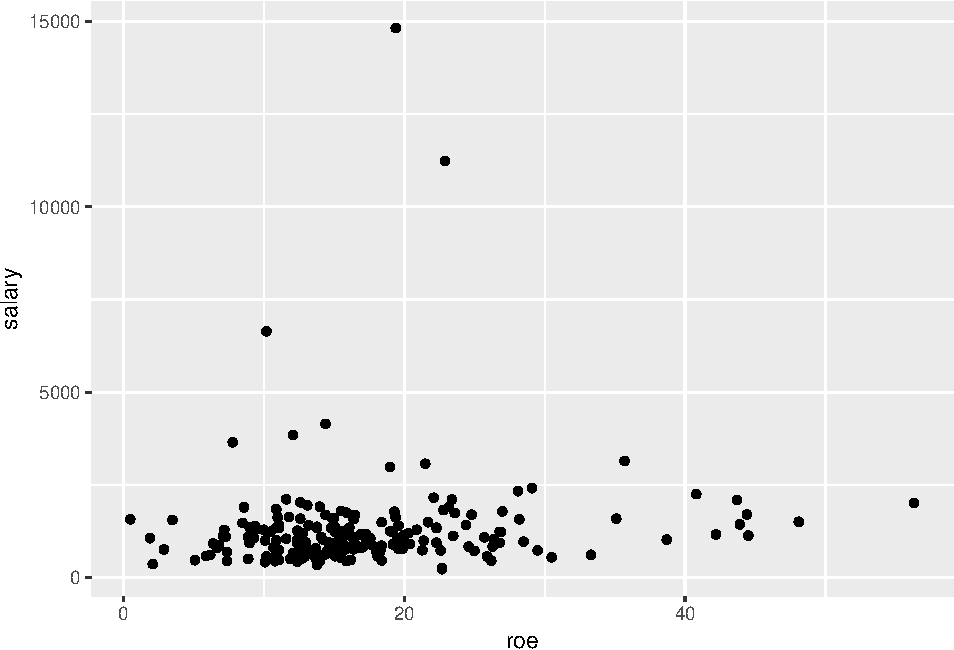
\includegraphics{MEM5220_R_files/figure-latex/ceosal1-1.pdf}
\caption{\label{fig:ceosal1}Relationship between ROE and Salary}
\end{figure}

Consider a simple regression model

\(salary = \beta_0 + \beta_1roe + u\)

In the general form the linear regression model can be written as:

\begin{equation}
y = \beta_{0} + \beta_{1}x + u
\label{eq:simplelinearregressionmodel}
\end{equation}

We are concerned with the population parameter \(\beta_{0}\) and
\(\beta_{1}\). The ordinary least squares (OLS) estimators are:

\begin{equation}
\hat{\beta}_{0} = \bar{y} - \hat{\beta}_{1}\bar{x}
\label{eq:populationparameterBeta0}
\end{equation}

The ordinary least squares (OLS) estimators are

\begin{equation}
\hat{\beta}_{1} = \frac{Cov(x,y)}{Var(x)}
\label{eq:populationparameterBeta1}
\end{equation}

Ingredients for the OLS formulas

\begin{Shaded}
\begin{Highlighting}[]
\KeywordTok{attach}\NormalTok{(ceosal1)}
\KeywordTok{cov}\NormalTok{(roe, salary)}
\end{Highlighting}
\end{Shaded}

\begin{verbatim}
## [1] 1342.538
\end{verbatim}

\begin{Shaded}
\begin{Highlighting}[]
\KeywordTok{var}\NormalTok{(roe)}
\end{Highlighting}
\end{Shaded}

\begin{verbatim}
## [1] 72.56499
\end{verbatim}

\begin{Shaded}
\begin{Highlighting}[]
\KeywordTok{mean}\NormalTok{(salary)}
\end{Highlighting}
\end{Shaded}

\begin{verbatim}
## [1] 1281.12
\end{verbatim}

Manual calculation of the OLS coefficients

\begin{Shaded}
\begin{Highlighting}[]
\NormalTok{b1hat <-}\StringTok{ }\KeywordTok{cov}\NormalTok{(roe,salary)}\OperatorTok{/}\KeywordTok{var}\NormalTok{(roe)}
\end{Highlighting}
\end{Shaded}

\begin{Shaded}
\begin{Highlighting}[]
\NormalTok{b0hat <-}\StringTok{ }\KeywordTok{mean}\NormalTok{(salary) }\OperatorTok{-}\StringTok{ }\NormalTok{b1hat }\OperatorTok{*}\StringTok{ }\KeywordTok{mean}\NormalTok{(roe)}
\end{Highlighting}
\end{Shaded}

Or use the \texttt{lm()} function

\begin{Shaded}
\begin{Highlighting}[]
\KeywordTok{lm}\NormalTok{(salary }\OperatorTok{~}\StringTok{ }\NormalTok{roe, }\DataTypeTok{data=}\NormalTok{ceosal1)}
\end{Highlighting}
\end{Shaded}

\begin{verbatim}
## 
## Call:
## lm(formula = salary ~ roe, data = ceosal1)
## 
## Coefficients:
## (Intercept)          roe  
##       963.2         18.5
\end{verbatim}

\begin{Shaded}
\begin{Highlighting}[]
\NormalTok{lm1_ceosal1 <-}\StringTok{ }\KeywordTok{lm}\NormalTok{(salary }\OperatorTok{~}\StringTok{ }\NormalTok{roe, }\DataTypeTok{data=}\NormalTok{ceosal1) }
\KeywordTok{summary}\NormalTok{(lm1_ceosal1)}
\end{Highlighting}
\end{Shaded}

\begin{verbatim}
## 
## Call:
## lm(formula = salary ~ roe, data = ceosal1)
## 
## Residuals:
##     Min      1Q  Median      3Q     Max 
## -1160.2  -526.0  -254.0   138.8 13499.9 
## 
## Coefficients:
##             Estimate Std. Error t value Pr(>|t|)    
## (Intercept)   963.19     213.24   4.517 1.05e-05 ***
## roe            18.50      11.12   1.663   0.0978 .  
## ---
## Signif. codes:  0 '***' 0.001 '**' 0.01 '*' 0.05 '.' 0.1 ' ' 1
## 
## Residual standard error: 1367 on 207 degrees of freedom
## Multiple R-squared:  0.01319,    Adjusted R-squared:  0.008421 
## F-statistic: 2.767 on 1 and 207 DF,  p-value: 0.09777
\end{verbatim}

Plot the linear regression fit the \emph{base} r way.

\begin{Shaded}
\begin{Highlighting}[]
\KeywordTok{plot}\NormalTok{(salary}\OperatorTok{~}\StringTok{ }\NormalTok{roe, }\DataTypeTok{data =}\NormalTok{ ceosal1,}
     \DataTypeTok{xlab =} \StringTok{"Return on equity"}\NormalTok{,}
     \DataTypeTok{ylab =} \StringTok{"Salary"}\NormalTok{,}
     \DataTypeTok{main =} \StringTok{"Salary vs return on equity"}\NormalTok{,}
     \DataTypeTok{pch  =} \DecValTok{20}\NormalTok{,}
     \DataTypeTok{cex  =} \DecValTok{2}\NormalTok{,}
     \DataTypeTok{col  =} \StringTok{"grey"}\NormalTok{)}
\KeywordTok{abline}\NormalTok{(lm1_ceosal1, }\DataTypeTok{lwd =} \DecValTok{3}\NormalTok{, }\DataTypeTok{col =} \StringTok{"darkorange"}\NormalTok{)}
\end{Highlighting}
\end{Shaded}

\begin{figure}

{\centering 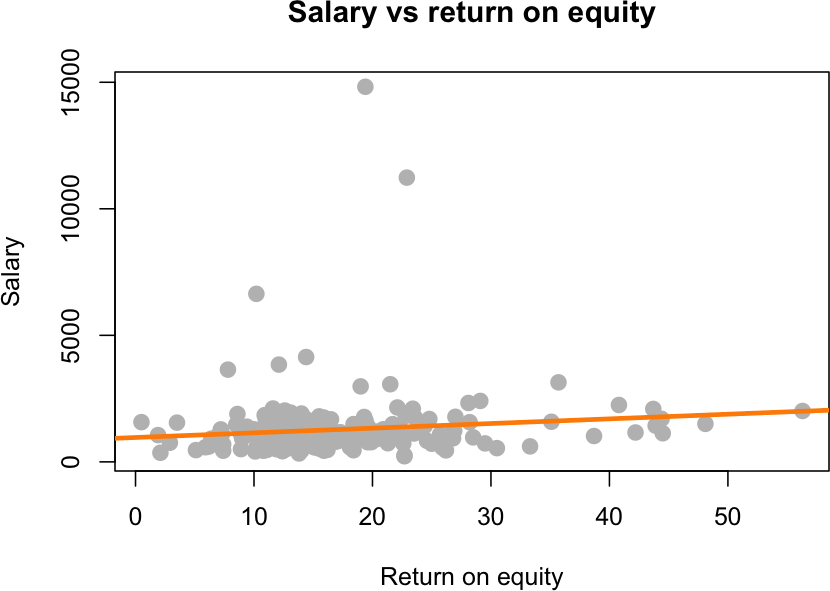
\includegraphics[width=0.8\linewidth]{MEM5220_R_files/figure-latex/fig1-1} 

}

\caption{OLS regression base Rstyle}\label{fig:fig1}
\end{figure}

Or use ggplot

\begin{Shaded}
\begin{Highlighting}[]
\KeywordTok{ggplot}\NormalTok{(ceosal1, }\KeywordTok{aes}\NormalTok{(}\DataTypeTok{x =}\NormalTok{ roe, }\DataTypeTok{y =}\NormalTok{ salary)) }\OperatorTok{+}\StringTok{ }
\StringTok{  }\KeywordTok{geom_point}\NormalTok{() }\OperatorTok{+}
\StringTok{  }\KeywordTok{stat_smooth}\NormalTok{(}\DataTypeTok{method =} \StringTok{"lm"}\NormalTok{, }\DataTypeTok{col =} \StringTok{"red"}\NormalTok{)}
\end{Highlighting}
\end{Shaded}

\begin{figure}

{\centering 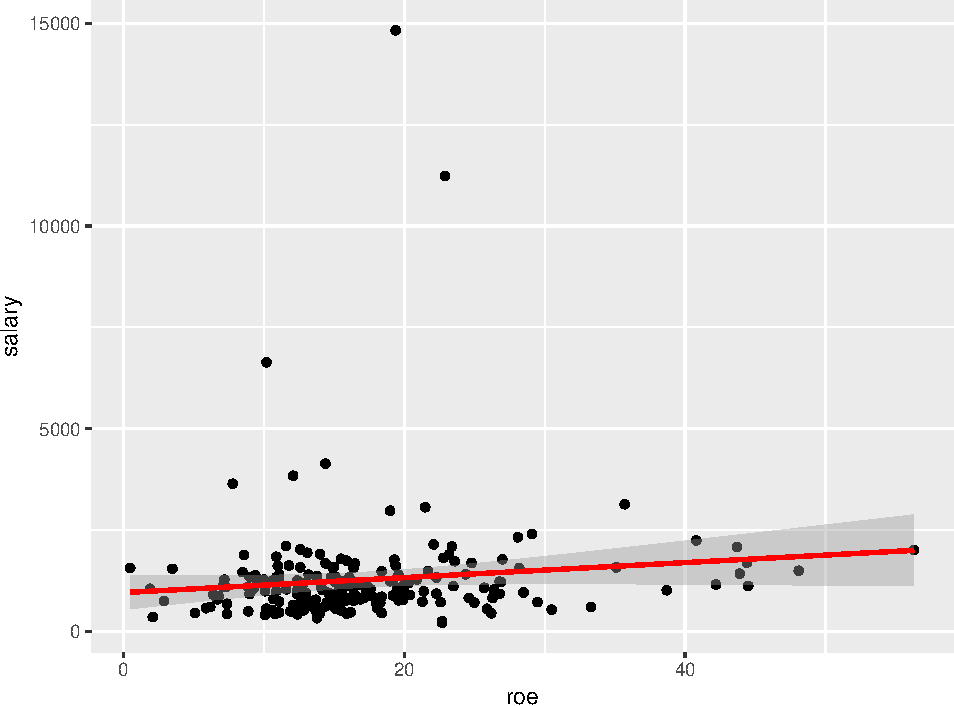
\includegraphics[width=0.8\linewidth]{MEM5220_R_files/figure-latex/fig2-1} 

}

\caption{OLS regression ggplot2 style}\label{fig:fig2}
\end{figure}

Determine the names of the elements of the list using the
\texttt{names()} command.

\begin{Shaded}
\begin{Highlighting}[]
\KeywordTok{names}\NormalTok{(lm1_ceosal1)}
\end{Highlighting}
\end{Shaded}

\begin{verbatim}
##  [1] "coefficients"  "residuals"     "effects"       "rank"         
##  [5] "fitted.values" "assign"        "qr"            "df.residual"  
##  [9] "xlevels"       "call"          "terms"         "model"
\end{verbatim}

Extract one element, for example the residuals from the list object

\begin{Shaded}
\begin{Highlighting}[]
\KeywordTok{head}\NormalTok{(lm1_ceosal1}\OperatorTok{$}\NormalTok{residuals) }\CommentTok{# head() just prints out the first 6 residual values}
\end{Highlighting}
\end{Shaded}

\begin{verbatim}
##         1         2         3         4         5         6 
## -129.0581 -163.8543 -275.9692 -494.3483  149.4923 -188.2151
\end{verbatim}

Another way to access stored information in \emph{lm1\_ceosal1} are the
\texttt{coef()}, \texttt{resid()}, and \texttt{fitted()} functions.
These return the coefficients, residuals, and fitted values,
respectively.

\begin{Shaded}
\begin{Highlighting}[]
\KeywordTok{coef}\NormalTok{(lm1_ceosal1)}
\end{Highlighting}
\end{Shaded}

\begin{verbatim}
## (Intercept)         roe 
##   963.19134    18.50119
\end{verbatim}

The function \texttt{summary()} is useful in many situations. We see
that when it is called on our model, it returns a good deal of
information.

\begin{Shaded}
\begin{Highlighting}[]
\KeywordTok{summary}\NormalTok{(lm1_ceosal1)}
\end{Highlighting}
\end{Shaded}

\begin{verbatim}
## 
## Call:
## lm(formula = salary ~ roe, data = ceosal1)
## 
## Residuals:
##     Min      1Q  Median      3Q     Max 
## -1160.2  -526.0  -254.0   138.8 13499.9 
## 
## Coefficients:
##             Estimate Std. Error t value Pr(>|t|)    
## (Intercept)   963.19     213.24   4.517 1.05e-05 ***
## roe            18.50      11.12   1.663   0.0978 .  
## ---
## Signif. codes:  0 '***' 0.001 '**' 0.01 '*' 0.05 '.' 0.1 ' ' 1
## 
## Residual standard error: 1367 on 207 degrees of freedom
## Multiple R-squared:  0.01319,    Adjusted R-squared:  0.008421 
## F-statistic: 2.767 on 1 and 207 DF,  p-value: 0.09777
\end{verbatim}

The \texttt{summary()} command also returns a list, and we can again use
\texttt{names()} to learn what about the elements of this list.

\begin{Shaded}
\begin{Highlighting}[]
\KeywordTok{names}\NormalTok{(}\KeywordTok{summary}\NormalTok{(lm1_ceosal1))}
\end{Highlighting}
\end{Shaded}

\begin{verbatim}
##  [1] "call"          "terms"         "residuals"     "coefficients" 
##  [5] "aliased"       "sigma"         "df"            "r.squared"    
##  [9] "adj.r.squared" "fstatistic"    "cov.unscaled"
\end{verbatim}

So, for example, if we wanted to directly access the value of \(R^2\),
instead of copy and pasting it out of the printed statement from
\texttt{summary()}, we could do so.

\begin{Shaded}
\begin{Highlighting}[]
\KeywordTok{summary}\NormalTok{(lm1_ceosal1)}\OperatorTok{$}\NormalTok{r.squared}
\end{Highlighting}
\end{Shaded}

\begin{verbatim}
## [1] 0.01318862
\end{verbatim}

\begin{center}\rule{0.5\linewidth}{\linethickness}\end{center}

\textbf{Your turn}

Recall that the explained sum of squares (SSE) is

\begin{equation}
SSE = \sum_{i=1}^{n}(\hat{y}_{i} - \bar{y})^2 = (n-1) \times Var(\hat{y})
\label{eq:SSE}
\end{equation}

and the residual sum of squares (SSR) is

\begin{equation}
R^2 = \frac{Var(\hat{y})}{Var(y)} = 1 - \frac{Var(\hat{u})}{Var(y)} 
\label{eq:SSR}
\end{equation}

One can see that the correlation between observed and fitted values is a
square root of \(R^2\).

Calculate \(R^2\) manually:

\begin{Shaded}
\begin{Highlighting}[]
\KeywordTok{var}\NormalTok{(}\KeywordTok{fitted}\NormalTok{(lm1_ceosal1))}\OperatorTok{/}\KeywordTok{var}\NormalTok{(ceosal1}\OperatorTok{$}\NormalTok{salary)}
\end{Highlighting}
\end{Shaded}

\begin{verbatim}
## [1] 0.01318862
\end{verbatim}

\begin{Shaded}
\begin{Highlighting}[]
\DecValTok{1} \OperatorTok{-}\StringTok{ }\KeywordTok{var}\NormalTok{(}\KeywordTok{residuals}\NormalTok{(lm1_ceosal1))}\OperatorTok{/}\KeywordTok{var}\NormalTok{(ceosal1}\OperatorTok{$}\NormalTok{salary)}
\end{Highlighting}
\end{Shaded}

\begin{verbatim}
## [1] 0.01318862
\end{verbatim}

\begin{center}\rule{0.5\linewidth}{\linethickness}\end{center}

Another useful function is the \texttt{predict()} function.

\begin{Shaded}
\begin{Highlighting}[]
\KeywordTok{set.seed}\NormalTok{(}\DecValTok{123}\NormalTok{)}
\CommentTok{# unique(ceosal1$roe)}
\NormalTok{roe_sample <-}\KeywordTok{sample}\NormalTok{(ceosal1}\OperatorTok{$}\NormalTok{roe, }\DecValTok{1}\NormalTok{)}
\NormalTok{roe_sample}
\end{Highlighting}
\end{Shaded}

\begin{verbatim}
## [1] 20.3
\end{verbatim}

Let's make a prediction for salary when the return on equity is
20.2999992.

\begin{Shaded}
\begin{Highlighting}[]
\NormalTok{b0hat_sample <-}\StringTok{ }\KeywordTok{mean}\NormalTok{(salary) }\OperatorTok{-}\StringTok{ }\NormalTok{b1hat }\OperatorTok{*}\StringTok{ }\NormalTok{roe_sample }
\end{Highlighting}
\end{Shaded}

We are not restricted to observed values of the explanatory variable.
Instead we can supply also our own predictor values

\begin{Shaded}
\begin{Highlighting}[]
\KeywordTok{predict}\NormalTok{(lm1_ceosal1, }\DataTypeTok{newdata =} \KeywordTok{data.frame}\NormalTok{(}\DataTypeTok{roe =} \DecValTok{30}\NormalTok{))}
\end{Highlighting}
\end{Shaded}

\begin{verbatim}
##        1 
## 1518.227
\end{verbatim}

The above code reads ``predict the salary when the return on equity is
30 using the \emph{lm1\_ceosal1} model.''

\begin{center}\rule{0.5\linewidth}{\linethickness}\end{center}

\textbf{Overthinking}

\hypertarget{regression-through-the-origin-and-regression-on-a-constant}{%
\subsection{Regression through the Origin and Regression on a
Constant}\label{regression-through-the-origin-and-regression-on-a-constant}}

Regression without intercept (through origin)

\begin{Shaded}
\begin{Highlighting}[]
\NormalTok{lm2 <-}\StringTok{ }\KeywordTok{lm}\NormalTok{(salary }\OperatorTok{~}\StringTok{  }\DecValTok{0} \OperatorTok{+}\StringTok{ }\NormalTok{roe, }\DataTypeTok{data =}\NormalTok{ ceosal1)}
\end{Highlighting}
\end{Shaded}

Regression without slope

\begin{Shaded}
\begin{Highlighting}[]
\NormalTok{lm3 <-}\StringTok{ }\KeywordTok{lm}\NormalTok{(salary }\OperatorTok{~}\StringTok{ }\DecValTok{1}\NormalTok{, }\DataTypeTok{data =}\NormalTok{ ceosal1)}
\end{Highlighting}
\end{Shaded}

\begin{Shaded}
\begin{Highlighting}[]
\KeywordTok{plot}\NormalTok{(salary}\OperatorTok{~}\StringTok{ }\NormalTok{roe, }\DataTypeTok{data =}\NormalTok{ ceosal1,}
     \DataTypeTok{xlab =} \StringTok{"Return on equity"}\NormalTok{,}
     \DataTypeTok{ylab =} \StringTok{"Salary"}\NormalTok{,}
     \DataTypeTok{main =} \StringTok{"Salary vs return on equity"}\NormalTok{,}
     \DataTypeTok{pch  =} \DecValTok{20}\NormalTok{,}
     \DataTypeTok{cex  =} \DecValTok{2}\NormalTok{,}
     \DataTypeTok{col  =} \StringTok{"grey"}\NormalTok{)}
\KeywordTok{abline}\NormalTok{(lm1_ceosal1, }\DataTypeTok{lwd =} \DecValTok{3}\NormalTok{, }\DataTypeTok{lty =} \DecValTok{1}\NormalTok{, }\DataTypeTok{col =} \StringTok{"darkorange"}\NormalTok{)}
\KeywordTok{abline}\NormalTok{(lm2,}\DataTypeTok{lwd =} \DecValTok{3}\NormalTok{,  }\DataTypeTok{lty =} \DecValTok{2}\NormalTok{,   }\DataTypeTok{col =} \StringTok{"darkblue"}\NormalTok{)}
\KeywordTok{abline}\NormalTok{(lm3, }\DataTypeTok{lwd =} \DecValTok{3}\NormalTok{,  }\DataTypeTok{lty =} \DecValTok{3}\NormalTok{,   }\DataTypeTok{col =} \StringTok{"black"}\NormalTok{)}
\KeywordTok{legend}\NormalTok{(}\StringTok{"topleft"}\NormalTok{, }
       \KeywordTok{c}\NormalTok{(}\StringTok{"full"}\NormalTok{, }
         \StringTok{"through origin"}\NormalTok{, }
         \StringTok{"constant only"}\NormalTok{), }
       \DataTypeTok{lwd =}\DecValTok{2}\NormalTok{, }
       \DataTypeTok{lty =} \DecValTok{1}\OperatorTok{:}\DecValTok{3}\NormalTok{)}
\end{Highlighting}
\end{Shaded}

\begin{figure}

{\centering 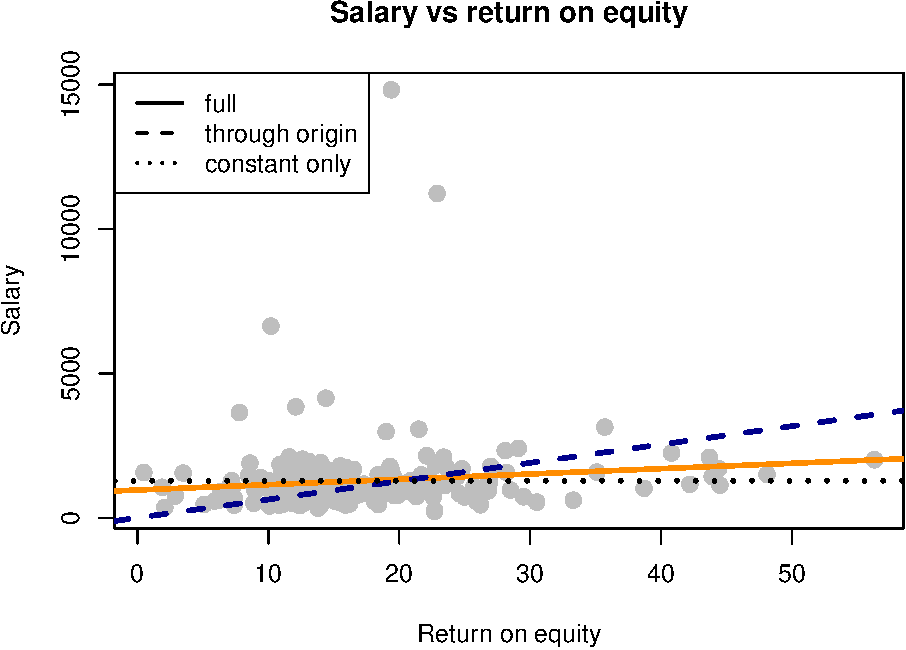
\includegraphics[width=0.8\linewidth]{MEM5220_R_files/figure-latex/fig3-1} 

}

\caption{Regression through the Origin and on a Constant}\label{fig:fig3}
\end{figure}

In models without the intercept the \(R^2\) loses its interpretatation.
The reason is that the \(R^2\) is the ratio of explained variance to
total variance \textbf{only} if the intercept is included.

\begin{center}\rule{0.5\linewidth}{\linethickness}\end{center}

\textbf{Overthinking}

\hypertarget{simulating-slr}{%
\subsection{Simulating SLR}\label{simulating-slr}}

\hypertarget{expected-values-variance-and-standard-errors}{%
\paragraph{Expected Values, Variance, and Standard
Errors}\label{expected-values-variance-and-standard-errors}}

The \textbf{Gauss--Markov theorem} tells us that when estimating the
parameters of the simple linear regression model \(\beta_{0}\) and
\(\beta_{1}\), the \(\hat{\beta}_{0}\) and \(\hat{\beta}_{1}\) which we
derived are the best linear unbiased estimates, or BLUE for short. (The
actual conditions for the Gauss--Markov theorem are more relaxed than
the SLR model.)

In short those assumptions are:

\begin{itemize}
\tightlist
\item
  SLR.1 Linear population regression function
  \(y = \beta_0 + \beta_{1} \times x + u\)
\item
  SLR.2 Random sampling of x and y from the population\\
\item
  SLR.3 Variation in the sample values: \(x_{1}, \dots , x_{n}\)
\item
  SLR.4 Zero conditional mean: \(\mathbf{E}(u|x) = 0\)
\item
  SLR.5 Homeskedasticity: \(Var(u|x) = \sigma^2\)
\end{itemize}

Recall that under \textbf{SLR.1 - SLR.4} the OLS parameter estimators
are unbiased. Under \textbf{SLR.1 - SLR.4} the OLS parameter estimators
have a specific sampling variance.

Simulating a model is an important concept. In practice you will almost
never have a true model, and you will use data to attempt to recover
information about the unknown true model. With simulation, we decide the
true model and simulate data from it. Then, we apply a method to the
data, in this case least squares. Now, since we know the true model, we
can assess how well it did.

Simulation also helps to grasp the concepts of estimators, estimates,
unbiasedness, the sampling variance of the estimators, and the
consequences of violated assumptions.

Sample size

\begin{Shaded}
\begin{Highlighting}[]
\NormalTok{n <-}\StringTok{ }\DecValTok{200}
\end{Highlighting}
\end{Shaded}

True parameters

\begin{Shaded}
\begin{Highlighting}[]
\NormalTok{b0<-}\StringTok{ }\DecValTok{1}
\NormalTok{b1 <-}\StringTok{ }\FloatTok{0.5}
\NormalTok{sigma <-}\StringTok{ }\DecValTok{2} \CommentTok{# standard deviation of the error term u }
\NormalTok{x1 <-}\StringTok{ }\DecValTok{5}
\end{Highlighting}
\end{Shaded}

Determine the distribution of the independent variable

\begin{Shaded}
\begin{Highlighting}[]
\NormalTok{yhat1 <-}\StringTok{ }\NormalTok{b0 }\OperatorTok{+}\StringTok{ }\NormalTok{b1 }\OperatorTok{*}\StringTok{ }\NormalTok{x1 }\CommentTok{#  Note that we do not include the error term }
\end{Highlighting}
\end{Shaded}

Plot a Gaussian distribution of the dependent variable based on the
parameters

\begin{Shaded}
\begin{Highlighting}[]
\KeywordTok{curve}\NormalTok{(}\KeywordTok{dnorm}\NormalTok{(x, }\DataTypeTok{mean =}\NormalTok{ yhat1, }\DataTypeTok{sd =}\NormalTok{ sigma), }\DecValTok{-5}\NormalTok{, }\DecValTok{15}\NormalTok{, }\DataTypeTok{col =} \StringTok{"blue"}\NormalTok{)}
\KeywordTok{abline}\NormalTok{(}\DataTypeTok{v =}\NormalTok{ yhat1, }\DataTypeTok{col =} \StringTok{"blue"}\NormalTok{, }\DataTypeTok{lty =} \DecValTok{2}\NormalTok{)}
\KeywordTok{legend}\NormalTok{(}\StringTok{"topright"}\NormalTok{, }\DataTypeTok{legend =} \KeywordTok{c}\NormalTok{(}\StringTok{"f(y|x = 5)"}\NormalTok{), }\DataTypeTok{lty =} \DecValTok{1}\NormalTok{, }\DataTypeTok{col =} \KeywordTok{c}\NormalTok{(}\StringTok{"blue"}\NormalTok{))}
\end{Highlighting}
\end{Shaded}

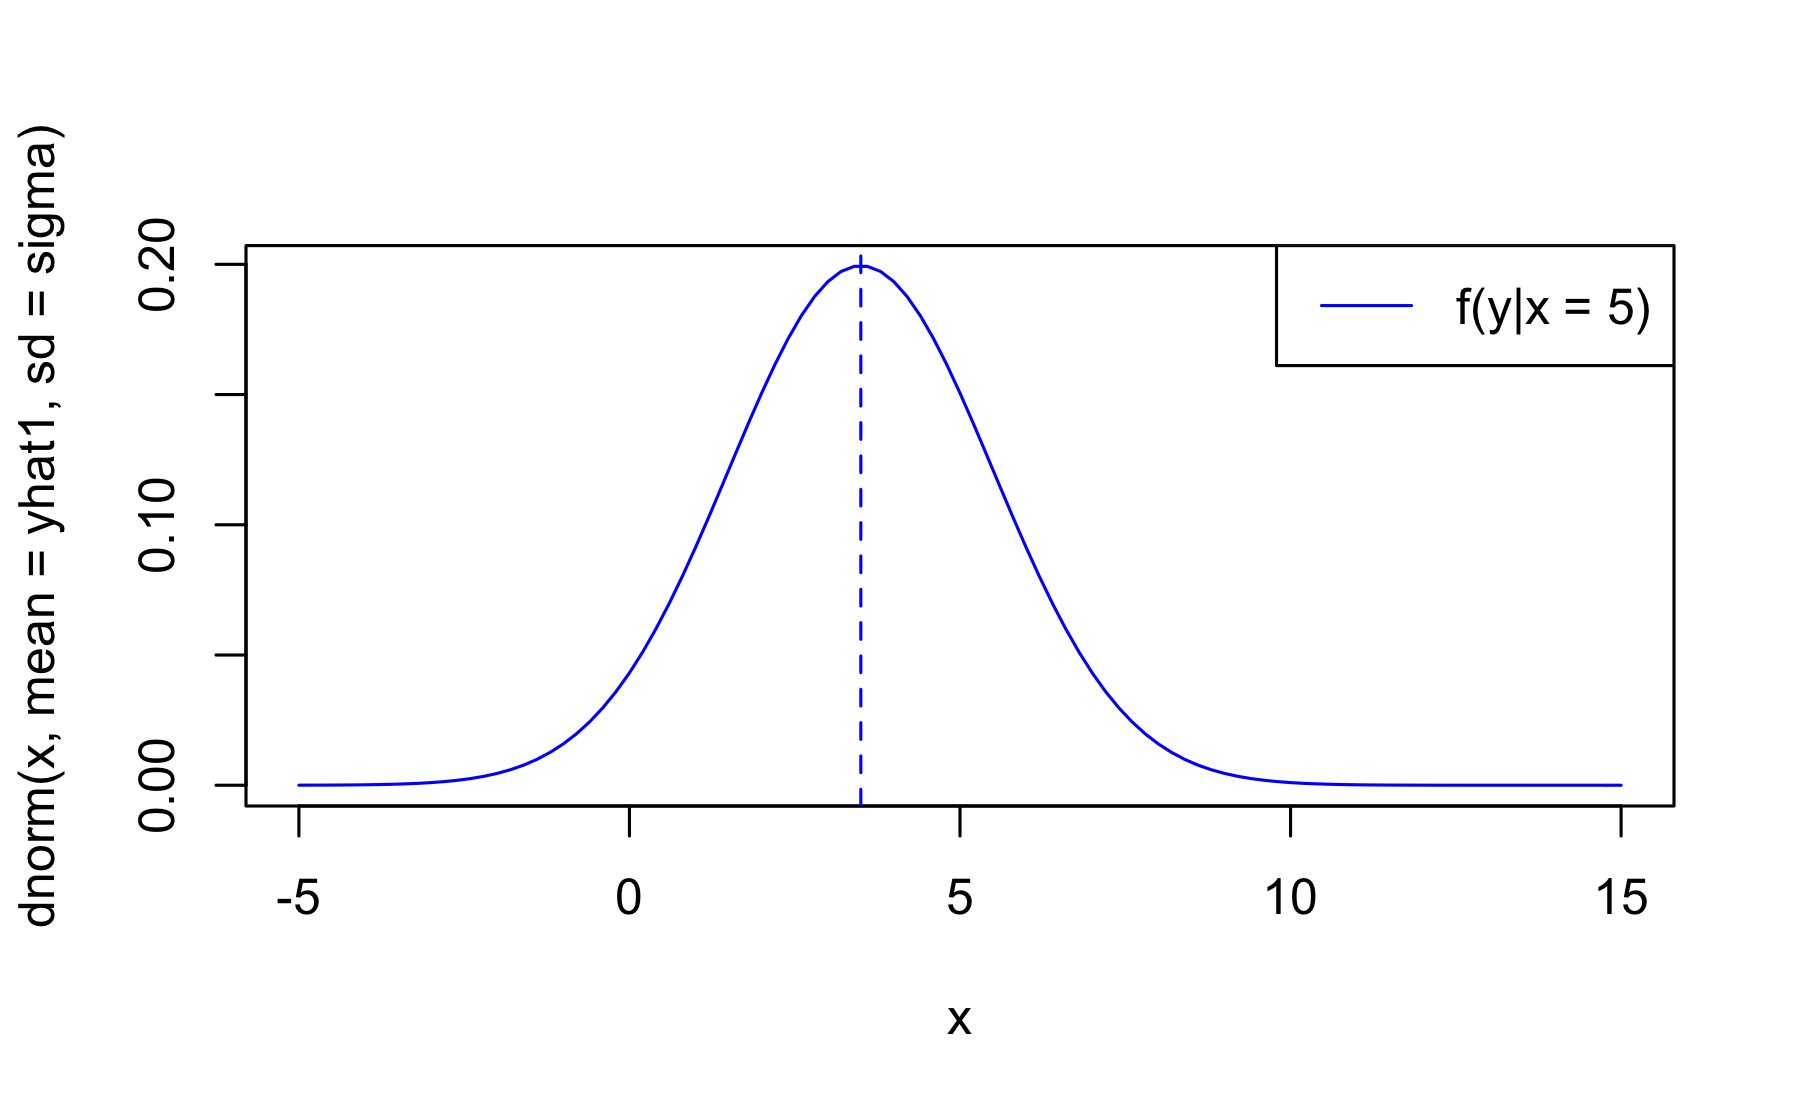
\includegraphics{MEM5220_R_files/figure-latex/unnamed-chunk-34-1.pdf}

This represent the theoretical (true) probability distribution of \(y\),
given \(x\)

We can calculate the variance of \(b_{1}\) and plot the corresponding
density function.

\begin{equation}
var(b_2) = \frac{\sigma^2}{\sum{}{}(x_1 - \bar{x})^2}
\label{eq:variancebeta}
\end{equation}

Assume that \(x_{2}\) represents a second possible predictor of \(y\)

\begin{Shaded}
\begin{Highlighting}[]
\NormalTok{x2 <-}\StringTok{ }\DecValTok{18}

\NormalTok{x <-}\StringTok{ }\KeywordTok{c}\NormalTok{(}\KeywordTok{rep}\NormalTok{(x1, n}\OperatorTok{/}\DecValTok{2}\NormalTok{), }\KeywordTok{rep}\NormalTok{(x2, n}\OperatorTok{/}\DecValTok{2}\NormalTok{))}
\NormalTok{xbar <-}\StringTok{ }\KeywordTok{mean}\NormalTok{(x)}

\NormalTok{sumxbar <-}\StringTok{ }\KeywordTok{sum}\NormalTok{((x}\OperatorTok{-}\NormalTok{xbar)}\OperatorTok{^}\DecValTok{2}\NormalTok{)}
\NormalTok{varb <-}\StringTok{ }\NormalTok{(sigma}\OperatorTok{^}\DecValTok{2}\NormalTok{)}\OperatorTok{/}\NormalTok{sumxbar}
\NormalTok{sdb <-}\KeywordTok{sqrt}\NormalTok{(varb)}
\NormalTok{leftlim <-}\StringTok{ }\NormalTok{b1}\DecValTok{-3}\OperatorTok{*}\NormalTok{sdb}
\NormalTok{rightlim <-}\StringTok{ }\NormalTok{b1}\OperatorTok{+}\DecValTok{3}\OperatorTok{*}\NormalTok{sdb}
\end{Highlighting}
\end{Shaded}

\begin{Shaded}
\begin{Highlighting}[]
\KeywordTok{curve}\NormalTok{(}\KeywordTok{dnorm}\NormalTok{(x, }\DataTypeTok{mean =}\NormalTok{ b1, }\DataTypeTok{sd =}\NormalTok{ sdb), leftlim, rightlim)}
\KeywordTok{abline}\NormalTok{(}\DataTypeTok{v =}\NormalTok{ b1, }\DataTypeTok{col =} \StringTok{"blue"}\NormalTok{, }\DataTypeTok{lty =} \DecValTok{2}\NormalTok{)}
\end{Highlighting}
\end{Shaded}

\begin{figure}

{\centering 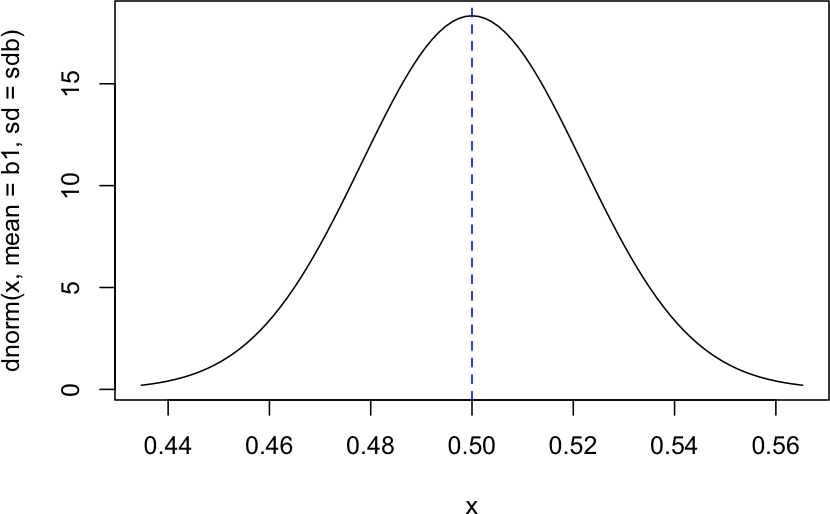
\includegraphics[width=0.8\linewidth]{MEM5220_R_files/figure-latex/fig4-1} 

}

\caption{The theoretical (true) probability density function of b1}\label{fig:fig4}
\end{figure}

Draw sample of size \(n\)

\begin{Shaded}
\begin{Highlighting}[]
\NormalTok{x <-}\StringTok{ }\KeywordTok{rnorm}\NormalTok{(n, }\DecValTok{4}\NormalTok{, sigma)}
\CommentTok{# Another way is to assume that the values for x are fixed and know}
\CommentTok{# x= seq(from = 0, to = 10, length.out = n)}
\end{Highlighting}
\end{Shaded}

\begin{Shaded}
\begin{Highlighting}[]
\NormalTok{u <-}\StringTok{ }\KeywordTok{rnorm}\NormalTok{(n, }\DecValTok{0}\NormalTok{, sigma)}
\end{Highlighting}
\end{Shaded}

\begin{Shaded}
\begin{Highlighting}[]
\NormalTok{y <-}\StringTok{ }\NormalTok{b0 }\OperatorTok{+}\StringTok{ }\NormalTok{b1 }\OperatorTok{*}\StringTok{ }\NormalTok{x }\OperatorTok{+}\StringTok{ }\NormalTok{u}
\end{Highlighting}
\end{Shaded}

Estimate parameter by OLS

\begin{Shaded}
\begin{Highlighting}[]
\NormalTok{olsreg <-}\StringTok{ }\KeywordTok{lm}\NormalTok{(y }\OperatorTok{~}\NormalTok{x )}
\end{Highlighting}
\end{Shaded}

\begin{Shaded}
\begin{Highlighting}[]
\NormalTok{simulation.df <-}\StringTok{ }\KeywordTok{data.frame}\NormalTok{(x,y)}
\NormalTok{population.df <-}\StringTok{ }\KeywordTok{data.frame}\NormalTok{(b0, b1)}
\end{Highlighting}
\end{Shaded}

\begin{Shaded}
\begin{Highlighting}[]
\KeywordTok{plot}\NormalTok{(simulation.df, }
     \DataTypeTok{xlab =} \StringTok{"x"}\NormalTok{,}
     \DataTypeTok{ylab =} \StringTok{"y"}\NormalTok{,}
     \CommentTok{# main = "Simulate least squares regression",}
     \DataTypeTok{pch  =} \DecValTok{20}\NormalTok{,}
     \DataTypeTok{cex  =} \DecValTok{2}\NormalTok{,}
     \DataTypeTok{col  =} \StringTok{"grey"}\NormalTok{)}
\KeywordTok{abline}\NormalTok{(olsreg, }\DataTypeTok{lwd =} \DecValTok{3}\NormalTok{, }\DataTypeTok{lty =} \DecValTok{1}\NormalTok{, }\DataTypeTok{col =} \StringTok{"darkorange"}\NormalTok{)}
\KeywordTok{abline}\NormalTok{(b0, b1,  }\DataTypeTok{lwd =} \DecValTok{3}\NormalTok{,  }\DataTypeTok{lty =} \DecValTok{2}\NormalTok{,   }\DataTypeTok{col =} \StringTok{"darkblue"}\NormalTok{)}
\KeywordTok{legend}\NormalTok{(}\StringTok{"topleft"}\NormalTok{, }
       \KeywordTok{c}\NormalTok{(}\StringTok{"OLS regression function"}\NormalTok{, }
         \StringTok{"Population regression function"}\NormalTok{), }
       \DataTypeTok{lwd =}\DecValTok{2}\NormalTok{, }
       \DataTypeTok{lty =} \DecValTok{1}\OperatorTok{:}\DecValTok{2}\NormalTok{)}
\end{Highlighting}
\end{Shaded}

\begin{figure}

{\centering 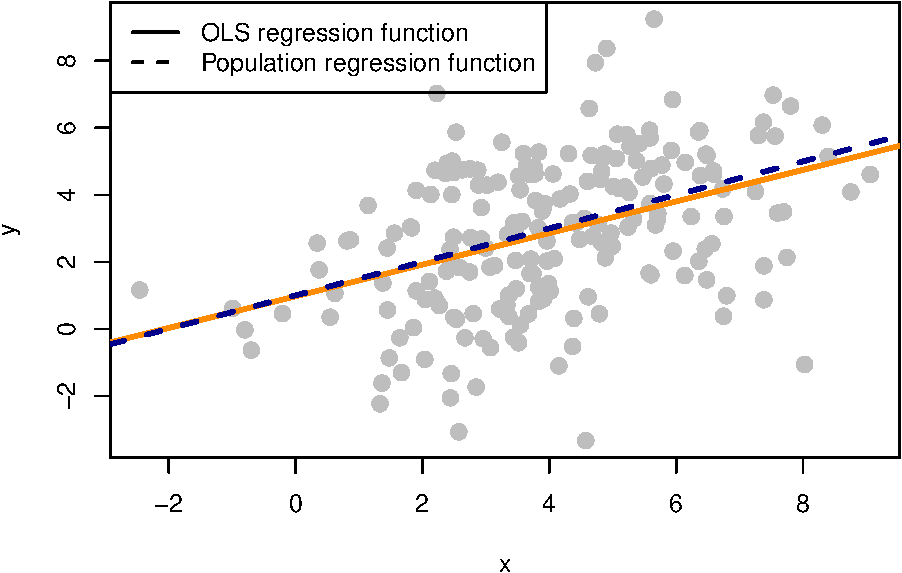
\includegraphics[width=0.8\linewidth]{MEM5220_R_files/figure-latex/fig5-1} 

}

\caption{Simulated Sample and OLS Regression Line}\label{fig:fig5}
\end{figure}

\begin{Shaded}
\begin{Highlighting}[]
\NormalTok{lable1 <-}\StringTok{ "OLS regression function"}
\KeywordTok{ggplot}\NormalTok{(simulation.df, }\KeywordTok{aes}\NormalTok{(}\DataTypeTok{x =}\NormalTok{ x,  }\DataTypeTok{y =}\NormalTok{ y)) }\OperatorTok{+}
\StringTok{  }\KeywordTok{geom_point}\NormalTok{() }\OperatorTok{+}
\StringTok{  }\KeywordTok{geom_abline}\NormalTok{(}\KeywordTok{aes}\NormalTok{(}\DataTypeTok{intercept=}\NormalTok{b0,}\DataTypeTok{slope=}\NormalTok{b1,}\DataTypeTok{colour=}\StringTok{"Population regression function"}\NormalTok{), }\DataTypeTok{linetype =}\StringTok{"dashed"}\NormalTok{, }\DataTypeTok{show.legend  =} \OtherTok{TRUE}\NormalTok{)}\OperatorTok{+}
\StringTok{  }\KeywordTok{stat_smooth}\NormalTok{(}\KeywordTok{aes}\NormalTok{(}\DataTypeTok{colour =}\StringTok{"OLS regression function"}\NormalTok{), }\DataTypeTok{method =} \StringTok{"lm"}\NormalTok{,}\DataTypeTok{se=}\OtherTok{FALSE}\NormalTok{, }\DataTypeTok{show.legend =}\OtherTok{TRUE}\NormalTok{)}\OperatorTok{+}
\StringTok{  }\KeywordTok{labs}\NormalTok{(}\DataTypeTok{colour =} \StringTok{"Regression functions"} 
       \CommentTok{# , title = "Simulate least squares regression"}
\NormalTok{  )}
\end{Highlighting}
\end{Shaded}

\begin{figure}

{\centering 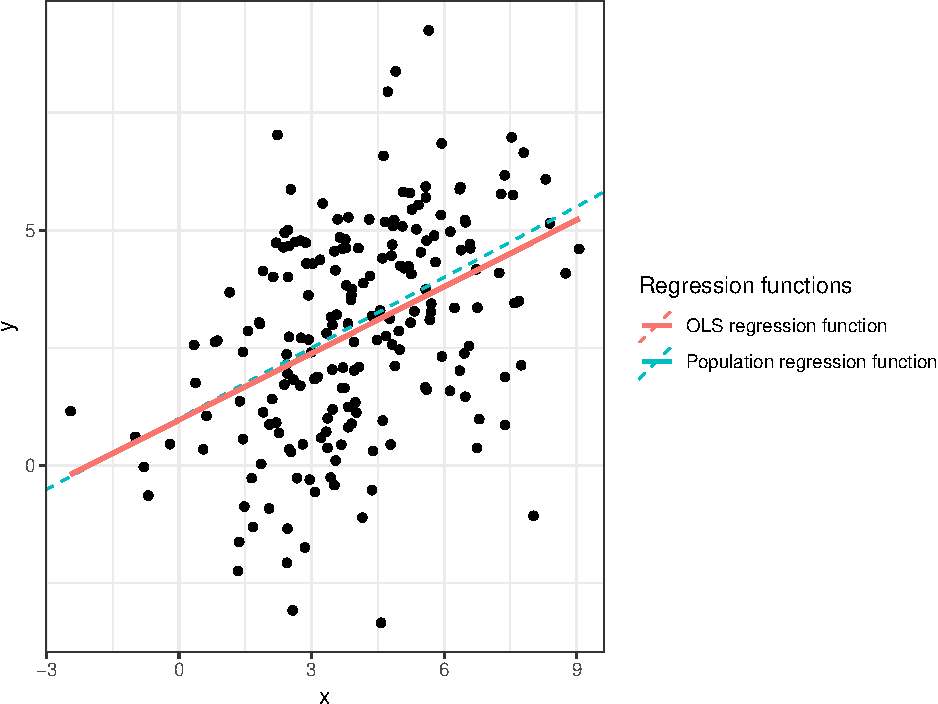
\includegraphics[width=0.8\linewidth]{MEM5220_R_files/figure-latex/fig6-1} 

}

\caption{Simulated Sample and OLS Regression Line (gpplot Style)}\label{fig:fig6}
\end{figure}

Since the expected values and variances of our estimators are defined
over separate random samples from the same population, it makes sense to
repeat our simulation exercise over many simulated samples.

\begin{Shaded}
\begin{Highlighting}[]
\CommentTok{# Set the random seed}
\KeywordTok{set.seed}\NormalTok{(}\DecValTok{1234567}\NormalTok{)}

\CommentTok{# set sample size and number of simulations}
\NormalTok{n<-}\DecValTok{1000}\NormalTok{; r<-}\DecValTok{10000}

\CommentTok{# set true parameters: betas and sd of u}
\NormalTok{b0<-}\FloatTok{1.0}\NormalTok{; b1<-}\FloatTok{0.5}\NormalTok{; sigma<-}\DecValTok{2}

\CommentTok{# initialize b0hat and b1hat to store results later:}
\NormalTok{b0hat <-}\StringTok{ }\KeywordTok{numeric}\NormalTok{(r)}
\NormalTok{b1hat <-}\StringTok{ }\KeywordTok{numeric}\NormalTok{(r)}

\CommentTok{# Draw a sample of x, fixed over replications:}
\NormalTok{x <-}\StringTok{ }\KeywordTok{rnorm}\NormalTok{(n,}\DecValTok{4}\NormalTok{,}\DecValTok{1}\NormalTok{)}

\CommentTok{# repeat r times:}
\ControlFlowTok{for}\NormalTok{(j }\ControlFlowTok{in} \DecValTok{1}\OperatorTok{:}\NormalTok{r) \{}
  \CommentTok{# Draw a sample of y:}
\NormalTok{  u <-}\StringTok{ }\KeywordTok{rnorm}\NormalTok{(n,}\DecValTok{0}\NormalTok{,sigma)}
\NormalTok{  y <-}\StringTok{ }\NormalTok{b0 }\OperatorTok{+}\StringTok{ }\NormalTok{b1}\OperatorTok{*}\NormalTok{x }\OperatorTok{+}\StringTok{ }\NormalTok{u}
  
  \CommentTok{# estimate parameters by OLS and store them in the vectors}
\NormalTok{  bhat <-}\StringTok{ }\KeywordTok{coefficients}\NormalTok{( }\KeywordTok{lm}\NormalTok{(y}\OperatorTok{~}\NormalTok{x) )}
\NormalTok{  b0hat[j] <-}\StringTok{ }\NormalTok{bhat[}\StringTok{"(Intercept)"}\NormalTok{]}
\NormalTok{  b1hat[j] <-}\StringTok{ }\NormalTok{bhat[}\StringTok{"x"}\NormalTok{]}
\NormalTok{\}}
\end{Highlighting}
\end{Shaded}

\begin{Shaded}
\begin{Highlighting}[]
\CommentTok{# MC estimate of the expected values:}
\KeywordTok{mean}\NormalTok{(b0hat)}
\end{Highlighting}
\end{Shaded}

\begin{verbatim}
## [1] 0.9985388
\end{verbatim}

\begin{Shaded}
\begin{Highlighting}[]
\KeywordTok{mean}\NormalTok{(b1hat)}
\end{Highlighting}
\end{Shaded}

\begin{verbatim}
## [1] 0.5000466
\end{verbatim}

\begin{Shaded}
\begin{Highlighting}[]
\CommentTok{# MC estimate of the variances:}
\KeywordTok{var}\NormalTok{(b0hat)}
\end{Highlighting}
\end{Shaded}

\begin{verbatim}
## [1] 0.0690833
\end{verbatim}

\begin{Shaded}
\begin{Highlighting}[]
\KeywordTok{var}\NormalTok{(b1hat)}
\end{Highlighting}
\end{Shaded}

\begin{verbatim}
## [1] 0.004069063
\end{verbatim}

\begin{Shaded}
\begin{Highlighting}[]
\CommentTok{# Initialize empty plot}
\KeywordTok{plot}\NormalTok{( }\OtherTok{NULL}\NormalTok{, }\DataTypeTok{xlim=}\KeywordTok{c}\NormalTok{(}\DecValTok{0}\NormalTok{,}\DecValTok{8}\NormalTok{), }\DataTypeTok{ylim=}\KeywordTok{c}\NormalTok{(}\DecValTok{0}\NormalTok{,}\DecValTok{6}\NormalTok{), }\DataTypeTok{xlab=}\StringTok{"x"}\NormalTok{, }\DataTypeTok{ylab=}\StringTok{"y"}\NormalTok{)}
\CommentTok{# add OLS regression lines}
\ControlFlowTok{for}\NormalTok{ (j }\ControlFlowTok{in} \DecValTok{1}\OperatorTok{:}\DecValTok{10}\NormalTok{) }\KeywordTok{abline}\NormalTok{(b0hat[j],b1hat[j],}\DataTypeTok{col=}\StringTok{"gray"}\NormalTok{)}
\CommentTok{# add population regression line}
\KeywordTok{abline}\NormalTok{(b0,b1,}\DataTypeTok{lwd=}\DecValTok{2}\NormalTok{)}
\CommentTok{# add legend}
\KeywordTok{legend}\NormalTok{(}\StringTok{"topleft"}\NormalTok{,}\KeywordTok{c}\NormalTok{(}\StringTok{"Population"}\NormalTok{,}\StringTok{"OLS regressions"}\NormalTok{),}
       \DataTypeTok{lwd=}\KeywordTok{c}\NormalTok{(}\DecValTok{2}\NormalTok{,}\DecValTok{1}\NormalTok{),}\DataTypeTok{col=}\KeywordTok{c}\NormalTok{(}\StringTok{"black"}\NormalTok{,}\StringTok{"gray"}\NormalTok{))}
\end{Highlighting}
\end{Shaded}

\begin{figure}

{\centering 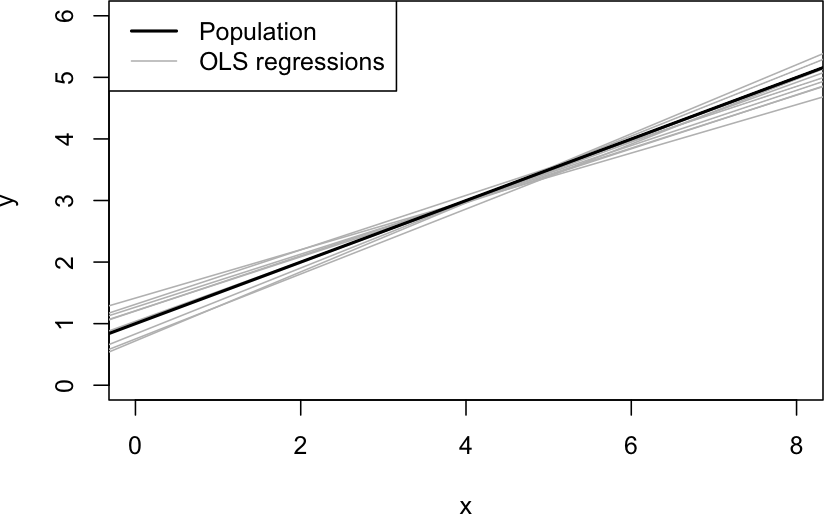
\includegraphics[width=0.8\linewidth]{MEM5220_R_files/figure-latex/fig7-1} 

}

\caption{Population and Simulated OLS Regression Lines}\label{fig:fig7}
\end{figure}

Even though the loop solution is transparent, let us take a look at a
different, more \emph{modern} approach.

\begin{Shaded}
\begin{Highlighting}[]
\CommentTok{# define a function the returns the alpha -- its point estimate, standard error, etc. -- from the OLS}
\NormalTok{x <-}\StringTok{ }\KeywordTok{rnorm}\NormalTok{(n,}\DecValTok{4}\NormalTok{,}\DecValTok{1}\NormalTok{) }\CommentTok{# }\AlertTok{NOTE}\CommentTok{ 1: Although a normal distribution is usually defined by its mean and variance, 'rnorm()' requires the standard deviation as input for the second moment.}
\CommentTok{# }\AlertTok{NOTE}\CommentTok{ 2: We use the same values for x in all samples since we draw them outside of the loop. }

\NormalTok{iteration <-}\StringTok{ }\ControlFlowTok{function}\NormalTok{() \{}
\NormalTok{  u <-}\StringTok{ }\KeywordTok{rnorm}\NormalTok{(n,}\DecValTok{0}\NormalTok{,sigma)}
\NormalTok{  y <-}\StringTok{ }\NormalTok{b0 }\OperatorTok{+}\StringTok{ }\NormalTok{b1}\OperatorTok{*}\NormalTok{x }\OperatorTok{+}\StringTok{ }\NormalTok{u}
  
  \KeywordTok{lm}\NormalTok{(y}\OperatorTok{~}\NormalTok{x) }\OperatorTok\StringTok{ }
\StringTok{    }\NormalTok{broom}\OperatorTok{::}\KeywordTok{tidy}\NormalTok{() }\CommentTok{# %>% }
  \CommentTok{# dplyr::filter(term == 'x') # One could only extract the slope}
\NormalTok{\}}

\CommentTok{# 1000 iterations of the above simulation}
\NormalTok{MC_coef<-}\StringTok{ }\KeywordTok{map_df}\NormalTok{(}\DecValTok{1}\OperatorTok{:}\DecValTok{1000}\NormalTok{, }\OperatorTok{~}\KeywordTok{iteration}\NormalTok{()) }
\KeywordTok{str}\NormalTok{(MC_coef)}
\end{Highlighting}
\end{Shaded}

\begin{verbatim}
## Classes 'tbl_df', 'tbl' and 'data.frame':    2000 obs. of  5 variables:
##  $ term     : chr  "(Intercept)" "x" "(Intercept)" "x" ...
##  $ estimate : num  1.577 0.372 1.44 0.387 1.355 ...
##  $ std.error: num  0.2672 0.0639 0.2623 0.0628 0.2626 ...
##  $ statistic: num  5.9 5.82 5.49 6.17 5.16 ...
##  $ p.value  : num  4.94e-09 7.91e-09 5.13e-08 9.92e-10 2.99e-07 ...
\end{verbatim}

Instead of plotting simulated and true parameter regression lines we can
take a look at the kernel density of the simulated parameter estimates

Figure \ref{fig:fig8} shows the simulated distribution of \(\beta_{0}\)
and \(\beta_{1}\) the theoretical one.

\begin{Shaded}
\begin{Highlighting}[]
\CommentTok{# plot the results}
\KeywordTok{str}\NormalTok{(MC_coef)}
\end{Highlighting}
\end{Shaded}

\begin{verbatim}
## Classes 'tbl_df', 'tbl' and 'data.frame':    2000 obs. of  5 variables:
##  $ term     : chr  "(Intercept)" "x" "(Intercept)" "x" ...
##  $ estimate : num  1.577 0.372 1.44 0.387 1.355 ...
##  $ std.error: num  0.2672 0.0639 0.2623 0.0628 0.2626 ...
##  $ statistic: num  5.9 5.82 5.49 6.17 5.16 ...
##  $ p.value  : num  4.94e-09 7.91e-09 5.13e-08 9.92e-10 2.99e-07 ...
\end{verbatim}

\begin{Shaded}
\begin{Highlighting}[]
\NormalTok{MC_coef<-}\StringTok{ }\NormalTok{MC_coef }\OperatorTok
\StringTok{  }\KeywordTok{mutate}\NormalTok{(}\DataTypeTok{OLScoeff =}  \KeywordTok{ifelse}\NormalTok{(term }\OperatorTok{==}\StringTok{ "x"}\NormalTok{, }\StringTok{"b1hat"}\NormalTok{, }\StringTok{"b0hat"}\NormalTok{)) }\OperatorTok\StringTok{  }\CommentTok{# rename the x to b1hat and (Intercept) to b0hat and create a new column }
\StringTok{  }\KeywordTok{mutate}\NormalTok{(}\DataTypeTok{Simulated =} \KeywordTok{ifelse}\NormalTok{(term }\OperatorTok{==}\StringTok{ "x"}\NormalTok{, }\StringTok{"b1"}\NormalTok{, }\StringTok{"b0"}\NormalTok{)) }\CommentTok{#  %>% }
\end{Highlighting}
\end{Shaded}

\begin{Shaded}
\begin{Highlighting}[]
\KeywordTok{ggplot}\NormalTok{(}\DataTypeTok{data=}\NormalTok{ MC_coef, }\KeywordTok{aes}\NormalTok{(estimate)) }\OperatorTok{+}\StringTok{ }
\StringTok{  }\KeywordTok{geom_histogram}\NormalTok{() }\OperatorTok{+}\StringTok{ }
\StringTok{  }\KeywordTok{geom_vline}\NormalTok{(}\DataTypeTok{data =}\NormalTok{ dplyr}\OperatorTok{::}\KeywordTok{filter}\NormalTok{(MC_coef, OLScoeff }\OperatorTok{==}\StringTok{ "b0hat"}\NormalTok{), }\KeywordTok{aes}\NormalTok{(}\DataTypeTok{xintercept=}\NormalTok{b0), }\DataTypeTok{colour=}\StringTok{"pink"}\NormalTok{)  }\OperatorTok{+}\StringTok{  }
\StringTok{  }\KeywordTok{geom_vline}\NormalTok{(}\DataTypeTok{data =}\NormalTok{ dplyr}\OperatorTok{::}\KeywordTok{filter}\NormalTok{(MC_coef, OLScoeff }\OperatorTok{==}\StringTok{ "b1hat"}\NormalTok{), }\KeywordTok{aes}\NormalTok{(}\DataTypeTok{xintercept=}\NormalTok{b1), }\DataTypeTok{colour=}\StringTok{"darkgreen"}\NormalTok{)  }\OperatorTok{+}\StringTok{ }
\StringTok{  }\KeywordTok{geom_text}\NormalTok{(}\DataTypeTok{data=}\NormalTok{MC_coef[}\DecValTok{3}\NormalTok{,], }\DataTypeTok{mapping=}\KeywordTok{aes}\NormalTok{(}\DataTypeTok{x=}\NormalTok{estimate, }\DataTypeTok{y=}\DecValTok{8}\NormalTok{, }\DataTypeTok{label=}\KeywordTok{paste}\NormalTok{(}\StringTok{"True parameter: "}\NormalTok{, MC_coef[}\DecValTok{3}\NormalTok{,}\DecValTok{7}\NormalTok{])), }\DataTypeTok{colour =} \StringTok{"pink"}\NormalTok{) }\OperatorTok{+}
\StringTok{  }\KeywordTok{geom_text}\NormalTok{(}\DataTypeTok{data=}\NormalTok{MC_coef[}\DecValTok{4}\NormalTok{,], }\DataTypeTok{mapping=}\KeywordTok{aes}\NormalTok{(}\DataTypeTok{x=}\NormalTok{estimate, }\DataTypeTok{y=}\DecValTok{8}\NormalTok{, }\DataTypeTok{label=}\KeywordTok{paste}\NormalTok{(}\StringTok{"True parameter: "}\NormalTok{, MC_coef[}\DecValTok{4}\NormalTok{,}\DecValTok{7}\NormalTok{])), }\DataTypeTok{colour =} \StringTok{"darkgreen"}\NormalTok{) }\OperatorTok{+}
\StringTok{  }\KeywordTok{facet_wrap}\NormalTok{( }\OperatorTok{~}\StringTok{ }\NormalTok{OLScoeff, }\DataTypeTok{scales =} \StringTok{"free"}\NormalTok{)   }\OperatorTok{+}
\StringTok{  }\KeywordTok{labs}\NormalTok{(}
    \DataTypeTok{title =} \StringTok{"Histogram Monte Carlo Simulations and True population parameters"}\NormalTok{) }\OperatorTok{+}
\StringTok{  }\KeywordTok{theme_bw}\NormalTok{()}
\end{Highlighting}
\end{Shaded}

\begin{verbatim}
## `stat_bin()` using `bins = 30`. Pick better value with `binwidth`.
\end{verbatim}

\begin{figure}

{\centering 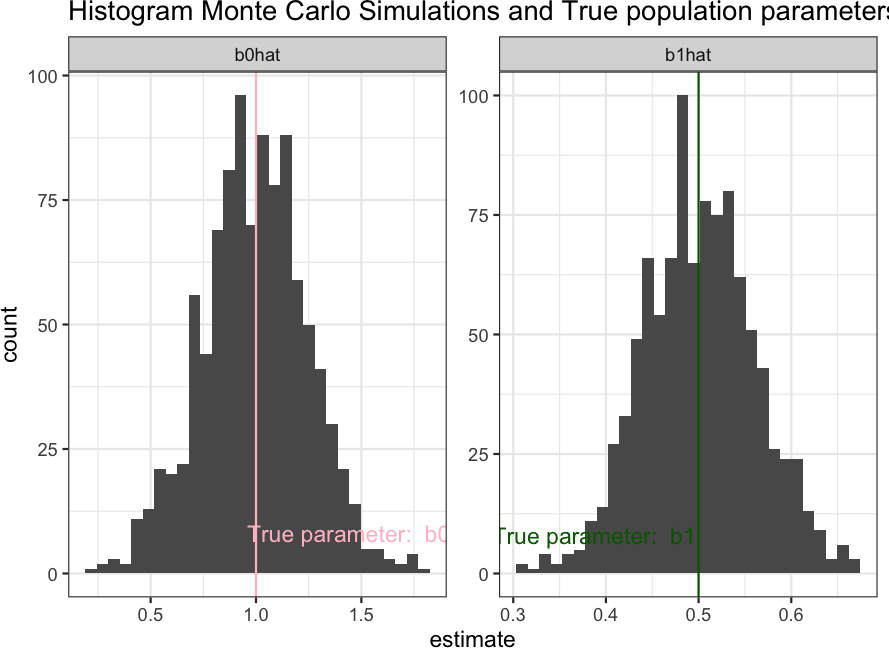
\includegraphics[width=0.8\linewidth]{MEM5220_R_files/figure-latex/fig8-1} 

}

\caption{Histogram b0 and b1 and true parameter}\label{fig:fig8}
\end{figure}

\begin{Shaded}
\begin{Highlighting}[]
\NormalTok{b1_sim <-}\StringTok{ }\NormalTok{MC_coef }\OperatorTok\StringTok{ }
\StringTok{  }\NormalTok{dplyr}\OperatorTok{::}\KeywordTok{filter}\NormalTok{(Simulated }\OperatorTok{==}\StringTok{ "b1"}\NormalTok{)}

\KeywordTok{mean}\NormalTok{(b1_sim}\OperatorTok{$}\NormalTok{estimate)}
\end{Highlighting}
\end{Shaded}

\begin{verbatim}
## [1] 0.5011414
\end{verbatim}

\begin{Shaded}
\begin{Highlighting}[]
\KeywordTok{var}\NormalTok{(b1_sim}\OperatorTok{$}\NormalTok{estimate) }\OperatorTok{==}\StringTok{ }\NormalTok{(}\KeywordTok{sd}\NormalTok{(b1_sim}\OperatorTok{$}\NormalTok{estimate))}\OperatorTok{^}\DecValTok{2}
\end{Highlighting}
\end{Shaded}

\begin{verbatim}
## [1] FALSE
\end{verbatim}

\begin{Shaded}
\begin{Highlighting}[]
\KeywordTok{all.equal}\NormalTok{(}\KeywordTok{var}\NormalTok{(b1_sim}\OperatorTok{$}\NormalTok{estimate) , (}\KeywordTok{sd}\NormalTok{(b1_sim}\OperatorTok{$}\NormalTok{estimate))}\OperatorTok{^}\DecValTok{2}\NormalTok{) }\CommentTok{# Floating point arithmetic!}
\end{Highlighting}
\end{Shaded}

\begin{verbatim}
## [1] TRUE
\end{verbatim}

\begin{Shaded}
\begin{Highlighting}[]
\KeywordTok{ggplot}\NormalTok{(}\DataTypeTok{data=}\NormalTok{ b1_sim, }\KeywordTok{aes}\NormalTok{(estimate)) }\OperatorTok{+}\StringTok{  }
\StringTok{  }\KeywordTok{geom_density}\NormalTok{(}\KeywordTok{aes}\NormalTok{(}\DataTypeTok{fill =}\NormalTok{ Simulated), }\DataTypeTok{alpha =} \FloatTok{0.2}\NormalTok{) }\OperatorTok{+}\StringTok{ }\CommentTok{# computes and draws the kernel density, which is the smoothed version of the histogram}
\StringTok{  }\CommentTok{# stat_function(fun = dnorm, args = list(mean = mean(b1_sim$estimate), sd = sd(b1_sim$estimate)), aes(colour = "true")) +}
\StringTok{  }\KeywordTok{stat_function}\NormalTok{(}\DataTypeTok{fun =}\NormalTok{ dnorm, }\DataTypeTok{args =} \KeywordTok{list}\NormalTok{(}\DataTypeTok{mean =} \FloatTok{0.5}\NormalTok{, }\DataTypeTok{sd =} \KeywordTok{sd}\NormalTok{(b1_sim}\OperatorTok{$}\NormalTok{estimate)), }\KeywordTok{aes}\NormalTok{(}\DataTypeTok{colour =} \StringTok{"Population"}\NormalTok{)) }\OperatorTok{+}
\StringTok{  }\CommentTok{# labs(}
\StringTok{  }\CommentTok{#  title = "Kernel Density Monte Carlo Simulations vs. True population parameters"}
\StringTok{  }\CommentTok{# ) +}
\StringTok{  }\KeywordTok{scale_color_discrete}\NormalTok{(}\DataTypeTok{name=}\StringTok{""}\NormalTok{)}
\end{Highlighting}
\end{Shaded}

\begin{figure}

{\centering 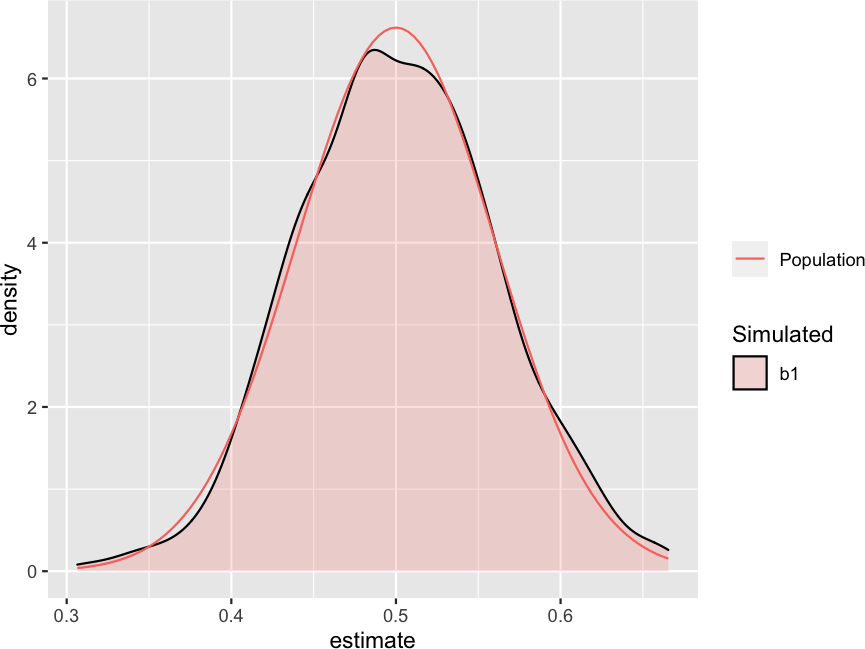
\includegraphics[width=0.8\linewidth]{MEM5220_R_files/figure-latex/fig9-1} 

}

\caption{Kernel Density Monte Carlo Simulations vs. True population parameters of b1}\label{fig:fig9}
\end{figure}

\hypertarget{violation-of-slr.4}{%
\paragraph{Violation of SLR.4}\label{violation-of-slr.4}}

To implement a violation of \textbf{SLR.4} (zero conditional mean)
consider a case where in the population \(u\) is not mean independent of
\(x\), for example

\[
\mathbf{E}(u|x) = \frac{x-4}{5}
\]

\begin{Shaded}
\begin{Highlighting}[]
\CommentTok{# Set the random seed}
\KeywordTok{set.seed}\NormalTok{(}\DecValTok{1234567}\NormalTok{)}

\CommentTok{# set sample size and number of simulations}
\NormalTok{n<-}\DecValTok{1000}\NormalTok{; r<-}\DecValTok{10000}

\CommentTok{# set true parameters: betas and sd of u}
\NormalTok{b0<-}\DecValTok{1}\NormalTok{; b1<-}\FloatTok{0.5}\NormalTok{; su<-}\DecValTok{2}

\CommentTok{# initialize b0hat and b1hat to store results later:}
\NormalTok{b0hat <-}\StringTok{ }\KeywordTok{numeric}\NormalTok{(r)}
\NormalTok{b1hat <-}\StringTok{ }\KeywordTok{numeric}\NormalTok{(r)}

\CommentTok{# Draw a sample of x, fixed over replications:}
\NormalTok{x <-}\StringTok{ }\KeywordTok{rnorm}\NormalTok{(n,}\DecValTok{4}\NormalTok{,}\DecValTok{1}\NormalTok{)}

\CommentTok{# repeat r times:}
\ControlFlowTok{for}\NormalTok{(j }\ControlFlowTok{in} \DecValTok{1}\OperatorTok{:}\NormalTok{r) \{}
  \CommentTok{# Draw a sample of y:}
\NormalTok{  u <-}\StringTok{ }\KeywordTok{rnorm}\NormalTok{(n, (x}\DecValTok{-4}\NormalTok{)}\OperatorTok{/}\DecValTok{5}\NormalTok{, su) }\CommentTok{# this is where manipulate the assumption of zero conditional mean}
\NormalTok{  y <-}\StringTok{ }\NormalTok{b0 }\OperatorTok{+}\StringTok{ }\NormalTok{b1}\OperatorTok{*}\NormalTok{x }\OperatorTok{+}\StringTok{ }\NormalTok{u}
  
  \CommentTok{# estimate parameters by OLS and store them in the vectors}
\NormalTok{  bhat <-}\StringTok{ }\KeywordTok{coefficients}\NormalTok{( }\KeywordTok{lm}\NormalTok{(y}\OperatorTok{~}\NormalTok{x) )}
\NormalTok{  b0hat[j] <-}\StringTok{ }\NormalTok{bhat[}\StringTok{"(Intercept)"}\NormalTok{]}
\NormalTok{  b1hat[j] <-}\StringTok{ }\NormalTok{bhat[}\StringTok{"x"}\NormalTok{]}
\NormalTok{\}}
\end{Highlighting}
\end{Shaded}

OLS coefficients

\begin{Shaded}
\begin{Highlighting}[]
\CommentTok{# MC estimate of the expected values:}
\KeywordTok{mean}\NormalTok{(b0hat)}
\end{Highlighting}
\end{Shaded}

\begin{verbatim}
## [1] 0.1985388
\end{verbatim}

\begin{Shaded}
\begin{Highlighting}[]
\KeywordTok{mean}\NormalTok{(b1hat)}
\end{Highlighting}
\end{Shaded}

\begin{verbatim}
## [1] 0.7000466
\end{verbatim}

\begin{Shaded}
\begin{Highlighting}[]
\CommentTok{# MC estimate of the variances:}
\KeywordTok{var}\NormalTok{(b0hat)}
\end{Highlighting}
\end{Shaded}

\begin{verbatim}
## [1] 0.0690833
\end{verbatim}

\begin{Shaded}
\begin{Highlighting}[]
\KeywordTok{var}\NormalTok{(b1hat)}
\end{Highlighting}
\end{Shaded}

\begin{verbatim}
## [1] 0.004069063
\end{verbatim}

The average estimates are far from the population parameters
\(\beta_0=1\) and \(\beta_1 = 0.5\)!

\hypertarget{violation-of-slr.5}{%
\paragraph{Violation of SLR.5}\label{violation-of-slr.5}}

Homoskedasticity is not required for unbiasedness but for it is a
requirement for the theorem of sampling variance. Consider the following
heteroskedastic behavior of \(u\) given \(x\).

\begin{Shaded}
\begin{Highlighting}[]
\CommentTok{# Set the random seed}
\KeywordTok{set.seed}\NormalTok{(}\DecValTok{1234567}\NormalTok{)}

\CommentTok{# set sample size and number of simulations}
\NormalTok{n<-}\DecValTok{1000}\NormalTok{; r<-}\DecValTok{10000}

\CommentTok{# set true parameters: betas and sd of u}
\NormalTok{b0<-}\DecValTok{1}\NormalTok{; b1<-}\FloatTok{0.5}\NormalTok{; su<-}\DecValTok{2}

\CommentTok{# initialize b0hat and b1hat to store results later:}
\NormalTok{b0hat <-}\StringTok{ }\KeywordTok{numeric}\NormalTok{(r)}
\NormalTok{b1hat <-}\StringTok{ }\KeywordTok{numeric}\NormalTok{(r)}

\CommentTok{# Draw a sample of x, fixed over replications:}
\NormalTok{x <-}\StringTok{ }\KeywordTok{rnorm}\NormalTok{(n,}\DecValTok{4}\NormalTok{,}\DecValTok{1}\NormalTok{)}

\CommentTok{# repeat r times:}
\ControlFlowTok{for}\NormalTok{(j }\ControlFlowTok{in} \DecValTok{1}\OperatorTok{:}\NormalTok{r) \{}
  \CommentTok{# Draw a sample of y:}
\NormalTok{  varu <-}\StringTok{ }\DecValTok{4}\OperatorTok{/}\KeywordTok{exp}\NormalTok{(}\FloatTok{4.5}\NormalTok{) }\OperatorTok{*}\StringTok{ }\KeywordTok{exp}\NormalTok{(x)}
\NormalTok{  u <-}\StringTok{ }\KeywordTok{rnorm}\NormalTok{(n, }\DecValTok{0}\NormalTok{, }\KeywordTok{sqrt}\NormalTok{(varu) )}
\NormalTok{  y <-}\StringTok{ }\NormalTok{b0 }\OperatorTok{+}\StringTok{ }\NormalTok{b1}\OperatorTok{*}\NormalTok{x }\OperatorTok{+}\StringTok{ }\NormalTok{u}
  
  \CommentTok{# estimate parameters by OLS and store them in the vectors}
\NormalTok{  lm_heterosced <-}\StringTok{ }\KeywordTok{lm}\NormalTok{(y}\OperatorTok{~}\NormalTok{x)}
  
\NormalTok{  bhat <-}\StringTok{ }\KeywordTok{coefficients}\NormalTok{( }\KeywordTok{lm}\NormalTok{(y}\OperatorTok{~}\NormalTok{x) )}
\NormalTok{  b0hat[j] <-}\StringTok{ }\NormalTok{bhat[}\StringTok{"(Intercept)"}\NormalTok{]}
\NormalTok{  b1hat[j] <-}\StringTok{ }\NormalTok{bhat[}\StringTok{"x"}\NormalTok{]}
\NormalTok{\}}
\end{Highlighting}
\end{Shaded}

\begin{Shaded}
\begin{Highlighting}[]
\KeywordTok{summary}\NormalTok{(lm_heterosced) }\CommentTok{# just the last sample of the MC-simulation}
\end{Highlighting}
\end{Shaded}

\begin{verbatim}
## 
## Call:
## lm(formula = y ~ x)
## 
## Residuals:
##      Min       1Q   Median       3Q      Max 
## -23.6742  -0.9033   0.0052   1.0012   9.3411 
## 
## Coefficients:
##             Estimate Std. Error t value Pr(>|t|)    
## (Intercept)  1.24088    0.27158   4.569 5.51e-06 ***
## x            0.44561    0.06593   6.759 2.37e-11 ***
## ---
## Signif. codes:  0 '***' 0.001 '**' 0.01 '*' 0.05 '.' 0.1 ' ' 1
## 
## Residual standard error: 2.075 on 998 degrees of freedom
## Multiple R-squared:  0.04377,    Adjusted R-squared:  0.04281 
## F-statistic: 45.68 on 1 and 998 DF,  p-value: 2.367e-11
\end{verbatim}

Plot the residual against the regressor suspected of creating
heteroskedasticity, or more generally, the fitted values of the
regression.

\begin{Shaded}
\begin{Highlighting}[]
\NormalTok{res <-}\StringTok{ }\KeywordTok{residuals}\NormalTok{(lm_heterosced)}
\NormalTok{yhat <-}\StringTok{ }\KeywordTok{fitted}\NormalTok{(lm_heterosced)}
\end{Highlighting}
\end{Shaded}

\begin{Shaded}
\begin{Highlighting}[]
\KeywordTok{par}\NormalTok{(}\DataTypeTok{mfrow =} \KeywordTok{c}\NormalTok{(}\DecValTok{1}\NormalTok{,}\DecValTok{2}\NormalTok{))}
\KeywordTok{plot}\NormalTok{(x, res, }\DataTypeTok{ylab =} \StringTok{"residuals"}\NormalTok{)}
\KeywordTok{plot}\NormalTok{(yhat, res, }\DataTypeTok{xlab =} \StringTok{"fitted values"}\NormalTok{, }\DataTypeTok{ylab =} \StringTok{"residuals"}\NormalTok{)}
\end{Highlighting}
\end{Shaded}

\begin{figure}

{\centering 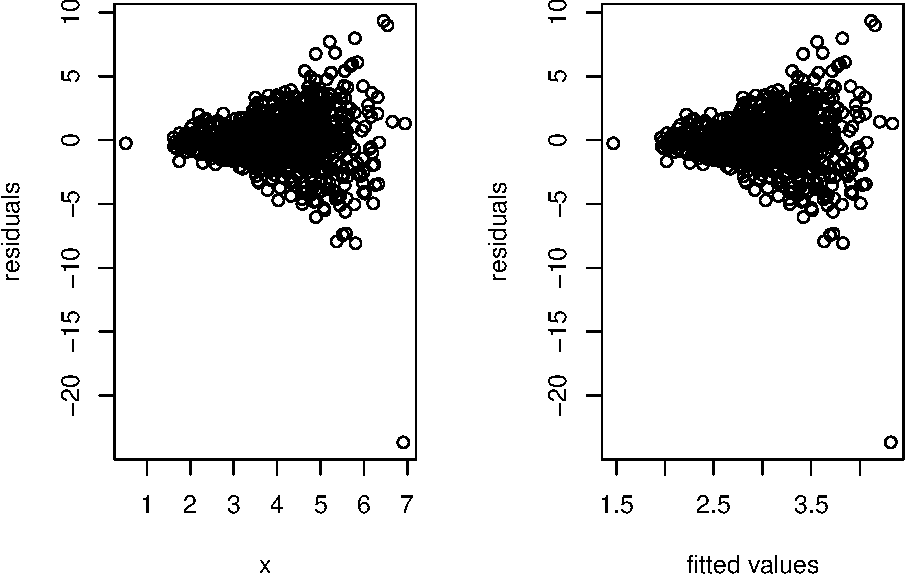
\includegraphics[width=0.8\linewidth]{MEM5220_R_files/figure-latex/fig10-1} 

}

\caption{Heteroskedasticity in the simulated data}\label{fig:fig10}
\end{figure}

\begin{Shaded}
\begin{Highlighting}[]
\CommentTok{# MC estimate of the expected values:}
\KeywordTok{mean}\NormalTok{(b0hat)}
\end{Highlighting}
\end{Shaded}

\begin{verbatim}
## [1] 1.0019
\end{verbatim}

\begin{Shaded}
\begin{Highlighting}[]
\KeywordTok{mean}\NormalTok{(b1hat)}
\end{Highlighting}
\end{Shaded}

\begin{verbatim}
## [1] 0.4992376
\end{verbatim}

\begin{Shaded}
\begin{Highlighting}[]
\CommentTok{# MC estimate of the variances:}
\KeywordTok{var}\NormalTok{(b0hat)}
\end{Highlighting}
\end{Shaded}

\begin{verbatim}
## [1] 0.08967037
\end{verbatim}

\begin{Shaded}
\begin{Highlighting}[]
\KeywordTok{var}\NormalTok{(b1hat)}
\end{Highlighting}
\end{Shaded}

\begin{verbatim}
## [1] 0.007264373
\end{verbatim}

Unbiasedness is provided but sampling variance is incorrect (compared to
the results provided above).

\begin{center}\rule{0.5\linewidth}{\linethickness}\end{center}

\hypertarget{nonlinearities}{%
\subsection{Nonlinearities}\label{nonlinearities}}

Sometimes the scatter plot diagram or some theoretical considerations
suggest a non-linear relationship. The most popular non-linear
transformation involve logarithms of the dependent or independent
variables and polynomial functions.

We will use a new dataset, \emph{wage1}, for this section. A detailed
exploratory analysis of the dataset is left to the reader.

\begin{Shaded}
\begin{Highlighting}[]
\KeywordTok{data}\NormalTok{(}\StringTok{"wage1"}\NormalTok{)}
\end{Highlighting}
\end{Shaded}

\hypertarget{predictor-variable-transformation}{%
\subsubsection{Predictor variable
transformation}\label{predictor-variable-transformation}}

A common variance stabilizing transformation (VST) is necessary when we
see increasing variance in a fitted versus residuals plot.

To use the \emph{log} of an independent variable is to make its
distribution closer to the normal distribution.

\begin{Shaded}
\begin{Highlighting}[]
\CommentTok{# wage1$logwage <- log(wage1$wage) # one could also create a new variable }

\NormalTok{p1_wagehisto <-}\StringTok{ }\KeywordTok{ggplot}\NormalTok{(wage1)  }\OperatorTok{+}
\StringTok{  }\KeywordTok{geom_histogram}\NormalTok{(}\KeywordTok{aes}\NormalTok{(}\DataTypeTok{x =}\NormalTok{ wage), }\DataTypeTok{fill =} \StringTok{"red"}\NormalTok{, }\DataTypeTok{alpha =} \FloatTok{0.6}\NormalTok{)}

\NormalTok{p2_wagehisto <-}\StringTok{ }\KeywordTok{ggplot}\NormalTok{(wage1)  }\OperatorTok{+}
\StringTok{  }\KeywordTok{geom_histogram}\NormalTok{(}\KeywordTok{aes}\NormalTok{(}\DataTypeTok{x =}\NormalTok{ wage),  }\DataTypeTok{fill =} \StringTok{"blue"}\NormalTok{, }\DataTypeTok{alpha =} \FloatTok{0.6}\NormalTok{) }\OperatorTok{+}
\StringTok{  }\KeywordTok{scale_x_continuous}\NormalTok{(}\DataTypeTok{trans=}\StringTok{'log2'}\NormalTok{, }\StringTok{"Log Wage"}\NormalTok{)  }\CommentTok{# instead of creating a new variable with simply define that the x-scale undergoes a logarithmic transformation}
\end{Highlighting}
\end{Shaded}

\begin{Shaded}
\begin{Highlighting}[]
\KeywordTok{ggarrange}\NormalTok{(p1_wagehisto, p2_wagehisto,  }
          \DataTypeTok{labels =} \KeywordTok{c}\NormalTok{(}\StringTok{"A"}\NormalTok{, }\StringTok{"B"}\NormalTok{),}
          \DataTypeTok{ncol =} \DecValTok{2}\NormalTok{, }\DataTypeTok{nrow =} \DecValTok{1}\NormalTok{)}
\end{Highlighting}
\end{Shaded}

\begin{verbatim}
## `stat_bin()` using `bins = 30`. Pick better value with `binwidth`.
## `stat_bin()` using `bins = 30`. Pick better value with `binwidth`.
\end{verbatim}

\begin{figure}

{\centering 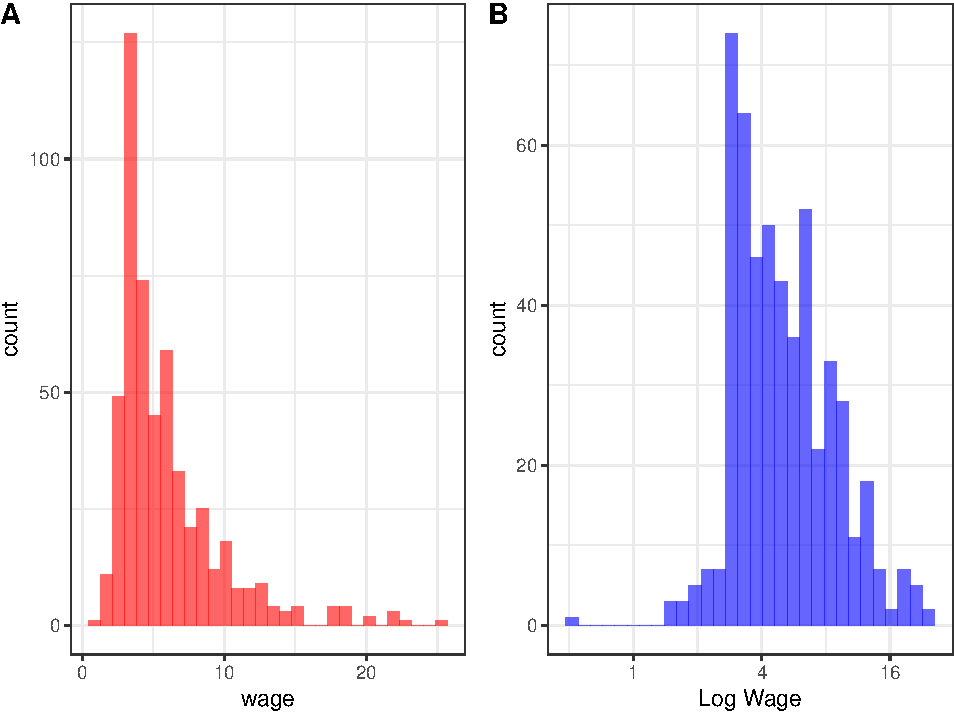
\includegraphics[width=0.8\linewidth]{MEM5220_R_files/figure-latex/fig11-1} 

}

\caption{Histogram of wage and log(wage)}\label{fig:fig11}
\end{figure}

A model with a log transformed response:

\begin{equation}
log(Y_{i}) = \beta_{0} + \beta_{1} \times x_{i} + \epsilon_{i}
\end{equation}

\begin{Shaded}
\begin{Highlighting}[]
\NormalTok{lm_wage <-}\StringTok{ }\KeywordTok{lm}\NormalTok{(wage }\OperatorTok{~}\StringTok{ }\NormalTok{educ, }\DataTypeTok{data =}\NormalTok{ wage1)}
\NormalTok{lm_wage1 <-}\StringTok{ }\KeywordTok{lm}\NormalTok{(}\KeywordTok{log}\NormalTok{(wage) }\OperatorTok{~}\StringTok{ }\NormalTok{educ, }\DataTypeTok{data =}\NormalTok{  wage1)}
\KeywordTok{summary}\NormalTok{(lm_wage)}
\end{Highlighting}
\end{Shaded}

\begin{verbatim}
## 
## Call:
## lm(formula = wage ~ educ, data = wage1)
## 
## Residuals:
##     Min      1Q  Median      3Q     Max 
## -5.3396 -2.1501 -0.9674  1.1921 16.6085 
## 
## Coefficients:
##             Estimate Std. Error t value Pr(>|t|)    
## (Intercept) -0.90485    0.68497  -1.321    0.187    
## educ         0.54136    0.05325  10.167   <2e-16 ***
## ---
## Signif. codes:  0 '***' 0.001 '**' 0.01 '*' 0.05 '.' 0.1 ' ' 1
## 
## Residual standard error: 3.378 on 524 degrees of freedom
## Multiple R-squared:  0.1648, Adjusted R-squared:  0.1632 
## F-statistic: 103.4 on 1 and 524 DF,  p-value: < 2.2e-16
\end{verbatim}

\begin{Shaded}
\begin{Highlighting}[]
\KeywordTok{summary}\NormalTok{(lm_wage1)}
\end{Highlighting}
\end{Shaded}

\begin{verbatim}
## 
## Call:
## lm(formula = log(wage) ~ educ, data = wage1)
## 
## Residuals:
##      Min       1Q   Median       3Q      Max 
## -2.21158 -0.36393 -0.07263  0.29712  1.52339 
## 
## Coefficients:
##             Estimate Std. Error t value Pr(>|t|)    
## (Intercept) 0.583773   0.097336   5.998 3.74e-09 ***
## educ        0.082744   0.007567  10.935  < 2e-16 ***
## ---
## Signif. codes:  0 '***' 0.001 '**' 0.01 '*' 0.05 '.' 0.1 ' ' 1
## 
## Residual standard error: 0.4801 on 524 degrees of freedom
## Multiple R-squared:  0.1858, Adjusted R-squared:  0.1843 
## F-statistic: 119.6 on 1 and 524 DF,  p-value: < 2.2e-16
\end{verbatim}

Plotting Diagnostics for Linear Models

\begin{Shaded}
\begin{Highlighting}[]
\KeywordTok{plot}\NormalTok{(lm_wage)}
\end{Highlighting}
\end{Shaded}

\begin{figure}

{\centering 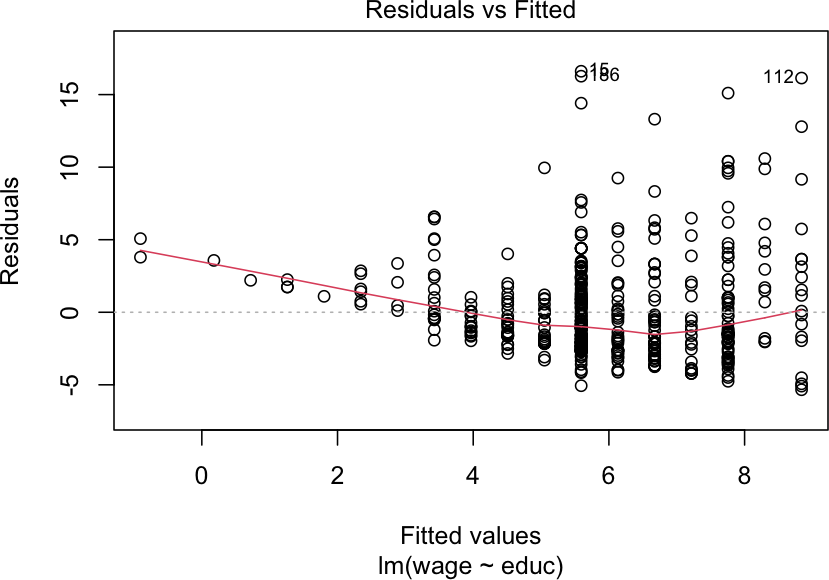
\includegraphics[width=0.8\linewidth]{MEM5220_R_files/figure-latex/fig12-1} 

}

\caption{Regression diagnostics plot base R - Linear Relationship}\label{fig:fig121}
\end{figure}
\begin{figure}

{\centering 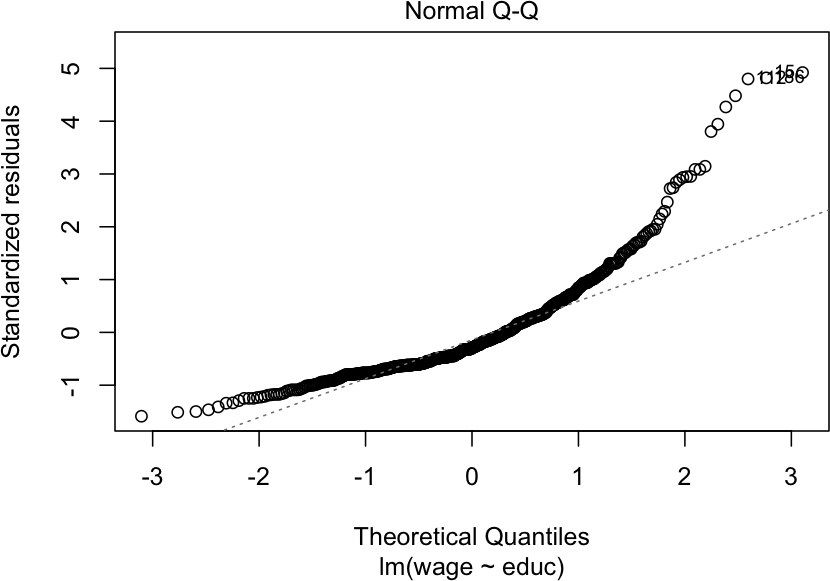
\includegraphics[width=0.8\linewidth]{MEM5220_R_files/figure-latex/fig12-2} 

}

\caption{Regression diagnostics plot base R - Linear Relationship}\label{fig:fig122}
\end{figure}
\begin{figure}

{\centering 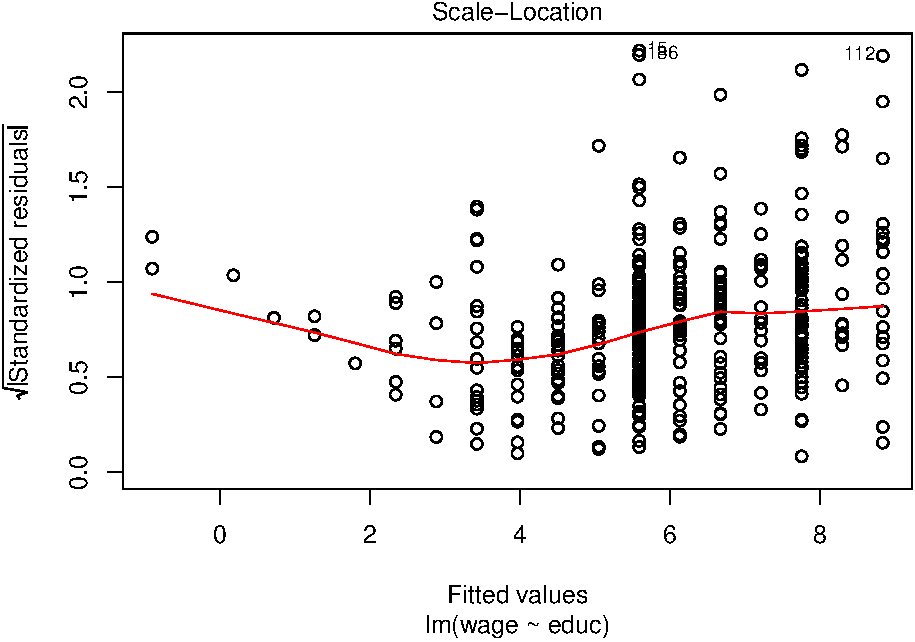
\includegraphics[width=0.8\linewidth]{MEM5220_R_files/figure-latex/fig12-3} 

}

\caption{Regression diagnostics plot base R - Linear Relationship}\label{fig:fig123}
\end{figure}
\begin{figure}

{\centering 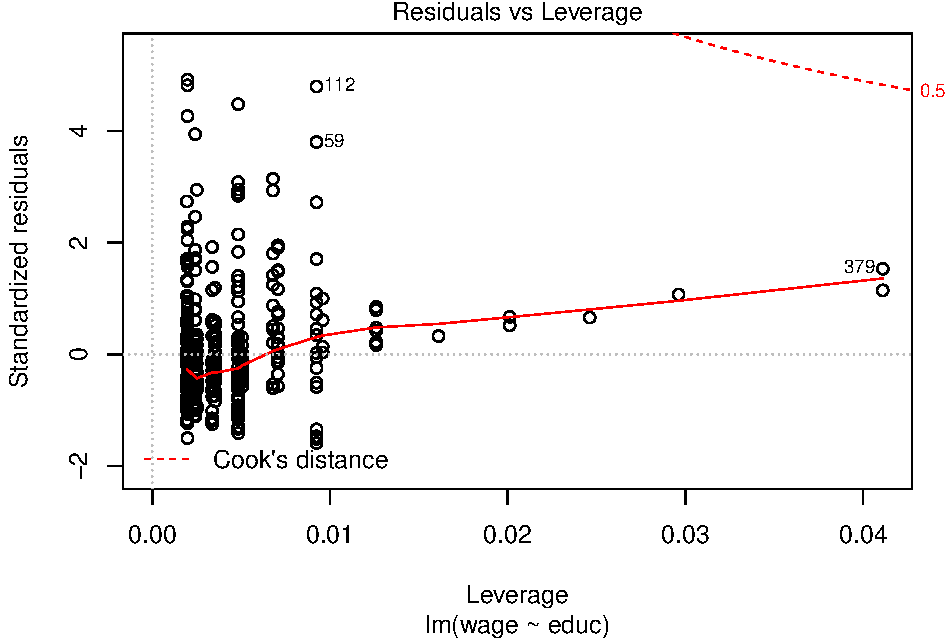
\includegraphics[width=0.8\linewidth]{MEM5220_R_files/figure-latex/fig12-4} 

}

\caption{Regression diagnostics plot base R - Linear Relationship}\label{fig:fig124}
\end{figure}

\begin{Shaded}
\begin{Highlighting}[]
\KeywordTok{autoplot}\NormalTok{(lm_wage, }\DataTypeTok{which =} \DecValTok{1}\OperatorTok{:}\DecValTok{6}\NormalTok{, }\DataTypeTok{colour =} \StringTok{'dodgerblue3'}\NormalTok{,}
         \DataTypeTok{smooth.colour =} \StringTok{'red'}\NormalTok{, }\DataTypeTok{smooth.linetype =} \StringTok{'dashed'}\NormalTok{,}
         \DataTypeTok{ad.colour =} \StringTok{'blue'}\NormalTok{,}
         \DataTypeTok{label =} \OtherTok{FALSE}\NormalTok{,}
         \DataTypeTok{label.size =} \DecValTok{3}\NormalTok{, }\DataTypeTok{label.n =} \DecValTok{5}\NormalTok{, }\DataTypeTok{label.colour =} \StringTok{'blue'}\NormalTok{,}
         \DataTypeTok{ncol =} \DecValTok{3}\NormalTok{) }\OperatorTok{+}
\StringTok{  }\KeywordTok{theme_bw}\NormalTok{()}
\end{Highlighting}
\end{Shaded}

\begin{figure}

{\centering 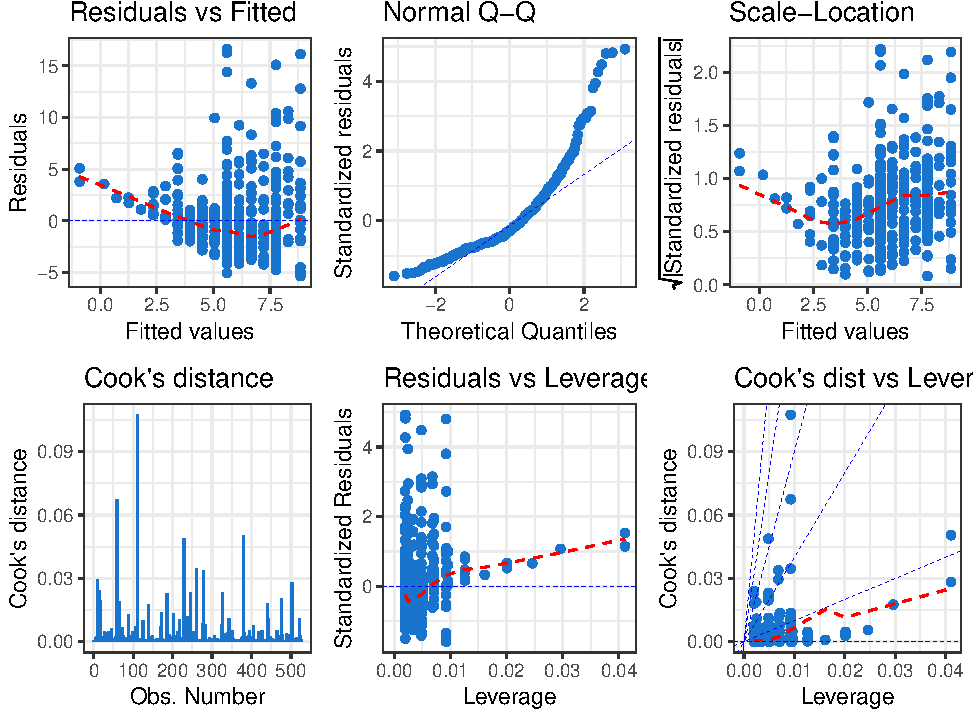
\includegraphics[width=0.8\linewidth]{MEM5220_R_files/figure-latex/fig13-1} 

}

\caption{Regression diagnostics autoplot(ggplot) - Linear Relationship}\label{fig:fig13}
\end{figure}

\begin{Shaded}
\begin{Highlighting}[]
\KeywordTok{autoplot}\NormalTok{(lm_wage1, }\DataTypeTok{which =} \DecValTok{1}\OperatorTok{:}\DecValTok{6}\NormalTok{, }\DataTypeTok{colour =} \StringTok{'dodgerblue3'}\NormalTok{,}
         \DataTypeTok{smooth.colour =} \StringTok{'red'}\NormalTok{, }\DataTypeTok{smooth.linetype =} \StringTok{'dashed'}\NormalTok{,}
         \DataTypeTok{ad.colour =} \StringTok{'blue'}\NormalTok{,}
         \DataTypeTok{label =} \OtherTok{FALSE}\NormalTok{,}
         \DataTypeTok{label.size =} \DecValTok{3}\NormalTok{, }\DataTypeTok{label.n =} \DecValTok{5}\NormalTok{, }\DataTypeTok{label.colour =} \StringTok{'blue'}\NormalTok{,}
         \DataTypeTok{ncol =} \DecValTok{3}\NormalTok{) }\OperatorTok{+}
\StringTok{  }\KeywordTok{theme_bw}\NormalTok{()}
\end{Highlighting}
\end{Shaded}

\begin{figure}

{\centering 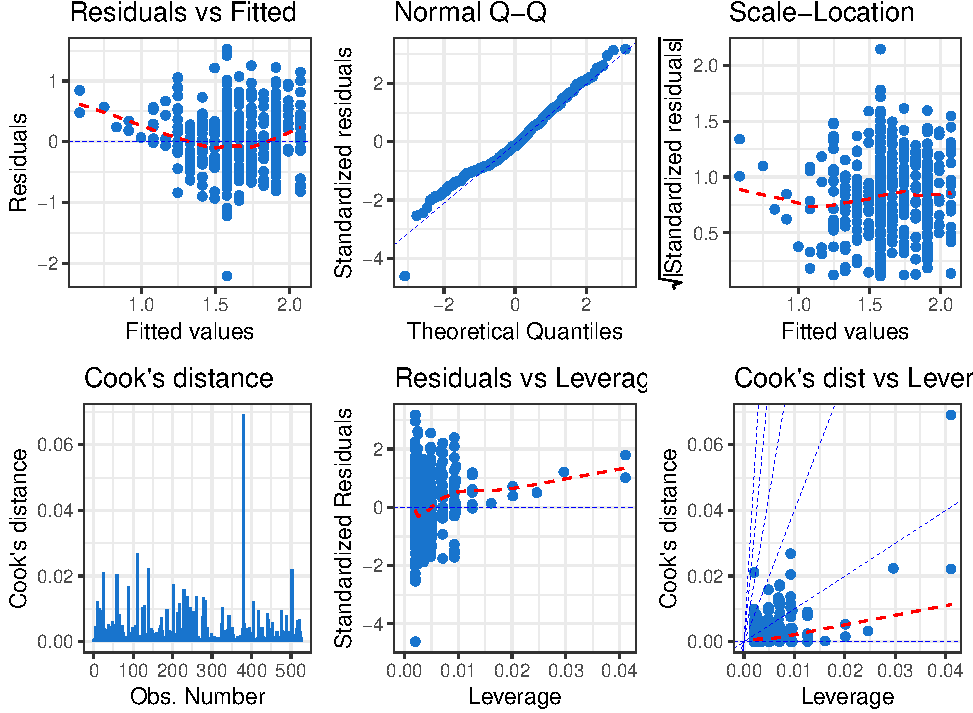
\includegraphics[width=0.8\linewidth]{MEM5220_R_files/figure-latex/fig14-1} 

}

\caption{Regression diagnostics - Non-Linear Relationship}\label{fig:fig14}
\end{figure}

\begin{Shaded}
\begin{Highlighting}[]
\NormalTok{p1_nonlinearities <-}\StringTok{ }\KeywordTok{ggplot}\NormalTok{(wage1, }\KeywordTok{aes}\NormalTok{(}\DataTypeTok{x =}\NormalTok{ educ, }\DataTypeTok{y =}\NormalTok{ wage )) }\OperatorTok{+}
\StringTok{  }\KeywordTok{geom_point}\NormalTok{()   }\OperatorTok{+}\StringTok{ }
\StringTok{  }\KeywordTok{scale_y_continuous}\NormalTok{(}\DataTypeTok{trans=}\StringTok{'log2'}\NormalTok{, }\StringTok{"Log Wage"}\NormalTok{) }\OperatorTok{+}\StringTok{ }
\StringTok{  }\KeywordTok{stat_smooth}\NormalTok{(}\KeywordTok{aes}\NormalTok{(}\DataTypeTok{fill=}\StringTok{"Linear Model"}\NormalTok{),}\DataTypeTok{size=}\DecValTok{1}\NormalTok{,}\DataTypeTok{method =} \StringTok{"lm"}\NormalTok{ ,}\DataTypeTok{span =}\FloatTok{0.3}\NormalTok{, }\DataTypeTok{se=}\NormalTok{F) }\OperatorTok{+}\StringTok{ }
\StringTok{  }\KeywordTok{guides}\NormalTok{(}\DataTypeTok{fill =} \KeywordTok{guide_legend}\NormalTok{(}\StringTok{"Model Type"}\NormalTok{)) }\OperatorTok{+}\StringTok{ }
\StringTok{  }\KeywordTok{theme_bw}\NormalTok{()}
\NormalTok{p1_nonlinearities}
\end{Highlighting}
\end{Shaded}

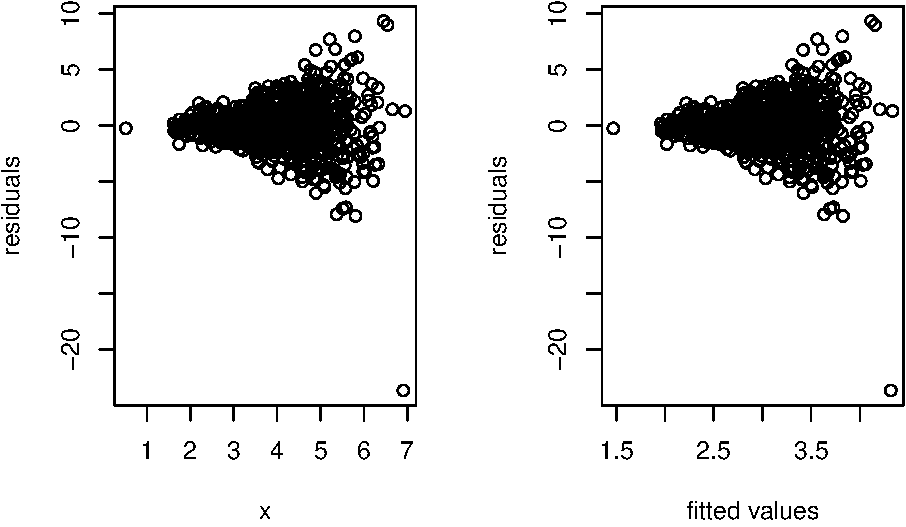
\includegraphics{MEM5220_R_files/figure-latex/unnamed-chunk-55-1.pdf}

Note that if we re-scale the model from a log scale back to the original
scale of the data, we now have

\begin{equation}
Y_{i} = exp(\beta_{0} + \beta_{1} \times x_{i})  \times exp(\epsilon_{i})
\end{equation}

which has errors entering in a multiplicative fashion.

\begin{Shaded}
\begin{Highlighting}[]
\NormalTok{log.model.df <-}\StringTok{ }\KeywordTok{data.frame}\NormalTok{(}\DataTypeTok{x =}\NormalTok{ wage1}\OperatorTok{$}\NormalTok{educ,}
                           \DataTypeTok{y =} \KeywordTok{exp}\NormalTok{(}\KeywordTok{fitted}\NormalTok{(lm_wage1))) }\CommentTok{# This is essentially exp(b0_wage1 + b1_wage1 * wage1$educ) }
\end{Highlighting}
\end{Shaded}

\begin{Shaded}
\begin{Highlighting}[]
\NormalTok{p2_nonlinearities <-}\StringTok{ }\KeywordTok{ggplot}\NormalTok{(wage1, }\KeywordTok{aes}\NormalTok{(}\DataTypeTok{x =}\NormalTok{ educ, }\DataTypeTok{y =}\NormalTok{ wage))  }\OperatorTok{+}
\StringTok{  }\KeywordTok{geom_point}\NormalTok{()   }\OperatorTok{+}
\StringTok{  }\KeywordTok{geom_line}\NormalTok{(}\DataTypeTok{data =}\NormalTok{ log.model.df, }\KeywordTok{aes}\NormalTok{(x, y, }\DataTypeTok{color =} \StringTok{"Log Model"}\NormalTok{), }\DataTypeTok{size =} \DecValTok{1}\NormalTok{, }\DataTypeTok{linetype =} \DecValTok{2}\NormalTok{)  }\OperatorTok{+}
\StringTok{  }\KeywordTok{guides}\NormalTok{(}\DataTypeTok{color =} \KeywordTok{guide_legend}\NormalTok{(}\StringTok{"Model Type"}\NormalTok{)) }\OperatorTok{+}\StringTok{ }
\StringTok{  }\KeywordTok{theme_bw}\NormalTok{()}
\end{Highlighting}
\end{Shaded}

\begin{Shaded}
\begin{Highlighting}[]
\KeywordTok{ggarrange}\NormalTok{(p1_nonlinearities, p2_nonlinearities,  }
          \DataTypeTok{labels =} \KeywordTok{c}\NormalTok{(}\StringTok{"A"}\NormalTok{, }\StringTok{"B"}\NormalTok{),}
          \DataTypeTok{ncol =} \DecValTok{2}\NormalTok{, }\DataTypeTok{nrow =} \DecValTok{1}\NormalTok{)}
\end{Highlighting}
\end{Shaded}

\begin{figure}

{\centering 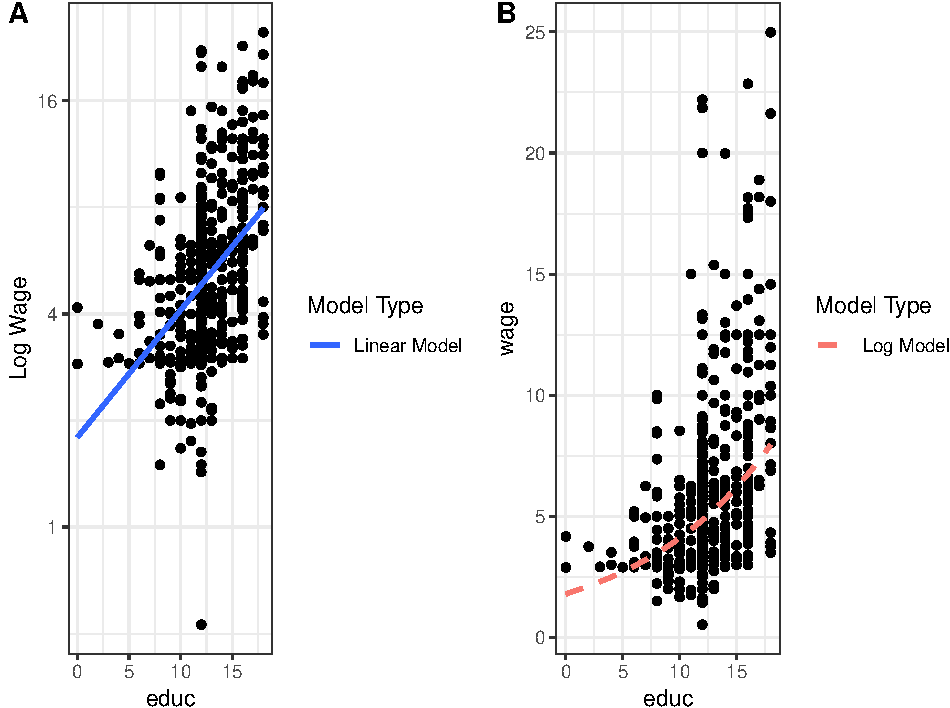
\includegraphics[width=0.8\linewidth]{MEM5220_R_files/figure-latex/fig15-1} 

}

\caption{Wages by Education - Different transformations}\label{fig:fig15}
\end{figure}

A: Plotting the data on the transformed log scale and adding the fitted
line, the relationship again appears linear, and the variation about the
fitted line looks more constant.

B: By plotting the data on the original scale, and adding the fitted
regression, we see an exponential relationship. However, this is still a
\emph{linear} model, since the new transformed response, \(log(Y_{i}\),
is still a \emph{linear} combination of the predictors. In other words,
only \(\beta\) needs to be linear, not the \(x\) values.

\textbf{Quadratic Model}

\begin{equation}
Y_{i} = \beta_{0} + \beta_{1} \times x_{i}  \beta_{2} \times x^2_{i} + \epsilon_{i}
\end{equation}

New dataset from Wooldrige: Collected from the real estate pages of the
Boston Globe during 1990. These are homes that sold in the Boston, MA
area.

\begin{Shaded}
\begin{Highlighting}[]
\KeywordTok{data}\NormalTok{(}\StringTok{"hprice1"}\NormalTok{, }\DataTypeTok{package =} \StringTok{"wooldridge"}\NormalTok{)}
\end{Highlighting}
\end{Shaded}

In R, independent variables involving mathematical operators can be
included in regression equation with the function \texttt{I()}

We estimate the following regression:

\begin{equation}
hprice ~ \beta_{0} +   \beta_{1} sqrft + u
\end{equation}

\begin{Shaded}
\begin{Highlighting}[]
\NormalTok{lm_hprice <-}\StringTok{ }\KeywordTok{lm}\NormalTok{(price }\OperatorTok{~}\StringTok{ }\NormalTok{sqrft, }\DataTypeTok{data  =}\NormalTok{ hprice1)}
\end{Highlighting}
\end{Shaded}

and a regression model that includes a squared term

\begin{equation}
hprice ~ \beta_{0} +   \beta_{1} sqrft + \beta_{2} sqrft^2 + u  
\end{equation}

\begin{Shaded}
\begin{Highlighting}[]
\NormalTok{lm_hprice1 <-}\StringTok{ }\KeywordTok{lm}\NormalTok{(price }\OperatorTok{~}\StringTok{ }\NormalTok{sqrft }\OperatorTok{+}\StringTok{ }\KeywordTok{I}\NormalTok{(sqrft}\OperatorTok{^}\DecValTok{2}\NormalTok{), }\DataTypeTok{data  =}\NormalTok{ hprice1)}
\end{Highlighting}
\end{Shaded}

Alternatively use the \texttt{poly()} function. Be careful of the
additional argument \texttt{raw}.

\begin{Shaded}
\begin{Highlighting}[]
\NormalTok{lm_hprice2 <-}\StringTok{ }\KeywordTok{lm}\NormalTok{(price }\OperatorTok{~}\StringTok{ }\KeywordTok{poly}\NormalTok{(sqrft, }\DataTypeTok{degree =} \DecValTok{2}\NormalTok{),  }\DataTypeTok{data  =}\NormalTok{ hprice1) }
\NormalTok{lm_hprice3 <-}\StringTok{ }\KeywordTok{lm}\NormalTok{(price }\OperatorTok{~}\StringTok{ }\KeywordTok{poly}\NormalTok{(sqrft, }\DataTypeTok{degree =} \DecValTok{2}\NormalTok{, }\DataTypeTok{raw =} \OtherTok{TRUE}\NormalTok{),  }\DataTypeTok{data  =}\NormalTok{ hprice1) }\CommentTok{# if true, use raw and not orthogonal polynomials.}
\end{Highlighting}
\end{Shaded}

\begin{Shaded}
\begin{Highlighting}[]
\KeywordTok{unname}\NormalTok{(}\KeywordTok{coef}\NormalTok{(lm_hprice1))}
\end{Highlighting}
\end{Shaded}

\begin{verbatim}
## [1]  1.849453e+02 -1.710855e-02  3.262809e-05
\end{verbatim}

\begin{Shaded}
\begin{Highlighting}[]
\KeywordTok{unname}\NormalTok{(}\KeywordTok{coef}\NormalTok{(lm_hprice2))}
\end{Highlighting}
\end{Shaded}

\begin{verbatim}
## [1] 293.5460 754.8517 135.6051
\end{verbatim}

\begin{Shaded}
\begin{Highlighting}[]
\KeywordTok{unname}\NormalTok{(}\KeywordTok{coef}\NormalTok{(lm_hprice3))}
\end{Highlighting}
\end{Shaded}

\begin{verbatim}
## [1]  1.849453e+02 -1.710855e-02  3.262809e-05
\end{verbatim}

\begin{Shaded}
\begin{Highlighting}[]
\KeywordTok{all.equal}\NormalTok{(}\KeywordTok{unname}\NormalTok{(}\KeywordTok{coef}\NormalTok{(lm_hprice1)), }\KeywordTok{unname}\NormalTok{(}\KeywordTok{coef}\NormalTok{(lm_hprice2)))}
\end{Highlighting}
\end{Shaded}

\begin{verbatim}
## [1] "Mean relative difference: 5.401501"
\end{verbatim}

\begin{Shaded}
\begin{Highlighting}[]
\KeywordTok{all.equal}\NormalTok{(}\KeywordTok{unname}\NormalTok{(}\KeywordTok{coef}\NormalTok{(lm_hprice1)), }\KeywordTok{unname}\NormalTok{(}\KeywordTok{coef}\NormalTok{(lm_hprice3)))}
\end{Highlighting}
\end{Shaded}

\begin{verbatim}
## [1] TRUE
\end{verbatim}

\begin{Shaded}
\begin{Highlighting}[]
\KeywordTok{all.equal}\NormalTok{(}\KeywordTok{fitted}\NormalTok{(lm_hprice1), }\KeywordTok{fitted}\NormalTok{(lm_hprice2))}
\end{Highlighting}
\end{Shaded}

\begin{verbatim}
## [1] TRUE
\end{verbatim}

\begin{Shaded}
\begin{Highlighting}[]
\KeywordTok{all.equal}\NormalTok{(}\KeywordTok{fitted}\NormalTok{(lm_hprice1), }\KeywordTok{fitted}\NormalTok{(lm_hprice3))}
\end{Highlighting}
\end{Shaded}

\begin{verbatim}
## [1] TRUE
\end{verbatim}

With the function \texttt{all.equal()} we can test if all elements in
two vectors are the ``nearly'' the same. ``Nearly'' refers to the case
when \emph{tolerance} values are exceeded.

Why are those values not the same depending on the \texttt{poly()}
function argument \texttt{raw\ =\ True}? In the case of
\texttt{raw\ =\ True} R uses raw and not orthogonal polynomials.

This can have importan implications in the case when multiple
polynimoals are used in the regression. The linear regressar \(sqrft\)
is uncorrelated linearly with the squared explanatory variable
\(sqrft^2\). However, if we add a cubic term \(sqrft^3\),
multicollinearty between \(sqrft^2\) and \(sqrft^3\) might become and
issues of the polynomials are \emph{NOT} orthogonalized.

We can also extract the standard error of our estimated coefficents
manually.

Starting with the variance-covariance matrix of the regression model

\begin{Shaded}
\begin{Highlighting}[]
\NormalTok{vcov_lm_hprice2 <-}\StringTok{ }\KeywordTok{vcov}\NormalTok{(lm_hprice2)}
\end{Highlighting}
\end{Shaded}

Extracting only the diagonal element of the matrix and taking the square
root we obtain the standard errors as reported in \texttt{summary()}
function call.

\begin{Shaded}
\begin{Highlighting}[]
\KeywordTok{sqrt}\NormalTok{(}\KeywordTok{diag}\NormalTok{(vcov_lm_hprice2))}
\end{Highlighting}
\end{Shaded}

\begin{verbatim}
##              (Intercept) poly(sqrft, degree = 2)1 poly(sqrft, degree = 2)2 
##                 6.638736                62.276866                62.276866
\end{verbatim}

\begin{Shaded}
\begin{Highlighting}[]
\KeywordTok{summary}\NormalTok{(lm_hprice2)}
\end{Highlighting}
\end{Shaded}

\begin{verbatim}
## 
## Call:
## lm(formula = price ~ poly(sqrft, degree = 2), data = hprice1)
## 
## Residuals:
##      Min       1Q   Median       3Q      Max 
## -158.261  -35.158   -7.924   24.262  223.516 
## 
## Coefficients:
##                          Estimate Std. Error t value Pr(>|t|)    
## (Intercept)               293.546      6.639  44.217   <2e-16 ***
## poly(sqrft, degree = 2)1  754.852     62.277  12.121   <2e-16 ***
## poly(sqrft, degree = 2)2  135.605     62.277   2.177   0.0322 *  
## ---
## Signif. codes:  0 '***' 0.001 '**' 0.01 '*' 0.05 '.' 0.1 ' ' 1
## 
## Residual standard error: 62.28 on 85 degrees of freedom
## Multiple R-squared:  0.6408, Adjusted R-squared:  0.6324 
## F-statistic: 75.83 on 2 and 85 DF,  p-value: < 2.2e-16
\end{verbatim}

\hypertarget{multiple-linear-regression}{%
\section{Multiple Linear Regression}\label{multiple-linear-regression}}

\begin{center}\rule{0.5\linewidth}{\linethickness}\end{center}

\textbf{Note}

A \textbf{(general) linear model} is similar to the simple variant, but
with a multivariate \(x \epsilon \!R^{\rho}\) and a mean given by a
hyperplane in place of a single line.

\begin{itemize}
\tightlist
\item
  General principles are the same as the simple case
\item
  Math is more difficult because we need to use matrices
\item
  Interpretation is more difficult because the \(\beta_{j}\) are effects
  conditional on the other variables
\end{itemize}

Many would retain the same signs as the simple linear regression, but
the magnitudes would be smaller. In some cases, it is possible for the
relationship to flip directions when a second (highly correlated)
variable is added \citet{dalpiaz2016}.

\begin{center}\rule{0.5\linewidth}{\linethickness}\end{center}

\begin{equation}
y = \beta_{0} + \beta_{1}x_{1} +  \beta_{2}x_{2} + \dots + \beta_{k}x_{k} + u   
\label{eq:multipleregression}
\end{equation}

The next example from Wooldrige relates the college GPA (``cloGPA'') to
the high school GPA (``hsGPA'') and achievement test score (``ACT'') for
a sample of 141 students.

\begin{Shaded}
\begin{Highlighting}[]
\KeywordTok{data}\NormalTok{(}\StringTok{"gpa1"}\NormalTok{, }\DataTypeTok{package =} \StringTok{"wooldridge"}\NormalTok{)}
\KeywordTok{attach}\NormalTok{(gpa1)}
\end{Highlighting}
\end{Shaded}

\begin{verbatim}
## The following object is masked from package:robustbase:
## 
##     alcohol
\end{verbatim}

\begin{verbatim}
## The following objects are masked from package:wooldridge:
## 
##     alcohol, campus
\end{verbatim}

\begin{Shaded}
\begin{Highlighting}[]
\NormalTok{?gpa1}
\end{Highlighting}
\end{Shaded}

Obtain parameter estimates

\begin{Shaded}
\begin{Highlighting}[]
\NormalTok{GPAres <-}\StringTok{ }\KeywordTok{lm}\NormalTok{(colGPA }\OperatorTok{~}\StringTok{ }\NormalTok{hsGPA }\OperatorTok{+}\StringTok{ }\NormalTok{ACT, }\DataTypeTok{data =}\NormalTok{ gpa1)}
\KeywordTok{summary}\NormalTok{(GPAres)}
\end{Highlighting}
\end{Shaded}

\begin{verbatim}
## 
## Call:
## lm(formula = colGPA ~ hsGPA + ACT, data = gpa1)
## 
## Residuals:
##      Min       1Q   Median       3Q      Max 
## -0.85442 -0.24666 -0.02614  0.28127  0.85357 
## 
## Coefficients:
##             Estimate Std. Error t value Pr(>|t|)    
## (Intercept) 1.286328   0.340822   3.774 0.000238 ***
## hsGPA       0.453456   0.095813   4.733 5.42e-06 ***
## ACT         0.009426   0.010777   0.875 0.383297    
## ---
## Signif. codes:  0 '***' 0.001 '**' 0.01 '*' 0.05 '.' 0.1 ' ' 1
## 
## Residual standard error: 0.3403 on 138 degrees of freedom
## Multiple R-squared:  0.1764, Adjusted R-squared:  0.1645 
## F-statistic: 14.78 on 2 and 138 DF,  p-value: 1.526e-06
\end{verbatim}

\begin{Shaded}
\begin{Highlighting}[]
\KeywordTok{coef}\NormalTok{(GPAres)[[}\DecValTok{1}\NormalTok{]]}
\end{Highlighting}
\end{Shaded}

\begin{verbatim}
## [1] 1.286328
\end{verbatim}

In the multiple linear regression setting, some of the interpretations
of the coefficients change slightly. Here, \(\hat\beta_{0} =\) 1.2863278
is our estimate for \(\beta_{0}\) when all of the predictors are 0. In
this example this makes sense but think of the following example:

\begin{center}\rule{0.5\linewidth}{\linethickness}\end{center}

\textbf{Your turn}

Assume the following model:

\begin{Shaded}
\begin{Highlighting}[]
\NormalTok{mpg_model =}\StringTok{ }\KeywordTok{lm}\NormalTok{(hp }\OperatorTok{~}\StringTok{ }\NormalTok{wt }\OperatorTok{+}\StringTok{ }\NormalTok{cyl, }\DataTypeTok{data =}\NormalTok{ mtcars)}
\KeywordTok{coef}\NormalTok{(mpg_model)}
\end{Highlighting}
\end{Shaded}

\begin{verbatim}
## (Intercept)          wt         cyl 
##  -51.805567    1.330463   31.387901
\end{verbatim}

How do you interpret the intercept coefficient estimate?

A: Here, \(\hat\beta_{0} =\) -51.8055669 is our estimate for
\(\beta_{0}\), the mean gross horsepower for a car that weights 0 pounds
and has 0 cylinders. We see our estimate here is negative, which is a
physical impossibility. However, this isn't unexpected, as we shouldn't
expect our model to be accurate for cars which weight 0 pounds and have
no cylinders to propel the engine.

\begin{center}\rule{0.5\linewidth}{\linethickness}\end{center}

\begin{Shaded}
\begin{Highlighting}[]
\KeywordTok{with}\NormalTok{ (gpa1, \{}
  \CommentTok{# find min-max seq for grid construction}
\NormalTok{  min_hsGPA <-}\StringTok{ }\KeywordTok{min}\NormalTok{(gpa1}\OperatorTok{$}\NormalTok{hsGPA)}
\NormalTok{  max_hsGPA <-}\StringTok{ }\KeywordTok{max}\NormalTok{(gpa1}\OperatorTok{$}\NormalTok{hsGPA)}
\NormalTok{  min_ACT <-}\StringTok{ }\KeywordTok{min}\NormalTok{(gpa1}\OperatorTok{$}\NormalTok{ACT)}
\NormalTok{  max_ACT <-}\StringTok{ }\KeywordTok{max}\NormalTok{(gpa1}\OperatorTok{$}\NormalTok{ACT)}
  
  
  \CommentTok{# linear regression}
\NormalTok{  fit <-}\StringTok{ }\KeywordTok{lm}\NormalTok{(colGPA }\OperatorTok{~}\StringTok{ }\NormalTok{hsGPA }\OperatorTok{+}\StringTok{ }\NormalTok{ACT)}
  
  \CommentTok{# predict values on regular xy grid}
\NormalTok{  hsGPA.pred <-}\StringTok{ }\KeywordTok{seq}\NormalTok{(min_hsGPA, max_hsGPA, }\DataTypeTok{length.out =} \DecValTok{30}\NormalTok{)}
\NormalTok{  ACT.pred <-}\StringTok{ }\KeywordTok{seq}\NormalTok{(min_ACT, max_ACT, }\DataTypeTok{length.out =} \DecValTok{30}\NormalTok{)}
\NormalTok{  xy <-}\StringTok{ }\KeywordTok{expand.grid}\NormalTok{(}\DataTypeTok{hsGPA =}\NormalTok{ hsGPA.pred, }
                    \DataTypeTok{ACT =}\NormalTok{ ACT.pred)}
  
\NormalTok{  colGPA.pred <-}\StringTok{ }\KeywordTok{matrix}\NormalTok{ (}\DataTypeTok{nrow =} \DecValTok{30}\NormalTok{, }\DataTypeTok{ncol =} \DecValTok{30}\NormalTok{, }
                         \DataTypeTok{data =} \KeywordTok{predict}\NormalTok{(fit, }\DataTypeTok{newdata =} \KeywordTok{data.frame}\NormalTok{(xy), }
                                        \DataTypeTok{interval =} \StringTok{"prediction"}\NormalTok{))}
  
  \CommentTok{# fitted points for droplines to surface}
\NormalTok{  fitpoints <-}\StringTok{ }\KeywordTok{predict}\NormalTok{(fit) }
  
  \KeywordTok{scatter3D}\NormalTok{(}\DataTypeTok{z =}\NormalTok{ colGPA, }\DataTypeTok{x =}\NormalTok{ hsGPA, }\DataTypeTok{y =}\NormalTok{ ACT, }\DataTypeTok{pch =} \DecValTok{18}\NormalTok{, }\DataTypeTok{cex =} \DecValTok{2}\NormalTok{, }
            \DataTypeTok{theta =} \DecValTok{20}\NormalTok{, }\DataTypeTok{phi =} \DecValTok{20}\NormalTok{, }\DataTypeTok{ticktype =} \StringTok{"detailed"}\NormalTok{,}
            \DataTypeTok{xlab =} \StringTok{"hsGPA"}\NormalTok{, }\DataTypeTok{ylab =} \StringTok{"ACT"}\NormalTok{, }\DataTypeTok{zlab =} \StringTok{"colGPA"}\NormalTok{,  }
            \DataTypeTok{surf =} \KeywordTok{list}\NormalTok{(}\DataTypeTok{x =}\NormalTok{ hsGPA.pred, }\DataTypeTok{y =}\NormalTok{ ACT.pred, }\DataTypeTok{z =}\NormalTok{ colGPA.pred,  }
                        \DataTypeTok{facets =} \OtherTok{NA}\NormalTok{, }\DataTypeTok{fit =}\NormalTok{ fitpoints),}
            \DataTypeTok{main =} \StringTok{"colGPA"}\NormalTok{)}
  
\NormalTok{\})}
\end{Highlighting}
\end{Shaded}

\begin{figure}

{\centering 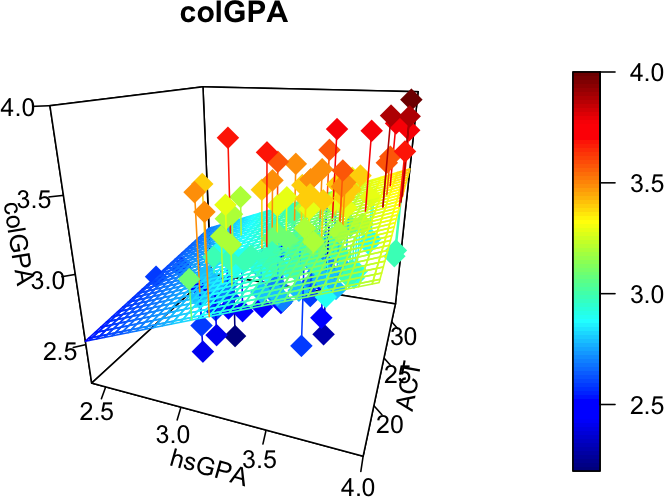
\includegraphics[width=0.8\linewidth]{MEM5220_R_files/figure-latex/fig16-1} 

}

\caption{College GPA  High School GPA + Achievment test score}\label{fig:fig16}
\end{figure}

The data points (\(x_{i1}\),\(x_{i2}\),\(y_{i}\)) now exist in
3-dimensional space, so instead of fitting a line to the data, we will
fit a plane.

\hypertarget{ceteris-paribus-interpretation-and-omitted-variable-bias}{%
\subsection{Ceteris Paribus Interpretation and Omitted Variable
bias}\label{ceteris-paribus-interpretation-and-omitted-variable-bias}}

Consider a regression with two explanatory variables

\begin{equation}
\hat{y} = \hat{\beta}_{0} + \hat{\beta}_{1}x_{1} +  \hat{\beta}_{2}x_{2}    
\label{eq:lmtwoexplanatory}
\end{equation}

\begin{Shaded}
\begin{Highlighting}[]
\CommentTok{# Parameter estimates for full and simple model:}
\NormalTok{beta.hat <-}\StringTok{ }\KeywordTok{coef}\NormalTok{( }\KeywordTok{lm}\NormalTok{(colGPA }\OperatorTok{~}\StringTok{ }\NormalTok{ACT}\OperatorTok{+}\NormalTok{hsGPA, }\DataTypeTok{data=}\NormalTok{gpa1))}
\NormalTok{beta.hat}
\end{Highlighting}
\end{Shaded}

\begin{verbatim}
## (Intercept)         ACT       hsGPA 
## 1.286327767 0.009426012 0.453455885
\end{verbatim}

Now, lets omit one variable in the regression

\begin{equation}
\hat{y} = \hat{\beta}_{0} + \hat{\beta}_{1}x_{1}    
\label{eq:lmomitted}
\end{equation}

\begin{Shaded}
\begin{Highlighting}[]
\CommentTok{# Relation between regressors:}
\NormalTok{delta.tilde <-}\StringTok{ }\KeywordTok{coef}\NormalTok{( }\KeywordTok{lm}\NormalTok{(hsGPA }\OperatorTok{~}\StringTok{ }\NormalTok{ACT, }\DataTypeTok{data=}\NormalTok{gpa1) )}
\NormalTok{delta.tilde}
\end{Highlighting}
\end{Shaded}

\begin{verbatim}
## (Intercept)         ACT 
##  2.46253658  0.03889675
\end{verbatim}

The parameter \(\hat\beta_1\) is the estimated effect of increasing
\(x_1\) by one unit (and \textbf{NOT} keeping \(x_2\) fixed). It can be
related to \(\hat\beta_1\) using the formula

\begin{equation}
\hat{y} = \hat{\beta}_{0} + \hat{\beta}_{1} x_{1} +  \hat{\beta}_{2}  \tilde\delta_{1}
\label{eq:lmommited}
\end{equation}

where \(\tilde\delta_{1}\) is the slope parameters of the linear
regression of \(x_2\) on \(x_1\)

\begin{equation}
\hat{x}_2 = \tilde\delta_{0} + \tilde\delta_{1} x_{1}
\label{eq:lmomitted2}
\end{equation}

\begin{Shaded}
\begin{Highlighting}[]
\CommentTok{# Omitted variables formula for beta1.tilde:}
\NormalTok{beta.hat[}\StringTok{"ACT"}\NormalTok{] }\OperatorTok{+}\StringTok{ }\NormalTok{beta.hat[}\StringTok{"hsGPA"}\NormalTok{]}\OperatorTok{*}\NormalTok{delta.tilde[}\StringTok{"ACT"}\NormalTok{]}
\end{Highlighting}
\end{Shaded}

\begin{verbatim}
##        ACT 
## 0.02706397
\end{verbatim}

\begin{Shaded}
\begin{Highlighting}[]
\CommentTok{# Actual regression with hsGPA omitted:}
\KeywordTok{summary}\NormalTok{(}\KeywordTok{lm}\NormalTok{(colGPA }\OperatorTok{~}\StringTok{ }\NormalTok{ACT, }\DataTypeTok{data=}\NormalTok{gpa1))}
\end{Highlighting}
\end{Shaded}

\begin{verbatim}
## 
## Call:
## lm(formula = colGPA ~ ACT, data = gpa1)
## 
## Residuals:
##      Min       1Q   Median       3Q      Max 
## -0.85251 -0.25251 -0.04426  0.26400  0.89336 
## 
## Coefficients:
##             Estimate Std. Error t value Pr(>|t|)    
## (Intercept)  2.40298    0.26420   9.095  8.8e-16 ***
## ACT          0.02706    0.01086   2.491   0.0139 *  
## ---
## Signif. codes:  0 '***' 0.001 '**' 0.01 '*' 0.05 '.' 0.1 ' ' 1
## 
## Residual standard error: 0.3656 on 139 degrees of freedom
## Multiple R-squared:  0.04275,    Adjusted R-squared:  0.03586 
## F-statistic: 6.207 on 1 and 139 DF,  p-value: 0.0139
\end{verbatim}

In this example, the indirect effect is actually stronger than the
direct effect. \emph{ACT} predicts \emph{colGPA} mainly because it is
related to \emph{hsGPA} which in turn is strongly related to
\emph{colGPA}.

\hypertarget{standard-errors-multicollinearity-and-vif}{%
\subsection{Standard errors, Multicollinearity and
VIF}\label{standard-errors-multicollinearity-and-vif}}

Multicollinearity means that two or more regressors in a multiple
regression model are strongly correlated. If the correlation between two
or more regressors is perfect, that is, one regressor can be written as
a linear combination of the other(s), we have perfect multicollinearity.
While strong multicollinearity in general is unpleasant as it causes the
variance of the OLS estimator to be large (we will discuss this in more
detail later), the presence of perfect multicollinearity makes it
impossible to solve for the OLS estimator, i.e., the model cannot be
estimated in the first place.

\hypertarget{perfect-multicollinearity}{%
\subsubsection{Perfect
multicollinearity}\label{perfect-multicollinearity}}

We will work first with the \emph{CAschools} data from the \textbf{AER}
package to simulate an example of perfect multicollinearity

\begin{Shaded}
\begin{Highlighting}[]
\KeywordTok{data}\NormalTok{(}\StringTok{"CASchools"}\NormalTok{, }\DataTypeTok{package =} \StringTok{"AER"}\NormalTok{)}
\NormalTok{?CASchools}
\end{Highlighting}
\end{Shaded}

\begin{Shaded}
\begin{Highlighting}[]
\CommentTok{# define the fraction of English learners        }
\NormalTok{CASchools}\OperatorTok{$}\NormalTok{FracEL <-}\StringTok{ }\NormalTok{CASchools}\OperatorTok{$}\NormalTok{english }\OperatorTok{/}\StringTok{ }\DecValTok{100}

\CommentTok{# check the correlation between CASchools$FracEL and CASchools$english }
\KeywordTok{cor}\NormalTok{(CASchools}\OperatorTok{$}\NormalTok{FracEL, CASchools}\OperatorTok{$}\NormalTok{english)}
\end{Highlighting}
\end{Shaded}

\begin{verbatim}
## [1] 1
\end{verbatim}

\begin{Shaded}
\begin{Highlighting}[]
\CommentTok{# estimate the model}
\NormalTok{mult.mod <-}\StringTok{ }\KeywordTok{lm}\NormalTok{(read }\OperatorTok{~}\StringTok{ }\NormalTok{students }\OperatorTok{+}\StringTok{ }\NormalTok{english }\OperatorTok{+}\StringTok{ }\NormalTok{FracEL, }\DataTypeTok{data =}\NormalTok{ CASchools) }

\CommentTok{# obtain a summary of the model}
\KeywordTok{summary}\NormalTok{(mult.mod)  }
\end{Highlighting}
\end{Shaded}

\begin{verbatim}
## 
## Call:
## lm(formula = read ~ students + english + FracEL, data = CASchools)
## 
## Residuals:
##     Min      1Q  Median      3Q     Max 
## -51.077  -9.767  -0.695   9.097  40.005 
## 
## Coefficients: (1 not defined because of singularities)
##               Estimate Std. Error t value Pr(>|t|)    
## (Intercept)  6.665e+02  9.771e-01 682.054   <2e-16 ***
## students     3.326e-04  1.941e-04   1.714   0.0873 .  
## english     -7.843e-01  4.153e-02 -18.886   <2e-16 ***
## FracEL              NA         NA      NA       NA    
## ---
## Signif. codes:  0 '***' 0.001 '**' 0.01 '*' 0.05 '.' 0.1 ' ' 1
## 
## Residual standard error: 14.53 on 417 degrees of freedom
## Multiple R-squared:  0.4802, Adjusted R-squared:  0.4777 
## F-statistic: 192.6 on 2 and 417 DF,  p-value: < 2.2e-16
\end{verbatim}

The row \emph{FracEL} in the coefficients section of the output consists
of NA entries since FracEL was excluded from the model.

Another example of perfect multicollinearity is known as the dummy
variable trap. This may occur when multiple dummy variables are used as
regressors. A common case for this is when dummies are used to sort the
data into mutually exclusive categories. For example, suppose we have
spatial information that indicates whether a school is located in the
North, West, South or East of California.

\begin{Shaded}
\begin{Highlighting}[]
\CommentTok{# set seed for reproducibility}
\KeywordTok{set.seed}\NormalTok{(}\DecValTok{1}\NormalTok{)}

\CommentTok{# generate artificial data on location}
\NormalTok{CASchools}\OperatorTok{$}\NormalTok{direction <-}\StringTok{ }\KeywordTok{sample}\NormalTok{(}\KeywordTok{c}\NormalTok{(}\StringTok{"West"}\NormalTok{, }\StringTok{"North"}\NormalTok{, }\StringTok{"South"}\NormalTok{, }\StringTok{"East"}\NormalTok{), }
                              \DecValTok{420}\NormalTok{, }
                              \DataTypeTok{replace =}\NormalTok{ T)}

\CommentTok{# estimate the model}
\NormalTok{mult.mod <-}\StringTok{ }\KeywordTok{lm}\NormalTok{(read }\OperatorTok{~}\StringTok{ }\NormalTok{students }\OperatorTok{+}\StringTok{ }\NormalTok{english }\OperatorTok{+}\StringTok{ }\NormalTok{direction, }\DataTypeTok{data =}\NormalTok{ CASchools)}

\CommentTok{# obtain a model summary}
\KeywordTok{summary}\NormalTok{(mult.mod)   }
\end{Highlighting}
\end{Shaded}

\begin{verbatim}
## 
## Call:
## lm(formula = read ~ students + english + direction, data = CASchools)
## 
## Residuals:
##     Min      1Q  Median      3Q     Max 
## -50.518  -9.690  -1.146   8.926  39.698 
## 
## Coefficients:
##                  Estimate Std. Error t value Pr(>|t|)    
## (Intercept)     6.659e+02  1.547e+00 430.575   <2e-16 ***
## students        3.177e-04  1.945e-04   1.634    0.103    
## english        -7.844e-01  4.154e-02 -18.882   <2e-16 ***
## directionNorth  9.185e-01  1.934e+00   0.475    0.635    
## directionSouth -1.119e+00  2.081e+00  -0.537    0.591    
## directionWest   2.436e+00  2.057e+00   1.184    0.237    
## ---
## Signif. codes:  0 '***' 0.001 '**' 0.01 '*' 0.05 '.' 0.1 ' ' 1
## 
## Residual standard error: 14.53 on 414 degrees of freedom
## Multiple R-squared:  0.484,  Adjusted R-squared:  0.4778 
## F-statistic: 77.67 on 5 and 414 DF,  p-value: < 2.2e-16
\end{verbatim}

Notice that R solves the problem on its own by generating and including
the dummies directionNorth, directionSouth and directionWest but
omitting directionEast. Of course, the omission of every other dummy
instead would achieve the same. Another solution would be to exclude the
constant and to include all dummies instead.

A last example considers the case where a perfect linear relationship
arises from redundant regressors. Suppose we have a regressor\\
Spanish speakers, \emph{spanish}, , the percentage of English speakers
in the school where

\begin{equation}
spanish = 100 - english  
\end{equation}

and both \emph{spanish} and \emph{english} are included in a regression
model.

\begin{Shaded}
\begin{Highlighting}[]
\CommentTok{# Percentage of english speakers }
\NormalTok{CASchools}\OperatorTok{$}\NormalTok{spanish <-}\StringTok{ }\DecValTok{100} \OperatorTok{-}\StringTok{ }\NormalTok{CASchools}\OperatorTok{$}\NormalTok{english}

\CommentTok{# estimate the model}
\NormalTok{mult.mod <-}\StringTok{ }\KeywordTok{lm}\NormalTok{(read }\OperatorTok{~}\StringTok{ }\NormalTok{students }\OperatorTok{+}\StringTok{ }\NormalTok{english }\OperatorTok{+}\StringTok{ }\NormalTok{spanish, }\DataTypeTok{data =}\NormalTok{ CASchools)}

\CommentTok{# obtain a model summary}
\KeywordTok{summary}\NormalTok{(mult.mod)                                                 }
\end{Highlighting}
\end{Shaded}

\begin{verbatim}
## 
## Call:
## lm(formula = read ~ students + english + spanish, data = CASchools)
## 
## Residuals:
##     Min      1Q  Median      3Q     Max 
## -51.077  -9.767  -0.695   9.097  40.005 
## 
## Coefficients: (1 not defined because of singularities)
##               Estimate Std. Error t value Pr(>|t|)    
## (Intercept)  6.665e+02  9.771e-01 682.054   <2e-16 ***
## students     3.326e-04  1.941e-04   1.714   0.0873 .  
## english     -7.843e-01  4.153e-02 -18.886   <2e-16 ***
## spanish             NA         NA      NA       NA    
## ---
## Signif. codes:  0 '***' 0.001 '**' 0.01 '*' 0.05 '.' 0.1 ' ' 1
## 
## Residual standard error: 14.53 on 417 degrees of freedom
## Multiple R-squared:  0.4802, Adjusted R-squared:  0.4777 
## F-statistic: 192.6 on 2 and 417 DF,  p-value: < 2.2e-16
\end{verbatim}

Once more, \texttt{lm()} refuses to estimate the full model using OLS
and excludes spanish.

\hypertarget{imperfect-multicollinearity}{%
\subsubsection{Imperfect
multicollinearity}\label{imperfect-multicollinearity}}

As opposed to perfect multicollinearity, imperfect multicollinearity is
--- to a certain extent --- less of a problem. In fact, imperfect
multicollinearity is the reason why we are interested in estimating
multiple regression models in the first place: the OLS estimator allows
us to isolate influences of correlated regressors on the dependent
variable. If it was not for these dependencies, there would not be a
reason to resort to a multiple regression approach and we could simply
work with a single-regressor model. However, this is rarely the case in
applications. We already know that ignoring dependencies among
regressors which influence the outcome variable has an adverse effect on
estimation results.

Simulation study: imperfect multicollinearity

\begin{Shaded}
\begin{Highlighting}[]
\CommentTok{# set number of observations}
\NormalTok{n <-}\StringTok{ }\DecValTok{50}

\CommentTok{# initialize vectors of coefficients}
\NormalTok{coefs1 <-}\StringTok{ }\KeywordTok{cbind}\NormalTok{(}\StringTok{"hat_beta_1"}\NormalTok{ =}\StringTok{ }\KeywordTok{numeric}\NormalTok{(}\DecValTok{10000}\NormalTok{), }\StringTok{"hat_beta_2"}\NormalTok{ =}\StringTok{ }\KeywordTok{numeric}\NormalTok{(}\DecValTok{10000}\NormalTok{))}
\NormalTok{coefs2 <-}\StringTok{ }\NormalTok{coefs1}

\CommentTok{# set seed}
\KeywordTok{set.seed}\NormalTok{(}\DecValTok{1}\NormalTok{)}

\CommentTok{# loop sampling and estimation}
\ControlFlowTok{for}\NormalTok{ (i }\ControlFlowTok{in} \DecValTok{1}\OperatorTok{:}\DecValTok{1000}\NormalTok{) \{}
  
  \CommentTok{# for cov(X_1,X_2) = 0.25}
\NormalTok{  X <-}\StringTok{ }\KeywordTok{rmvnorm}\NormalTok{(n, }\KeywordTok{c}\NormalTok{(}\DecValTok{50}\NormalTok{, }\DecValTok{100}\NormalTok{), }\DataTypeTok{sigma =} \KeywordTok{cbind}\NormalTok{(}\KeywordTok{c}\NormalTok{(}\DecValTok{10}\NormalTok{, }\FloatTok{2.5}\NormalTok{), }\KeywordTok{c}\NormalTok{(}\FloatTok{2.5}\NormalTok{, }\DecValTok{10}\NormalTok{))) }\CommentTok{# function from the mvtnorm package}
\NormalTok{  u <-}\StringTok{ }\KeywordTok{rnorm}\NormalTok{(n, }\DataTypeTok{sd =} \DecValTok{5}\NormalTok{)}
\NormalTok{  Y <-}\StringTok{ }\DecValTok{5} \OperatorTok{+}\StringTok{ }\FloatTok{2.5} \OperatorTok{*}\StringTok{ }\NormalTok{X[, }\DecValTok{1}\NormalTok{] }\OperatorTok{+}\StringTok{ }\DecValTok{3} \OperatorTok{*}\StringTok{ }\NormalTok{X[, }\DecValTok{2}\NormalTok{] }\OperatorTok{+}\StringTok{ }\NormalTok{u}
\NormalTok{  coefs1[i, ] <-}\StringTok{ }\KeywordTok{lm}\NormalTok{(Y }\OperatorTok{~}\StringTok{ }\NormalTok{X[, }\DecValTok{1}\NormalTok{] }\OperatorTok{+}\StringTok{ }\NormalTok{X[, }\DecValTok{2}\NormalTok{])}\OperatorTok{$}\NormalTok{coefficients[}\OperatorTok{-}\DecValTok{1}\NormalTok{]}
  
  \CommentTok{# for cov(X_1,X_2) = 0.85}
\NormalTok{  X <-}\StringTok{ }\KeywordTok{rmvnorm}\NormalTok{(n, }\KeywordTok{c}\NormalTok{(}\DecValTok{50}\NormalTok{, }\DecValTok{100}\NormalTok{), }\DataTypeTok{sigma =} \KeywordTok{cbind}\NormalTok{(}\KeywordTok{c}\NormalTok{(}\DecValTok{10}\NormalTok{, }\FloatTok{8.5}\NormalTok{), }\KeywordTok{c}\NormalTok{(}\FloatTok{8.5}\NormalTok{, }\DecValTok{10}\NormalTok{)))}
\NormalTok{  Y <-}\StringTok{ }\DecValTok{5} \OperatorTok{+}\StringTok{ }\FloatTok{2.5} \OperatorTok{*}\StringTok{ }\NormalTok{X[, }\DecValTok{1}\NormalTok{] }\OperatorTok{+}\StringTok{ }\DecValTok{3} \OperatorTok{*}\StringTok{ }\NormalTok{X[, }\DecValTok{2}\NormalTok{] }\OperatorTok{+}\StringTok{ }\NormalTok{u}
\NormalTok{  imperf_multicol <-}\StringTok{ }\KeywordTok{lm}\NormalTok{(Y }\OperatorTok{~}\StringTok{ }\NormalTok{X[, }\DecValTok{1}\NormalTok{] }\OperatorTok{+}\StringTok{ }\NormalTok{X[, }\DecValTok{2}\NormalTok{])}
\NormalTok{  coefs2[i, ] <-}\StringTok{ }\KeywordTok{lm}\NormalTok{(Y }\OperatorTok{~}\StringTok{ }\NormalTok{X[, }\DecValTok{1}\NormalTok{] }\OperatorTok{+}\StringTok{ }\NormalTok{X[, }\DecValTok{2}\NormalTok{])}\OperatorTok{$}\NormalTok{coefficients[}\OperatorTok{-}\DecValTok{1}\NormalTok{]}
  
\NormalTok{\}}

\CommentTok{# obtain variance estimates}
\KeywordTok{diag}\NormalTok{(}\KeywordTok{var}\NormalTok{(coefs1))}
\end{Highlighting}
\end{Shaded}

\begin{verbatim}
## hat_beta_1 hat_beta_2 
##  0.5698281  0.8163287
\end{verbatim}

\begin{Shaded}
\begin{Highlighting}[]
\KeywordTok{diag}\NormalTok{(}\KeywordTok{var}\NormalTok{(coefs2))}
\end{Highlighting}
\end{Shaded}

\begin{verbatim}
## hat_beta_1 hat_beta_2 
##  0.5834243  0.8402187
\end{verbatim}

We are interested in the variances which are the diagonal elements. We
see that due to the high collinearity, the variances of
\(\hat{\beta}_1\) and \(\hat{\beta}_2\) and have increased, meaning it
is more difficult to precisely estimate the true coefficients.

The variance inflation factor, \emph{VIF}, accounts for (imperfect)
multicollinearity.If \(x_t\) is highly related to the other regressors,
\(R^2_j\) and therefore also \(VIF_j\) and the variance of
\(\hat\beta_j\) are large.

\begin{equation}
\frac{1}{1-R^2_j}
\label{eq:VIF}
\end{equation}

\begin{Shaded}
\begin{Highlighting}[]
\NormalTok{GPAres <-}\StringTok{ }\KeywordTok{lm}\NormalTok{(colGPA }\OperatorTok{~}\StringTok{ }\NormalTok{hsGPA }\OperatorTok{+}\StringTok{ }\NormalTok{ACT, }\DataTypeTok{data =}\NormalTok{ gpa1)}
\NormalTok{SER<-}\KeywordTok{summary}\NormalTok{(GPAres)}\OperatorTok{$}\NormalTok{sigma}
\end{Highlighting}
\end{Shaded}

\begin{Shaded}
\begin{Highlighting}[]
\CommentTok{# regressing hsGPA on ACT for calculation of R2 & VIF}
\NormalTok{( R2.hsGPA  <-}\StringTok{ }\KeywordTok{summary}\NormalTok{( }\KeywordTok{lm}\NormalTok{(hsGPA}\OperatorTok{~}\NormalTok{ACT, }\DataTypeTok{data=}\NormalTok{gpa1) )}\OperatorTok{$}\NormalTok{r.squared )}
\end{Highlighting}
\end{Shaded}

\begin{verbatim}
## [1] 0.1195815
\end{verbatim}

\begin{Shaded}
\begin{Highlighting}[]
\NormalTok{( VIF.hsGPA <-}\StringTok{ }\DecValTok{1}\OperatorTok{/}\NormalTok{(}\DecValTok{1}\OperatorTok{-}\NormalTok{R2.hsGPA) )}
\end{Highlighting}
\end{Shaded}

\begin{verbatim}
## [1] 1.135823
\end{verbatim}

The \textbf{car} package implements the command \texttt{vif()} for each
regressor

\begin{Shaded}
\begin{Highlighting}[]
\KeywordTok{vif}\NormalTok{(GPAres)}
\end{Highlighting}
\end{Shaded}

\begin{verbatim}
##    hsGPA      ACT 
## 1.135823 1.135823
\end{verbatim}

\begin{Shaded}
\begin{Highlighting}[]
\KeywordTok{vif}\NormalTok{(imperf_multicol) }\CommentTok{# from the simulated data}
\end{Highlighting}
\end{Shaded}

\begin{verbatim}
##   X[, 1]   X[, 2] 
## 4.932864 4.932864
\end{verbatim}

\hypertarget{reporting-regression-results}{%
\subsection{Reporting Regression
Results}\label{reporting-regression-results}}

As we start moving towards the comparing different regression models
this section provides a discussion on how to report regression reports
in \texttt{R}. Depending on your script (R scripts, R Markdown,
bookdown) and what your desired output format is (LaTeX, word, html) the
exact approach might differ. There are multiple packages to format
regression or table output, most notably \textbf{stargazer}\footnote{Stargazer
  supports ton of options, including theming the LaTex output to journal
  styles. However, stargazer was written before R Markdown was really a
  thing, so it has excellent support for HTML and LaTeX output, but
  that's it. Including stargazer tables in an R Markdown document is a
  hassle. \textbf{huxtable} on the the contrary plays really nice with
  \textbf{broom} and the \textbf{tidyverse}. For more info see Andrew
  Heiss
  \href{https://www.andrewheiss.com/blog/2018/03/08/amelia-broom-huxtable/}{blog}.},
\textbf{huxtable}, \textbf{Hmisc} and \textbf{xtable}. One can also tidy
the the regression output as well as tables with \textbf{broom} or
\textbf{summarytool}. The wrapper \texttt{knitr::kable()} is a support
function that renders the table in an R Markdown in a pretty way.

\hypertarget{table}{%
\subsubsection{Table}\label{table}}

\begin{Shaded}
\begin{Highlighting}[]
\NormalTok{knitr}\OperatorTok{::}\KeywordTok{kable}\NormalTok{(}
  \KeywordTok{head}\NormalTok{(gpa1[,}\DecValTok{1}\OperatorTok{:}\DecValTok{8}\NormalTok{], }\DecValTok{10}\NormalTok{), }\DataTypeTok{booktabs =} \OtherTok{TRUE}\NormalTok{, }
  \DataTypeTok{caption =} \StringTok{"A table of the first eight columns and ten rows of the gpa1 data."}
\NormalTok{)}
\end{Highlighting}
\end{Shaded}

\begin{table}

\caption{\label{tab:unnamed-chunk-81}A table of the first eight columns and ten rows of the gpa1 data.}
\centering
\begin{tabular}[t]{rrrrrrrr}
\toprule
age & soph & junior & senior & senior5 & male & campus & business\\
\midrule
21 & 0 & 0 & 1 & 0 & 0 & 0 & 1\\
21 & 0 & 0 & 1 & 0 & 0 & 0 & 1\\
20 & 0 & 1 & 0 & 0 & 0 & 0 & 1\\
19 & 1 & 0 & 0 & 0 & 1 & 1 & 1\\
20 & 0 & 1 & 0 & 0 & 0 & 0 & 1\\
\addlinespace
20 & 0 & 0 & 1 & 0 & 1 & 1 & 1\\
22 & 0 & 0 & 0 & 1 & 0 & 0 & 1\\
22 & 0 & 0 & 0 & 1 & 0 & 0 & 0\\
22 & 0 & 0 & 0 & 1 & 0 & 0 & 0\\
19 & 1 & 0 & 0 & 0 & 0 & 0 & 1\\
\bottomrule
\end{tabular}
\end{table}

\begin{Shaded}
\begin{Highlighting}[]
\NormalTok{knitr}\OperatorTok{::}\KeywordTok{kable}\NormalTok{(}
  \KeywordTok{descr}\NormalTok{(gpa1[,}\DecValTok{1}\OperatorTok{:}\DecValTok{3}\NormalTok{], }\DataTypeTok{stats =} \KeywordTok{c}\NormalTok{(}\StringTok{"mean"}\NormalTok{, }\StringTok{"sd"}\NormalTok{, }\StringTok{"min"}\NormalTok{, }\StringTok{"med"}\NormalTok{, }\StringTok{"max"}\NormalTok{), }\DataTypeTok{transpose =} \OtherTok{TRUE}\NormalTok{, }
        \DataTypeTok{omit.headings =} \OtherTok{TRUE}\NormalTok{, }\DataTypeTok{style =} \StringTok{"rmarkdown"}\NormalTok{)}
\NormalTok{)}
\end{Highlighting}
\end{Shaded}

\begin{tabular}{l|r|r|r|r|r}
\hline
  & Mean & Std.Dev & Min & Median & Max\\
\hline
age & 20.8865248 & 1.2710637 & 19 & 21 & 30\\
\hline
soph & 0.0212766 & 0.1448194 & 0 & 0 & 1\\
\hline
junior & 0.3829787 & 0.4878462 & 0 & 0 & 1\\
\hline
\end{tabular}

\begin{Shaded}
\begin{Highlighting}[]
\NormalTok{model1 <-}\StringTok{ }\KeywordTok{lm}\NormalTok{(colGPA }\OperatorTok{~}\StringTok{ }\NormalTok{hsGPA , }\DataTypeTok{data =}\NormalTok{ gpa1)}
\NormalTok{model2 <-}\StringTok{ }\KeywordTok{lm}\NormalTok{(colGPA }\OperatorTok{~}\StringTok{ }\NormalTok{hsGPA }\OperatorTok{+}\StringTok{ }\NormalTok{ACT, }\DataTypeTok{data =}\NormalTok{ gpa1)}
\NormalTok{model3 <-}\StringTok{ }\KeywordTok{lm}\NormalTok{(colGPA }\OperatorTok{~}\StringTok{ }\NormalTok{hsGPA }\OperatorTok{+}\StringTok{ }\NormalTok{ACT }\OperatorTok{+}\StringTok{ }\NormalTok{age, }\DataTypeTok{data =}\NormalTok{ gpa1)}
\end{Highlighting}
\end{Shaded}

\begin{Shaded}
\begin{Highlighting}[]
\KeywordTok{invisible}\NormalTok{(}\KeywordTok{stargazer}\NormalTok{(}
  \KeywordTok{list}\NormalTok{(model1, }
\NormalTok{       model2,}
\NormalTok{       model3)}
\NormalTok{  ,}\DataTypeTok{keep.stat =} \KeywordTok{c}\NormalTok{(}\StringTok{"n"}\NormalTok{, }\StringTok{"rsq"}\NormalTok{), }\DataTypeTok{type =} \StringTok{"latex"}\NormalTok{, }\DataTypeTok{header =} \OtherTok{FALSE}\NormalTok{))}\CommentTok{# to have number of observations and R^2 reported}
\end{Highlighting}
\end{Shaded}

\begin{table}[!htbp] \centering 
  \caption{} 
  \label{} 
\begin{tabular}{@{\extracolsep{5pt}}lccc} 
\\[-1.8ex]\hline 
\hline \\[-1.8ex] 
 & \multicolumn{3}{c}{\textit{Dependent variable:}} \\ 
\cline{2-4} 
\\[-1.8ex] & \multicolumn{3}{c}{colGPA} \\ 
\\[-1.8ex] & (1) & (2) & (3)\\ 
\hline \\[-1.8ex] 
 hsGPA & 0.482$^{***}$ & 0.453$^{***}$ & 0.482$^{***}$ \\ 
  & (0.090) & (0.096) & (0.099) \\ 
  & & & \\ 
 ACT &  & 0.009 & 0.009 \\ 
  &  & (0.011) & (0.011) \\ 
  & & & \\ 
 age &  &  & 0.027 \\ 
  &  &  & (0.023) \\ 
  & & & \\ 
 Constant & 1.415$^{***}$ & 1.286$^{***}$ & 0.618 \\ 
  & (0.307) & (0.341) & (0.663) \\ 
  & & & \\ 
\hline \\[-1.8ex] 
Observations & 141 & 141 & 141 \\ 
R$^{2}$ & 0.172 & 0.176 & 0.185 \\ 
\hline 
\hline \\[-1.8ex] 
\textit{Note:}  & \multicolumn{3}{r}{$^{*}$p$<$0.1; $^{**}$p$<$0.05; $^{***}$p$<$0.01} \\ 
\end{tabular} 
\end{table}

\begin{Shaded}
\begin{Highlighting}[]
\KeywordTok{stargazer}\NormalTok{(}
  \KeywordTok{list}\NormalTok{(model1, }
\NormalTok{       model2,}
\NormalTok{       model3)}
\NormalTok{  ,}\DataTypeTok{keep.stat =} \KeywordTok{c}\NormalTok{(}\StringTok{"n"}\NormalTok{, }\StringTok{"rsq"}\NormalTok{), }\DataTypeTok{type =} \StringTok{"html"}\NormalTok{, }\DataTypeTok{header =} \OtherTok{FALSE}\NormalTok{) }\CommentTok{# to have number of observations and R^2 reported}
\end{Highlighting}
\end{Shaded}

Dependent variable:

colGPA

(1)

(2)

(3)

hsGPA

0.482***

0.453***

0.482***

(0.090)

(0.096)

(0.099)

ACT

0.009

0.009

(0.011)

(0.011)

age

0.027

(0.023)

Constant

1.415***

1.286***

0.618

(0.307)

(0.341)

(0.663)

Observations

141

141

141

R2

0.172

0.176

0.185

Note:

\emph{p\textless{}0.1; \textbf{p\textless{}0.05; }}p\textless{}0.01

Including the \texttt{knitr::kable()} wrapper

\hypertarget{model-formulae}{%
\subsection{Model Formulae}\label{model-formulae}}

\hypertarget{arithmetic-operations-within-a-formula}{%
\subsubsection{Arithmetic operations within a
formula}\label{arithmetic-operations-within-a-formula}}

A model relating to birth weight to cigarette smoking of the mother
during pregnancy and the family income.

\begin{Shaded}
\begin{Highlighting}[]
\KeywordTok{data}\NormalTok{(}\StringTok{"bwght"}\NormalTok{)}
\KeywordTok{attach}\NormalTok{(bwght)}
\end{Highlighting}
\end{Shaded}

\begin{verbatim}
## The following object is masked _by_ .GlobalEnv:
## 
##     bwght
\end{verbatim}

\begin{verbatim}
## The following object is masked from gpa1:
## 
##     male
\end{verbatim}

\begin{verbatim}
## The following object is masked from package:wooldridge:
## 
##     bwght
\end{verbatim}

\begin{Shaded}
\begin{Highlighting}[]
\NormalTok{lm1 <-}\StringTok{ }\KeywordTok{lm}\NormalTok{(bwght }\OperatorTok{~}\StringTok{ }\NormalTok{cigs }\OperatorTok{+}\StringTok{ }\NormalTok{faminc, }\DataTypeTok{data =}\NormalTok{ bwght)}
\CommentTok{# Weights in pounds, direct way}
\NormalTok{lm2 <-}\StringTok{ }\KeywordTok{lm}\NormalTok{(}\KeywordTok{I}\NormalTok{(bwght}\OperatorTok{/}\DecValTok{16}\NormalTok{) }\OperatorTok{~}\StringTok{ }\NormalTok{cigs }\OperatorTok{+}\StringTok{ }\NormalTok{faminc, }\DataTypeTok{data =}\NormalTok{ bwght)}
\CommentTok{# Packs of cigarettes}
\NormalTok{lm3 <-}\StringTok{ }\KeywordTok{lm}\NormalTok{(bwght }\OperatorTok{~}\StringTok{ }\KeywordTok{I}\NormalTok{(cigs}\OperatorTok{/}\DecValTok{20}\NormalTok{) }\OperatorTok{+}\StringTok{ }\NormalTok{faminc, }\DataTypeTok{data =}\NormalTok{ bwght)}
\end{Highlighting}
\end{Shaded}

See table \ref{tab:regressiontable}.

\begin{Shaded}
\begin{Highlighting}[]
\KeywordTok{huxreg}\NormalTok{(lm1, lm2, lm3) }\OperatorTok\StringTok{  }
\StringTok{  }\KeywordTok{set_caption}\NormalTok{(}\StringTok{'(#tab:regressiontable) Regression table'}\NormalTok{)  }\CommentTok{# #tab:foo allows to reference to a table directly in a dynamic document. }
\end{Highlighting}
\end{Shaded}

\begin{Shaded}
\begin{Highlighting}[]
\KeywordTok{invisible}\NormalTok{(}\KeywordTok{stargazer}\NormalTok{( }\CommentTok{# invisible supresses additional output such as the package author name when the regression table is compiled}
  \KeywordTok{list}\NormalTok{(lm1, }
\NormalTok{       lm2,}
\NormalTok{       lm3)}
\NormalTok{  ,}\DataTypeTok{keep.stat =} \KeywordTok{c}\NormalTok{(}\StringTok{"n"}\NormalTok{, }\StringTok{"rsq"}\NormalTok{), }\DataTypeTok{type =} \StringTok{"latex"}\NormalTok{, }\DataTypeTok{header =} \OtherTok{FALSE}\NormalTok{))}\CommentTok{# to have number of observations and R^2 reported\}}
\end{Highlighting}
\end{Shaded}

\begin{table}[!htbp] \centering 
  \caption{} 
  \label{} 
\begin{tabular}{@{\extracolsep{5pt}}lccc} 
\\[-1.8ex]\hline 
\hline \\[-1.8ex] 
 & \multicolumn{3}{c}{\textit{Dependent variable:}} \\ 
\cline{2-4} 
\\[-1.8ex] & bwght & I(bwght/16) & bwght \\ 
\\[-1.8ex] & (1) & (2) & (3)\\ 
\hline \\[-1.8ex] 
 cigs & $-$0.463$^{***}$ & $-$0.029$^{***}$ &  \\ 
  & (0.092) & (0.006) &  \\ 
  & & & \\ 
 I(cigs/20) &  &  & $-$9.268$^{***}$ \\ 
  &  &  & (1.832) \\ 
  & & & \\ 
 faminc & 0.093$^{***}$ & 0.006$^{***}$ & 0.093$^{***}$ \\ 
  & (0.029) & (0.002) & (0.029) \\ 
  & & & \\ 
 Constant & 116.974$^{***}$ & 7.311$^{***}$ & 116.974$^{***}$ \\ 
  & (1.049) & (0.066) & (1.049) \\ 
  & & & \\ 
\hline \\[-1.8ex] 
Observations & 1,388 & 1,388 & 1,388 \\ 
R$^{2}$ & 0.030 & 0.030 & 0.030 \\ 
\hline 
\hline \\[-1.8ex] 
\textit{Note:}  & \multicolumn{3}{r}{$^{*}$p$<$0.1; $^{**}$p$<$0.05; $^{***}$p$<$0.01} \\ 
\end{tabular} 
\end{table}

Dividing the dependent variable by 16 changes all coefficients by the
same factor \(\frac{1}{16}\) and dividing the regressor by 20 changes
its coefficients by the factor 20. Other statistics like \(R^2\) are
unaffected.

\hypertarget{standardization-beta-coefficients}{%
\subsubsection{Standardization: Beta
coefficients}\label{standardization-beta-coefficients}}

The standardized dependent variable \(y\) and regressor \(x_1\) are

\begin{equation}
z_y=\frac{y-\bar{y}}{sd(y)}
\end{equation}

and

\begin{equation}
z_{x1}=\frac{x_{1}-\bar{x}_{x1}}{sd(x_{1})}
\end{equation}

They measure by how many \emph{standard deviations} \(y\) changes as the
respective independent variable increases by \emph{one standard
deviation}.

The model does not include a constant because all averages are removed
in the standardization.

\begin{Shaded}
\begin{Highlighting}[]
\KeywordTok{data}\NormalTok{(hprice2)}
\end{Highlighting}
\end{Shaded}

\begin{Shaded}
\begin{Highlighting}[]
\KeywordTok{lm}\NormalTok{(}\KeywordTok{scale}\NormalTok{(price)}\OperatorTok{~}\DecValTok{0} \OperatorTok{+}\StringTok{  }\KeywordTok{scale}\NormalTok{(crime) }\OperatorTok{+}\StringTok{  }\KeywordTok{scale}\NormalTok{(rooms) }\OperatorTok{+}\StringTok{ }\KeywordTok{scale}\NormalTok{(dist) }\OperatorTok{+}\StringTok{  }\KeywordTok{scale}\NormalTok{(stratio), }\DataTypeTok{data =}\NormalTok{ hprice2)}
\end{Highlighting}
\end{Shaded}

\begin{verbatim}
## 
## Call:
## lm(formula = scale(price) ~ 0 + scale(crime) + scale(rooms) + 
##     scale(dist) + scale(stratio), data = hprice2)
## 
## Coefficients:
##   scale(crime)    scale(rooms)     scale(dist)  scale(stratio)  
##      -0.191397        0.565694        0.003809       -0.246953
\end{verbatim}

\hypertarget{logarithms-quadratics-and-polynomials}{%
\subsubsection{Logarithms, Quadratics and
Polynomials}\label{logarithms-quadratics-and-polynomials}}

The model for house prices as in Wooldrige:

\begin{equation}
log(price) = \beta_0 +  \beta_1 log(nox) + \beta_2 log(dist) + \beta_3 rooms + \beta_4 rooms^{2} + \beta_5 stratio + u 
\end{equation}

\begin{Shaded}
\begin{Highlighting}[]
\NormalTok{lm_hprice2 <-}\StringTok{ }\KeywordTok{lm}\NormalTok{(}\KeywordTok{log}\NormalTok{(price)}\OperatorTok{~}\StringTok{  }\KeywordTok{log}\NormalTok{(nox) }\OperatorTok{+}\StringTok{  }\KeywordTok{log}\NormalTok{(dist) }\OperatorTok{+}\StringTok{ }\NormalTok{rooms }\OperatorTok{+}\StringTok{ }\KeywordTok{I}\NormalTok{(rooms}\OperatorTok{^}\DecValTok{2}\NormalTok{) }\OperatorTok{+}\StringTok{ }\NormalTok{stratio, }\DataTypeTok{data =}\NormalTok{ hprice2)}
\KeywordTok{summary}\NormalTok{(lm_hprice2)}
\end{Highlighting}
\end{Shaded}

\begin{verbatim}
## 
## Call:
## lm(formula = log(price) ~ log(nox) + log(dist) + rooms + I(rooms^2) + 
##     stratio, data = hprice2)
## 
## Residuals:
##      Min       1Q   Median       3Q      Max 
## -1.04285 -0.12774  0.02038  0.12650  1.25272 
## 
## Coefficients:
##              Estimate Std. Error t value Pr(>|t|)    
## (Intercept) 13.385477   0.566473  23.630  < 2e-16 ***
## log(nox)    -0.901682   0.114687  -7.862 2.34e-14 ***
## log(dist)   -0.086781   0.043281  -2.005  0.04549 *  
## rooms       -0.545113   0.165454  -3.295  0.00106 ** 
## I(rooms^2)   0.062261   0.012805   4.862 1.56e-06 ***
## stratio     -0.047590   0.005854  -8.129 3.42e-15 ***
## ---
## Signif. codes:  0 '***' 0.001 '**' 0.01 '*' 0.05 '.' 0.1 ' ' 1
## 
## Residual standard error: 0.2592 on 500 degrees of freedom
## Multiple R-squared:  0.6028, Adjusted R-squared:  0.5988 
## F-statistic: 151.8 on 5 and 500 DF,  p-value: < 2.2e-16
\end{verbatim}

\begin{itemize}
\tightlist
\item
  The quadratic term of rooms significantly positive coefficient
  \(\hat\beta_4\) implying that the semi-elasticity increases with more
  rooms
\item
  The negative coefficient for rooms indicates that for small number of
  rooms the price decreases and
\item
  the positive coefficient for \(rooms^2\) implies that for ``large''
  value of rooms the price increases
\item
  The number of rooms implying the smallest price can be found as
\end{itemize}

\begin{equation}
rooms^{\star} = \frac{-\beta_3}{2\beta_4} \approx 4.4
\end{equation}

\begin{Shaded}
\begin{Highlighting}[]
\NormalTok{beta3 <-}\StringTok{ }\NormalTok{lm_hprice2}\OperatorTok{$}\NormalTok{coefficients[[}\DecValTok{4}\NormalTok{]]}
\NormalTok{beta4 <-}\StringTok{ }\NormalTok{lm_hprice2}\OperatorTok{$}\NormalTok{coefficients[[}\DecValTok{5}\NormalTok{]]}
\OperatorTok{-}\NormalTok{beta3 }\OperatorTok{/}\StringTok{ }\NormalTok{(}\DecValTok{2} \OperatorTok{*}\StringTok{ }\NormalTok{beta4)}
\end{Highlighting}
\end{Shaded}

\begin{verbatim}
## [1] 4.37763
\end{verbatim}

\hypertarget{interaction-terms}{%
\subsubsection{Interaction terms}\label{interaction-terms}}

Consider the following model,

\begin{equation}
Y = {\beta}_{0} + {\beta}_{1}x_{1} +  {\beta}_{2}x_{2} + {\beta}_{3}x_{1}x_{2} + u    
\label{eq:interactionterm}
\end{equation}

where \(x_1\), \(x_2\), and \(Y\) are the same as before, but we have
added a new interaction term \(x_1x_2\) which multiplies \(x_1\) and
\(x_2\), so we also have an additional \(\beta\) parameter \(\beta_3\).

This model essentially creates two slopes and two intercepts,
\(\beta_2\) being the difference in intercepts and \(\beta_3\) being the
difference in slopes.

Recall that R reads \textbf{x1} times \textbf{x2} as
\(y \sim x_1+x_2+x_1x_2\) and \textbf{x1:x2} as \(y \sim x_1x_2\).

\begin{Shaded}
\begin{Highlighting}[]
\KeywordTok{data}\NormalTok{(attend)}
\end{Highlighting}
\end{Shaded}

\hypertarget{mlr-prediction}{%
\subsection{MLR Prediction}\label{mlr-prediction}}

\begin{Shaded}
\begin{Highlighting}[]
\KeywordTok{data}\NormalTok{(gpa2)}
\end{Highlighting}
\end{Shaded}

\begin{Shaded}
\begin{Highlighting}[]
\CommentTok{# Estimate model with interaction effect:}
\NormalTok{myres<-}\KeywordTok{lm}\NormalTok{(stndfnl}\OperatorTok{~}\NormalTok{atndrte}\OperatorTok{*}\NormalTok{priGPA}\OperatorTok{+}\NormalTok{ACT}\OperatorTok{+}\KeywordTok{I}\NormalTok{(priGPA}\OperatorTok{^}\DecValTok{2}\NormalTok{)}\OperatorTok{+}\KeywordTok{I}\NormalTok{(ACT}\OperatorTok{^}\DecValTok{2}\NormalTok{), }\DataTypeTok{data=}\NormalTok{attend)}

\CommentTok{# Estimate for partial effect at priGPA=2.59:}
\NormalTok{b <-}\StringTok{ }\KeywordTok{coef}\NormalTok{(myres)}
\NormalTok{b[}\StringTok{"atndrte"}\NormalTok{] }\OperatorTok{+}\StringTok{ }\FloatTok{2.59}\OperatorTok{*}\NormalTok{b[}\StringTok{"atndrte:priGPA"}\NormalTok{] }
\end{Highlighting}
\end{Shaded}

\begin{verbatim}
##     atndrte 
## 0.007754572
\end{verbatim}

\begin{Shaded}
\begin{Highlighting}[]
\CommentTok{# Test partial effect for priGPA=2.59:}
\NormalTok{Hnull <-}\StringTok{ }\KeywordTok{c}\NormalTok{(}\StringTok{"atndrte+2.59*atndrte:priGPA"}\NormalTok{)}
\NormalTok{linHyp <-}\StringTok{ }\KeywordTok{linearHypothesis}\NormalTok{(myres,Hnull)}
\CommentTok{# broom::tidy(linHyp)}
\end{Highlighting}
\end{Shaded}

\begin{Shaded}
\begin{Highlighting}[]
\CommentTok{# Regress and report coefficients}
\NormalTok{reg <-}\StringTok{ }\KeywordTok{lm}\NormalTok{(colgpa}\OperatorTok{~}\NormalTok{sat}\OperatorTok{+}\NormalTok{hsperc}\OperatorTok{+}\NormalTok{hsize}\OperatorTok{+}\KeywordTok{I}\NormalTok{(hsize}\OperatorTok{^}\DecValTok{2}\NormalTok{),}\DataTypeTok{data=}\NormalTok{gpa2)}
\NormalTok{reg}
\end{Highlighting}
\end{Shaded}

\begin{verbatim}
## 
## Call:
## lm(formula = colgpa ~ sat + hsperc + hsize + I(hsize^2), data = gpa2)
## 
## Coefficients:
## (Intercept)          sat       hsperc        hsize   I(hsize^2)  
##    1.492652     0.001492    -0.013856    -0.060881     0.005460
\end{verbatim}

\begin{Shaded}
\begin{Highlighting}[]
\CommentTok{# Generate data set containing the regressor values for predictions}
\NormalTok{cvalues <-}\StringTok{ }\KeywordTok{data.frame}\NormalTok{(}\DataTypeTok{sat=}\DecValTok{1200}\NormalTok{, }\DataTypeTok{hsperc=}\DecValTok{30}\NormalTok{, }\DataTypeTok{hsize=}\DecValTok{5}\NormalTok{)}

\CommentTok{# Point estimate of prediction}
\KeywordTok{predict}\NormalTok{(reg, cvalues)}
\end{Highlighting}
\end{Shaded}

\begin{verbatim}
##        1 
## 2.700075
\end{verbatim}

\begin{Shaded}
\begin{Highlighting}[]
\CommentTok{# Point estimate and 95% confidence interval}
\KeywordTok{predict}\NormalTok{(reg, cvalues, }\DataTypeTok{interval =} \StringTok{"confidence"}\NormalTok{)}
\end{Highlighting}
\end{Shaded}

\begin{verbatim}
##        fit      lwr      upr
## 1 2.700075 2.661104 2.739047
\end{verbatim}

\begin{Shaded}
\begin{Highlighting}[]
\CommentTok{# Define three sets of regressor variables}
\NormalTok{cvalues <-}\StringTok{ }\KeywordTok{data.frame}\NormalTok{(}\DataTypeTok{sat=}\KeywordTok{c}\NormalTok{(}\DecValTok{1200}\NormalTok{,}\DecValTok{900}\NormalTok{,}\DecValTok{1400}\NormalTok{), }\DataTypeTok{hsperc=}\KeywordTok{c}\NormalTok{(}\DecValTok{30}\NormalTok{,}\DecValTok{20}\NormalTok{,}\DecValTok{5}\NormalTok{), }
                      \DataTypeTok{hsize=}\KeywordTok{c}\NormalTok{(}\DecValTok{5}\NormalTok{,}\DecValTok{3}\NormalTok{,}\DecValTok{1}\NormalTok{))}

\CommentTok{# Point estimates and 99% confidence intervals for these}
\KeywordTok{predict}\NormalTok{(reg, cvalues, }\DataTypeTok{interval =} \StringTok{"confidence"}\NormalTok{, }\DataTypeTok{level=}\FloatTok{0.99}\NormalTok{)}
\end{Highlighting}
\end{Shaded}

\begin{verbatim}
##        fit      lwr      upr
## 1 2.700075 2.648850 2.751301
## 2 2.425282 2.388540 2.462025
## 3 3.457448 3.385572 3.529325
\end{verbatim}

\hypertarget{mlr-analysis-with-qualitative-regressors}{%
\section{MLR Analysis with Qualitative
Regressors}\label{mlr-analysis-with-qualitative-regressors}}

\hypertarget{dummy-variabes}{%
\subsection{Dummy variabes}\label{dummy-variabes}}

\begin{Shaded}
\begin{Highlighting}[]
\KeywordTok{data}\NormalTok{(wage1)}
\end{Highlighting}
\end{Shaded}

\begin{Shaded}
\begin{Highlighting}[]
\NormalTok{lm1_wage1 <-}\StringTok{ }\KeywordTok{lm}\NormalTok{(wage }\OperatorTok{~}\StringTok{ }\NormalTok{female}\OperatorTok{+}\NormalTok{educ}\OperatorTok{+}\NormalTok{exper}\OperatorTok{+}\NormalTok{tenure, }\DataTypeTok{data=}\NormalTok{wage1)}
\KeywordTok{summary}\NormalTok{(lm1_wage1)}
\end{Highlighting}
\end{Shaded}

\begin{verbatim}
## 
## Call:
## lm(formula = wage ~ female + educ + exper + tenure, data = wage1)
## 
## Residuals:
##     Min      1Q  Median      3Q     Max 
## -7.7675 -1.8080 -0.4229  1.0467 14.0075 
## 
## Coefficients:
##             Estimate Std. Error t value Pr(>|t|)    
## (Intercept) -1.56794    0.72455  -2.164   0.0309 *  
## female      -1.81085    0.26483  -6.838 2.26e-11 ***
## educ         0.57150    0.04934  11.584  < 2e-16 ***
## exper        0.02540    0.01157   2.195   0.0286 *  
## tenure       0.14101    0.02116   6.663 6.83e-11 ***
## ---
## Signif. codes:  0 '***' 0.001 '**' 0.01 '*' 0.05 '.' 0.1 ' ' 1
## 
## Residual standard error: 2.958 on 521 degrees of freedom
## Multiple R-squared:  0.3635, Adjusted R-squared:  0.3587 
## F-statistic:  74.4 on 4 and 521 DF,  p-value: < 2.2e-16
\end{verbatim}

On average a women makes \$ 2 per less than a man with the \emph{same}
education, experience, and tenure.

\begin{Shaded}
\begin{Highlighting}[]
\NormalTok{lm2_wage1 <-}\StringTok{ }\KeywordTok{lm}\NormalTok{(}\KeywordTok{log}\NormalTok{(wage)}\OperatorTok{~}\NormalTok{married}\OperatorTok{*}\NormalTok{female}\OperatorTok{+}\NormalTok{educ}\OperatorTok{+}\NormalTok{exper}\OperatorTok{+}\KeywordTok{I}\NormalTok{(exper}\OperatorTok{^}\DecValTok{2}\NormalTok{)}\OperatorTok{+}\NormalTok{tenure}\OperatorTok{+}\KeywordTok{I}\NormalTok{(tenure}\OperatorTok{^}\DecValTok{2}\NormalTok{), }\DataTypeTok{data=}\NormalTok{wage1)}
\KeywordTok{summary}\NormalTok{(lm2_wage1)}
\end{Highlighting}
\end{Shaded}

\begin{verbatim}
## 
## Call:
## lm(formula = log(wage) ~ married * female + educ + exper + I(exper^2) + 
##     tenure + I(tenure^2), data = wage1)
## 
## Residuals:
##      Min       1Q   Median       3Q      Max 
## -1.89697 -0.24060 -0.02689  0.23144  1.09197 
## 
## Coefficients:
##                  Estimate Std. Error t value Pr(>|t|)    
## (Intercept)     0.3213781  0.1000090   3.213 0.001393 ** 
## married         0.2126757  0.0553572   3.842 0.000137 ***
## female         -0.1103502  0.0557421  -1.980 0.048272 *  
## educ            0.0789103  0.0066945  11.787  < 2e-16 ***
## exper           0.0268006  0.0052428   5.112 4.50e-07 ***
## I(exper^2)     -0.0005352  0.0001104  -4.847 1.66e-06 ***
## tenure          0.0290875  0.0067620   4.302 2.03e-05 ***
## I(tenure^2)    -0.0005331  0.0002312  -2.306 0.021531 *  
## married:female -0.3005931  0.0717669  -4.188 3.30e-05 ***
## ---
## Signif. codes:  0 '***' 0.001 '**' 0.01 '*' 0.05 '.' 0.1 ' ' 1
## 
## Residual standard error: 0.3933 on 517 degrees of freedom
## Multiple R-squared:  0.4609, Adjusted R-squared:  0.4525 
## F-statistic: 55.25 on 8 and 517 DF,  p-value: < 2.2e-16
\end{verbatim}

\begin{center}\rule{0.5\linewidth}{\linethickness}\end{center}

\textbf{Your turn}

\begin{enumerate}
\def\labelenumi{\arabic{enumi}.}
\tightlist
\item
  What is the reference group in this model?
\item
  Ceteris paribus, how much more wage do single males make relative to
  the reference group?
\item
  Ceteris paribus, how much more wage do single females make relative to
  the reference group?
\item
  Ceteris paribus, how much less do married females make than single
  females?
\item
  Do the results make sense economically. What socio-economic factors
  could explain the results?
\end{enumerate}

\begin{Shaded}
\begin{Highlighting}[]
\NormalTok{df_lm2_wage1 <-}\StringTok{ }\KeywordTok{tidy}\NormalTok{(lm2_wage1)}
\CommentTok{# Singe male}
\NormalTok{marriedmale <-}\StringTok{ }\NormalTok{df_lm2_wage1 }\OperatorTok
\StringTok{  }\NormalTok{dplyr}\OperatorTok{::}\KeywordTok{filter}\NormalTok{(term }\OperatorTok{==}\StringTok{ "married"}\NormalTok{) }\OperatorTok\StringTok{ }
\StringTok{  }\NormalTok{dplyr}\OperatorTok{::}\KeywordTok{select}\NormalTok{(estimate) }\OperatorTok\StringTok{ }
\StringTok{  }\KeywordTok{pull}\NormalTok{() }\CommentTok{# pull out the single coefficient value of the dataframe}
\CommentTok{# Single female}
\NormalTok{singlefemale <-}\StringTok{ }\NormalTok{df_lm2_wage1 }\OperatorTok
\StringTok{  }\NormalTok{dplyr}\OperatorTok{::}\KeywordTok{filter}\NormalTok{(term }\OperatorTok{==}\StringTok{ "female"}\NormalTok{) }\OperatorTok\StringTok{ }
\StringTok{  }\NormalTok{dplyr}\OperatorTok{::}\KeywordTok{select}\NormalTok{(estimate) }\OperatorTok\StringTok{ }
\StringTok{  }\KeywordTok{pull}\NormalTok{() }\CommentTok{# pull out the single coefficient value of the dataframe}
\NormalTok{marriedfemale <-}\StringTok{ }\NormalTok{df_lm2_wage1 }\OperatorTok
\StringTok{  }\NormalTok{dplyr}\OperatorTok{::}\KeywordTok{filter}\NormalTok{(term }\OperatorTok{==}\StringTok{ "married:female"}\NormalTok{) }\OperatorTok\StringTok{ }
\StringTok{  }\NormalTok{dplyr}\OperatorTok{::}\KeywordTok{select}\NormalTok{(estimate) }\OperatorTok\StringTok{ }
\StringTok{  }\KeywordTok{pull}\NormalTok{() }\CommentTok{# pull out the single coefficient value of the dataframe}
\NormalTok{married<-}\StringTok{ }\NormalTok{df_lm2_wage1 }\OperatorTok
\StringTok{  }\NormalTok{dplyr}\OperatorTok{::}\KeywordTok{filter}\NormalTok{(term }\OperatorTok{==}\StringTok{ "married"}\NormalTok{) }\OperatorTok\StringTok{ }\CommentTok{#  }
\StringTok{  }\NormalTok{dplyr}\OperatorTok{::}\KeywordTok{select}\NormalTok{(estimate) }\OperatorTok\StringTok{ }
\StringTok{  }\KeywordTok{pull}\NormalTok{() }\CommentTok{# pull out the single coefficient value of the dataframe}
\end{Highlighting}
\end{Shaded}

A:

\begin{enumerate}
\def\labelenumi{\arabic{enumi}.}
\tightlist
\item
  Reference group: \emph{single} and \emph{male}
\item
  Cp. married males make 21.3\% (\texttt{percent(marriedmale)}) more
  than single males.
\item
  Cp. a single female makes -11.0\% (\texttt{percent(singlefemale)})
  less than the reference group.
\item
  Married females make 8.79\%
  (\texttt{percent(abs(marriedfemale)\ -\ abs(married))}) less than
  single females.
\item
  There seems to be a marriage premium for men but for women the
  marriage premium is negative.
\end{enumerate}

\begin{center}\rule{0.5\linewidth}{\linethickness}\end{center}

\hypertarget{logical-variables}{%
\subsection{Logical variables}\label{logical-variables}}

\begin{Shaded}
\begin{Highlighting}[]
\CommentTok{# replace "female" with logical variable}
\NormalTok{wage1}\OperatorTok{$}\NormalTok{female <-}\StringTok{ }\KeywordTok{as.logical}\NormalTok{(wage1}\OperatorTok{$}\NormalTok{female)}
\KeywordTok{table}\NormalTok{(wage1}\OperatorTok{$}\NormalTok{female)}
\end{Highlighting}
\end{Shaded}

\begin{verbatim}
## 
## FALSE  TRUE 
##   274   252
\end{verbatim}

\begin{Shaded}
\begin{Highlighting}[]
\CommentTok{# regression with logical variable}
\KeywordTok{lm}\NormalTok{(wage }\OperatorTok{~}\StringTok{ }\NormalTok{female}\OperatorTok{+}\NormalTok{educ}\OperatorTok{+}\NormalTok{exper}\OperatorTok{+}\NormalTok{tenure, }\DataTypeTok{data=}\NormalTok{wage1)}
\end{Highlighting}
\end{Shaded}

\begin{verbatim}
## 
## Call:
## lm(formula = wage ~ female + educ + exper + tenure, data = wage1)
## 
## Coefficients:
## (Intercept)   femaleTRUE         educ        exper       tenure  
##     -1.5679      -1.8109       0.5715       0.0254       0.1410
\end{verbatim}

\hypertarget{factor-variables}{%
\subsection{Factor variables}\label{factor-variables}}

As discussed in the R introduction, categorical variables encoded as
factors are special \emph{animals} in R. They are immensely useful in a
regression when you have a categorical variable with many levels (e.g.
``Very Bad'', ``Bad'', ``Good'', ``Very Good'') but can create a set of
subtle issues. Here, we discuss the base R way and the more robust
tidyverse way of dealing with factors in the area of regression
modelling.

Factor variables can be directly added to the list of regressors. R is
clever enough to implicitly add \(g-1\) dummy variables if the factor
has \(g\) outcomes.

\begin{Shaded}
\begin{Highlighting}[]
\KeywordTok{data}\NormalTok{(CPS1985,}\DataTypeTok{package=}\StringTok{"AER"}\NormalTok{)}
\KeywordTok{str}\NormalTok{(CPS1985)}
\end{Highlighting}
\end{Shaded}

\begin{verbatim}
## 'data.frame':    534 obs. of  11 variables:
##  $ wage      : num  5.1 4.95 6.67 4 7.5 ...
##  $ education : num  8 9 12 12 12 13 10 12 16 12 ...
##  $ experience: num  21 42 1 4 17 9 27 9 11 9 ...
##  $ age       : num  35 57 19 22 35 28 43 27 33 27 ...
##  $ ethnicity : Factor w/ 3 levels "cauc","hispanic",..: 2 1 1 1 1 1 1 1 1 1 ...
##  $ region    : Factor w/ 2 levels "south","other": 2 2 2 2 2 2 1 2 2 2 ...
##  $ gender    : Factor w/ 2 levels "male","female": 2 2 1 1 1 1 1 1 1 1 ...
##  $ occupation: Factor w/ 6 levels "worker","technical",..: 1 1 1 1 1 1 1 1 1 1 ...
##  $ sector    : Factor w/ 3 levels "manufacturing",..: 1 1 1 3 3 3 3 3 1 3 ...
##  $ union     : Factor w/ 2 levels "no","yes": 1 1 1 1 1 2 1 1 1 1 ...
##  $ married   : Factor w/ 2 levels "no","yes": 2 2 1 1 2 1 1 1 2 1 ...
\end{verbatim}

\begin{Shaded}
\begin{Highlighting}[]
\CommentTok{# Table of categories and frequencies for two factor variables:}
\KeywordTok{table}\NormalTok{(CPS1985}\OperatorTok{$}\NormalTok{gender)}
\end{Highlighting}
\end{Shaded}

\begin{verbatim}
## 
##   male female 
##    289    245
\end{verbatim}

\begin{Shaded}
\begin{Highlighting}[]
\KeywordTok{table}\NormalTok{(CPS1985}\OperatorTok{$}\NormalTok{occupation)}
\end{Highlighting}
\end{Shaded}

\begin{verbatim}
## 
##     worker  technical   services     office      sales management 
##        156        105         83         97         38         55
\end{verbatim}

\begin{Shaded}
\begin{Highlighting}[]
\KeywordTok{levels}\NormalTok{(CPS1985}\OperatorTok{$}\NormalTok{occupation)}
\end{Highlighting}
\end{Shaded}

\begin{verbatim}
## [1] "worker"     "technical"  "services"   "office"     "sales"     
## [6] "management"
\end{verbatim}

\begin{Shaded}
\begin{Highlighting}[]
\KeywordTok{levels}\NormalTok{(CPS1985}\OperatorTok{$}\NormalTok{gender)}
\end{Highlighting}
\end{Shaded}

\begin{verbatim}
## [1] "male"   "female"
\end{verbatim}

\begin{Shaded}
\begin{Highlighting}[]
\CommentTok{# Directly using factor variables in regression formula:}
\KeywordTok{lm}\NormalTok{(}\KeywordTok{log}\NormalTok{(wage) }\OperatorTok{~}\StringTok{ }\NormalTok{education}\OperatorTok{+}\NormalTok{experience}\OperatorTok{+}\NormalTok{gender}\OperatorTok{+}\NormalTok{occupation, }\DataTypeTok{data=}\NormalTok{CPS1985)}
\end{Highlighting}
\end{Shaded}

\begin{verbatim}
## 
## Call:
## lm(formula = log(wage) ~ education + experience + gender + occupation, 
##     data = CPS1985)
## 
## Coefficients:
##          (Intercept)             education            experience  
##              0.97629               0.07586               0.01188  
##         genderfemale   occupationtechnical    occupationservices  
##             -0.22385               0.14246              -0.21004  
##     occupationoffice       occupationsales  occupationmanagement  
##             -0.05477              -0.20757               0.15254
\end{verbatim}

\begin{Shaded}
\begin{Highlighting}[]
\CommentTok{# Fragile method (base R)}
\CommentTok{# Manually redefine the  reference category: }
\NormalTok{CPS1985}\OperatorTok{$}\NormalTok{gender <-}\StringTok{ }\KeywordTok{relevel}\NormalTok{(CPS1985}\OperatorTok{$}\NormalTok{gender,}\StringTok{"female"}\NormalTok{)}
\NormalTok{CPS1985}\OperatorTok{$}\NormalTok{occupation <-}\StringTok{ }\KeywordTok{relevel}\NormalTok{(CPS1985}\OperatorTok{$}\NormalTok{occupation,}\StringTok{"management"}\NormalTok{)}

\CommentTok{# Rerun regression:}
\KeywordTok{lm}\NormalTok{(}\KeywordTok{log}\NormalTok{(wage) }\OperatorTok{~}\StringTok{ }\NormalTok{education}\OperatorTok{+}\NormalTok{experience}\OperatorTok{+}\NormalTok{gender}\OperatorTok{+}\NormalTok{occupation, }\DataTypeTok{data=}\NormalTok{CPS1985)}
\end{Highlighting}
\end{Shaded}

\begin{verbatim}
## 
## Call:
## lm(formula = log(wage) ~ education + experience + gender + occupation, 
##     data = CPS1985)
## 
## Coefficients:
##         (Intercept)            education           experience  
##             0.90498              0.07586              0.01188  
##          gendermale     occupationworker  occupationtechnical  
##             0.22385             -0.15254             -0.01009  
##  occupationservices     occupationoffice      occupationsales  
##            -0.36259             -0.20731             -0.36011
\end{verbatim}

\begin{Shaded}
\begin{Highlighting}[]
\CommentTok{# Robust method (tidyverse)}
\CommentTok{# Manually redefine the  reference category (back to default): }
\NormalTok{CPS1985 <-}\StringTok{ }\NormalTok{CPS1985 }\OperatorTok\StringTok{ }
\StringTok{  }\KeywordTok{mutate}\NormalTok{(}\DataTypeTok{gender =} \KeywordTok{fct_relevel}\NormalTok{(gender, }\StringTok{"female"}\NormalTok{)) }\OperatorTok\StringTok{ }
\StringTok{  }\KeywordTok{mutate}\NormalTok{(}\DataTypeTok{occupation =} \KeywordTok{fct_relevel}\NormalTok{(occupation, }\StringTok{"worker"}\NormalTok{))}

\KeywordTok{lm}\NormalTok{(}\KeywordTok{log}\NormalTok{(wage) }\OperatorTok{~}\StringTok{ }\NormalTok{education}\OperatorTok{+}\NormalTok{experience}\OperatorTok{+}\NormalTok{gender}\OperatorTok{+}\NormalTok{occupation, }\DataTypeTok{data=}\NormalTok{CPS1985)}
\end{Highlighting}
\end{Shaded}

\begin{verbatim}
## 
## Call:
## lm(formula = log(wage) ~ education + experience + gender + occupation, 
##     data = CPS1985)
## 
## Coefficients:
##          (Intercept)             education            experience  
##              0.75244               0.07586               0.01188  
##           gendermale  occupationmanagement   occupationtechnical  
##              0.22385               0.15254               0.14246  
##   occupationservices      occupationoffice       occupationsales  
##             -0.21004              -0.05477              -0.20757
\end{verbatim}

\hypertarget{breaking-a-numeric-variable-into-categories}{%
\subsubsection{Breaking a numeric variable into
categories}\label{breaking-a-numeric-variable-into-categories}}

\begin{Shaded}
\begin{Highlighting}[]
\KeywordTok{data}\NormalTok{(lawsch85)}
\KeywordTok{str}\NormalTok{(lawsch85}\OperatorTok{$}\NormalTok{rank)}
\end{Highlighting}
\end{Shaded}

\begin{verbatim}
##  int [1:156] 128 104 34 49 95 98 124 157 145 91 ...
\end{verbatim}

\begin{Shaded}
\begin{Highlighting}[]
\CommentTok{# Define cut points for the rank}
\NormalTok{cutpts <-}\StringTok{ }\KeywordTok{c}\NormalTok{(}\DecValTok{0}\NormalTok{,}\DecValTok{10}\NormalTok{,}\DecValTok{25}\NormalTok{,}\DecValTok{40}\NormalTok{,}\DecValTok{60}\NormalTok{,}\DecValTok{100}\NormalTok{,}\DecValTok{175}\NormalTok{)}

\CommentTok{# Create factor variable containing ranges for the rank}
\NormalTok{lawsch85}\OperatorTok{$}\NormalTok{rankcat <-}\StringTok{ }\KeywordTok{cut}\NormalTok{(lawsch85}\OperatorTok{$}\NormalTok{rank, cutpts)}
\end{Highlighting}
\end{Shaded}

\begin{Shaded}
\begin{Highlighting}[]
\CommentTok{# Display frequencies}
\KeywordTok{table}\NormalTok{(lawsch85}\OperatorTok{$}\NormalTok{rankcat)}
\end{Highlighting}
\end{Shaded}

\begin{verbatim}
## 
##    (0,10]   (10,25]   (25,40]   (40,60]  (60,100] (100,175] 
##        10        16        13        18        37        62
\end{verbatim}

\begin{Shaded}
\begin{Highlighting}[]
\CommentTok{# Choose reference category}
\NormalTok{lawsch85}\OperatorTok{$}\NormalTok{rankcat <-}\StringTok{ }\KeywordTok{relevel}\NormalTok{(lawsch85}\OperatorTok{$}\NormalTok{rankcat,}\StringTok{"(100,175]"}\NormalTok{)}

\CommentTok{# Run regression}
\NormalTok{res <-}\StringTok{ }\KeywordTok{lm}\NormalTok{(}\KeywordTok{log}\NormalTok{(salary)}\OperatorTok{~}\NormalTok{rankcat}\OperatorTok{+}\NormalTok{LSAT}\OperatorTok{+}\NormalTok{GPA}\OperatorTok{+}\KeywordTok{log}\NormalTok{(libvol)}\OperatorTok{+}\KeywordTok{log}\NormalTok{(cost), }\DataTypeTok{data=}\NormalTok{lawsch85)}
\end{Highlighting}
\end{Shaded}

We can perform an Anova test on the regression object

\begin{Shaded}
\begin{Highlighting}[]
\CommentTok{# ANOVA table}
\NormalTok{car}\OperatorTok{::}\KeywordTok{Anova}\NormalTok{(res)}
\end{Highlighting}
\end{Shaded}

\textbackslash{}begin\{table\}{[}h{]}
\textbackslash{}begin\{raggedright\}

\providecommand{\huxb}[2][0,0,0]{\arrayrulecolor[RGB]{#1}\global\arrayrulewidth=#2pt}
    \providecommand{\huxvb}[2][0,0,0]{\color[RGB]{#1}\vrule width #2pt}
    \providecommand{\huxtpad}[1]{\rule{0pt}{\baselineskip+#1}}
    \providecommand{\huxbpad}[1]{\rule[-#1]{0pt}{#1}}
  \begin{tabularx}{0.688888888888889\textwidth}{p{0.172222222222222\textwidth} p{0.172222222222222\textwidth} p{0.172222222222222\textwidth} p{0.172222222222222\textwidth}}


\par

\textbackslash{}end\{raggedright\} \textbackslash{}end\{table\}

The regression results imply that graduates from the top 100 schools
collect a starting salary which is around 70\% higher than those of the
schools below rank 100. This approximation is inaccurate with these
large numbers and the coefficient of 0.7 actually implies a difference
of ex(0.7-1) = 1.103 or 101.3\%.

\begin{Shaded}
\begin{Highlighting}[]
\CommentTok{# Robust method (tidyverse)}
\CommentTok{# Manually redefine the  reference category (back to default): }
\NormalTok{CPS1985 <-}\StringTok{ }\NormalTok{CPS1985 }\OperatorTok\StringTok{ }
\StringTok{  }\KeywordTok{mutate}\NormalTok{(}\DataTypeTok{gender =} \KeywordTok{fct_relevel}\NormalTok{(gender, }\StringTok{"female"}\NormalTok{)) }\OperatorTok\StringTok{ }
\StringTok{  }\KeywordTok{mutate}\NormalTok{(}\DataTypeTok{occupation =} \KeywordTok{fct_relevel}\NormalTok{(occupation, }\StringTok{"worker"}\NormalTok{))}
\end{Highlighting}
\end{Shaded}

\begin{Shaded}
\begin{Highlighting}[]
\KeywordTok{lm}\NormalTok{(}\KeywordTok{log}\NormalTok{(wage) }\OperatorTok{~}\StringTok{ }\NormalTok{education}\OperatorTok{+}\NormalTok{experience}\OperatorTok{+}\NormalTok{gender}\OperatorTok{+}\NormalTok{occupation, }\DataTypeTok{data=}\NormalTok{CPS1985)}
\end{Highlighting}
\end{Shaded}

\begin{verbatim}
## 
## Call:
## lm(formula = log(wage) ~ education + experience + gender + occupation, 
##     data = CPS1985)
## 
## Coefficients:
##          (Intercept)             education            experience  
##              0.75244               0.07586               0.01188  
##           gendermale  occupationmanagement   occupationtechnical  
##              0.22385               0.15254               0.14246  
##   occupationservices      occupationoffice       occupationsales  
##             -0.21004              -0.05477              -0.20757
\end{verbatim}

\hypertarget{breaking-a-numeric-variable-into-categories-1}{%
\subsubsection{Breaking a numeric variable into
categories}\label{breaking-a-numeric-variable-into-categories-1}}

\begin{Shaded}
\begin{Highlighting}[]
\KeywordTok{data}\NormalTok{(lawsch85)}
\KeywordTok{str}\NormalTok{(lawsch85}\OperatorTok{$}\NormalTok{rank)}
\end{Highlighting}
\end{Shaded}

\begin{verbatim}
##  int [1:156] 128 104 34 49 95 98 124 157 145 91 ...
\end{verbatim}

\begin{Shaded}
\begin{Highlighting}[]
\CommentTok{# Define cut points for the rank}
\NormalTok{cutpts <-}\StringTok{ }\KeywordTok{c}\NormalTok{(}\DecValTok{0}\NormalTok{,}\DecValTok{10}\NormalTok{,}\DecValTok{25}\NormalTok{,}\DecValTok{40}\NormalTok{,}\DecValTok{60}\NormalTok{,}\DecValTok{100}\NormalTok{,}\DecValTok{175}\NormalTok{)}

\CommentTok{# Create factor variable containing ranges for the rank}
\NormalTok{lawsch85}\OperatorTok{$}\NormalTok{rankcat <-}\StringTok{ }\KeywordTok{cut}\NormalTok{(lawsch85}\OperatorTok{$}\NormalTok{rank, cutpts)}

\CommentTok{# Display frequencies}
\KeywordTok{table}\NormalTok{(lawsch85}\OperatorTok{$}\NormalTok{rankcat)}
\end{Highlighting}
\end{Shaded}

\begin{verbatim}
## 
##    (0,10]   (10,25]   (25,40]   (40,60]  (60,100] (100,175] 
##        10        16        13        18        37        62
\end{verbatim}

\begin{Shaded}
\begin{Highlighting}[]
\CommentTok{# Choose reference category}
\NormalTok{lawsch85}\OperatorTok{$}\NormalTok{rankcat <-}\StringTok{ }\KeywordTok{relevel}\NormalTok{(lawsch85}\OperatorTok{$}\NormalTok{rankcat,}\StringTok{"(100,175]"}\NormalTok{)}

\CommentTok{# Run regression}
\NormalTok{(res <-}\StringTok{ }\KeywordTok{lm}\NormalTok{(}\KeywordTok{log}\NormalTok{(salary)}\OperatorTok{~}\NormalTok{rankcat}\OperatorTok{+}\NormalTok{LSAT}\OperatorTok{+}\NormalTok{GPA}\OperatorTok{+}\KeywordTok{log}\NormalTok{(libvol)}\OperatorTok{+}\KeywordTok{log}\NormalTok{(cost), }\DataTypeTok{data=}\NormalTok{lawsch85))}
\end{Highlighting}
\end{Shaded}

\begin{verbatim}
## 
## Call:
## lm(formula = log(salary) ~ rankcat + LSAT + GPA + log(libvol) + 
##     log(cost), data = lawsch85)
## 
## Coefficients:
##     (Intercept)    rankcat(0,10]   rankcat(10,25]   rankcat(25,40]  
##       9.1652952        0.6995659        0.5935434        0.3750763  
##  rankcat(40,60]  rankcat(60,100]             LSAT              GPA  
##       0.2628191        0.1315950        0.0056908        0.0137255  
##     log(libvol)        log(cost)  
##       0.0363619        0.0008412
\end{verbatim}

\begin{Shaded}
\begin{Highlighting}[]
\CommentTok{# ANOVA table}
\NormalTok{car}\OperatorTok{::}\KeywordTok{Anova}\NormalTok{(res)}
\end{Highlighting}
\end{Shaded}

\textbackslash{}begin\{table\}{[}h{]}
\textbackslash{}begin\{raggedright\}

\providecommand{\huxb}[2][0,0,0]{\arrayrulecolor[RGB]{#1}\global\arrayrulewidth=#2pt}
    \providecommand{\huxvb}[2][0,0,0]{\color[RGB]{#1}\vrule width #2pt}
    \providecommand{\huxtpad}[1]{\rule{0pt}{\baselineskip+#1}}
    \providecommand{\huxbpad}[1]{\rule[-#1]{0pt}{#1}}
  \begin{tabularx}{0.688888888888889\textwidth}{p{0.172222222222222\textwidth} p{0.172222222222222\textwidth} p{0.172222222222222\textwidth} p{0.172222222222222\textwidth}}


\par

\textbackslash{}end\{raggedright\} \textbackslash{}end\{table\}

The regression results imply that graduates from the top 100 schools
collect a starting salary which is around 70\% higher than those of the
schools below rank 100. This approximation is inaccurate with these
large numbers and the coefficient of 0.7 actually implies a difference
of ex(0.7-1) = 1.103 or 101.3\%.

\hypertarget{interactions-and-differences-in-regression-functions-across-groups}{%
\subsection{Interactions and differences in regression functions across
groups}\label{interactions-and-differences-in-regression-functions-across-groups}}

Dummy variables and factor variables can be interacted just like any
other variable

\begin{itemize}
\tightlist
\item
  Use the \emph{subset} option of \texttt{lm()} to directly define the
  estimation sample
\item
  The dummy variable \emph{female} is interacted with all other
  regressor
\item
  The F test for all interaction effects is performed using the function
  \texttt{linearHypothesis()} from the \textbf{car} package
\end{itemize}

\begin{Shaded}
\begin{Highlighting}[]
\KeywordTok{data}\NormalTok{(gpa3)}

\CommentTok{# Model with full interactions with female dummy (only for spring data)}
\NormalTok{reg<-}\KeywordTok{lm}\NormalTok{(cumgpa}\OperatorTok{~}\NormalTok{female}\OperatorTok{*}\NormalTok{(sat}\OperatorTok{+}\NormalTok{hsperc}\OperatorTok{+}\NormalTok{tothrs), }\DataTypeTok{data=}\NormalTok{gpa3, }\DataTypeTok{subset=}\NormalTok{(spring}\OperatorTok{==}\DecValTok{1}\NormalTok{))}
\KeywordTok{summary}\NormalTok{(reg)}
\end{Highlighting}
\end{Shaded}

\begin{verbatim}
## 
## Call:
## lm(formula = cumgpa ~ female * (sat + hsperc + tothrs), data = gpa3, 
##     subset = (spring == 1))
## 
## Residuals:
##      Min       1Q   Median       3Q      Max 
## -1.51370 -0.28645 -0.02306  0.27555  1.24760 
## 
## Coefficients:
##                 Estimate Std. Error t value Pr(>|t|)    
## (Intercept)    1.4808117  0.2073336   7.142 5.17e-12 ***
## female        -0.3534862  0.4105293  -0.861  0.38979    
## sat            0.0010516  0.0001811   5.807 1.40e-08 ***
## hsperc        -0.0084516  0.0013704  -6.167 1.88e-09 ***
## tothrs         0.0023441  0.0008624   2.718  0.00688 ** 
## female:sat     0.0007506  0.0003852   1.949  0.05211 .  
## female:hsperc -0.0005498  0.0031617  -0.174  0.86206    
## female:tothrs -0.0001158  0.0016277  -0.071  0.94331    
## ---
## Signif. codes:  0 '***' 0.001 '**' 0.01 '*' 0.05 '.' 0.1 ' ' 1
## 
## Residual standard error: 0.4678 on 358 degrees of freedom
## Multiple R-squared:  0.4059, Adjusted R-squared:  0.3943 
## F-statistic: 34.95 on 7 and 358 DF,  p-value: < 2.2e-16
\end{verbatim}

\begin{Shaded}
\begin{Highlighting}[]
\CommentTok{# F-Test from package "car". H0: the interaction coefficients are zero}
\CommentTok{# matchCoefs(...) selects all coeffs with names containing "female"}

\KeywordTok{linearHypothesis}\NormalTok{(reg, }\KeywordTok{matchCoefs}\NormalTok{(reg, }\StringTok{"female"}\NormalTok{))}
\end{Highlighting}
\end{Shaded}

\textbackslash{}begin\{table\}{[}h{]}
\textbackslash{}begin\{raggedright\}

\providecommand{\huxb}[2][0,0,0]{\arrayrulecolor[RGB]{#1}\global\arrayrulewidth=#2pt}
    \providecommand{\huxvb}[2][0,0,0]{\color[RGB]{#1}\vrule width #2pt}
    \providecommand{\huxtpad}[1]{\rule{0pt}{\baselineskip+#1}}
    \providecommand{\huxbpad}[1]{\rule[-#1]{0pt}{#1}}
  \begin{tabularx}{0.8\textwidth}{p{0.133333333333333\textwidth} p{0.133333333333333\textwidth} p{0.133333333333333\textwidth} p{0.133333333333333\textwidth} p{0.133333333333333\textwidth} p{0.133333333333333\textwidth}}


\par

\textbackslash{}end\{raggedright\} \textbackslash{}end\{table\}

As the p-value is much less than 0.05, we reject the null that the
interaction with female dummy is statistically insignificant.

\hypertarget{visualizing-coefficients}{%
\subsubsection{Visualizing
coefficients}\label{visualizing-coefficients}}

\begin{Shaded}
\begin{Highlighting}[]
\NormalTok{treg <-}\StringTok{ }\KeywordTok{tidy}\NormalTok{(reg, }\DataTypeTok{conf.int =} \OtherTok{TRUE}\NormalTok{)}
\end{Highlighting}
\end{Shaded}

\begin{Shaded}
\begin{Highlighting}[]
\KeywordTok{ggplot}\NormalTok{(treg, }\KeywordTok{aes}\NormalTok{(estimate, term, }\DataTypeTok{color =}\NormalTok{ term)) }\OperatorTok{+}
\StringTok{  }\KeywordTok{geom_point}\NormalTok{() }\OperatorTok{+}
\StringTok{  }\KeywordTok{geom_errorbarh}\NormalTok{(}\KeywordTok{aes}\NormalTok{(}\DataTypeTok{xmin =}\NormalTok{ conf.low, }\DataTypeTok{xmax =}\NormalTok{ conf.high))  }\OperatorTok{+}
\StringTok{  }\KeywordTok{geom_vline}\NormalTok{(}\DataTypeTok{xintercept =} \DecValTok{0}\NormalTok{, }\DataTypeTok{color =} \StringTok{"grey"}\NormalTok{)}
\end{Highlighting}
\end{Shaded}

\begin{figure}

{\centering 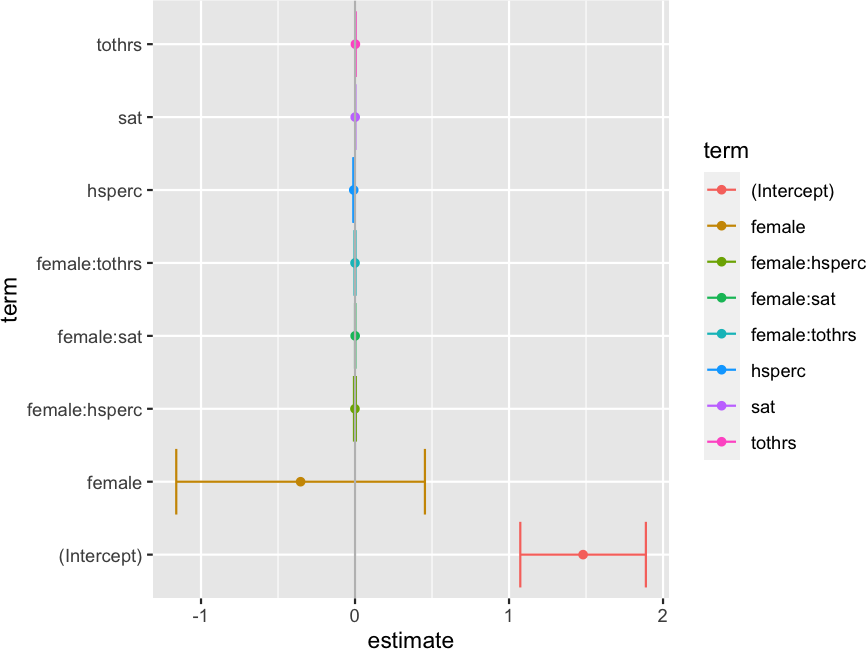
\includegraphics[width=0.8\linewidth]{MEM5220_R_files/figure-latex/fig17-1} 

}

\caption{Coefficient plots}\label{fig:fig17}
\end{figure}

To recap, the general form in which we specify regression models in R:

\begin{Shaded}
\begin{Highlighting}[]
\CommentTok{## response ~ terms}
\CommentTok{## }
\CommentTok{## y ~ age + sex            # age + sex main effects}
\CommentTok{## y ~ age + sex + age:sex  # add second-order interaction}
\CommentTok{## y ~ age*sex              # second-order interaction +}
\CommentTok{##                          # all main effects}
\CommentTok{## y ~ (age + sex + pressure)^2}
\CommentTok{##                          # age+sex+pressure+age:sex+age:pressure...}
\CommentTok{## y ~ (age + sex + pressure)^2 - sex:pressure}
\CommentTok{##                          # all main effects and all 2nd order}
\CommentTok{##                          # interactions except sex:pressure}
\CommentTok{## y ~ (age + race)*sex     # age+race+sex+age:sex+race:sex}
\CommentTok{## y ~ treatment*(age*race + age*sex) # no interact. with race,sex}
\CommentTok{## sqrt(y) ~ sex*sqrt(age) + race}
\CommentTok{## # functions, with dummy variables generated if}
\CommentTok{## # race is an R factor (classification) variable}
\CommentTok{## y ~ sex + poly(age,2)    # poly generates orthogonal polynomials}
\CommentTok{## race.sex <- interaction(race,sex)}
\CommentTok{## y ~ age + race.sex       # for when you want dummy variables for}
\CommentTok{##                          # all combinations of the factors}
\end{Highlighting}
\end{Shaded}

\hypertarget{heteroskedasticity}{%
\section{Heteroskedasticity}\label{heteroskedasticity}}

The homoskedasticity assumptions SLR.5 and MLR.5 require that the
variance of the error term is unrelated to the regressors, i.e.

\begin{equation}
Var(u|x_1, \dots , x_n) = \sigma^2  
\end{equation}

Unbiasedness and consistency do not depend on this assumption, but the
sampling distribution does. If homoskedasticity is violated, the
standard errors are invalid and all inferences from \(t\), \(F\), and
other tests based on them are unreliable.

There are various ways of dealing with heteroskedasticity in R. The
\textbf{car} package provides linear hypothesis. For high-dimensional
fixed effects the \textbf{lfe} package is a good alternative. It also
allows to specify clusters as part of the formula. A good balance
between functionality and ease of use is provided by the
\textbf{sandwich} package \citet{Zeileis2017}.

\hypertarget{spotting-heteroskedasticity-in-scatter-plots}{%
\subsection{Spotting Heteroskedasticity in Scatter
Plots}\label{spotting-heteroskedasticity-in-scatter-plots}}

\begin{Shaded}
\begin{Highlighting}[]
\KeywordTok{data}\NormalTok{(}\StringTok{"food"}\NormalTok{,}\DataTypeTok{package=}\StringTok{"PoEdata"}\NormalTok{)}
\NormalTok{mod1 <-}\StringTok{ }\KeywordTok{lm}\NormalTok{(food_exp}\OperatorTok{~}\NormalTok{income, }\DataTypeTok{data=}\NormalTok{food)}
\KeywordTok{plot}\NormalTok{(food}\OperatorTok{$}\NormalTok{income,food}\OperatorTok{$}\NormalTok{food_exp, }\DataTypeTok{type=}\StringTok{"p"}\NormalTok{,}
     \DataTypeTok{xlab=}\StringTok{"income"}\NormalTok{, }\DataTypeTok{ylab=}\StringTok{"food expenditure"}\NormalTok{)}
\KeywordTok{abline}\NormalTok{(mod1)}
\end{Highlighting}
\end{Shaded}

\begin{figure}

{\centering 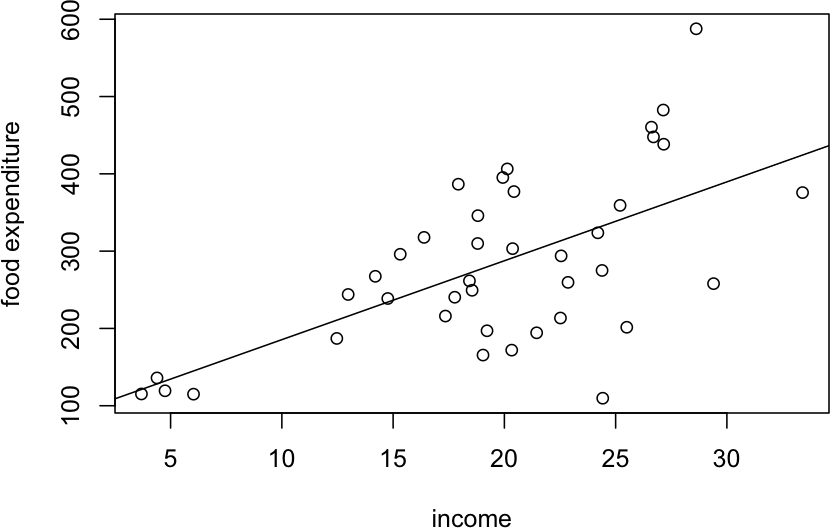
\includegraphics[width=0.8\linewidth]{MEM5220_R_files/figure-latex/fig18-1} 

}

\caption{Heteroskedasticity in the ‘food’ data}\label{fig:fig18}
\end{figure}

Another useful method to visualize possible heteroskedasticity is to
plot the residuals against the regressors suspected of creating
heteroskedasticity, or, more generally, against the fitted values of the
regression.

\begin{Shaded}
\begin{Highlighting}[]
\NormalTok{res <-}\StringTok{ }\KeywordTok{residuals}\NormalTok{(mod1)}
\NormalTok{yhat <-}\StringTok{ }\KeywordTok{fitted}\NormalTok{(mod1)}
\KeywordTok{plot}\NormalTok{(food}\OperatorTok{$}\NormalTok{income,res, }\DataTypeTok{xlab=}\StringTok{"income"}\NormalTok{, }\DataTypeTok{ylab=}\StringTok{"residuals"}\NormalTok{)}
\end{Highlighting}
\end{Shaded}

\begin{figure}

{\centering 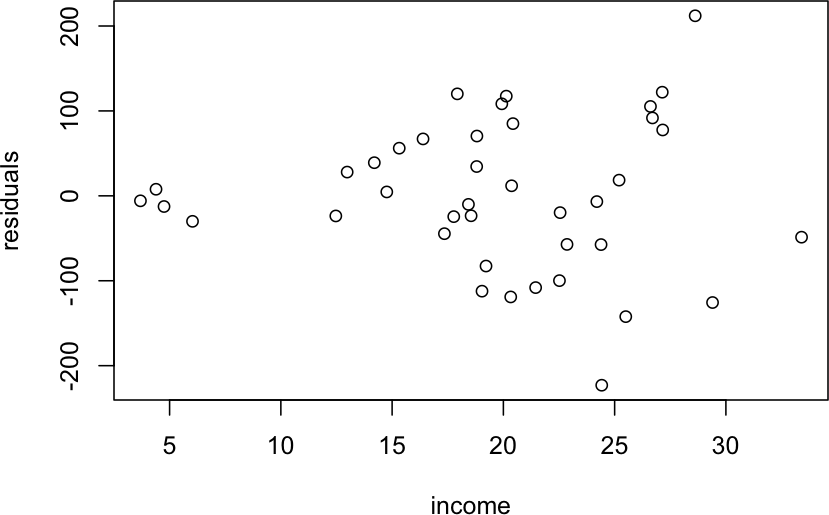
\includegraphics[width=0.8\linewidth]{MEM5220_R_files/figure-latex/fig19-1} 

}

\caption{Residual plots in the ‘food’ model }\label{fig:fig191}
\end{figure}

\begin{Shaded}
\begin{Highlighting}[]
\KeywordTok{plot}\NormalTok{(yhat,res, }\DataTypeTok{xlab=}\StringTok{"fitted values"}\NormalTok{, }\DataTypeTok{ylab=}\StringTok{"residuals"}\NormalTok{)}
\end{Highlighting}
\end{Shaded}

\begin{figure}

{\centering 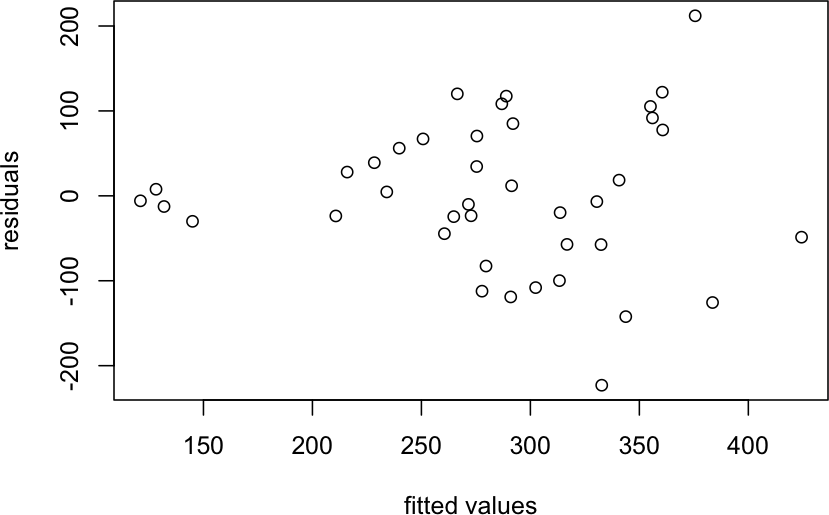
\includegraphics[width=0.8\linewidth]{MEM5220_R_files/figure-latex/fig19-2} 

}

\caption{Residual plots in the ‘food’ model }\label{fig:fig192}
\end{figure}

\hypertarget{heteroskedasticity-tests}{%
\subsection{Heteroskedasticity Tests}\label{heteroskedasticity-tests}}

\begin{Shaded}
\begin{Highlighting}[]
\KeywordTok{data}\NormalTok{(gpa3, }\DataTypeTok{package=}\StringTok{'wooldridge'}\NormalTok{)}


\CommentTok{# Estimate model (only for spring data)}
\NormalTok{reg <-}\StringTok{ }\KeywordTok{lm}\NormalTok{(cumgpa}\OperatorTok{~}\NormalTok{sat}\OperatorTok{+}\NormalTok{hsperc}\OperatorTok{+}\NormalTok{tothrs}\OperatorTok{+}\NormalTok{female}\OperatorTok{+}\NormalTok{black}\OperatorTok{+}\NormalTok{white, }
          \DataTypeTok{data=}\NormalTok{gpa3, }\DataTypeTok{subset=}\NormalTok{(spring}\OperatorTok{==}\DecValTok{1}\NormalTok{))}


\CommentTok{# Breusch-Pagan (BP) Test}

\KeywordTok{bptest}\NormalTok{(reg)}
\end{Highlighting}
\end{Shaded}

\begin{verbatim}
## 
##  studentized Breusch-Pagan test
## 
## data:  reg
## BP = 44.557, df = 6, p-value = 5.732e-08
\end{verbatim}

The R function that does this job is \texttt{hccm()}, which is part of
the car package and yields a heteroskedasticity-robust coefficient
covariance matrix. This matrix can then be used with other functions,
such as \texttt{coeftest()} (instead of summary), \texttt{waldtest()}
(instead of anova), or \texttt{linearHypothesis()} to perform hypothesis
testing. The function \texttt{hccm()} takes several arguments, among
which is the model for which we want the robust standard errors and the
type of standard errors we wish to calculate.

\begin{Shaded}
\begin{Highlighting}[]
\CommentTok{# Usual SE:}
\KeywordTok{coeftest}\NormalTok{(reg)}
\end{Highlighting}
\end{Shaded}

\begin{verbatim}
## 
## t test of coefficients:
## 
##                Estimate  Std. Error t value  Pr(>|t|)    
## (Intercept)  1.47006477  0.22980308  6.3971 4.942e-10 ***
## sat          0.00114073  0.00017856  6.3885 5.197e-10 ***
## hsperc      -0.00856636  0.00124042 -6.9060 2.275e-11 ***
## tothrs       0.00250400  0.00073099  3.4255 0.0006847 ***
## female       0.30343329  0.05902033  5.1412 4.497e-07 ***
## black       -0.12828368  0.14737012 -0.8705 0.3846164    
## white       -0.05872173  0.14098956 -0.4165 0.6772953    
## ---
## Signif. codes:  0 '***' 0.001 '**' 0.01 '*' 0.05 '.' 0.1 ' ' 1
\end{verbatim}

\begin{Shaded}
\begin{Highlighting}[]
\CommentTok{# Refined White heteroscedasticity-robust SE:}
\KeywordTok{coeftest}\NormalTok{(reg, }\DataTypeTok{vcov=}\NormalTok{hccm)}
\end{Highlighting}
\end{Shaded}

\begin{verbatim}
## 
## t test of coefficients:
## 
##                Estimate  Std. Error t value  Pr(>|t|)    
## (Intercept)  1.47006477  0.22938036  6.4089 4.611e-10 ***
## sat          0.00114073  0.00019532  5.8402 1.169e-08 ***
## hsperc      -0.00856636  0.00144359 -5.9341 6.963e-09 ***
## tothrs       0.00250400  0.00074930  3.3418   0.00092 ***
## female       0.30343329  0.06003964  5.0539 6.911e-07 ***
## black       -0.12828368  0.12818828 -1.0007   0.31762    
## white       -0.05872173  0.12043522 -0.4876   0.62615    
## ---
## Signif. codes:  0 '***' 0.001 '**' 0.01 '*' 0.05 '.' 0.1 ' ' 1
\end{verbatim}

\begin{Shaded}
\begin{Highlighting}[]
\NormalTok{cov3 <-}\StringTok{ }\KeywordTok{hccm}\NormalTok{(reg, }\DataTypeTok{type=}\StringTok{"hc3"}\NormalTok{) }\CommentTok{# hc3 is the standard method}
\NormalTok{ref.HC3 <-}\StringTok{ }\KeywordTok{coeftest}\NormalTok{(reg, }\DataTypeTok{vcov.=}\NormalTok{cov3)}

\CommentTok{# Supply other White corrections}
\NormalTok{cov1 <-}\StringTok{ }\KeywordTok{hccm}\NormalTok{(reg, }\DataTypeTok{type=}\StringTok{"hc1"}\NormalTok{)}
\NormalTok{ref.HC1 <-}\StringTok{ }\KeywordTok{coeftest}\NormalTok{(reg, }\DataTypeTok{vcov.=}\NormalTok{cov1)}
\end{Highlighting}
\end{Shaded}

Another way of dealing with heteroskedasticity is to use the
\texttt{lmrob()} function from the \textbf{robustbase} package\footnote{This
  example has been adapted from the blog post of \citet{Rodrigues2018}}.
This package is quite interesting, and offers quite a lot of functions
for robust linear, and nonlinear, regression models. Running a robust
linear regression is just the same as with \texttt{lm()}:

\begin{Shaded}
\begin{Highlighting}[]
\NormalTok{regrobfit <-}\StringTok{ }\KeywordTok{lmrob}\NormalTok{(cumgpa}\OperatorTok{~}\NormalTok{sat}\OperatorTok{+}\NormalTok{hsperc}\OperatorTok{+}\NormalTok{tothrs}\OperatorTok{+}\NormalTok{female}\OperatorTok{+}\NormalTok{black}\OperatorTok{+}\NormalTok{white, }
                   \DataTypeTok{data=}\NormalTok{gpa3, }\DataTypeTok{subset=}\NormalTok{(spring}\OperatorTok{==}\DecValTok{1}\NormalTok{))}

\KeywordTok{summary}\NormalTok{(regrobfit)}
\end{Highlighting}
\end{Shaded}

\begin{verbatim}
## 
## Call:
## lmrob(formula = cumgpa ~ sat + hsperc + tothrs + female + black + white, 
##     data = gpa3, subset = (spring == 1))
##  \--> method = "MM"
## Residuals:
##      Min       1Q   Median       3Q      Max 
## -1.57535 -0.30124 -0.02834  0.26687  1.27950 
## 
## Coefficients:
##               Estimate Std. Error t value Pr(>|t|)    
## (Intercept)  1.4693758  0.2315018   6.347 6.62e-10 ***
## sat          0.0011185  0.0001953   5.727 2.17e-08 ***
## hsperc      -0.0079056  0.0014293  -5.531 6.14e-08 ***
## tothrs       0.0021841  0.0007750   2.818   0.0051 ** 
## female       0.3002542  0.0599150   5.011 8.50e-07 ***
## black       -0.1281927  0.1268974  -1.010   0.3131    
## white       -0.0305168  0.1181863  -0.258   0.7964    
## ---
## Signif. codes:  0 '***' 0.001 '**' 0.01 '*' 0.05 '.' 0.1 ' ' 1
## 
## Robust residual standard error: 0.4201 
## Multiple R-squared:  0.411,  Adjusted R-squared:  0.4012 
## Convergence in 15 IRWLS iterations
## 
## Robustness weights: 
##  22 weights are ~= 1. The remaining 344 ones are summarized as
##    Min. 1st Qu.  Median    Mean 3rd Qu.    Max. 
##  0.1291  0.8670  0.9471  0.8933  0.9854  0.9987 
## Algorithmic parameters: 
##        tuning.chi                bb        tuning.psi        refine.tol 
##         1.548e+00         5.000e-01         4.685e+00         1.000e-07 
##           rel.tol         scale.tol         solve.tol       eps.outlier 
##         1.000e-07         1.000e-10         1.000e-07         2.732e-04 
##             eps.x warn.limit.reject warn.limit.meanrw 
##         2.601e-09         5.000e-01         5.000e-01 
##      nResample         max.it       best.r.s       k.fast.s          k.max 
##            500             50              2              1            200 
##    maxit.scale      trace.lev            mts     compute.rd fast.s.large.n 
##            200              0           1000              0           2000 
##                   psi           subsampling                   cov 
##            "bisquare"         "nonsingular"         ".vcov.avar1" 
## compute.outlier.stats 
##                  "SM" 
## seed : int(0)
\end{verbatim}

This however, gives you different estimates than when fitting a linear
regression model. The estimates should be the same, only the standard
errors should be different. This is because the estimation method is
different, and is also robust to outlines (at least that's my
understanding, I haven't read the theoretical papers behind the package
yet).

Finally, it is also possible to bootstrap the standard errors. For this
I will use the \texttt{bootstrap()} function from the modelr package:

\begin{Shaded}
\begin{Highlighting}[]
\NormalTok{resamples <-}\StringTok{ }\DecValTok{100}

\NormalTok{boot_gpa3 <-}\StringTok{ }\NormalTok{gpa3 }\OperatorTok\StringTok{ }
\StringTok{  }\NormalTok{modelr}\OperatorTok{::}\KeywordTok{bootstrap}\NormalTok{(resamples)}
\end{Highlighting}
\end{Shaded}

The column strap contains resamples of the original data. I will run my
linear regression from before on each of the resamples:

\begin{Shaded}
\begin{Highlighting}[]
\NormalTok{boot_lin_reg <-}\StringTok{ }\NormalTok{boot_gpa3 }\OperatorTok\StringTok{ }
\StringTok{  }\KeywordTok{mutate}\NormalTok{(}\DataTypeTok{regressions =} 
           \KeywordTok{map}\NormalTok{(strap, }
               \OperatorTok{~}\KeywordTok{lm}\NormalTok{(cumgpa}\OperatorTok{~}\NormalTok{sat}\OperatorTok{+}\NormalTok{hsperc}\OperatorTok{+}\NormalTok{tothrs}\OperatorTok{+}\NormalTok{female}\OperatorTok{+}\NormalTok{black}\OperatorTok{+}\NormalTok{white, }
                   \DataTypeTok{data=}\NormalTok{ . , }\DataTypeTok{subset=}\NormalTok{(spring}\OperatorTok{==}\DecValTok{1}\NormalTok{)))}
\NormalTok{  )}
\end{Highlighting}
\end{Shaded}

We have added a new column called regressions which contains the linear
regressions on each bootstrapped sample. Now, I will create a list of
tidied regression results:

\begin{Shaded}
\begin{Highlighting}[]
\NormalTok{tidied <-}\StringTok{ }\NormalTok{boot_lin_reg }\OperatorTok\StringTok{ }
\StringTok{  }\KeywordTok{mutate}\NormalTok{(}\DataTypeTok{tidy_lm =} 
           \KeywordTok{map}\NormalTok{(regressions, broom}\OperatorTok{::}\NormalTok{tidy))}
\end{Highlighting}
\end{Shaded}

\begin{Shaded}
\begin{Highlighting}[]
\NormalTok{tidied}\OperatorTok{$}\NormalTok{tidy_lm[[}\DecValTok{1}\NormalTok{]]}
\end{Highlighting}
\end{Shaded}

\textbackslash{}begin\{table\}{[}h{]}
\textbackslash{}begin\{raggedright\}

\providecommand{\huxb}[2][0,0,0]{\arrayrulecolor[RGB]{#1}\global\arrayrulewidth=#2pt}
    \providecommand{\huxvb}[2][0,0,0]{\color[RGB]{#1}\vrule width #2pt}
    \providecommand{\huxtpad}[1]{\rule{0pt}{\baselineskip+#1}}
    \providecommand{\huxbpad}[1]{\rule[-#1]{0pt}{#1}}
  \begin{tabularx}{0.988888888888889\textwidth}{p{0.197777777777778\textwidth} p{0.197777777777778\textwidth} p{0.197777777777778\textwidth} p{0.197777777777778\textwidth} p{0.197777777777778\textwidth}}


\par

\textbackslash{}end\{raggedright\} \textbackslash{}end\{table\}

\begin{Shaded}
\begin{Highlighting}[]
\NormalTok{list_mods <-}\StringTok{ }\NormalTok{tidied }\OperatorTok\StringTok{ }
\StringTok{  }\KeywordTok{pull}\NormalTok{(tidy_lm)}
\end{Highlighting}
\end{Shaded}

\begin{Shaded}
\begin{Highlighting}[]
\NormalTok{mods_df <-}\StringTok{ }\KeywordTok{map2_df}\NormalTok{(list_mods, }
                   \KeywordTok{seq}\NormalTok{(}\DecValTok{1}\NormalTok{, resamples), }
                   \OperatorTok{~}\KeywordTok{mutate}\NormalTok{(.x, }\DataTypeTok{resample =}\NormalTok{ .y))}
\end{Highlighting}
\end{Shaded}

\begin{Shaded}
\begin{Highlighting}[]
\KeywordTok{head}\NormalTok{(mods_df, }\DecValTok{5}\NormalTok{)}
\end{Highlighting}
\end{Shaded}

\textbackslash{}begin\{table\}{[}h{]}
\textbackslash{}begin\{raggedright\}

\providecommand{\huxb}[2][0,0,0]{\arrayrulecolor[RGB]{#1}\global\arrayrulewidth=#2pt}
    \providecommand{\huxvb}[2][0,0,0]{\color[RGB]{#1}\vrule width #2pt}
    \providecommand{\huxtpad}[1]{\rule{0pt}{\baselineskip+#1}}
    \providecommand{\huxbpad}[1]{\rule[-#1]{0pt}{#1}}
  \begin{tabularx}{0.977777777777778\textwidth}{p{0.162962962962963\textwidth} p{0.162962962962963\textwidth} p{0.162962962962963\textwidth} p{0.162962962962963\textwidth} p{0.162962962962963\textwidth} p{0.162962962962963\textwidth}}


\par

\textbackslash{}end\{raggedright\} \textbackslash{}end\{table\}

\begin{Shaded}
\begin{Highlighting}[]
\NormalTok{r.std.error <-}\StringTok{ }\NormalTok{mods_df }\OperatorTok\StringTok{ }
\StringTok{  }\KeywordTok{group_by}\NormalTok{(term) }\OperatorTok\StringTok{ }
\StringTok{  }\KeywordTok{summarise}\NormalTok{(}\DataTypeTok{r.std.error =} \KeywordTok{sd}\NormalTok{(estimate))}
\end{Highlighting}
\end{Shaded}

\begin{Shaded}
\begin{Highlighting}[]
\NormalTok{reg }\OperatorTok\StringTok{ }
\StringTok{  }\NormalTok{broom}\OperatorTok{::}\KeywordTok{tidy}\NormalTok{()   }\OperatorTok\StringTok{ }
\StringTok{  }\KeywordTok{full_join}\NormalTok{(r.std.error)}
\end{Highlighting}
\end{Shaded}

\begin{verbatim}
## Joining, by = "term"
\end{verbatim}

\textbackslash{}begin\{table\}{[}h{]}
\textbackslash{}begin\{raggedright\}

\providecommand{\huxb}[2][0,0,0]{\arrayrulecolor[RGB]{#1}\global\arrayrulewidth=#2pt}
    \providecommand{\huxvb}[2][0,0,0]{\color[RGB]{#1}\vrule width #2pt}
    \providecommand{\huxtpad}[1]{\rule{0pt}{\baselineskip+#1}}
    \providecommand{\huxbpad}[1]{\rule[-#1]{0pt}{#1}}
  \begin{tabularx}{1\textwidth}{p{0.166666666666667\textwidth} p{0.166666666666667\textwidth} p{0.166666666666667\textwidth} p{0.166666666666667\textwidth} p{0.166666666666667\textwidth} p{0.166666666666667\textwidth}}


\par

\textbackslash{}end\{raggedright\} \textbackslash{}end\{table\}

Using the whole bootstrapping procedure is longer than simply using
either one of the first two methods. However, this procedure is very
flexible and can thus be adapted to a very large range of situations.

\hypertarget{weighted-least-squares}{%
\section{Weighted least squares}\label{weighted-least-squares}}

Weighted Least Squares (WLS) attempts to provide a more efficient
alternative to OLS. It is a special version of a feasible generalized
least squares (FGLS) estimator.

\begin{Shaded}
\begin{Highlighting}[]
\KeywordTok{data}\NormalTok{(}\StringTok{"k401k"}\NormalTok{)}
\end{Highlighting}
\end{Shaded}

\begin{Shaded}
\begin{Highlighting}[]
\CommentTok{# OLS (only for singles: fsize==1)}
\KeywordTok{lm}\NormalTok{(nettfa }\OperatorTok{~}\StringTok{ }\NormalTok{inc }\OperatorTok{+}\StringTok{ }\KeywordTok{I}\NormalTok{((age}\DecValTok{-25}\NormalTok{)}\OperatorTok{^}\DecValTok{2}\NormalTok{) }\OperatorTok{+}\StringTok{ }\NormalTok{male }\OperatorTok{+}\StringTok{ }\NormalTok{e401k, }
   \DataTypeTok{data=}\NormalTok{k401ksubs, }\DataTypeTok{subset=}\NormalTok{(fsize}\OperatorTok{==}\DecValTok{1}\NormalTok{))}
\end{Highlighting}
\end{Shaded}

\begin{verbatim}
## 
## Call:
## lm(formula = nettfa ~ inc + I((age - 25)^2) + male + e401k, data = k401ksubs, 
##     subset = (fsize == 1))
## 
## Coefficients:
##     (Intercept)              inc  I((age - 25)^2)             male  
##       -20.98499          0.77058          0.02513          2.47793  
##           e401k  
##         6.88622
\end{verbatim}

Following Wooldrige, we assume that the variance is proportional to the
income variable \emph{inc.}. Therefore, the optimal weight is
\(\frac{1}{inc}\) which is given as \emph{weight} in the \texttt{lm()}
call.

\begin{Shaded}
\begin{Highlighting}[]
\CommentTok{# WLS}
\KeywordTok{lm}\NormalTok{(nettfa }\OperatorTok{~}\StringTok{ }\NormalTok{inc }\OperatorTok{+}\StringTok{ }\KeywordTok{I}\NormalTok{((age}\DecValTok{-25}\NormalTok{)}\OperatorTok{^}\DecValTok{2}\NormalTok{) }\OperatorTok{+}\StringTok{ }\NormalTok{male }\OperatorTok{+}\StringTok{ }\NormalTok{e401k, }\DataTypeTok{weight=}\DecValTok{1}\OperatorTok{/}\NormalTok{inc, }
   \DataTypeTok{data=}\NormalTok{k401ksubs, }\DataTypeTok{subset=}\NormalTok{(fsize}\OperatorTok{==}\DecValTok{1}\NormalTok{))}
\end{Highlighting}
\end{Shaded}

\begin{verbatim}
## 
## Call:
## lm(formula = nettfa ~ inc + I((age - 25)^2) + male + e401k, data = k401ksubs, 
##     subset = (fsize == 1), weights = 1/inc)
## 
## Coefficients:
##     (Intercept)              inc  I((age - 25)^2)             male  
##       -16.70252          0.74038          0.01754          1.84053  
##           e401k  
##         5.18828
\end{verbatim}

We can also use heteroscedasticity-robust statistics to account for the
fact that our variance function might be misspecified.

\begin{Shaded}
\begin{Highlighting}[]
\CommentTok{# WLS}
\NormalTok{wlsreg <-}\StringTok{ }\KeywordTok{lm}\NormalTok{(nettfa }\OperatorTok{~}\StringTok{ }\NormalTok{inc }\OperatorTok{+}\StringTok{ }\KeywordTok{I}\NormalTok{((age}\DecValTok{-25}\NormalTok{)}\OperatorTok{^}\DecValTok{2}\NormalTok{) }\OperatorTok{+}\StringTok{ }\NormalTok{male }\OperatorTok{+}\StringTok{ }\NormalTok{e401k, }
             \DataTypeTok{weight=}\DecValTok{1}\OperatorTok{/}\NormalTok{inc, }\DataTypeTok{data=}\NormalTok{k401ksubs, }\DataTypeTok{subset=}\NormalTok{(fsize}\OperatorTok{==}\DecValTok{1}\NormalTok{))}

\CommentTok{# non-robust results}
\KeywordTok{coeftest}\NormalTok{(wlsreg)}
\end{Highlighting}
\end{Shaded}

\begin{verbatim}
## 
## t test of coefficients:
## 
##                    Estimate  Std. Error t value  Pr(>|t|)    
## (Intercept)     -16.7025205   1.9579947 -8.5304 < 2.2e-16 ***
## inc               0.7403843   0.0643029 11.5140 < 2.2e-16 ***
## I((age - 25)^2)   0.0175373   0.0019315  9.0796 < 2.2e-16 ***
## male              1.8405293   1.5635872  1.1771  0.239287    
## e401k             5.1882807   1.7034258  3.0458  0.002351 ** 
## ---
## Signif. codes:  0 '***' 0.001 '**' 0.01 '*' 0.05 '.' 0.1 ' ' 1
\end{verbatim}

\begin{Shaded}
\begin{Highlighting}[]
\CommentTok{# robust results (Refined White SE:)}
\KeywordTok{coeftest}\NormalTok{(wlsreg,hccm)}
\end{Highlighting}
\end{Shaded}

\begin{verbatim}
## 
## t test of coefficients:
## 
##                    Estimate  Std. Error t value  Pr(>|t|)    
## (Intercept)     -16.7025205   2.2482355 -7.4292 1.606e-13 ***
## inc               0.7403843   0.0752396  9.8403 < 2.2e-16 ***
## I((age - 25)^2)   0.0175373   0.0025924  6.7650 1.742e-11 ***
## male              1.8405293   1.3132477  1.4015 0.1612159    
## e401k             5.1882807   1.5743329  3.2955 0.0009994 ***
## ---
## Signif. codes:  0 '***' 0.001 '**' 0.01 '*' 0.05 '.' 0.1 ' ' 1
\end{verbatim}

\begin{Shaded}
\begin{Highlighting}[]
\KeywordTok{coeftest}\NormalTok{(wlsreg, }\DataTypeTok{vcov. =}\NormalTok{ vcovHC)}
\end{Highlighting}
\end{Shaded}

\begin{verbatim}
## 
## t test of coefficients:
## 
##                    Estimate  Std. Error t value  Pr(>|t|)    
## (Intercept)     -16.7025205   2.2482355 -7.4292 1.606e-13 ***
## inc               0.7403843   0.0752396  9.8403 < 2.2e-16 ***
## I((age - 25)^2)   0.0175373   0.0025924  6.7650 1.742e-11 ***
## male              1.8405293   1.3132477  1.4015 0.1612159    
## e401k             5.1882807   1.5743329  3.2955 0.0009994 ***
## ---
## Signif. codes:  0 '***' 0.001 '**' 0.01 '*' 0.05 '.' 0.1 ' ' 1
\end{verbatim}

\begin{Shaded}
\begin{Highlighting}[]
\NormalTok{mySummary <-}\StringTok{ }\ControlFlowTok{function}\NormalTok{(model, VCOV) \{}
  \KeywordTok{print}\NormalTok{(}\KeywordTok{coeftest}\NormalTok{(model, }\DataTypeTok{vcov. =}\NormalTok{ VCOV))}
  \KeywordTok{print}\NormalTok{(}\KeywordTok{waldtest}\NormalTok{(model, }\DataTypeTok{vcov =}\NormalTok{ VCOV))}
\NormalTok{\}}
\KeywordTok{mySummary}\NormalTok{(wlsreg, }\DataTypeTok{VCOV =}\NormalTok{ vcovHAC)}
\end{Highlighting}
\end{Shaded}

\begin{verbatim}
## 
## t test of coefficients:
## 
##                    Estimate  Std. Error t value  Pr(>|t|)    
## (Intercept)     -16.7025205   2.2425229 -7.4481 1.397e-13 ***
## inc               0.7403843   0.0752621  9.8374 < 2.2e-16 ***
## I((age - 25)^2)   0.0175373   0.0025797  6.7981 1.392e-11 ***
## male              1.8405293   1.3056244  1.4097  0.158785    
## e401k             5.1882807   1.5733280  3.2976  0.000992 ***
## ---
## Signif. codes:  0 '***' 0.001 '**' 0.01 '*' 0.05 '.' 0.1 ' ' 1
## 
## Wald test
## 
## Model 1: nettfa ~ inc + I((age - 25)^2) + male + e401k
## Model 2: nettfa ~ 1
##   Res.Df Df      F    Pr(>F)    
## 1   2012                        
## 2   2016 -4 39.602 < 2.2e-16 ***
## ---
## Signif. codes:  0 '***' 0.001 '**' 0.01 '*' 0.05 '.' 0.1 ' ' 1
\end{verbatim}

The assumption that the variance is proportional to a regressor is
usually hard to justify. Typically, we do not know the variance
function; we have to estimate it. We can estimate the relation between
variance and regressors using a linear regression of the log of the
squared residuals from an initial OLS regression \(log(\hat{u}^{2})\) as
the dependent variable.

Wooldrige suggests two version for the selection of regressors:

\begin{itemize}
\tightlist
\item
  the regressors \(x_1, \dots , x_k\) from the original model similar to
  the BP test
\item
  \(\hat{y}\) and \(\hat{y}^{2}\) from the original model similar to the
  White test
\end{itemize}

\begin{Shaded}
\begin{Highlighting}[]
\KeywordTok{data}\NormalTok{(}\StringTok{"smoke"}\NormalTok{)}
\CommentTok{# OLS}
\NormalTok{olsreg<-}\KeywordTok{lm}\NormalTok{(cigs}\OperatorTok{~}\KeywordTok{log}\NormalTok{(income)}\OperatorTok{+}\KeywordTok{log}\NormalTok{(cigpric)}\OperatorTok{+}\NormalTok{educ}\OperatorTok{+}\NormalTok{age}\OperatorTok{+}\KeywordTok{I}\NormalTok{(age}\OperatorTok{^}\DecValTok{2}\NormalTok{)}\OperatorTok{+}\NormalTok{restaurn, }
           \DataTypeTok{data=}\NormalTok{smoke)}
\NormalTok{olsreg}
\end{Highlighting}
\end{Shaded}

\begin{verbatim}
## 
## Call:
## lm(formula = cigs ~ log(income) + log(cigpric) + educ + age + 
##     I(age^2) + restaurn, data = smoke)
## 
## Coefficients:
##  (Intercept)   log(income)  log(cigpric)          educ           age  
##    -3.639826      0.880268     -0.750862     -0.501498      0.770694  
##     I(age^2)      restaurn  
##    -0.009023     -2.825085
\end{verbatim}

\begin{Shaded}
\begin{Highlighting}[]
\CommentTok{# BP test}
\KeywordTok{bptest}\NormalTok{(olsreg)}
\end{Highlighting}
\end{Shaded}

\begin{verbatim}
## 
##  studentized Breusch-Pagan test
## 
## data:  olsreg
## BP = 32.258, df = 6, p-value = 1.456e-05
\end{verbatim}

\begin{Shaded}
\begin{Highlighting}[]
\CommentTok{# FGLS: estimation of the variance function}
\NormalTok{logu2 <-}\StringTok{ }\KeywordTok{log}\NormalTok{(}\KeywordTok{resid}\NormalTok{(olsreg)}\OperatorTok{^}\DecValTok{2}\NormalTok{)}
\NormalTok{varreg<-}\KeywordTok{lm}\NormalTok{(logu2}\OperatorTok{~}\KeywordTok{log}\NormalTok{(income)}\OperatorTok{+}\KeywordTok{log}\NormalTok{(cigpric)}\OperatorTok{+}\NormalTok{educ}\OperatorTok{+}\NormalTok{age}\OperatorTok{+}\KeywordTok{I}\NormalTok{(age}\OperatorTok{^}\DecValTok{2}\NormalTok{)}\OperatorTok{+}\NormalTok{restaurn, }
           \DataTypeTok{data=}\NormalTok{smoke)}

\CommentTok{# FGLS: WLS}
\NormalTok{w <-}\StringTok{ }\DecValTok{1}\OperatorTok{/}\KeywordTok{exp}\NormalTok{(}\KeywordTok{fitted}\NormalTok{(varreg))}
\KeywordTok{lm}\NormalTok{(cigs}\OperatorTok{~}\KeywordTok{log}\NormalTok{(income)}\OperatorTok{+}\KeywordTok{log}\NormalTok{(cigpric)}\OperatorTok{+}\NormalTok{educ}\OperatorTok{+}\NormalTok{age}\OperatorTok{+}\KeywordTok{I}\NormalTok{(age}\OperatorTok{^}\DecValTok{2}\NormalTok{)}\OperatorTok{+}\NormalTok{restaurn, }
   \DataTypeTok{weight=}\NormalTok{w ,}\DataTypeTok{data=}\NormalTok{smoke)}
\end{Highlighting}
\end{Shaded}

\begin{verbatim}
## 
## Call:
## lm(formula = cigs ~ log(income) + log(cigpric) + educ + age + 
##     I(age^2) + restaurn, data = smoke, weights = w)
## 
## Coefficients:
##  (Intercept)   log(income)  log(cigpric)          educ           age  
##     5.635463      1.295239     -2.940312     -0.463446      0.481948  
##     I(age^2)      restaurn  
##    -0.005627     -3.461064
\end{verbatim}

\hypertarget{model-specification-and-parameter-heterogeneity}{%
\section{Model specification and Parameter
Heterogeneity}\label{model-specification-and-parameter-heterogeneity}}

\hypertarget{functional-form-misspecifcation}{%
\subsection{Functional Form
Misspecifcation}\label{functional-form-misspecifcation}}

We have seen many ways to specify the relation between the dependent
variable and the regressors. An obvious question is to ask whether or
not a given specification is ``correct''.

\hypertarget{reset}{%
\subsubsection{RESET}\label{reset}}

The Regression Equation Specification Error Test (RESET) is a convenient
tool to test the null hypothesis that the functional form is adequate.

We can run the test ourselves or use the boxed routine
\texttt{resettest()} from the package \textbf{lmtest}.

\begin{Shaded}
\begin{Highlighting}[]
\KeywordTok{data}\NormalTok{(}\StringTok{"hprice1"}\NormalTok{)}
\CommentTok{# original linear regression}
\NormalTok{orig <-}\StringTok{ }\KeywordTok{lm}\NormalTok{(price }\OperatorTok{~}\StringTok{ }\NormalTok{lotsize}\OperatorTok{+}\NormalTok{sqrft}\OperatorTok{+}\NormalTok{bdrms, }\DataTypeTok{data=}\NormalTok{hprice1)}

\CommentTok{# regression for RESET test}
\NormalTok{RESETreg <-}\StringTok{ }\KeywordTok{lm}\NormalTok{(price }\OperatorTok{~}\StringTok{ }\NormalTok{lotsize}\OperatorTok{+}\NormalTok{sqrft}\OperatorTok{+}\NormalTok{bdrms}\OperatorTok{+}\KeywordTok{I}\NormalTok{(}\KeywordTok{fitted}\NormalTok{(orig)}\OperatorTok{^}\DecValTok{2}\NormalTok{)}\OperatorTok{+}\StringTok{ }
\StringTok{                 }\KeywordTok{I}\NormalTok{(}\KeywordTok{fitted}\NormalTok{(orig)}\OperatorTok{^}\DecValTok{3}\NormalTok{), }\DataTypeTok{data=}\NormalTok{hprice1)}
\NormalTok{RESETreg}
\end{Highlighting}
\end{Shaded}

\begin{verbatim}
## 
## Call:
## lm(formula = price ~ lotsize + sqrft + bdrms + I(fitted(orig)^2) + 
##     I(fitted(orig)^3), data = hprice1)
## 
## Coefficients:
##       (Intercept)            lotsize              sqrft  
##         1.661e+02          1.537e-04          1.760e-02  
##             bdrms  I(fitted(orig)^2)  I(fitted(orig)^3)  
##         2.175e+00          3.534e-04          1.546e-06
\end{verbatim}

\begin{Shaded}
\begin{Highlighting}[]
\CommentTok{# RESET test. H0: all coeffs including "fitted" are=0 }
\KeywordTok{linearHypothesis}\NormalTok{(RESETreg, }\KeywordTok{matchCoefs}\NormalTok{(RESETreg,}\StringTok{"fitted"}\NormalTok{))}
\end{Highlighting}
\end{Shaded}

\textbackslash{}begin\{table\}{[}h{]}
\textbackslash{}begin\{raggedright\}

\providecommand{\huxb}[2][0,0,0]{\arrayrulecolor[RGB]{#1}\global\arrayrulewidth=#2pt}
    \providecommand{\huxvb}[2][0,0,0]{\color[RGB]{#1}\vrule width #2pt}
    \providecommand{\huxtpad}[1]{\rule{0pt}{\baselineskip+#1}}
    \providecommand{\huxbpad}[1]{\rule[-#1]{0pt}{#1}}
  \begin{tabularx}{0.766666666666667\textwidth}{p{0.127777777777778\textwidth} p{0.127777777777778\textwidth} p{0.127777777777778\textwidth} p{0.127777777777778\textwidth} p{0.127777777777778\textwidth} p{0.127777777777778\textwidth}}


\par

\textbackslash{}end\{raggedright\} \textbackslash{}end\{table\}

Automatic routine:

\begin{Shaded}
\begin{Highlighting}[]
\CommentTok{# original linear regression}
\NormalTok{orig <-}\StringTok{ }\KeywordTok{lm}\NormalTok{(price }\OperatorTok{~}\StringTok{ }\NormalTok{lotsize}\OperatorTok{+}\NormalTok{sqrft}\OperatorTok{+}\NormalTok{bdrms, }\DataTypeTok{data=}\NormalTok{hprice1)}

\CommentTok{# RESET test}
\KeywordTok{resettest}\NormalTok{(orig)}
\end{Highlighting}
\end{Shaded}

\begin{verbatim}
## 
##  RESET test
## 
## data:  orig
## RESET = 4.6682, df1 = 2, df2 = 82, p-value = 0.01202
\end{verbatim}

Wooldrige (2016, Section 9.2) also discusses tests of non-nested models.
We can use the \texttt{encomptest()} function from the package
\textbf{lmtest}.

Two alternative models for the housing price

\begin{equation}
price = \beta_0 + \beta_1 lotsize  +\beta_2 sqrft  +\beta_3 bdrms  + u 
\end{equation}

\begin{equation}
price = \beta_0 + \beta_1 log(lotsize)  +\beta_2 log(sqrft)  +\beta_3 log(bdrms)  + u 
\end{equation}

\begin{Shaded}
\begin{Highlighting}[]
\CommentTok{# two alternative models}
\NormalTok{model1 <-}\StringTok{ }\KeywordTok{lm}\NormalTok{(price }\OperatorTok{~}\StringTok{     }\NormalTok{lotsize  }\OperatorTok{+}\StringTok{     }\NormalTok{sqrft  }\OperatorTok{+}\StringTok{ }\NormalTok{bdrms, }\DataTypeTok{data=}\NormalTok{hprice1)}
\NormalTok{model2 <-}\StringTok{ }\KeywordTok{lm}\NormalTok{(price }\OperatorTok{~}\StringTok{ }\KeywordTok{log}\NormalTok{(lotsize) }\OperatorTok{+}\StringTok{ }\KeywordTok{log}\NormalTok{(sqrft) }\OperatorTok{+}\StringTok{ }\NormalTok{bdrms, }\DataTypeTok{data=}\NormalTok{hprice1)}

\CommentTok{# Test against comprehensive model}
\KeywordTok{encomptest}\NormalTok{(model1,model2, }\DataTypeTok{data=}\NormalTok{hprice1)}
\end{Highlighting}
\end{Shaded}

\textbackslash{}begin\{table\}{[}h{]}
\textbackslash{}begin\{raggedright\}

\providecommand{\huxb}[2][0,0,0]{\arrayrulecolor[RGB]{#1}\global\arrayrulewidth=#2pt}
    \providecommand{\huxvb}[2][0,0,0]{\color[RGB]{#1}\vrule width #2pt}
    \providecommand{\huxtpad}[1]{\rule{0pt}{\baselineskip+#1}}
    \providecommand{\huxbpad}[1]{\rule[-#1]{0pt}{#1}}
  \begin{tabularx}{0.444444444444444\textwidth}{p{0.111111111111111\textwidth} p{0.111111111111111\textwidth} p{0.111111111111111\textwidth} p{0.111111111111111\textwidth}}


\par

\textbackslash{}end\{raggedright\} \textbackslash{}end\{table\}

The output shows the ``encompassing model'' \(E\) with all variables.
Both models are rejected against this comprehensive model.

\hypertarget{outlying-observations}{%
\subsubsection{Outlying observations}\label{outlying-observations}}

Dealing with outliers is a tricky business. R offers different packages
to test and adjust for outliers. But outliers can be a matter of opinion
and not all outlier detection methods give the same results. With the
\textbf{OutliersO3} package we can compare different outlier detection
methods.

\begin{Shaded}
\begin{Highlighting}[]
\KeywordTok{data}\NormalTok{(rdchem)}
\NormalTok{s3 <-}\StringTok{ }\KeywordTok{O3prep}\NormalTok{(rdchem, }\DataTypeTok{method=}\KeywordTok{c}\NormalTok{(}\StringTok{"HDo"}\NormalTok{, }\StringTok{"adjOut"}\NormalTok{, }\StringTok{"DDC"}\NormalTok{))}
\NormalTok{O3s3 <-}\StringTok{ }\KeywordTok{O3plotM}\NormalTok{(s3)}
\KeywordTok{print}\NormalTok{(O3s3}\OperatorTok{$}\NormalTok{nOut)}
\end{Highlighting}
\end{Shaded}

\begin{verbatim}
##    HDo adjOut    DDC 
##     10      1     11
\end{verbatim}

\begin{Shaded}
\begin{Highlighting}[]
\NormalTok{O3s3}\OperatorTok{$}\NormalTok{gO3}
\end{Highlighting}
\end{Shaded}

\includegraphics{MEM5220_R_files/figure-latex/unnamed-chunk-139-1.pdf}

An O3 plot of stackloss using the methods HDoutliers, adjOutlyingness
and DectectDeviatingCells. The darker the cell, the more methods agree.
If they all agree, the cell is coloured red and if all but one agree
then orange.

We use functions from the \textbf{car} package to obtain a table of
different measures of leverage and influence for all observations.

\begin{Shaded}
\begin{Highlighting}[]
\CommentTok{# Regression}
\NormalTok{reg <-}\StringTok{ }\KeywordTok{lm}\NormalTok{(rdintens}\OperatorTok{~}\NormalTok{sales}\OperatorTok{+}\NormalTok{profmarg, }\DataTypeTok{data=}\NormalTok{rdchem)}

\CommentTok{# Studentized residuals for all observations:}
\NormalTok{studres <-}\StringTok{ }\KeywordTok{rstudent}\NormalTok{(reg)}

\CommentTok{# Display extreme values:}
\KeywordTok{min}\NormalTok{(studres)}
\end{Highlighting}
\end{Shaded}

\begin{verbatim}
## [1] -1.818039
\end{verbatim}

\begin{Shaded}
\begin{Highlighting}[]
\KeywordTok{max}\NormalTok{(studres)}
\end{Highlighting}
\end{Shaded}

\begin{verbatim}
## [1] 4.555033
\end{verbatim}

\begin{Shaded}
\begin{Highlighting}[]
\CommentTok{# Histogram (and overlayed density plot):}
\KeywordTok{hist}\NormalTok{(studres, }\DataTypeTok{freq=}\OtherTok{FALSE}\NormalTok{)}
\KeywordTok{lines}\NormalTok{(}\KeywordTok{density}\NormalTok{(studres), }\DataTypeTok{lwd=}\DecValTok{2}\NormalTok{)}
\end{Highlighting}
\end{Shaded}

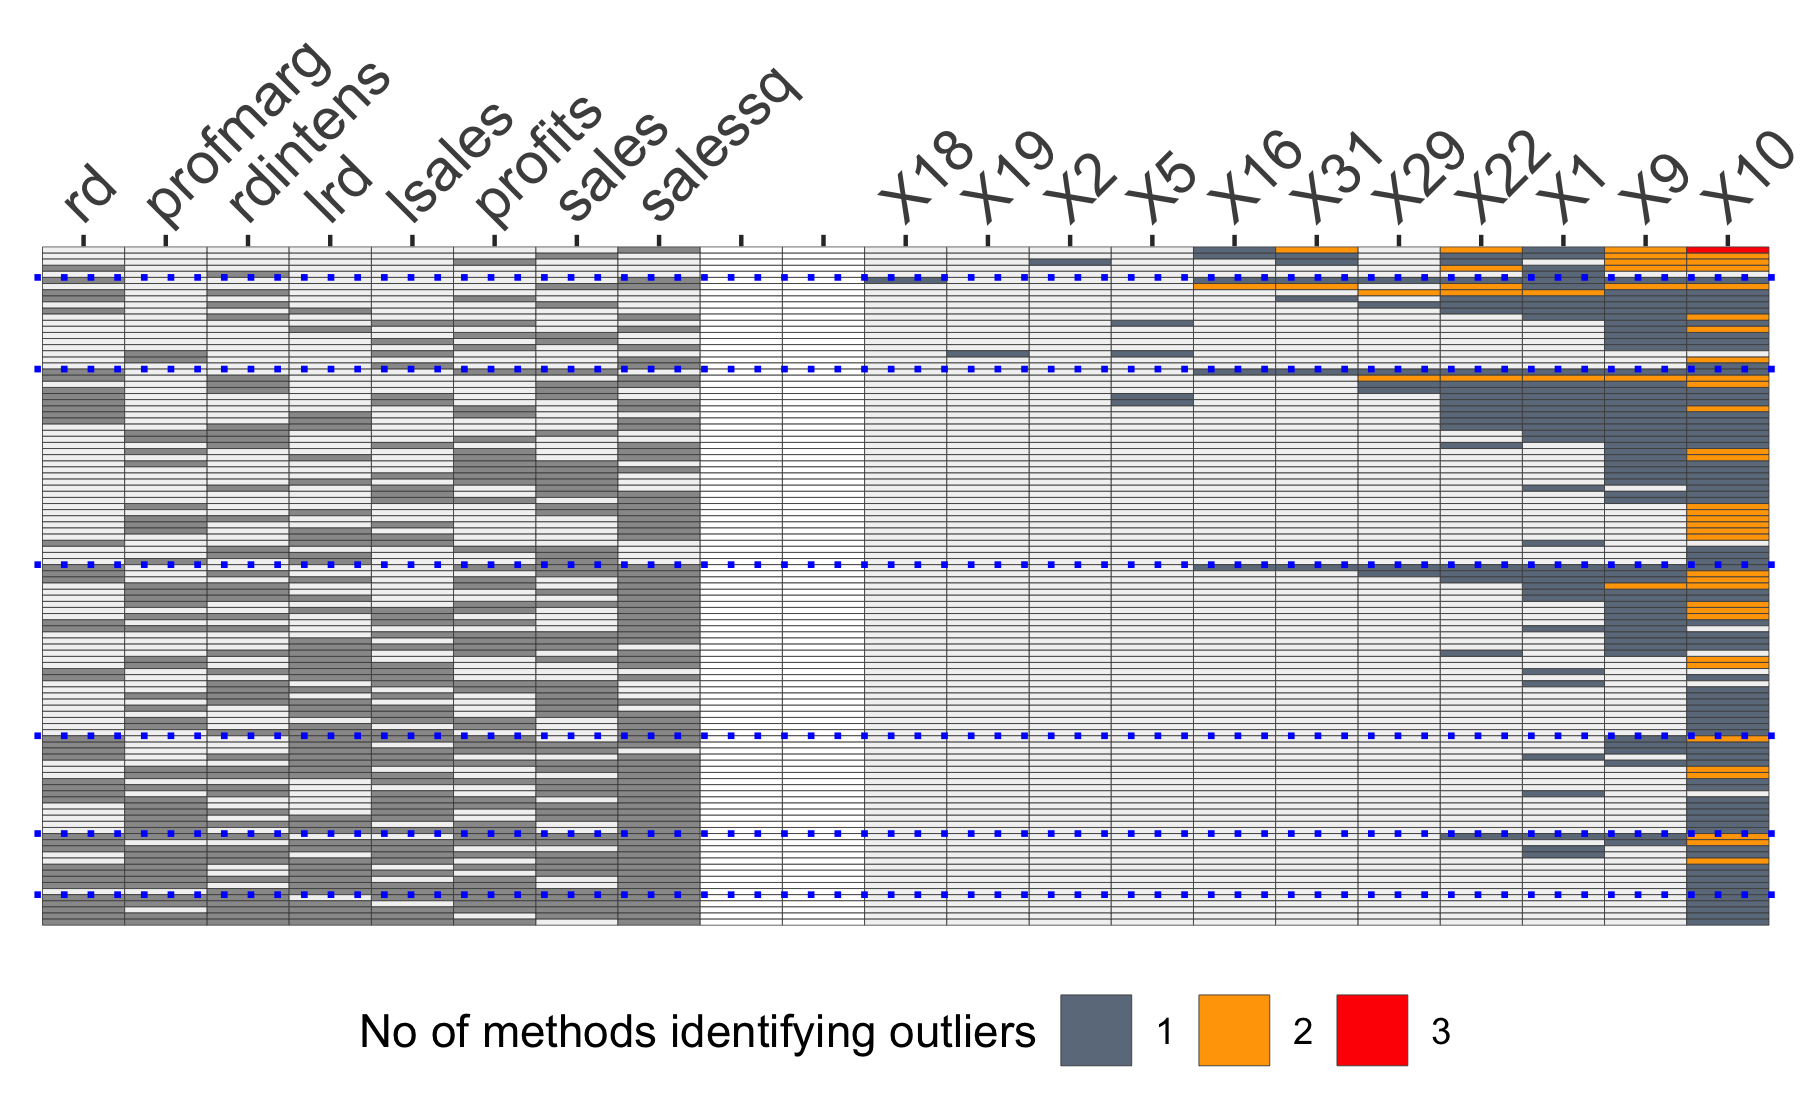
\includegraphics{MEM5220_R_files/figure-latex/unnamed-chunk-140-1.pdf}

\hypertarget{missing-data}{%
\subsubsection{Missing Data}\label{missing-data}}

Missing values in data is a common phenomenon in real world problems. In
R, missing data can be represented by different values of the variable.

\begin{itemize}
\tightlist
\item
  \textbf{NA} (not available) indicates that we do not have the
  information
\item
  \textbf{NaN} (not a number) indicates that the value is not defined,
  for example when we take the log of a negative number
\end{itemize}

Base R offers many functions to detect missing observations. Sometimes
using \textbf{mice} and \textbf{VIM} package for looking at missing data
pattern and imputing missing data is even easier.

\begin{Shaded}
\begin{Highlighting}[]
\KeywordTok{data}\NormalTok{(}\StringTok{"lawsch85"}\NormalTok{, }\DataTypeTok{package =} \StringTok{"wooldridge"}\NormalTok{ )}

\CommentTok{# extract LSAT}
\NormalTok{lsat <-}\StringTok{ }\NormalTok{lawsch85}\OperatorTok{$}\NormalTok{LSAT}

\CommentTok{# Create logical indicator for missings}
\NormalTok{missLSAT <-}\StringTok{ }\KeywordTok{is.na}\NormalTok{(lawsch85}\OperatorTok{$}\NormalTok{LSAT)}

\CommentTok{# LSAT and indicator for Schools No. 120-129:}
\KeywordTok{rbind}\NormalTok{(lsat,missLSAT)[,}\DecValTok{120}\OperatorTok{:}\DecValTok{129}\NormalTok{]}
\end{Highlighting}
\end{Shaded}

\begin{verbatim}
##          [,1] [,2] [,3] [,4] [,5] [,6] [,7] [,8] [,9] [,10]
## lsat      156  159  157  167   NA  158  155  157   NA   163
## missLSAT    0    0    0    0    1    0    0    0    1     0
\end{verbatim}

\begin{Shaded}
\begin{Highlighting}[]
\CommentTok{# Frequencies of indicator}
\KeywordTok{table}\NormalTok{(missLSAT)}
\end{Highlighting}
\end{Shaded}

\begin{verbatim}
## missLSAT
## FALSE  TRUE 
##   150     6
\end{verbatim}

\begin{Shaded}
\begin{Highlighting}[]
\CommentTok{# Missings for all variables in data frame (counts)}
\KeywordTok{colSums}\NormalTok{(}\KeywordTok{is.na}\NormalTok{(lawsch85))}
\end{Highlighting}
\end{Shaded}

\begin{verbatim}
##    rank  salary    cost    LSAT     GPA  libvol faculty     age  clsize 
##       0       8       6       6       7       1       4      45       3 
##   north   south    east    west lsalary studfac   top10  r11_25  r26_40 
##       0       0       0       0       8       6       0       0       0 
##  r41_60 llibvol   lcost 
##       0       1       6
\end{verbatim}

\begin{Shaded}
\begin{Highlighting}[]
\CommentTok{# Indicator for complete cases}
\NormalTok{compl <-}\StringTok{ }\KeywordTok{complete.cases}\NormalTok{(lawsch85)}
\KeywordTok{table}\NormalTok{(compl)}
\end{Highlighting}
\end{Shaded}

\begin{verbatim}
## compl
## FALSE  TRUE 
##    66    90
\end{verbatim}

\begin{Shaded}
\begin{Highlighting}[]
\CommentTok{# MICE package function to display msising values }
\KeywordTok{head}\NormalTok{(}\KeywordTok{md.pattern}\NormalTok{(lawsch85, }\DataTypeTok{plot =} \OtherTok{FALSE}\NormalTok{)) }
\end{Highlighting}
\end{Shaded}

\begin{verbatim}
##    rank north south east west top10 r11_25 r26_40 r41_60 libvol llibvol
## 90    1     1     1    1    1     1      1      1      1      1       1
## 41    1     1     1    1    1     1      1      1      1      1       1
## 6     1     1     1    1    1     1      1      1      1      1       1
## 1     1     1     1    1    1     1      1      1      1      1       1
## 3     1     1     1    1    1     1      1      1      1      1       1
## 1     1     1     1    1    1     1      1      1      1      1       1
##    clsize faculty cost LSAT studfac lcost GPA salary lsalary age  
## 90      1       1    1    1       1     1   1      1       1   1 0
## 41      1       1    1    1       1     1   1      1       1   0 1
## 6       1       1    1    1       1     1   1      0       0   1 2
## 1       1       1    1    1       1     1   1      0       0   0 3
## 3       1       1    1    0       1     1   0      1       1   1 2
## 1       1       1    1    0       1     1   0      1       1   0 3
\end{verbatim}

\begin{Shaded}
\begin{Highlighting}[]
\NormalTok{aggr_plot <-}\StringTok{ }\KeywordTok{aggr}\NormalTok{(lawsch85, }\DataTypeTok{col=}\KeywordTok{c}\NormalTok{(}\StringTok{'navyblue'}\NormalTok{,}\StringTok{'red'}\NormalTok{), }\DataTypeTok{numbers=}\OtherTok{TRUE}\NormalTok{, }\DataTypeTok{sortVars=}\OtherTok{TRUE}\NormalTok{, }\DataTypeTok{labels=}\KeywordTok{names}\NormalTok{(lawsch85), }\DataTypeTok{cex.axis=}\NormalTok{.}\DecValTok{7}\NormalTok{, }\DataTypeTok{gap=}\DecValTok{3}\NormalTok{, }\DataTypeTok{ylab=}\KeywordTok{c}\NormalTok{(}\StringTok{"Histogram of missing data"}\NormalTok{,}\StringTok{"Pattern"}\NormalTok{))}
\end{Highlighting}
\end{Shaded}

\begin{figure}

{\centering 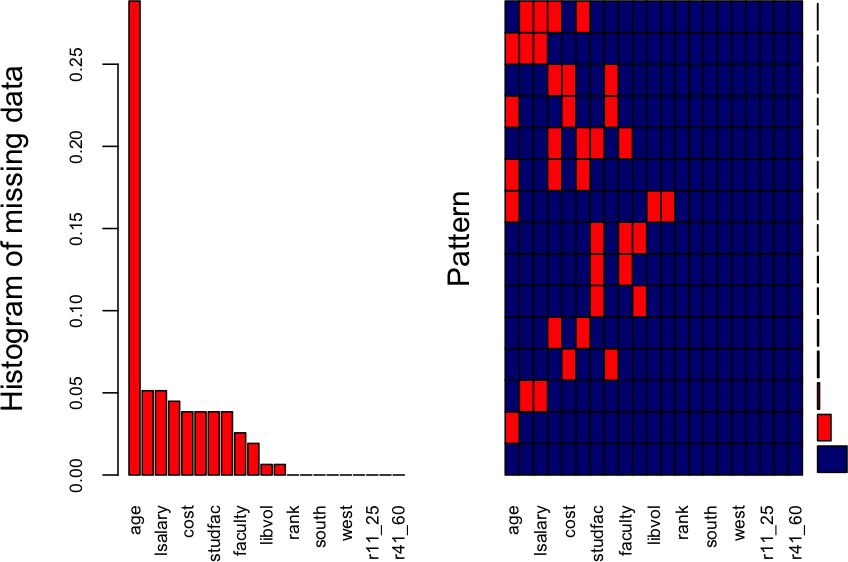
\includegraphics[width=0.8\linewidth]{MEM5220_R_files/figure-latex/fig20-1} 

}

\caption{Visualizing missing data}\label{fig:fig20}
\end{figure}

\begin{verbatim}
## 
##  Variables sorted by number of missings: 
##  Variable       Count
##       age 0.288461538
##    salary 0.051282051
##   lsalary 0.051282051
##       GPA 0.044871795
##      cost 0.038461538
##      LSAT 0.038461538
##   studfac 0.038461538
##     lcost 0.038461538
##   faculty 0.025641026
##    clsize 0.019230769
##    libvol 0.006410256
##   llibvol 0.006410256
##      rank 0.000000000
##     north 0.000000000
##     south 0.000000000
##      east 0.000000000
##      west 0.000000000
##     top10 0.000000000
##    r11_25 0.000000000
##    r26_40 0.000000000
##    r41_60 0.000000000
\end{verbatim}

Regression command like \texttt{lm()} have as argument
\textbf{na.rm=TRUE}!

\begin{Shaded}
\begin{Highlighting}[]
\CommentTok{# Mean of a variable with missings:}
\KeywordTok{mean}\NormalTok{(lawsch85}\OperatorTok{$}\NormalTok{LSAT)}
\end{Highlighting}
\end{Shaded}

\begin{verbatim}
## [1] NA
\end{verbatim}

\begin{Shaded}
\begin{Highlighting}[]
\KeywordTok{mean}\NormalTok{(lawsch85}\OperatorTok{$}\NormalTok{LSAT,}\DataTypeTok{na.rm=}\OtherTok{TRUE}\NormalTok{)}
\end{Highlighting}
\end{Shaded}

\begin{verbatim}
## [1] 158.2933
\end{verbatim}

\begin{Shaded}
\begin{Highlighting}[]
\CommentTok{# Regression with missings}
\KeywordTok{summary}\NormalTok{(}\KeywordTok{lm}\NormalTok{(}\KeywordTok{log}\NormalTok{(salary)}\OperatorTok{~}\NormalTok{LSAT}\OperatorTok{+}\NormalTok{cost}\OperatorTok{+}\NormalTok{age, }\DataTypeTok{data=}\NormalTok{lawsch85))}
\end{Highlighting}
\end{Shaded}

\begin{verbatim}
## 
## Call:
## lm(formula = log(salary) ~ LSAT + cost + age, data = lawsch85)
## 
## Residuals:
##      Min       1Q   Median       3Q      Max 
## -0.40989 -0.09438  0.00317  0.10436  0.45483 
## 
## Coefficients:
##              Estimate Std. Error t value Pr(>|t|)    
## (Intercept) 4.384e+00  6.781e-01   6.465 4.94e-09 ***
## LSAT        3.722e-02  4.501e-03   8.269 1.06e-12 ***
## cost        1.114e-05  4.321e-06   2.577 0.011563 *  
## age         1.503e-03  4.354e-04   3.453 0.000843 ***
## ---
## Signif. codes:  0 '***' 0.001 '**' 0.01 '*' 0.05 '.' 0.1 ' ' 1
## 
## Residual standard error: 0.1545 on 91 degrees of freedom
##   (61 observations deleted due to missingness)
## Multiple R-squared:  0.6708, Adjusted R-squared:  0.6599 
## F-statistic: 61.81 on 3 and 91 DF,  p-value: < 2.2e-16
\end{verbatim}

R packages provide multiple imputation algorithms. Without going into
detail how those algorithms work, we can use for example the
\textbf{meth=``pmm''} argument from the \textbf{mice} package to apply a
predictive mean matching as imputation method.

\begin{Shaded}
\begin{Highlighting}[]
\CommentTok{# We use a diffferent dataset to speed up the imputation process}
\NormalTok{data <-}\StringTok{ }\NormalTok{airquality}
\NormalTok{data[}\DecValTok{4}\OperatorTok{:}\DecValTok{10}\NormalTok{,}\DecValTok{3}\NormalTok{] <-}\StringTok{ }\KeywordTok{rep}\NormalTok{(}\OtherTok{NA}\NormalTok{,}\DecValTok{7}\NormalTok{)}
\NormalTok{data[}\DecValTok{1}\OperatorTok{:}\DecValTok{5}\NormalTok{,}\DecValTok{4}\NormalTok{] <-}\StringTok{ }\OtherTok{NA}
\NormalTok{tempData <-}\StringTok{ }\KeywordTok{mice}\NormalTok{(data,}\DataTypeTok{m=}\DecValTok{5}\NormalTok{,}\DataTypeTok{maxit=}\DecValTok{50}\NormalTok{,}\DataTypeTok{meth=}\StringTok{'pmm'}\NormalTok{,}\DataTypeTok{seed=}\DecValTok{500}\NormalTok{)}
\end{Highlighting}
\end{Shaded}

\begin{Shaded}
\begin{Highlighting}[]
\KeywordTok{summary}\NormalTok{(tempData)}
\end{Highlighting}
\end{Shaded}

\begin{verbatim}
## Class: mids
## Number of multiple imputations:  5 
## Imputation methods:
##   Ozone Solar.R    Wind    Temp   Month     Day 
##   "pmm"   "pmm"   "pmm"   "pmm"      ""      "" 
## PredictorMatrix:
##         Ozone Solar.R Wind Temp Month Day
## Ozone       0       1    1    1     1   1
## Solar.R     1       0    1    1     1   1
## Wind        1       1    0    1     1   1
## Temp        1       1    1    0     1   1
## Month       1       1    1    1     0   1
## Day         1       1    1    1     1   0
\end{verbatim}

\hypertarget{least-absolute-deviations-lad-estimation}{%
\section{Least absolute Deviations (LAD)
Estimation}\label{least-absolute-deviations-lad-estimation}}

As an alternative to OLS, the least absolute deviations (LAD) is less
sensitive to outliers. Instead of minimizing the sum of \emph{squared}
residuals, it minimizes the sum of the \emph{absolute values} of the
residuals.

In R, general quantile regression (and LAD as the default special case)
can easily be implemented with the command \texttt{reg()} from the
\textbf{quantreg} package.

\begin{Shaded}
\begin{Highlighting}[]
\CommentTok{# OLS Regression}
\NormalTok{ols <-}\StringTok{ }\KeywordTok{lm}\NormalTok{(rdintens }\OperatorTok{~}\StringTok{ }\KeywordTok{I}\NormalTok{(sales}\OperatorTok{/}\DecValTok{1000}\NormalTok{) }\OperatorTok{+}\NormalTok{profmarg, }\DataTypeTok{data=}\NormalTok{rdchem)}
\CommentTok{# LAD Regression}
\NormalTok{lad <-}\StringTok{ }\KeywordTok{rq}\NormalTok{(rdintens }\OperatorTok{~}\StringTok{ }\KeywordTok{I}\NormalTok{(sales}\OperatorTok{/}\DecValTok{1000}\NormalTok{) }\OperatorTok{+}\NormalTok{profmarg, }\DataTypeTok{data=}\NormalTok{rdchem)}

\CommentTok{# regression table}
\KeywordTok{stargazer}\NormalTok{(ols,lad,  }\DataTypeTok{type =} \StringTok{"text"}\NormalTok{)}
\end{Highlighting}
\end{Shaded}

\begin{verbatim}
## 
## =================================================
##                          Dependent variable:     
##                     -----------------------------
##                               rdintens           
##                            OLS          quantile 
##                                        regression
##                            (1)            (2)    
## -------------------------------------------------
## I(sales/1000)             0.053          0.019   
##                          (0.044)        (0.059)  
##                                                  
## profmarg                  0.045         0.118**  
##                          (0.046)        (0.049)  
##                                                  
## Constant                 2.625***       1.623*** 
##                          (0.586)        (0.509)  
##                                                  
## -------------------------------------------------
## Observations                32             32    
## R2                        0.076                  
## Adjusted R2               0.012                  
## Residual Std. Error  1.862 (df = 29)             
## F Statistic         1.195 (df = 2; 29)           
## =================================================
## Note:                 *p<0.1; **p<0.05; ***p<0.01
\end{verbatim}

Note: LAD inferences are only valid asymptotically, so the results in
this example with \(n =32\) should be taken with caution.

\hypertarget{binarymodels}{%
\chapter{Qualitative and LDV Models}\label{binarymodels}}

To load the dataset and necessary functions:

\begin{Shaded}
\begin{Highlighting}[]
\CommentTok{# This function 1. checks if the packages are installed. 2. It installs the packages if they were not in the list of installed packages. 3. It loads the packages into the workspace}
\CommentTok{# devtools::install_github("ccolonescu/PoEdata")}
\NormalTok{PACKAGES<-}\KeywordTok{c}\NormalTok{(}
            \StringTok{"tidyverse"}\NormalTok{,  }\CommentTok{# for data manipulation and ggplots}
            \StringTok{"broom"}\NormalTok{,  }\CommentTok{# Tidy regression output}
            \StringTok{"Hmisc"}\NormalTok{, }\CommentTok{# Harrell Miscellaneous functions}
            \StringTok{"psych"}\NormalTok{, }\CommentTok{# Procedures for Psychometric research}
            \StringTok{"car"}\NormalTok{, }\CommentTok{# Companion to applied regression}
            \StringTok{"knitr"}\NormalTok{, }\CommentTok{# knit functions}
            \CommentTok{# "kableExtra", # extended knit functions for objects exported from other packages}
            \StringTok{"huxtable"}\NormalTok{, }\CommentTok{#  Regression tables, broom compatible}
            \StringTok{"stargazer"}\NormalTok{, }\CommentTok{# Regression tables}
            \StringTok{"AER"}\NormalTok{, }\CommentTok{#  Functions, data sets, examples, demos, and vignettes for the book Christian Kleiber and Achim Zeileis (2008)}
            \StringTok{"PoEdata"}\NormalTok{, }\CommentTok{# R data sets for "Principles of Econometrics" by Hill, Griffiths, and Lim, 4e, Wiley. https://github.com/ccolonescu/PoEdata}
            \StringTok{"wooldridge"}\NormalTok{,  }\CommentTok{# Wooldrige Datasets}
            \StringTok{"MCMCpack"}\NormalTok{, }\CommentTok{# Contains functions to perform Bayesian inference using posterior simulation for a number of ssatistical models.}
            \StringTok{"sampleSelection"}\NormalTok{, }\CommentTok{# Two-step and maximum likelihood estimation of Heckman-type sample selection models}
            \StringTok{"scales"}\NormalTok{, }\CommentTok{# scale helper functions such as percent }
            \StringTok{"lmtest"}\NormalTok{, }
            \StringTok{"margins"}\NormalTok{, }\CommentTok{# Stata like margin functions}
            \StringTok{"prediction"}\NormalTok{, }\CommentTok{# Type stable predictions}
            \StringTok{"nnet"}\NormalTok{, }\CommentTok{# Multinomial logit}
            \StringTok{"survival"}\NormalTok{, }\CommentTok{# Survival Analysis}
            \StringTok{"sampleSelection"}\NormalTok{, }\CommentTok{# Heckman type sample selection}
            \StringTok{"censReg"}\NormalTok{, }\CommentTok{# Censored Regression models}
            \StringTok{"magrittr"}\NormalTok{) }\CommentTok{#  pipes}
\NormalTok{inst<-}\KeywordTok{match}\NormalTok{(PACKAGES, }\KeywordTok{.packages}\NormalTok{(}\DataTypeTok{all=}\OtherTok{TRUE}\NormalTok{))}
\NormalTok{need<-}\KeywordTok{which}\NormalTok{(}\KeywordTok{is.na}\NormalTok{(inst))}
\ControlFlowTok{if}\NormalTok{ (}\KeywordTok{length}\NormalTok{(need)}\OperatorTok{>}\DecValTok{0}\NormalTok{) }\KeywordTok{install.packages}\NormalTok{(PACKAGES[need])}
\KeywordTok{lapply}\NormalTok{(PACKAGES, require, }\DataTypeTok{character.only=}\NormalTok{T)}
\end{Highlighting}
\end{Shaded}

Binary dependent variables are frequently studied in applied economics.
Because a dummy variable \(y\) can only take values 0 and 1, its
(conditional) expected value is equal to the (conditional) probability
that \(y=1\):

\(E(y|x) = 0 \times P(y = 0|x) + 1 \times P(y = 1|x) = P(y=1|x)\)

An important class of models specifies the success probability as

\(P(y = 1 | x) = G(\beta_0 + \beta_1 + \dots \beta_k x_k) = G(\boldsymbol{x} \boldsymbol{\beta})\)

The following table is taken from \citet{dalpiaz2016} and summarizes
three examples of a generalized linear model:

\begin{longtable}[]{@{}llll@{}}
\toprule
\begin{minipage}[b]{0.20\columnwidth}\raggedright
\strut
\end{minipage} & \begin{minipage}[b]{0.21\columnwidth}\raggedright
Linear Regression\strut
\end{minipage} & \begin{minipage}[b]{0.23\columnwidth}\raggedright
Poisson Regression\strut
\end{minipage} & \begin{minipage}[b]{0.24\columnwidth}\raggedright
Logistic Regression\strut
\end{minipage}\tabularnewline
\midrule
\endhead
\begin{minipage}[t]{0.20\columnwidth}\raggedright
\(Y \mid {\bf X} = {\bf x}\)\strut
\end{minipage} & \begin{minipage}[t]{0.21\columnwidth}\raggedright
\(N(\mu({\bf x}), \sigma^2)\)\strut
\end{minipage} & \begin{minipage}[t]{0.23\columnwidth}\raggedright
\(\text{Pois}(\lambda({\bf x}))\)\strut
\end{minipage} & \begin{minipage}[t]{0.24\columnwidth}\raggedright
\(\text{Bern}(p({\bf x}))\)\strut
\end{minipage}\tabularnewline
\begin{minipage}[t]{0.20\columnwidth}\raggedright
\textbf{Distribution Name}\strut
\end{minipage} & \begin{minipage}[t]{0.21\columnwidth}\raggedright
Normal\strut
\end{minipage} & \begin{minipage}[t]{0.23\columnwidth}\raggedright
Poisson\strut
\end{minipage} & \begin{minipage}[t]{0.24\columnwidth}\raggedright
Bernoulli (Binomial)\strut
\end{minipage}\tabularnewline
\begin{minipage}[t]{0.20\columnwidth}\raggedright
\(\text{E}[Y \mid {\bf X} = {\bf x}]\)\strut
\end{minipage} & \begin{minipage}[t]{0.21\columnwidth}\raggedright
\(\mu({\bf x})\)\strut
\end{minipage} & \begin{minipage}[t]{0.23\columnwidth}\raggedright
\(\lambda({\bf x})\)\strut
\end{minipage} & \begin{minipage}[t]{0.24\columnwidth}\raggedright
\(p({\bf x})\)\strut
\end{minipage}\tabularnewline
\begin{minipage}[t]{0.20\columnwidth}\raggedright
\textbf{Support}\strut
\end{minipage} & \begin{minipage}[t]{0.21\columnwidth}\raggedright
Real: \((-\infty, \infty)\)\strut
\end{minipage} & \begin{minipage}[t]{0.23\columnwidth}\raggedright
Integer: \(0, 1, 2, \ldots\)\strut
\end{minipage} & \begin{minipage}[t]{0.24\columnwidth}\raggedright
Integer: \(0, 1\)\strut
\end{minipage}\tabularnewline
\begin{minipage}[t]{0.20\columnwidth}\raggedright
\textbf{Usage}\strut
\end{minipage} & \begin{minipage}[t]{0.21\columnwidth}\raggedright
Numeric Data\strut
\end{minipage} & \begin{minipage}[t]{0.23\columnwidth}\raggedright
Count (Integer) Data\strut
\end{minipage} & \begin{minipage}[t]{0.24\columnwidth}\raggedright
Binary (Class ) Data\strut
\end{minipage}\tabularnewline
\begin{minipage}[t]{0.20\columnwidth}\raggedright
\textbf{Link Name}\strut
\end{minipage} & \begin{minipage}[t]{0.21\columnwidth}\raggedright
Identity\strut
\end{minipage} & \begin{minipage}[t]{0.23\columnwidth}\raggedright
Log\strut
\end{minipage} & \begin{minipage}[t]{0.24\columnwidth}\raggedright
Logit\strut
\end{minipage}\tabularnewline
\begin{minipage}[t]{0.20\columnwidth}\raggedright
\textbf{Link Function}\strut
\end{minipage} & \begin{minipage}[t]{0.21\columnwidth}\raggedright
\(\eta({\bf x}) = \mu({\bf x})\)\strut
\end{minipage} & \begin{minipage}[t]{0.23\columnwidth}\raggedright
\(\eta({\bf x}) = \log(\lambda({\bf x}))\)\strut
\end{minipage} & \begin{minipage}[t]{0.24\columnwidth}\raggedright
\(\eta({\bf x}) = \log \left(\frac{p({\bf x})}{1 - p({\bf x})} \right)\)\strut
\end{minipage}\tabularnewline
\begin{minipage}[t]{0.20\columnwidth}\raggedright
\textbf{Mean Function}\strut
\end{minipage} & \begin{minipage}[t]{0.21\columnwidth}\raggedright
\(\mu({\bf x}) = \eta({\bf x})\)\strut
\end{minipage} & \begin{minipage}[t]{0.23\columnwidth}\raggedright
\(\lambda({\bf x}) = e^{\eta({\bf x})}\)\strut
\end{minipage} & \begin{minipage}[t]{0.24\columnwidth}\raggedright
\(p({\bf x}) = \frac{e^{\eta({\bf x})}}{1 + e^{\eta({\bf x})}} = \frac{1}{1 + e^{-\eta({\bf x})}}\)\strut
\end{minipage}\tabularnewline
\bottomrule
\end{longtable}

Like ordinary linear regression, we will seek to ``fit'' the model by
estimating the \(\beta\) parameters. To do so, we will use the method of
maximum likelihood.

Note that a Bernoulli distribution is a specific case of a binomial
distribution where the \(n\) parameter of a binomial is \(1\). Binomial
regression is also possible, but we'll focus on the much more popular
Bernoulli case.

So, in general, GLMs relate the mean of the response to a linear
combination of the predictors, \(\eta({\bf x})\), through the use of a
link function, \(g()\). That is,

\[
\eta({\bf x}) = g\left(\text{E}[Y \mid {\bf X} = {\bf x}]\right).
\]

The mean is then

\[
\text{E}[Y \mid {\bf X} = {\bf x}] = g^{-1}(\eta({\bf x})).
\]

\hypertarget{linear-probability-models}{%
\section{Linear probability models}\label{linear-probability-models}}

If a dummy variable is used as the dependent variable \(y\), we can
still use OLS to estimate its relation to the regressors \(x\).

\begin{Shaded}
\begin{Highlighting}[]
\KeywordTok{data}\NormalTok{(}\StringTok{"mroz"}\NormalTok{, }\DataTypeTok{package =} \StringTok{"wooldridge"}\NormalTok{)}
\end{Highlighting}
\end{Shaded}

Let us use the \texttt{describe()} function from the \textbf{Hmisc}
package to use a different way to describe the datatset.

\begin{Shaded}
\begin{Highlighting}[]
\KeywordTok{describe}\NormalTok{(mroz)}
\end{Highlighting}
\end{Shaded}

\textbackslash{}begin\{table\}{[}h{]}
\textbackslash{}begin\{raggedright\}

\providecommand{\huxb}[2][0,0,0]{\arrayrulecolor[RGB]{#1}\global\arrayrulewidth=#2pt}
    \providecommand{\huxvb}[2][0,0,0]{\color[RGB]{#1}\vrule width #2pt}
    \providecommand{\huxtpad}[1]{\rule{0pt}{\baselineskip+#1}}
    \providecommand{\huxbpad}[1]{\rule[-#1]{0pt}{#1}}
  \begin{tabularx}{1\textwidth}{p{0.0769230769230769\textwidth} p{0.0769230769230769\textwidth} p{0.0769230769230769\textwidth} p{0.0769230769230769\textwidth} p{0.0769230769230769\textwidth} p{0.0769230769230769\textwidth} p{0.0769230769230769\textwidth} p{0.0769230769230769\textwidth} p{0.0769230769230769\textwidth} p{0.0769230769230769\textwidth} p{0.0769230769230769\textwidth} p{0.0769230769230769\textwidth} p{0.0769230769230769\textwidth}}


\par

\textbackslash{}end\{raggedright\} \textbackslash{}end\{table\}

The function \texttt{rcorr()} can be useful to check visually for
correlation.

\begin{Shaded}
\begin{Highlighting}[]
\KeywordTok{rcorr}\NormalTok{(}\KeywordTok{as.matrix}\NormalTok{(mroz))}
\end{Highlighting}
\end{Shaded}

\begin{verbatim}
##           inlf hours kidslt6 kidsge6   age  educ  wage repwage hushrs
## inlf      1.00  0.74   -0.21    0.00 -0.08  0.19   NaN    0.63  -0.07
## hours     0.74  1.00   -0.22   -0.09 -0.03  0.11 -0.10    0.61  -0.06
## kidslt6  -0.21 -0.22    1.00    0.08 -0.43  0.11  0.03   -0.13   0.02
## kidsge6   0.00 -0.09    0.08    1.00 -0.39 -0.06 -0.08   -0.07   0.10
## age      -0.08 -0.03   -0.43   -0.39  1.00 -0.12  0.03   -0.06  -0.08
## educ      0.19  0.11    0.11   -0.06 -0.12  1.00  0.34    0.27   0.08
## wage       NaN -0.10    0.03   -0.08  0.03  0.34  1.00    0.42  -0.03
## repwage   0.63  0.61   -0.13   -0.07 -0.06  0.27  0.42    1.00  -0.07
## hushrs   -0.07 -0.06    0.02    0.10 -0.08  0.08 -0.03   -0.07   1.00
## husage   -0.07 -0.03   -0.44   -0.35  0.89 -0.13  0.03   -0.06  -0.10
## huseduc   0.05 -0.01    0.13    0.01 -0.16  0.61  0.17    0.11   0.11
## huswage  -0.07 -0.10    0.03   -0.03  0.03  0.28  0.22    0.02  -0.24
## faminc    0.10  0.15   -0.03   -0.02  0.05  0.36  0.30    0.21   0.13
## mtr      -0.14 -0.19    0.06    0.15 -0.06 -0.41 -0.31   -0.24  -0.14
## motheduc  0.09  0.06    0.11    0.03 -0.23  0.44  0.06    0.09   0.05
## fatheduc  0.06  0.01    0.10   -0.03 -0.16  0.44  0.11    0.10   0.05
## unem     -0.03 -0.06   -0.01    0.01  0.08  0.07  0.03    0.01  -0.16
## city     -0.01 -0.02   -0.04   -0.03  0.10  0.16  0.12    0.09  -0.11
## exper     0.34  0.40   -0.19   -0.30  0.33  0.07  0.05    0.34  -0.10
## nwifeinc -0.12 -0.12    0.04    0.02  0.06  0.28  0.14   -0.06   0.16
## lwage      NaN -0.02   -0.02   -0.12  0.05  0.34  0.83    0.51   0.00
## expersq   0.26  0.34   -0.18   -0.30  0.38  0.02  0.04    0.28  -0.07
##          husage huseduc huswage faminc   mtr motheduc fatheduc  unem  city
## inlf      -0.07    0.05   -0.07   0.10 -0.14     0.09     0.06 -0.03 -0.01
## hours     -0.03   -0.01   -0.10   0.15 -0.19     0.06     0.01 -0.06 -0.02
## kidslt6   -0.44    0.13    0.03  -0.03  0.06     0.11     0.10 -0.01 -0.04
## kidsge6   -0.35    0.01   -0.03  -0.02  0.15     0.03    -0.03  0.01 -0.03
## age        0.89   -0.16    0.03   0.05 -0.06    -0.23    -0.16  0.08  0.10
## educ      -0.13    0.61    0.28   0.36 -0.41     0.44     0.44  0.07  0.16
## wage       0.03    0.17    0.22   0.30 -0.31     0.06     0.11  0.03  0.12
## repwage   -0.06    0.11    0.02   0.21 -0.24     0.09     0.10  0.01  0.09
## hushrs    -0.10    0.11   -0.24   0.13 -0.14     0.05     0.05 -0.16 -0.11
## husage     1.00   -0.20    0.02   0.04 -0.04    -0.23    -0.14  0.05  0.07
## huseduc   -0.20    1.00    0.39   0.38 -0.44     0.32     0.37  0.06  0.23
## huswage    0.02    0.39    1.00   0.73 -0.72     0.13     0.19  0.16  0.32
## faminc     0.04    0.38    0.73   1.00 -0.88     0.16     0.21  0.06  0.25
## mtr       -0.04   -0.44   -0.72  -0.88  1.00    -0.19    -0.25 -0.06 -0.26
## motheduc  -0.23    0.32    0.13   0.16 -0.19     1.00     0.57  0.02  0.07
## fatheduc  -0.14    0.37    0.19   0.21 -0.25     0.57     1.00  0.06  0.15
## unem       0.05    0.06    0.16   0.06 -0.06     0.02     0.06  1.00  0.18
## city       0.07    0.23    0.32   0.25 -0.26     0.07     0.15  0.18  1.00
## exper      0.27   -0.04   -0.10  -0.03 -0.03    -0.08    -0.08  0.00  0.01
## nwifeinc   0.05    0.36    0.76   0.94 -0.81     0.13     0.19  0.07  0.24
## lwage      0.04    0.16    0.17   0.35 -0.37     0.05     0.08  0.04  0.10
## expersq    0.31   -0.07   -0.12  -0.04 -0.02    -0.10    -0.10 -0.02 -0.01
##          exper nwifeinc lwage expersq
## inlf      0.34    -0.12   NaN    0.26
## hours     0.40    -0.12 -0.02    0.34
## kidslt6  -0.19     0.04 -0.02   -0.18
## kidsge6  -0.30     0.02 -0.12   -0.30
## age       0.33     0.06  0.05    0.38
## educ      0.07     0.28  0.34    0.02
## wage      0.05     0.14  0.83    0.04
## repwage   0.34    -0.06  0.51    0.28
## hushrs   -0.10     0.16  0.00   -0.07
## husage    0.27     0.05  0.04    0.31
## huseduc  -0.04     0.36  0.16   -0.07
## huswage  -0.10     0.76  0.17   -0.12
## faminc   -0.03     0.94  0.35   -0.04
## mtr      -0.03    -0.81 -0.37   -0.02
## motheduc -0.08     0.13  0.05   -0.10
## fatheduc -0.08     0.19  0.08   -0.10
## unem      0.00     0.07  0.04   -0.02
## city      0.01     0.24  0.10   -0.01
## exper     1.00    -0.17  0.17    0.94
## nwifeinc -0.17     1.00  0.14   -0.17
## lwage     0.17     0.14  1.00    0.13
## expersq   0.94    -0.17  0.13    1.00
## 
## n
##          inlf hours kidslt6 kidsge6 age educ wage repwage hushrs husage
## inlf      753   753     753     753 753  753  428     753    753    753
## hours     753   753     753     753 753  753  428     753    753    753
## kidslt6   753   753     753     753 753  753  428     753    753    753
## kidsge6   753   753     753     753 753  753  428     753    753    753
## age       753   753     753     753 753  753  428     753    753    753
## educ      753   753     753     753 753  753  428     753    753    753
## wage      428   428     428     428 428  428  428     428    428    428
## repwage   753   753     753     753 753  753  428     753    753    753
## hushrs    753   753     753     753 753  753  428     753    753    753
## husage    753   753     753     753 753  753  428     753    753    753
## huseduc   753   753     753     753 753  753  428     753    753    753
## huswage   753   753     753     753 753  753  428     753    753    753
## faminc    753   753     753     753 753  753  428     753    753    753
## mtr       753   753     753     753 753  753  428     753    753    753
## motheduc  753   753     753     753 753  753  428     753    753    753
## fatheduc  753   753     753     753 753  753  428     753    753    753
## unem      753   753     753     753 753  753  428     753    753    753
## city      753   753     753     753 753  753  428     753    753    753
## exper     753   753     753     753 753  753  428     753    753    753
## nwifeinc  753   753     753     753 753  753  428     753    753    753
## lwage     428   428     428     428 428  428  428     428    428    428
## expersq   753   753     753     753 753  753  428     753    753    753
##          huseduc huswage faminc mtr motheduc fatheduc unem city exper
## inlf         753     753    753 753      753      753  753  753   753
## hours        753     753    753 753      753      753  753  753   753
## kidslt6      753     753    753 753      753      753  753  753   753
## kidsge6      753     753    753 753      753      753  753  753   753
## age          753     753    753 753      753      753  753  753   753
## educ         753     753    753 753      753      753  753  753   753
## wage         428     428    428 428      428      428  428  428   428
## repwage      753     753    753 753      753      753  753  753   753
## hushrs       753     753    753 753      753      753  753  753   753
## husage       753     753    753 753      753      753  753  753   753
## huseduc      753     753    753 753      753      753  753  753   753
## huswage      753     753    753 753      753      753  753  753   753
## faminc       753     753    753 753      753      753  753  753   753
## mtr          753     753    753 753      753      753  753  753   753
## motheduc     753     753    753 753      753      753  753  753   753
## fatheduc     753     753    753 753      753      753  753  753   753
## unem         753     753    753 753      753      753  753  753   753
## city         753     753    753 753      753      753  753  753   753
## exper        753     753    753 753      753      753  753  753   753
## nwifeinc     753     753    753 753      753      753  753  753   753
## lwage        428     428    428 428      428      428  428  428   428
## expersq      753     753    753 753      753      753  753  753   753
##          nwifeinc lwage expersq
## inlf          753   428     753
## hours         753   428     753
## kidslt6       753   428     753
## kidsge6       753   428     753
## age           753   428     753
## educ          753   428     753
## wage          428   428     428
## repwage       753   428     753
## hushrs        753   428     753
## husage        753   428     753
## huseduc       753   428     753
## huswage       753   428     753
## faminc        753   428     753
## mtr           753   428     753
## motheduc      753   428     753
## fatheduc      753   428     753
## unem          753   428     753
## city          753   428     753
## exper         753   428     753
## nwifeinc      753   428     753
## lwage         428   428     428
## expersq       753   428     753
## 
## P
##          inlf   hours  kidslt6 kidsge6 age    educ   wage   repwage hushrs
## inlf            0.0000 0.0000  0.9470  0.0272 0.0000        0.0000  0.0738
## hours    0.0000        0.0000  0.0128  0.3642 0.0036 0.0435 0.0000  0.1224
## kidslt6  0.0000 0.0000         0.0209  0.0000 0.0028 0.5168 0.0002  0.5057
## kidsge6  0.9470 0.0128 0.0209          0.0000 0.1063 0.1017 0.0596  0.0063
## age      0.0272 0.3642 0.0000  0.0000         0.0009 0.5306 0.1098  0.0206
## educ     0.0000 0.0036 0.0028  0.1063  0.0009        0.0000 0.0000  0.0304
## wage            0.0435 0.5168  0.1017  0.5306 0.0000        0.0000  0.5061
## repwage  0.0000 0.0000 0.0002  0.0596  0.1098 0.0000 0.0000         0.0521
## hushrs   0.0738 0.1224 0.5057  0.0063  0.0206 0.0304 0.5061 0.0521        
## husage   0.0458 0.3943 0.0000  0.0000  0.0000 0.0002 0.5966 0.1288  0.0088
## huseduc  0.2082 0.7915 0.0002  0.7960  0.0000 0.0000 0.0006 0.0033  0.0030
## huswage  0.0567 0.0068 0.3749  0.4156  0.4592 0.0000 0.0000 0.5974  0.0000
## faminc   0.0066 0.0000 0.4465  0.5930  0.1505 0.0000 0.0000 0.0000  0.0004
## mtr      0.0000 0.0000 0.1010  0.0000  0.1037 0.0000 0.0000 0.0000  0.0002
## motheduc 0.0130 0.1126 0.0031  0.3749  0.0000 0.0000 0.2387 0.0188  0.1436
## fatheduc 0.1135 0.7080 0.0083  0.4622  0.0000 0.0000 0.0258 0.0048  0.1676
## unem     0.4311 0.0983 0.8042  0.6956  0.0345 0.0478 0.5054 0.8026  0.0000
## city     0.8658 0.6568 0.2426  0.3577  0.0081 0.0000 0.0135 0.0164  0.0020
## exper    0.0000 0.0000 0.0000  0.0000  0.0000 0.0692 0.2563 0.0000  0.0064
## nwifeinc 0.0012 0.0006 0.2951  0.4974  0.1078 0.0000 0.0032 0.1258  0.0000
## lwage           0.7315 0.7026  0.0130  0.2569 0.0000 0.0000 0.0000  0.9378
## expersq  0.0000 0.0000 0.0000  0.0000  0.0000 0.5084 0.3814 0.0000  0.0406
##          husage huseduc huswage faminc mtr    motheduc fatheduc unem  
## inlf     0.0458 0.2082  0.0567  0.0066 0.0000 0.0130   0.1135   0.4311
## hours    0.3943 0.7915  0.0068  0.0000 0.0000 0.1126   0.7080   0.0983
## kidslt6  0.0000 0.0002  0.3749  0.4465 0.1010 0.0031   0.0083   0.8042
## kidsge6  0.0000 0.7960  0.4156  0.5930 0.0000 0.3749   0.4622   0.6956
## age      0.0000 0.0000  0.4592  0.1505 0.1037 0.0000   0.0000   0.0345
## educ     0.0002 0.0000  0.0000  0.0000 0.0000 0.0000   0.0000   0.0478
## wage     0.5966 0.0006  0.0000  0.0000 0.0000 0.2387   0.0258   0.5054
## repwage  0.1288 0.0033  0.5974  0.0000 0.0000 0.0188   0.0048   0.8026
## hushrs   0.0088 0.0030  0.0000  0.0004 0.0002 0.1436   0.1676   0.0000
## husage          0.0000  0.5897  0.2670 0.2214 0.0000   0.0002   0.1455
## huseduc  0.0000         0.0000  0.0000 0.0000 0.0000   0.0000   0.1315
## huswage  0.5897 0.0000          0.0000 0.0000 0.0005   0.0000   0.0000
## faminc   0.2670 0.0000  0.0000         0.0000 0.0000   0.0000   0.0916
## mtr      0.2214 0.0000  0.0000  0.0000        0.0000   0.0000   0.1138
## motheduc 0.0000 0.0000  0.0005  0.0000 0.0000          0.0000   0.6141
## fatheduc 0.0002 0.0000  0.0000  0.0000 0.0000 0.0000            0.1085
## unem     0.1455 0.1315  0.0000  0.0916 0.1138 0.6141   0.1085         
## city     0.0636 0.0000  0.0000  0.0000 0.0000 0.0623   0.0000   0.0000
## exper    0.0000 0.3198  0.0045  0.4478 0.3725 0.0241   0.0306   0.9033
## nwifeinc 0.2091 0.0000  0.0000  0.0000 0.0000 0.0004   0.0000   0.0398
## lwage    0.4211 0.0010  0.0005  0.0000 0.0000 0.3305   0.1086   0.3933
## expersq  0.0000 0.0413  0.0011  0.2458 0.6564 0.0060   0.0068   0.5108
##          city   exper  nwifeinc lwage  expersq
## inlf     0.8658 0.0000 0.0012          0.0000 
## hours    0.6568 0.0000 0.0006   0.7315 0.0000 
## kidslt6  0.2426 0.0000 0.2951   0.7026 0.0000 
## kidsge6  0.3577 0.0000 0.4974   0.0130 0.0000 
## age      0.0081 0.0000 0.1078   0.2569 0.0000 
## educ     0.0000 0.0692 0.0000   0.0000 0.5084 
## wage     0.0135 0.2563 0.0032   0.0000 0.3814 
## repwage  0.0164 0.0000 0.1258   0.0000 0.0000 
## hushrs   0.0020 0.0064 0.0000   0.9378 0.0406 
## husage   0.0636 0.0000 0.2091   0.4211 0.0000 
## huseduc  0.0000 0.3198 0.0000   0.0010 0.0413 
## huswage  0.0000 0.0045 0.0000   0.0005 0.0011 
## faminc   0.0000 0.4478 0.0000   0.0000 0.2458 
## mtr      0.0000 0.3725 0.0000   0.0000 0.6564 
## motheduc 0.0623 0.0241 0.0004   0.3305 0.0060 
## fatheduc 0.0000 0.0306 0.0000   0.1086 0.0068 
## unem     0.0000 0.9033 0.0398   0.3933 0.5108 
## city            0.7583 0.0000   0.0446 0.7565 
## exper    0.7583        0.0000   0.0004 0.0000 
## nwifeinc 0.0000 0.0000          0.0034 0.0000 
## lwage    0.0446 0.0004 0.0034          0.0090 
## expersq  0.7565 0.0000 0.0000   0.0090
\end{verbatim}

Estimate linear probability model

\begin{Shaded}
\begin{Highlighting}[]
\NormalTok{linprob <-}\StringTok{ }\KeywordTok{lm}\NormalTok{(inlf}\OperatorTok{~}\NormalTok{nwifeinc}\OperatorTok{+}\NormalTok{educ}\OperatorTok{+}\NormalTok{exper}\OperatorTok{+}\KeywordTok{I}\NormalTok{(exper}\OperatorTok{^}\DecValTok{2}\NormalTok{)}\OperatorTok{+}\NormalTok{age}\OperatorTok{+}\NormalTok{kidslt6}\OperatorTok{+}\NormalTok{kidsge6,}\DataTypeTok{data=}\NormalTok{mroz)}
\CommentTok{# Regression table with heteroscedasticity-robust SE and t tests:}
\KeywordTok{coeftest}\NormalTok{(linprob,}\DataTypeTok{vcov=}\NormalTok{hccm)}
\end{Highlighting}
\end{Shaded}

\begin{verbatim}
## 
## t test of coefficients:
## 
##                Estimate  Std. Error t value  Pr(>|t|)    
## (Intercept)  0.58551922  0.15358032  3.8125  0.000149 ***
## nwifeinc    -0.00340517  0.00155826 -2.1852  0.029182 *  
## educ         0.03799530  0.00733982  5.1766 2.909e-07 ***
## exper        0.03949239  0.00598359  6.6001 7.800e-11 ***
## I(exper^2)  -0.00059631  0.00019895 -2.9973  0.002814 ** 
## age         -0.01609081  0.00241459 -6.6640 5.183e-11 ***
## kidslt6     -0.26181047  0.03215160 -8.1430 1.621e-15 ***
## kidsge6      0.01301223  0.01366031  0.9526  0.341123    
## ---
## Signif. codes:  0 '***' 0.001 '**' 0.01 '*' 0.05 '.' 0.1 ' ' 1
\end{verbatim}

The estimated coefficient \emph{educ} can be interpreted as: an
additional year of schooling increases the probability that a woman is
in the labor force \emph{ceteris paribus} by 3.80\%.

One problem with linear probability models is that \(P(y=1|x)\) is
specified as a linear function of the regressors. By construction, there
are more or less realistic combinations of regressor values that yield
\(\hat{y} < 0\) or \(\hat{y} > 1\).

Predictions for two ``extreme'' women:

\begin{Shaded}
\begin{Highlighting}[]
\NormalTok{xpred <-}\StringTok{ }\KeywordTok{list}\NormalTok{(}\DataTypeTok{nwifeinc=}\KeywordTok{c}\NormalTok{(}\DecValTok{100}\NormalTok{,}\DecValTok{0}\NormalTok{),}\DataTypeTok{educ=}\KeywordTok{c}\NormalTok{(}\DecValTok{5}\NormalTok{,}\DecValTok{17}\NormalTok{),}\DataTypeTok{exper=}\KeywordTok{c}\NormalTok{(}\DecValTok{0}\NormalTok{,}\DecValTok{30}\NormalTok{),}
              \DataTypeTok{age=}\KeywordTok{c}\NormalTok{(}\DecValTok{20}\NormalTok{,}\DecValTok{52}\NormalTok{),}\DataTypeTok{kidslt6=}\KeywordTok{c}\NormalTok{(}\DecValTok{2}\NormalTok{,}\DecValTok{0}\NormalTok{),}\DataTypeTok{kidsge6=}\KeywordTok{c}\NormalTok{(}\DecValTok{0}\NormalTok{,}\DecValTok{0}\NormalTok{))}
\KeywordTok{predict}\NormalTok{(linprob,xpred)}
\end{Highlighting}
\end{Shaded}

\begin{verbatim}
##          1          2 
## -0.4104582  1.0428084
\end{verbatim}

\hypertarget{logit-and-probit-models-estimation}{%
\section{Logit and Probit Models:
Estimation}\label{logit-and-probit-models-estimation}}

For binary response models, the most widely used specification for G are

\begin{itemize}
\tightlist
\item
  the \textbf{probit} model with \(G(z) = \phi(z)\), the standard cdf
  and
\item
  the \textbf{logit} model with
  \(G(z) = \Lambda(z) = \frac{exp(z)}{1+ exp(z)}\), the cdf of the
  logistic distribution.
\end{itemize}

In R many generalized linear models can be estimated by the
\texttt{glm()} command. It accepts the additional option

\begin{itemize}
\tightlist
\item
  \texttt{family\ =\ binomial\ (link\ =\ logit)} for the logit model or
\item
  \texttt{family\ =\ binomial\ (link\ =\ probit)} for the probit model
\end{itemize}

\begin{Shaded}
\begin{Highlighting}[]
\CommentTok{# Estimate logit model}
\NormalTok{logitres<-}\KeywordTok{glm}\NormalTok{(inlf}\OperatorTok{~}\NormalTok{nwifeinc}\OperatorTok{+}\NormalTok{educ}\OperatorTok{+}\NormalTok{exper}\OperatorTok{+}\KeywordTok{I}\NormalTok{(exper}\OperatorTok{^}\DecValTok{2}\NormalTok{)}\OperatorTok{+}\NormalTok{age}\OperatorTok{+}\NormalTok{kidslt6}\OperatorTok{+}\NormalTok{kidsge6,}
              \DataTypeTok{family=}\KeywordTok{binomial}\NormalTok{(}\DataTypeTok{link=}\NormalTok{logit),}\DataTypeTok{data=}\NormalTok{mroz)}
\CommentTok{# Summary of results:}
\KeywordTok{summary}\NormalTok{(logitres)}
\end{Highlighting}
\end{Shaded}

\begin{verbatim}
## 
## Call:
## glm(formula = inlf ~ nwifeinc + educ + exper + I(exper^2) + age + 
##     kidslt6 + kidsge6, family = binomial(link = logit), data = mroz)
## 
## Deviance Residuals: 
##     Min       1Q   Median       3Q      Max  
## -2.1770  -0.9063   0.4473   0.8561   2.4032  
## 
## Coefficients:
##              Estimate Std. Error z value Pr(>|z|)    
## (Intercept)  0.425452   0.860365   0.495  0.62095    
## nwifeinc    -0.021345   0.008421  -2.535  0.01126 *  
## educ         0.221170   0.043439   5.091 3.55e-07 ***
## exper        0.205870   0.032057   6.422 1.34e-10 ***
## I(exper^2)  -0.003154   0.001016  -3.104  0.00191 ** 
## age         -0.088024   0.014573  -6.040 1.54e-09 ***
## kidslt6     -1.443354   0.203583  -7.090 1.34e-12 ***
## kidsge6      0.060112   0.074789   0.804  0.42154    
## ---
## Signif. codes:  0 '***' 0.001 '**' 0.01 '*' 0.05 '.' 0.1 ' ' 1
## 
## (Dispersion parameter for binomial family taken to be 1)
## 
##     Null deviance: 1029.75  on 752  degrees of freedom
## Residual deviance:  803.53  on 745  degrees of freedom
## AIC: 819.53
## 
## Number of Fisher Scoring iterations: 4
\end{verbatim}

\begin{Shaded}
\begin{Highlighting}[]
\CommentTok{# Log likelihood value:}
\KeywordTok{logLik}\NormalTok{(logitres) }
\end{Highlighting}
\end{Shaded}

\begin{verbatim}
## 'log Lik.' -401.7652 (df=8)
\end{verbatim}

\begin{Shaded}
\begin{Highlighting}[]
\CommentTok{# McFadden's pseudo R2:}
\DecValTok{1} \OperatorTok{-}\StringTok{ }\NormalTok{logitres}\OperatorTok{$}\NormalTok{deviance}\OperatorTok{/}\NormalTok{logitres}\OperatorTok{$}\NormalTok{null.deviance}
\end{Highlighting}
\end{Shaded}

\begin{verbatim}
## [1] 0.2196814
\end{verbatim}

We can also extract the fitted values from the specified model and
compare them the observed predicated binomial explained variable.

\begin{Shaded}
\begin{Highlighting}[]
\NormalTok{fit <-}\StringTok{ }\KeywordTok{data.frame}\NormalTok{(}\DataTypeTok{response =}\NormalTok{ mroz}\OperatorTok{$}\NormalTok{inlf, }\DataTypeTok{predicted =} \KeywordTok{round}\NormalTok{(}\KeywordTok{fitted}\NormalTok{(logitres), }\DecValTok{0}\NormalTok{))}
\KeywordTok{xtabs}\NormalTok{(}\OperatorTok{~}\StringTok{ }\NormalTok{predicted }\OperatorTok{+}\StringTok{ }\NormalTok{response, }\DataTypeTok{data =}\NormalTok{ fit)}
\end{Highlighting}
\end{Shaded}

\begin{verbatim}
##          response
## predicted   0   1
##         0 207  81
##         1 118 347
\end{verbatim}

If you want to interpret the estimated effects as relative odds ratios
(plus their confidence intervals):

\begin{Shaded}
\begin{Highlighting}[]
\KeywordTok{exp}\NormalTok{(logitres}\OperatorTok{$}\NormalTok{coefficients)}
\end{Highlighting}
\end{Shaded}

\begin{verbatim}
## (Intercept)    nwifeinc        educ       exper  I(exper^2)         age 
##   1.5302825   0.9788810   1.2475360   1.2285929   0.9968509   0.9157386 
##     kidslt6     kidsge6 
##   0.2361344   1.0619557
\end{verbatim}

\begin{Shaded}
\begin{Highlighting}[]
\KeywordTok{exp}\NormalTok{(}\KeywordTok{confint}\NormalTok{(logitres)) }\CommentTok{# Lets convert the confidence intervals the same way}
\end{Highlighting}
\end{Shaded}

\begin{verbatim}
## Waiting for profiling to be done...
\end{verbatim}

\begin{verbatim}
##                 2.5 %    97.5 %
## (Intercept) 0.2829827 8.2907776
## nwifeinc    0.9625447 0.9949193
## educ        1.1473738 1.3607465
## exper       1.1540225 1.3092803
## I(exper^2)  0.9948707 0.9988906
## age         0.8894633 0.9418229
## kidslt6     0.1567171 0.3485513
## kidsge6     0.9175642 1.2306237
\end{verbatim}

\begin{Shaded}
\begin{Highlighting}[]
\NormalTok{resultsTable <-}\StringTok{ }\KeywordTok{exp}\NormalTok{(}\KeywordTok{cbind}\NormalTok{(}\DataTypeTok{OddsRatios =} \KeywordTok{coef}\NormalTok{(logitres), }\KeywordTok{confint}\NormalTok{(logitres)))}
\end{Highlighting}
\end{Shaded}

\begin{verbatim}
## Waiting for profiling to be done...
\end{verbatim}

\begin{Shaded}
\begin{Highlighting}[]
\KeywordTok{round}\NormalTok{(resultsTable, }\DataTypeTok{digits =} \DecValTok{5}\NormalTok{)}
\end{Highlighting}
\end{Shaded}

\begin{verbatim}
##             OddsRatios   2.5 %  97.5 %
## (Intercept)    1.53028 0.28298 8.29078
## nwifeinc       0.97888 0.96254 0.99492
## educ           1.24754 1.14737 1.36075
## exper          1.22859 1.15402 1.30928
## I(exper^2)     0.99685 0.99487 0.99889
## age            0.91574 0.88946 0.94182
## kidslt6        0.23613 0.15672 0.34855
## kidsge6        1.06196 0.91756 1.23062
\end{verbatim}

This gives you \(e^\beta\), the multiplicative change in the odds ratio
for \(y=1\) if the covariate associated with \(\beta\) increases by 1.

\hypertarget{multinomial-logit}{%
\subsection{Multinomial Logit}\label{multinomial-logit}}

A relatively common R function that fits multinomial logit models is
\texttt{multinom()} from package \textbf{nnet}. Let us use the dataset
\emph{nels\_small} for an example of how multinom works. The variable
grades in this dataset is an index, with best grades represented by
lower values of grade. We try to explain the choice of a secondary
institution (psechoice) only by the high school grade. The variable
pschoice

can take one of three values:

\begin{itemize}
\tightlist
\item
  psechoice = 1 no college,
\item
  psechoice = 2 two year college
\item
  psechoice = 3 four year college
\end{itemize}

\begin{Shaded}
\begin{Highlighting}[]
\KeywordTok{data}\NormalTok{(}\StringTok{"nels_small"}\NormalTok{, }\DataTypeTok{package=}\StringTok{"PoEdata"}\NormalTok{)}
\end{Highlighting}
\end{Shaded}

\begin{Shaded}
\begin{Highlighting}[]
\NormalTok{nels.multinom <-}\StringTok{ }\KeywordTok{multinom}\NormalTok{(psechoice}\OperatorTok{~}\NormalTok{grades, }\DataTypeTok{data=}\NormalTok{nels_small)}
\end{Highlighting}
\end{Shaded}

\begin{verbatim}
## # weights:  9 (4 variable)
## initial  value 1098.612289 
## iter  10 value 875.313116
## final  value 875.313099 
## converged
\end{verbatim}

\begin{Shaded}
\begin{Highlighting}[]
\KeywordTok{summary}\NormalTok{(nels.multinom)}
\end{Highlighting}
\end{Shaded}

\begin{verbatim}
## Call:
## multinom(formula = psechoice ~ grades, data = nels_small)
## 
## Coefficients:
##   (Intercept)     grades
## 2    2.505273 -0.3086404
## 3    5.770170 -0.7062468
## 
## Std. Errors:
##   (Intercept)     grades
## 2   0.4183944 0.05228532
## 3   0.4043290 0.05292638
## 
## Residual Deviance: 1750.626 
## AIC: 1758.626
\end{verbatim}

\begin{Shaded}
\begin{Highlighting}[]
\NormalTok{medGrades <-}\StringTok{ }\KeywordTok{median}\NormalTok{(nels_small}\OperatorTok{$}\NormalTok{grades)}
\NormalTok{fifthPercentileGrades <-}\StringTok{ }\KeywordTok{quantile}\NormalTok{(nels_small}\OperatorTok{$}\NormalTok{grades, }\FloatTok{.05}\NormalTok{)}
\NormalTok{newdat <-}\StringTok{ }\KeywordTok{data.frame}\NormalTok{(}\DataTypeTok{grades=}\KeywordTok{c}\NormalTok{(medGrades, fifthPercentileGrades))}
\NormalTok{pred <-}\StringTok{ }\KeywordTok{predict}\NormalTok{(nels.multinom, newdat, }\StringTok{"probs"}\NormalTok{)}
\NormalTok{pred}
\end{Highlighting}
\end{Shaded}

\begin{verbatim}
##             1          2         3
##    0.18101808 0.28557312 0.5334088
## 5% 0.01781764 0.09662199 0.8855604
\end{verbatim}

\hypertarget{the-conditional-logit-model}{%
\subsection{The Conditional Logit
Model}\label{the-conditional-logit-model}}

In the multinomial logit model all individuals faced the same external
conditions and each individual's choice is only determined by an
individual's circumstances or preferences. The conditional logit model
allows for individuals to face individual-specific external conditions,
such as the price of a product.

Suppose we want to study the effect of price on an individual's decision
about choosing one of three brands of soft drinks:

\begin{itemize}
\tightlist
\item
  pepsi
\item
  sevenup
\item
  coke
\end{itemize}

R offers several alternatives that allow fitting conditional logit
models, one of which is the function \texttt{MCMCmnl()} from the package
\textbf{MCMCpack} (others are, for instance, \texttt{clogit()} in the
\textbf{survival} package and \texttt{mclogit()} in the \textbf{mclogit}
package). The following code is adapted from \citet{Adkins2014}.

\begin{Shaded}
\begin{Highlighting}[]
\KeywordTok{data}\NormalTok{(}\StringTok{"cola"}\NormalTok{, }\DataTypeTok{package=}\StringTok{"PoEdata"}\NormalTok{)}
\NormalTok{N <-}\StringTok{ }\KeywordTok{nrow}\NormalTok{(cola)}
\NormalTok{N3 <-}\StringTok{ }\NormalTok{N}\OperatorTok{/}\DecValTok{3}
\NormalTok{price1 <-}\StringTok{ }\NormalTok{cola}\OperatorTok{$}\NormalTok{price[}\KeywordTok{seq}\NormalTok{(}\DecValTok{1}\NormalTok{,N,}\DataTypeTok{by=}\DecValTok{3}\NormalTok{)]}
\NormalTok{price2 <-}\StringTok{ }\NormalTok{cola}\OperatorTok{$}\NormalTok{price[}\KeywordTok{seq}\NormalTok{(}\DecValTok{2}\NormalTok{,N,}\DataTypeTok{by=}\DecValTok{3}\NormalTok{)]}
\NormalTok{price3 <-}\StringTok{ }\NormalTok{cola}\OperatorTok{$}\NormalTok{price[}\KeywordTok{seq}\NormalTok{(}\DecValTok{3}\NormalTok{,N,}\DataTypeTok{by=}\DecValTok{3}\NormalTok{)]}

\NormalTok{bchoice <-}\StringTok{ }\KeywordTok{rep}\NormalTok{(}\StringTok{"1"}\NormalTok{, N3)}
\ControlFlowTok{for}\NormalTok{ (j }\ControlFlowTok{in} \DecValTok{1}\OperatorTok{:}\NormalTok{N3)\{}
  \ControlFlowTok{if}\NormalTok{(cola}\OperatorTok{$}\NormalTok{choice[}\DecValTok{3}\OperatorTok{*}\NormalTok{j}\DecValTok{-1}\NormalTok{]}\OperatorTok{==}\DecValTok{1}\NormalTok{) bchoice[j] <-}\StringTok{ "2"}
  \ControlFlowTok{if}\NormalTok{(cola}\OperatorTok{$}\NormalTok{choice[}\DecValTok{3}\OperatorTok{*}\NormalTok{j]}\OperatorTok{==}\DecValTok{1}\NormalTok{) bchoice[j] <-}\StringTok{ "3"}
\NormalTok{\}}
\NormalTok{cola.clogit <-}\StringTok{ }\KeywordTok{MCMCmnl}\NormalTok{(bchoice }\OperatorTok{~}
\StringTok{                         }\KeywordTok{choicevar}\NormalTok{(price1, }\StringTok{"b2"}\NormalTok{, }\StringTok{"1"}\NormalTok{)}\OperatorTok{+}
\StringTok{                         }\KeywordTok{choicevar}\NormalTok{(price2, }\StringTok{"b2"}\NormalTok{, }\StringTok{"2"}\NormalTok{)}\OperatorTok{+}
\StringTok{                         }\KeywordTok{choicevar}\NormalTok{(price3, }\StringTok{"b2"}\NormalTok{, }\StringTok{"3"}\NormalTok{),}
                       \DataTypeTok{baseline=}\StringTok{"3"}\NormalTok{, }\DataTypeTok{mcmc.method=}\StringTok{"IndMH"}\NormalTok{)}
\end{Highlighting}
\end{Shaded}

\begin{verbatim}
## Calculating MLEs and large sample var-cov matrix.
## This may take a moment...
## Inverting Hessian to get large sample var-cov matrix.
\end{verbatim}

The output from function multinom gives coefficient estimates for each
level of the response variable psechoice, except for the first level,
which is the benchmark.

We can calculate the probability that individual \(i\) chooses pepsi and
sevenup for some given values of the prices that individual \(i\). Coke
is not shown as it is the baseline choice.

\begin{Shaded}
\begin{Highlighting}[]
\NormalTok{sclogit <-}\StringTok{ }\KeywordTok{summary}\NormalTok{(cola.clogit)}
\NormalTok{tabMCMC <-}\StringTok{ }\KeywordTok{as.data.frame}\NormalTok{(sclogit}\OperatorTok{$}\NormalTok{statistics)[,}\DecValTok{1}\OperatorTok{:}\DecValTok{2}\NormalTok{]}
\KeywordTok{row.names}\NormalTok{(tabMCMC)<-}\StringTok{ }\KeywordTok{c}\NormalTok{(}\StringTok{"b2"}\NormalTok{,}\StringTok{"b11"}\NormalTok{,}\StringTok{"b12"}\NormalTok{)}
\KeywordTok{kable}\NormalTok{(tabMCMC, }\DataTypeTok{digits=}\DecValTok{4}\NormalTok{, }\DataTypeTok{align=}\StringTok{"c"}\NormalTok{,}
      \DataTypeTok{caption=}\StringTok{"Conditional logit estimates for the 'cola' problem"}\NormalTok{)}
\end{Highlighting}
\end{Shaded}

\begin{table}

\caption{\label{tab:unnamed-chunk-159}Conditional logit estimates for the 'cola' problem}
\centering
\begin{tabular}[t]{l|c|c}
\hline
  & Mean & SD\\
\hline
b2 & -2.2991 & 0.1382\\
\hline
b11 & 0.2839 & 0.0610\\
\hline
b12 & 0.1037 & 0.0621\\
\hline
\end{tabular}
\end{table}

We can also estimate the probabilities of individual \(i\) choosing
Pepsi or Sevenup for a given price.

\begin{Shaded}
\begin{Highlighting}[]
\NormalTok{pPepsi <-}\StringTok{ }\DecValTok{1}
\NormalTok{pSevenup <-}\StringTok{ }\FloatTok{1.25}
\NormalTok{pCoke <-}\StringTok{ }\FloatTok{1.10}
\NormalTok{b13 <-}\StringTok{ }\DecValTok{0}
\NormalTok{b2  <-}\StringTok{ }\NormalTok{tabMCMC}\OperatorTok{$}\NormalTok{Mean[}\DecValTok{1}\NormalTok{]}
\NormalTok{b11 <-}\StringTok{ }\NormalTok{tabMCMC}\OperatorTok{$}\NormalTok{Mean[}\DecValTok{2}\NormalTok{]}
\NormalTok{b12 <-}\StringTok{ }\NormalTok{tabMCMC}\OperatorTok{$}\NormalTok{Mean[}\DecValTok{3}\NormalTok{]}

\CommentTok{# The probability that individual i chooses Pepsi:}
\NormalTok{PiPepsi <-}\StringTok{ }\KeywordTok{exp}\NormalTok{(b11}\OperatorTok{+}\NormalTok{b2}\OperatorTok{*}\NormalTok{pPepsi)}\OperatorTok{/}
\StringTok{          }\NormalTok{(}\KeywordTok{exp}\NormalTok{(b11}\OperatorTok{+}\NormalTok{b2}\OperatorTok{*}\NormalTok{pPepsi)}\OperatorTok{+}\KeywordTok{exp}\NormalTok{(b12}\OperatorTok{+}\NormalTok{b2}\OperatorTok{*}\NormalTok{pSevenup)}\OperatorTok{+}
\StringTok{                              }\KeywordTok{exp}\NormalTok{(b13}\OperatorTok{+}\NormalTok{b2}\OperatorTok{*}\NormalTok{pCoke))}
\CommentTok{# The probability that individual i chooses Sevenup:}
\NormalTok{PiSevenup <-}\StringTok{ }\KeywordTok{exp}\NormalTok{(b12}\OperatorTok{+}\NormalTok{b2}\OperatorTok{*}\NormalTok{pSevenup)}\OperatorTok{/}
\StringTok{          }\NormalTok{(}\KeywordTok{exp}\NormalTok{(b11}\OperatorTok{+}\NormalTok{b2}\OperatorTok{*}\NormalTok{pPepsi)}\OperatorTok{+}\KeywordTok{exp}\NormalTok{(b12}\OperatorTok{+}\NormalTok{b2}\OperatorTok{*}\NormalTok{pSevenup)}\OperatorTok{+}
\StringTok{                              }\KeywordTok{exp}\NormalTok{(b13}\OperatorTok{+}\NormalTok{b2}\OperatorTok{*}\NormalTok{pCoke))}
\CommentTok{# The probability that individual i chooses Coke:}
\NormalTok{PiCoke <-}\StringTok{ }\DecValTok{1}\OperatorTok{-}\NormalTok{PiPepsi}\OperatorTok{-}\NormalTok{PiSevenup}
\end{Highlighting}
\end{Shaded}

The calculatred probabilities are:

\begin{itemize}
\tightlist
\item
  \(p_{i,pepsi}=0.483\)
\item
  \(p_{i,sevenup}=0.227\)
\item
  \(p_{i,coke}=0.289\)
\end{itemize}

The three probabilities are different for different individuals because
different individuals face different prices; in a more complex model
other regressors may be included, some of which may reflect individual
characteristics.

\hypertarget{ordered-choice-models}{%
\subsection{Ordered Choice Models}\label{ordered-choice-models}}

The order of choices in these models is meaningful, unlike the
multinomial and conditional logit model we have studied so far. The
following example explains the choice of higher education, when the
choice variable is psechoice and the only regressor is grades; the
dataset, \emph{nels\_small} , is already known to us.

The R package \textbf{MCMCpack} is again used here, with its function
\texttt{MCMCoprobit()}.

\begin{Shaded}
\begin{Highlighting}[]
\NormalTok{nels.oprobit <-}\StringTok{ }\KeywordTok{MCMCoprobit}\NormalTok{(psechoice }\OperatorTok{~}\StringTok{ }\NormalTok{grades, }
                            \DataTypeTok{data=}\NormalTok{nels_small, }\DataTypeTok{mcmc=}\DecValTok{10000}\NormalTok{)}
\NormalTok{sOprobit <-}\StringTok{ }\KeywordTok{summary}\NormalTok{(nels.oprobit)}
\NormalTok{tabOprobit <-}\StringTok{ }\NormalTok{sOprobit}\OperatorTok{$}\NormalTok{statistics[, }\DecValTok{1}\OperatorTok{:}\DecValTok{2}\NormalTok{]}
\KeywordTok{kable}\NormalTok{(tabOprobit, }\DataTypeTok{digits=}\DecValTok{4}\NormalTok{, }\DataTypeTok{align=}\StringTok{"c"}\NormalTok{,}
      \DataTypeTok{caption=}\StringTok{"Ordered probit estimates for the 'nels' problem"}\NormalTok{)}
\end{Highlighting}
\end{Shaded}

\begin{table}

\caption{\label{tab:unnamed-chunk-161}Ordered probit estimates for the 'nels' problem}
\centering
\begin{tabular}[t]{l|c|c}
\hline
  & Mean & SD\\
\hline
(Intercept) & 2.9542 & 0.1478\\
\hline
grades & -0.3074 & 0.0193\\
\hline
gamma2 & 0.8616 & 0.0487\\
\hline
\end{tabular}
\end{table}

The results from MCMCoprobit can be translated into the textbook
notations as follows:

\begin{itemize}
\tightlist
\item
  \(\mu_1\) =− (Intercept)
\item
  \(\beta\) = grades
\item
  \(\mu_2\) = gamma2 − (Intercept)
\end{itemize}

The probabilities for each choice can be calculated as in the next code
fragment:

\begin{Shaded}
\begin{Highlighting}[]
\NormalTok{mu1 <-}\StringTok{ }\OperatorTok{-}\NormalTok{tabOprobit[}\DecValTok{1}\NormalTok{]}
\NormalTok{b <-}\StringTok{ }\NormalTok{tabOprobit[}\DecValTok{2}\NormalTok{]}
\NormalTok{mu2 <-}\StringTok{ }\NormalTok{tabOprobit[}\DecValTok{3}\NormalTok{]}\OperatorTok{-}\NormalTok{tabOprobit[}\DecValTok{1}\NormalTok{]}
\NormalTok{xGrade <-}\StringTok{ }\KeywordTok{c}\NormalTok{(}\KeywordTok{mean}\NormalTok{(nels_small}\OperatorTok{$}\NormalTok{grades), }
            \KeywordTok{quantile}\NormalTok{(nels_small}\OperatorTok{$}\NormalTok{grades, }\FloatTok{0.05}\NormalTok{))}

\CommentTok{# Probabilities:}
\NormalTok{prob1 <-}\StringTok{ }\KeywordTok{pnorm}\NormalTok{(mu1}\OperatorTok{-}\NormalTok{b}\OperatorTok{*}\NormalTok{xGrade)}
\NormalTok{prob2 <-}\StringTok{ }\KeywordTok{pnorm}\NormalTok{(mu2}\OperatorTok{-}\NormalTok{b}\OperatorTok{*}\NormalTok{xGrade)}\OperatorTok{-}\KeywordTok{pnorm}\NormalTok{(mu1}\OperatorTok{-}\NormalTok{b}\OperatorTok{*}\NormalTok{xGrade)}
\NormalTok{prob3 <-}\StringTok{ }\DecValTok{1}\OperatorTok{-}\KeywordTok{pnorm}\NormalTok{(mu2}\OperatorTok{-}\NormalTok{b}\OperatorTok{*}\NormalTok{xGrade)}

\CommentTok{# Marginal effects:}
\NormalTok{Dp1DGrades <-}\StringTok{ }\OperatorTok{-}\KeywordTok{pnorm}\NormalTok{(mu1}\OperatorTok{-}\NormalTok{b}\OperatorTok{*}\NormalTok{xGrade)}\OperatorTok{*}\NormalTok{b}
\NormalTok{Dp2DGrades <-}\StringTok{ }\NormalTok{(}\KeywordTok{pnorm}\NormalTok{(mu1}\OperatorTok{-}\NormalTok{b}\OperatorTok{*}\NormalTok{xGrade)}\OperatorTok{-}\KeywordTok{pnorm}\NormalTok{(mu2}\OperatorTok{-}\NormalTok{b}\OperatorTok{*}\NormalTok{xGrade))}\OperatorTok{*}\NormalTok{b}
\NormalTok{Dp3DGrades <-}\StringTok{ }\KeywordTok{pnorm}\NormalTok{(mu2}\OperatorTok{-}\NormalTok{b}\OperatorTok{*}\NormalTok{xGrade)}\OperatorTok{*}\NormalTok{b}
\end{Highlighting}
\end{Shaded}

For instance, the marginal effect of grades on the probability of
attending a four-year college for a student with average grade and for a
student in the top 5 percent are, respectively, -0.143 and -0.031.

\hypertarget{probit-model}{%
\subsection{Probit model}\label{probit-model}}

\begin{Shaded}
\begin{Highlighting}[]
\KeywordTok{par}\NormalTok{(}\DataTypeTok{mfrow=}\KeywordTok{c}\NormalTok{(}\DecValTok{1}\NormalTok{,}\DecValTok{2}\NormalTok{))  }
\NormalTok{x <-}\StringTok{ }\KeywordTok{seq}\NormalTok{(}\OperatorTok{-}\DecValTok{3}\NormalTok{,}\DecValTok{3}\NormalTok{, }\FloatTok{.2}\NormalTok{)}
\KeywordTok{plot}\NormalTok{(x, }\KeywordTok{pnorm}\NormalTok{(x), }\DataTypeTok{type=}\StringTok{"l"}\NormalTok{, }\DataTypeTok{xlab=}\StringTok{"b1+b2x"}\NormalTok{, }\DataTypeTok{ylab=}\StringTok{"P[y=1]"}\NormalTok{)}
\KeywordTok{plot}\NormalTok{(x, }\KeywordTok{dnorm}\NormalTok{(x), }\DataTypeTok{type=}\StringTok{"l"}\NormalTok{)}
\end{Highlighting}
\end{Shaded}

\begin{figure}

{\centering 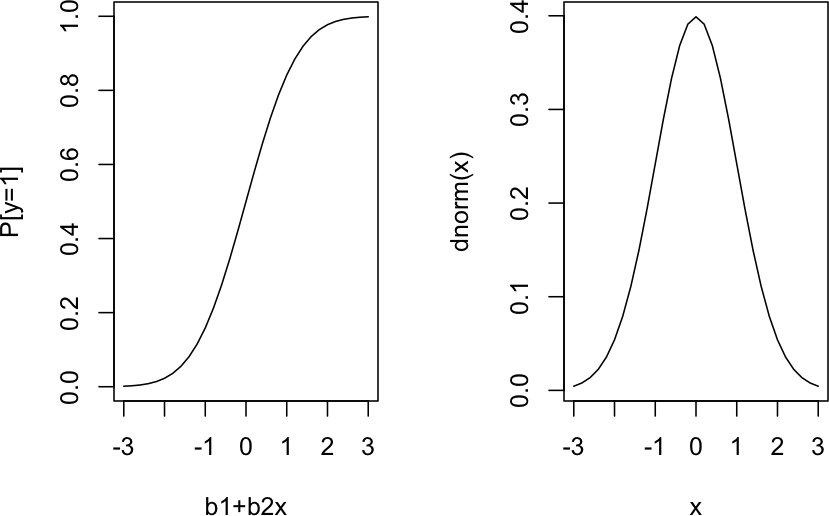
\includegraphics[width=0.8\linewidth]{MEM5220_R_files/figure-latex/fig21-1} 

}

\caption{The shape of the probit function is the standard normal distribution}\label{fig:fig21}
\end{figure}

\begin{Shaded}
\begin{Highlighting}[]
\KeywordTok{detach}\NormalTok{(}\StringTok{"package:PoEdata"}\NormalTok{, }\DataTypeTok{unload=}\OtherTok{TRUE}\NormalTok{)}
\KeywordTok{data}\NormalTok{(}\StringTok{"mroz"}\NormalTok{, }\DataTypeTok{package=}\StringTok{'wooldridge'}\NormalTok{)}
\KeywordTok{attach}\NormalTok{(mroz)}
\end{Highlighting}
\end{Shaded}

\begin{verbatim}
## The following objects are masked from bwght:
## 
##     faminc, fatheduc, motheduc
\end{verbatim}

\begin{verbatim}
## The following object is masked from gpa1:
## 
##     age
\end{verbatim}

\begin{Shaded}
\begin{Highlighting}[]
\CommentTok{# Estimate probit model}
\NormalTok{probitres<-}\KeywordTok{glm}\NormalTok{(inlf}\OperatorTok{~}\NormalTok{nwifeinc}\OperatorTok{+}\NormalTok{educ}\OperatorTok{+}\NormalTok{exper}\OperatorTok{+}\KeywordTok{I}\NormalTok{(exper}\OperatorTok{^}\DecValTok{2}\NormalTok{)}\OperatorTok{+}\NormalTok{age}\OperatorTok{+}\NormalTok{kidslt6}\OperatorTok{+}\NormalTok{kidsge6,}
               \DataTypeTok{family=}\KeywordTok{binomial}\NormalTok{(}\DataTypeTok{link=}\NormalTok{probit),}\DataTypeTok{data=}\NormalTok{mroz)}
\CommentTok{# Summary of results:}
\KeywordTok{summary}\NormalTok{(probitres)}
\end{Highlighting}
\end{Shaded}

\begin{verbatim}
## 
## Call:
## glm(formula = inlf ~ nwifeinc + educ + exper + I(exper^2) + age + 
##     kidslt6 + kidsge6, family = binomial(link = probit), data = mroz)
## 
## Deviance Residuals: 
##     Min       1Q   Median       3Q      Max  
## -2.2156  -0.9151   0.4315   0.8653   2.4553  
## 
## Coefficients:
##               Estimate Std. Error z value Pr(>|z|)    
## (Intercept)  0.2700736  0.5080782   0.532  0.59503    
## nwifeinc    -0.0120236  0.0049392  -2.434  0.01492 *  
## educ         0.1309040  0.0253987   5.154 2.55e-07 ***
## exper        0.1233472  0.0187587   6.575 4.85e-11 ***
## I(exper^2)  -0.0018871  0.0005999  -3.145  0.00166 ** 
## age         -0.0528524  0.0084624  -6.246 4.22e-10 ***
## kidslt6     -0.8683247  0.1183773  -7.335 2.21e-13 ***
## kidsge6      0.0360056  0.0440303   0.818  0.41350    
## ---
## Signif. codes:  0 '***' 0.001 '**' 0.01 '*' 0.05 '.' 0.1 ' ' 1
## 
## (Dispersion parameter for binomial family taken to be 1)
## 
##     Null deviance: 1029.7  on 752  degrees of freedom
## Residual deviance:  802.6  on 745  degrees of freedom
## AIC: 818.6
## 
## Number of Fisher Scoring iterations: 4
\end{verbatim}

\begin{Shaded}
\begin{Highlighting}[]
\CommentTok{# Log likelihood value:}
\KeywordTok{logLik}\NormalTok{(probitres) }
\end{Highlighting}
\end{Shaded}

\begin{verbatim}
## 'log Lik.' -401.3022 (df=8)
\end{verbatim}

\begin{Shaded}
\begin{Highlighting}[]
\CommentTok{# McFadden's pseudo R2:}
\DecValTok{1} \OperatorTok{-}\StringTok{ }\NormalTok{probitres}\OperatorTok{$}\NormalTok{deviance}\OperatorTok{/}\NormalTok{probitres}\OperatorTok{$}\NormalTok{null.deviance}
\end{Highlighting}
\end{Shaded}

\begin{verbatim}
## [1] 0.2205805
\end{verbatim}

Take a boostrap sample for the 95\% confidence interval for each
parameter.

\begin{Shaded}
\begin{Highlighting}[]
\KeywordTok{data}\NormalTok{(}\StringTok{"mroz"}\NormalTok{, }\DataTypeTok{package=}\StringTok{'wooldridge'}\NormalTok{)}

\NormalTok{boot_probitres <-}\StringTok{ }\NormalTok{mroz }\OperatorTok\StringTok{ }
\StringTok{  }\KeywordTok{bootstrap}\NormalTok{(}\DecValTok{500}\NormalTok{) }\OperatorTok\StringTok{ }
\StringTok{  }\KeywordTok{do}\NormalTok{(}\KeywordTok{tidy}\NormalTok{(}\KeywordTok{glm}\NormalTok{(inlf}\OperatorTok{~}\NormalTok{nwifeinc}\OperatorTok{+}\NormalTok{educ}\OperatorTok{+}\NormalTok{exper}\OperatorTok{+}\KeywordTok{I}\NormalTok{(exper}\OperatorTok{^}\DecValTok{2}\NormalTok{)}\OperatorTok{+}\NormalTok{age}\OperatorTok{+}\NormalTok{kidslt6}\OperatorTok{+}\NormalTok{kidsge6,}
               \DataTypeTok{family=}\KeywordTok{binomial}\NormalTok{(}\DataTypeTok{link=}\NormalTok{probit),.)))}
\NormalTok{boot_probitres }\OperatorTok\StringTok{ }
\StringTok{  }\KeywordTok{group_by}\NormalTok{(term) }\OperatorTok\StringTok{ }
\StringTok{  }\NormalTok{dplyr}\OperatorTok{::}\KeywordTok{summarise}\NormalTok{(}\DataTypeTok{low =} \KeywordTok{quantile}\NormalTok{(estimate, }\FloatTok{.025}\NormalTok{), }
                   \DataTypeTok{high =} \KeywordTok{quantile}\NormalTok{(estimate, }\FloatTok{.0975}\NormalTok{))}
\end{Highlighting}
\end{Shaded}

\textbackslash{}begin\{table\}{[}h{]}
\textbackslash{}begin\{raggedright\}

\providecommand{\huxb}[2][0,0,0]{\arrayrulecolor[RGB]{#1}\global\arrayrulewidth=#2pt}
    \providecommand{\huxvb}[2][0,0,0]{\color[RGB]{#1}\vrule width #2pt}
    \providecommand{\huxtpad}[1]{\rule{0pt}{\baselineskip+#1}}
    \providecommand{\huxbpad}[1]{\rule[-#1]{0pt}{#1}}
  \begin{tabularx}{0.566666666666667\textwidth}{p{0.188888888888889\textwidth} p{0.188888888888889\textwidth} p{0.188888888888889\textwidth}}


\par

\textbackslash{}end\{raggedright\} \textbackslash{}end\{table\}

\hypertarget{inference}{%
\subsection{Inference}\label{inference}}

We can implement the test for overall significance for the probit model
using both manual and automatic calculations.

\begin{Shaded}
\begin{Highlighting}[]
\CommentTok{# Test of overall significance:}
\CommentTok{# Manual calculation of the LR test statistic:}
\NormalTok{probitres}\OperatorTok{$}\NormalTok{null.deviance }\OperatorTok{-}\StringTok{ }\NormalTok{probitres}\OperatorTok{$}\NormalTok{deviance}
\end{Highlighting}
\end{Shaded}

\begin{verbatim}
## [1] 227.142
\end{verbatim}

\begin{Shaded}
\begin{Highlighting}[]
\CommentTok{# Automatic calculations including p-values,...:}
\KeywordTok{lrtest}\NormalTok{(probitres)}
\end{Highlighting}
\end{Shaded}

\textbackslash{}begin\{table\}{[}h{]}
\textbackslash{}begin\{raggedright\}

\providecommand{\huxb}[2][0,0,0]{\arrayrulecolor[RGB]{#1}\global\arrayrulewidth=#2pt}
    \providecommand{\huxvb}[2][0,0,0]{\color[RGB]{#1}\vrule width #2pt}
    \providecommand{\huxtpad}[1]{\rule{0pt}{\baselineskip+#1}}
    \providecommand{\huxbpad}[1]{\rule[-#1]{0pt}{#1}}
  \begin{tabularx}{0.622222222222222\textwidth}{p{0.124444444444444\textwidth} p{0.124444444444444\textwidth} p{0.124444444444444\textwidth} p{0.124444444444444\textwidth} p{0.124444444444444\textwidth}}


\par

\textbackslash{}end\{raggedright\} \textbackslash{}end\{table\}

\begin{Shaded}
\begin{Highlighting}[]
\CommentTok{# Test of H0: experience and age are irrelevant}
\NormalTok{restr <-}\StringTok{ }\KeywordTok{glm}\NormalTok{(inlf}\OperatorTok{~}\NormalTok{nwifeinc}\OperatorTok{+}\NormalTok{educ}\OperatorTok{+}\StringTok{ }\NormalTok{kidslt6}\OperatorTok{+}\NormalTok{kidsge6, }
             \DataTypeTok{family=}\KeywordTok{binomial}\NormalTok{(}\DataTypeTok{link=}\NormalTok{logit),}\DataTypeTok{data=}\NormalTok{mroz)}
\KeywordTok{lrtest}\NormalTok{(restr,probitres)}
\end{Highlighting}
\end{Shaded}

\textbackslash{}begin\{table\}{[}h{]}
\textbackslash{}begin\{raggedright\}

\providecommand{\huxb}[2][0,0,0]{\arrayrulecolor[RGB]{#1}\global\arrayrulewidth=#2pt}
    \providecommand{\huxvb}[2][0,0,0]{\color[RGB]{#1}\vrule width #2pt}
    \providecommand{\huxtpad}[1]{\rule{0pt}{\baselineskip+#1}}
    \providecommand{\huxbpad}[1]{\rule[-#1]{0pt}{#1}}
  \begin{tabularx}{0.622222222222222\textwidth}{p{0.124444444444444\textwidth} p{0.124444444444444\textwidth} p{0.124444444444444\textwidth} p{0.124444444444444\textwidth} p{0.124444444444444\textwidth}}


\par

\textbackslash{}end\{raggedright\} \textbackslash{}end\{table\}

\hypertarget{predictions}{%
\subsection{Predictions}\label{predictions}}

The command \texttt{predict()} can calculate predicted values for the
estimation sample or arbitrary sets of regressor values.

We can calculate

\begin{Shaded}
\begin{Highlighting}[]
\CommentTok{# predictions for two "extreme" women:}
\NormalTok{xpred <-}\StringTok{ }\KeywordTok{list}\NormalTok{(}\DataTypeTok{nwifeinc=}\KeywordTok{c}\NormalTok{(}\DecValTok{100}\NormalTok{,}\DecValTok{0}\NormalTok{),}\DataTypeTok{educ=}\KeywordTok{c}\NormalTok{(}\DecValTok{5}\NormalTok{,}\DecValTok{17}\NormalTok{),}\DataTypeTok{exper=}\KeywordTok{c}\NormalTok{(}\DecValTok{0}\NormalTok{,}\DecValTok{30}\NormalTok{),}
              \DataTypeTok{age=}\KeywordTok{c}\NormalTok{(}\DecValTok{20}\NormalTok{,}\DecValTok{52}\NormalTok{),}\DataTypeTok{kidslt6=}\KeywordTok{c}\NormalTok{(}\DecValTok{2}\NormalTok{,}\DecValTok{0}\NormalTok{),}\DataTypeTok{kidsge6=}\KeywordTok{c}\NormalTok{(}\DecValTok{0}\NormalTok{,}\DecValTok{0}\NormalTok{))}
\CommentTok{# Predictions from linear probability, probit and logit model:}
\KeywordTok{predict}\NormalTok{(linprob,  xpred,}\DataTypeTok{type =} \StringTok{"response"}\NormalTok{)}
\end{Highlighting}
\end{Shaded}

\begin{verbatim}
##          1          2 
## -0.4104582  1.0428084
\end{verbatim}

\begin{Shaded}
\begin{Highlighting}[]
\KeywordTok{predict}\NormalTok{(logitres, xpred,}\DataTypeTok{type =} \StringTok{"response"}\NormalTok{)}
\end{Highlighting}
\end{Shaded}

\begin{verbatim}
##           1           2 
## 0.005218002 0.950049117
\end{verbatim}

\begin{Shaded}
\begin{Highlighting}[]
\KeywordTok{predict}\NormalTok{(probitres,xpred,}\DataTypeTok{type =} \StringTok{"response"}\NormalTok{)}
\end{Highlighting}
\end{Shaded}

\begin{verbatim}
##           1           2 
## 0.001065043 0.959869044
\end{verbatim}

\begin{Shaded}
\begin{Highlighting}[]
\CommentTok{# Simulated data}
\KeywordTok{set.seed}\NormalTok{(}\DecValTok{12345}\NormalTok{)}
\NormalTok{y <-}\StringTok{ }\KeywordTok{rbinom}\NormalTok{(}\DecValTok{100}\NormalTok{, }\DecValTok{1}\NormalTok{, }\FloatTok{0.5}\NormalTok{)}
\NormalTok{x <-}\StringTok{ }\KeywordTok{rnorm}\NormalTok{(}\DecValTok{100}\NormalTok{) }\OperatorTok{+}\StringTok{ }\DecValTok{2} \OperatorTok{*}\StringTok{ }\NormalTok{y}

\CommentTok{# Estimation }
\NormalTok{linpr.res <-}\StringTok{ }\KeywordTok{lm}\NormalTok{(y}\OperatorTok{~}\NormalTok{x)}
\NormalTok{logit.res <-}\KeywordTok{glm}\NormalTok{(y }\OperatorTok{~}\NormalTok{x, }\DataTypeTok{family =} \KeywordTok{binomial}\NormalTok{(}\DataTypeTok{link =}\NormalTok{ logit))}
\NormalTok{probit.res <-}\KeywordTok{glm}\NormalTok{(y }\OperatorTok{~}\NormalTok{x, }\DataTypeTok{family =} \KeywordTok{binomial}\NormalTok{(}\DataTypeTok{link =}\NormalTok{ probit))}

\CommentTok{# Prediction from a regular grid of x values}
\NormalTok{xp <-}\StringTok{ }\KeywordTok{seq}\NormalTok{(}\DataTypeTok{from=} \KeywordTok{min}\NormalTok{(x), }\DataTypeTok{to=}\KeywordTok{max}\NormalTok{(x), }\DataTypeTok{length=}\DecValTok{50}\NormalTok{)}
\NormalTok{linpr.p <-}\StringTok{ }\KeywordTok{predict}\NormalTok{(linpr.res, }\KeywordTok{list}\NormalTok{(}\DataTypeTok{x =}\NormalTok{ xp), }\DataTypeTok{type =} \StringTok{"response"}\NormalTok{)}
\NormalTok{logit.p <-}\StringTok{ }\KeywordTok{predict}\NormalTok{(logit.res, }\KeywordTok{list}\NormalTok{(}\DataTypeTok{x =}\NormalTok{ xp), }\DataTypeTok{type =} \StringTok{"response"}\NormalTok{)}
\NormalTok{probit.p <-}\StringTok{ }\KeywordTok{predict}\NormalTok{(probit.res, }\KeywordTok{list}\NormalTok{(}\DataTypeTok{x =}\NormalTok{ xp), }\DataTypeTok{type =} \StringTok{"response"}\NormalTok{)}
\end{Highlighting}
\end{Shaded}

\begin{Shaded}
\begin{Highlighting}[]
\KeywordTok{plot}\NormalTok{(x,y)}
\KeywordTok{lines}\NormalTok{(xp, linpr.p, }\DataTypeTok{lwd=}\DecValTok{2}\NormalTok{, }\DataTypeTok{lty =} \DecValTok{1}\NormalTok{)}
\KeywordTok{lines}\NormalTok{(xp, logit.p, }\DataTypeTok{lwd=}\DecValTok{2}\NormalTok{, }\DataTypeTok{lty =} \DecValTok{2}\NormalTok{)}
\KeywordTok{lines}\NormalTok{(xp, probit.p, }\DataTypeTok{lwd=}\DecValTok{1}\NormalTok{, }\DataTypeTok{lty =} \DecValTok{1}\NormalTok{)}
\KeywordTok{legend}\NormalTok{(}\StringTok{"topleft"}\NormalTok{, }
       \KeywordTok{c}\NormalTok{(}\StringTok{"linear prob."}\NormalTok{, }\StringTok{"logit"}\NormalTok{, }\StringTok{"probit"}\NormalTok{), }
       \DataTypeTok{lwd =} \KeywordTok{c}\NormalTok{(}\DecValTok{2}\NormalTok{,}\DecValTok{2}\NormalTok{,}\DecValTok{1}\NormalTok{), }\DataTypeTok{lty =} \KeywordTok{c}\NormalTok{(}\DecValTok{1}\NormalTok{,}\DecValTok{2}\NormalTok{,}\DecValTok{1}\NormalTok{))}
\end{Highlighting}
\end{Shaded}

\begin{figure}

{\centering 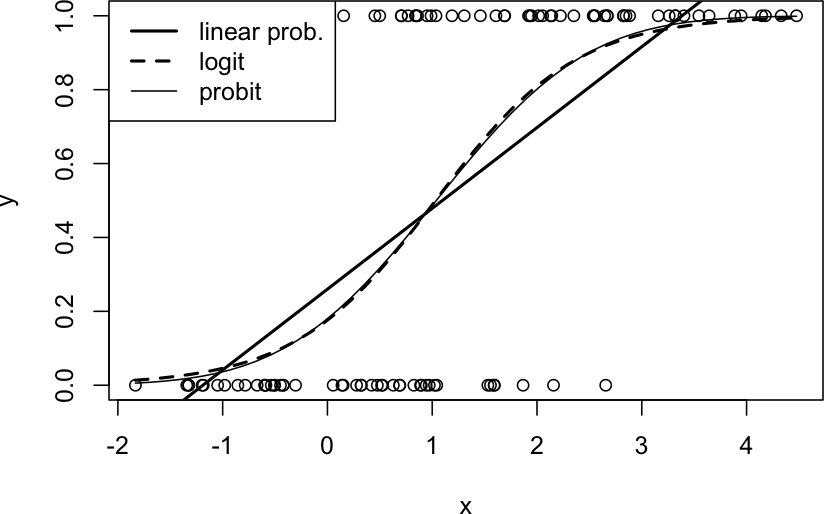
\includegraphics[width=0.8\linewidth]{MEM5220_R_files/figure-latex/fig22-1} 

}

\caption{Predictions from binary response models (simulated data)}\label{fig:fig22}
\end{figure}

\hypertarget{marginal-partial-effects}{%
\subsection{Marginal (partial) effects}\label{marginal-partial-effects}}

Several packages provide estimates of marginal effects for different
types of models. Among these are \textbf{car}, \textbf{alr3},
\textbf{mfx}, \textbf{erer}, among others. Unfortunately, none of these
packages implement marginal effects correctly (i.e., correctly account
for interrelated variables such as interaction terms (e.g., a:b) or
power terms (e.g., I(a\^{}2)) and the packages all implement quite
different interfaces for different types of models. The \textbf{margins}
and \textbf{prediction} packages are a combined effort to calculate
marginal effects that include complex terms and provide a uniform
interface for doing those calculations.

To know how much a variable influences the labour force participation,
one has to use \texttt{margins()} command:

\begin{Shaded}
\begin{Highlighting}[]
\NormalTok{effects_logit_participation <-}\StringTok{ }\KeywordTok{margins}\NormalTok{(logitres) }
\KeywordTok{summary}\NormalTok{(effects_logit_participation)}
\end{Highlighting}
\end{Shaded}

\textbackslash{}begin\{table\}{[}h{]}
\textbackslash{}begin\{raggedright\}

\providecommand{\huxb}[2][0,0,0]{\arrayrulecolor[RGB]{#1}\global\arrayrulewidth=#2pt}
    \providecommand{\huxvb}[2][0,0,0]{\color[RGB]{#1}\vrule width #2pt}
    \providecommand{\huxtpad}[1]{\rule{0pt}{\baselineskip+#1}}
    \providecommand{\huxbpad}[1]{\rule[-#1]{0pt}{#1}}
  \begin{tabularx}{1\textwidth}{p{0.142857142857143\textwidth} p{0.142857142857143\textwidth} p{0.142857142857143\textwidth} p{0.142857142857143\textwidth} p{0.142857142857143\textwidth} p{0.142857142857143\textwidth} p{0.142857142857143\textwidth}}


\par

\textbackslash{}end\{raggedright\} \textbackslash{}end\{table\}

\begin{Shaded}
\begin{Highlighting}[]
\KeywordTok{plot}\NormalTok{(effects_logit_participation)}
\end{Highlighting}
\end{Shaded}

\includegraphics{MEM5220_R_files/figure-latex/unnamed-chunk-168-1.pdf}

If one desires subgroup effects, simply pass a subset of data to the
data argument:

\begin{Shaded}
\begin{Highlighting}[]
\KeywordTok{summary}\NormalTok{(}\KeywordTok{margins}\NormalTok{(logitres, }\DataTypeTok{data =} \KeywordTok{subset}\NormalTok{(mroz, kidslt6 }\OperatorTok{==}\StringTok{ }\DecValTok{0}\NormalTok{))) }\CommentTok{# no kids < 6 years}
\end{Highlighting}
\end{Shaded}

\textbackslash{}begin\{table\}{[}h{]}
\textbackslash{}begin\{raggedright\}

\providecommand{\huxb}[2][0,0,0]{\arrayrulecolor[RGB]{#1}\global\arrayrulewidth=#2pt}
    \providecommand{\huxvb}[2][0,0,0]{\color[RGB]{#1}\vrule width #2pt}
    \providecommand{\huxtpad}[1]{\rule{0pt}{\baselineskip+#1}}
    \providecommand{\huxbpad}[1]{\rule[-#1]{0pt}{#1}}
  \begin{tabularx}{1\textwidth}{p{0.142857142857143\textwidth} p{0.142857142857143\textwidth} p{0.142857142857143\textwidth} p{0.142857142857143\textwidth} p{0.142857142857143\textwidth} p{0.142857142857143\textwidth} p{0.142857142857143\textwidth}}


\par

\textbackslash{}end\{raggedright\} \textbackslash{}end\{table\}

\begin{Shaded}
\begin{Highlighting}[]
\KeywordTok{ggplot}\NormalTok{(}\DataTypeTok{data =} \KeywordTok{summary}\NormalTok{(effects_logit_participation)) }\OperatorTok{+}
\StringTok{  }\KeywordTok{geom_point}\NormalTok{(}\KeywordTok{aes}\NormalTok{(factor, AME)) }\OperatorTok{+}
\StringTok{  }\KeywordTok{geom_errorbar}\NormalTok{(}\KeywordTok{aes}\NormalTok{(}\DataTypeTok{x =}\NormalTok{ factor, }\DataTypeTok{ymin =}\NormalTok{ lower, }\DataTypeTok{ymax =}\NormalTok{ upper)) }\OperatorTok{+}
\StringTok{  }\KeywordTok{geom_hline}\NormalTok{(}\DataTypeTok{yintercept =} \DecValTok{0}\NormalTok{, }\DataTypeTok{color=}\StringTok{"lightgrey"}\NormalTok{) }\OperatorTok{+}
\StringTok{  }\KeywordTok{theme_minimal}\NormalTok{() }\OperatorTok{+}
\StringTok{  }\KeywordTok{theme}\NormalTok{(}\DataTypeTok{axis.text.x =} \KeywordTok{element_text}\NormalTok{(}\DataTypeTok{angle =} \DecValTok{45}\NormalTok{))}
\end{Highlighting}
\end{Shaded}

\begin{figure}

{\centering 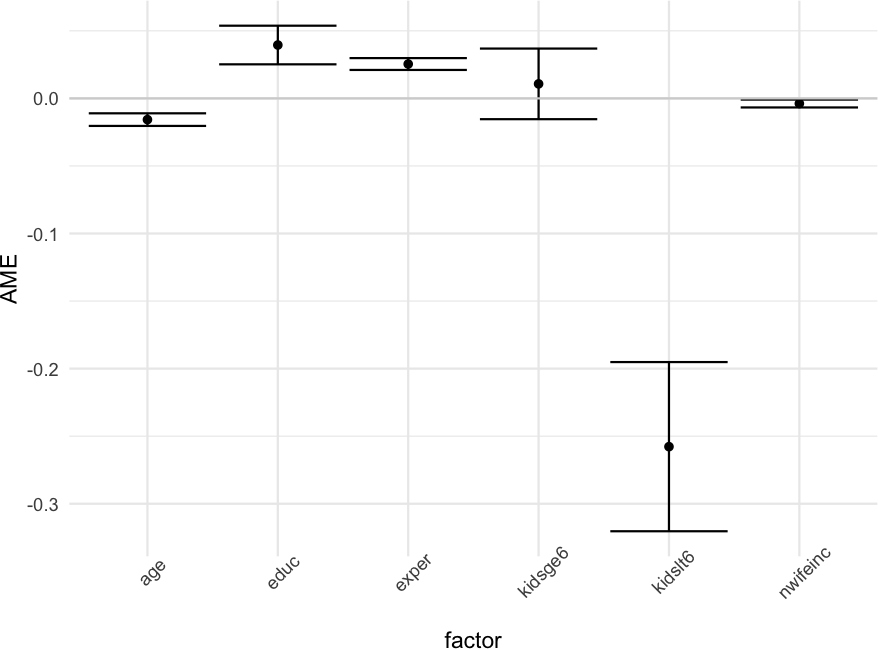
\includegraphics[width=0.8\linewidth]{MEM5220_R_files/figure-latex/fig23-1} 

}

\caption{Logit effect plot}\label{fig:fig23}
\end{figure}

You can also extract the marginal effects of a single variable, with
\texttt{dydx}:

\begin{Shaded}
\begin{Highlighting}[]
\KeywordTok{head}\NormalTok{(}\KeywordTok{dydx}\NormalTok{(mroz, logitres, }\StringTok{"educ"}\NormalTok{))}
\end{Highlighting}
\end{Shaded}

\textbackslash{}begin\{table\}{[}h{]}
\textbackslash{}begin\{raggedright\}

\providecommand{\huxb}[2][0,0,0]{\arrayrulecolor[RGB]{#1}\global\arrayrulewidth=#2pt}
    \providecommand{\huxvb}[2][0,0,0]{\color[RGB]{#1}\vrule width #2pt}
    \providecommand{\huxtpad}[1]{\rule{0pt}{\baselineskip+#1}}
    \providecommand{\huxbpad}[1]{\rule[-#1]{0pt}{#1}}
  \begin{tabularx}{0.2\textwidth}{p{0.2\textwidth}}


\par

\textbackslash{}end\{raggedright\} \textbackslash{}end\{table\}

The function \texttt{cplot()} provides the commonly needed visual
summaries of predictions or average marginal effects conditional on a
covariate.

\begin{Shaded}
\begin{Highlighting}[]
\KeywordTok{cplot}\NormalTok{(logitres, }\DataTypeTok{x =} \StringTok{"educ"}\NormalTok{, }\DataTypeTok{se.type =} \StringTok{"shade"}\NormalTok{)}
\end{Highlighting}
\end{Shaded}

\begin{verbatim}
##    xvals     yvals     upper     lower
## 1    5.0 0.2549509 0.3787666 0.1311353
## 2    5.5 0.2765192 0.3988913 0.1541471
## 3    6.0 0.2991794 0.4190899 0.1792689
## 4    6.5 0.3228678 0.4392936 0.2064421
## 5    7.0 0.3475019 0.4594481 0.2355556
## 6    7.5 0.3729801 0.4795186 0.2664417
## 7    8.0 0.3991836 0.4994946 0.2988726
## 8    8.5 0.4259774 0.5193953 0.3325594
## 9    9.0 0.4532129 0.5392750 0.3671508
## 10   9.5 0.4807315 0.5592299 0.4022331
## 11  10.0 0.5083674 0.5794045 0.4373304
## 12  10.5 0.5359524 0.5999963 0.4719084
## 13  11.0 0.5633190 0.6212490 0.5053891
## 14  11.5 0.5903055 0.6434188 0.5371922
## 15  12.0 0.6167588 0.6666929 0.5668248
## 16  12.5 0.6425384 0.6910722 0.5940047
## 17  13.0 0.6675187 0.7162931 0.6187444
## 18  13.5 0.6915913 0.7418704 0.6413122
## 19  14.0 0.7146659 0.7672368 0.6620950
## 20  14.5 0.7366715 0.7918749 0.6814681
\end{verbatim}

\begin{figure}

{\centering 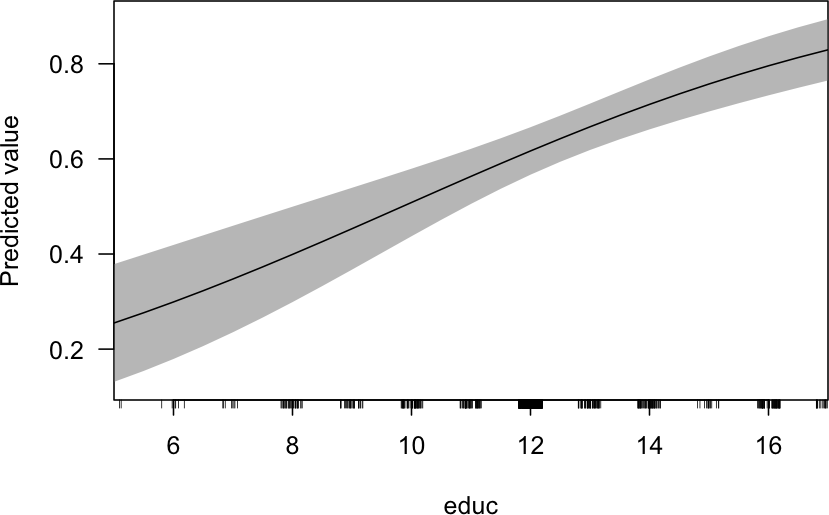
\includegraphics[width=0.8\linewidth]{MEM5220_R_files/figure-latex/fig24-1} 

}

\caption{Marginal effects for logit model}\label{fig:fig24}
\end{figure}

\hypertarget{count-data-the-poisson-regression-model}{%
\section{Count data: The Poisson Regression
Model}\label{count-data-the-poisson-regression-model}}

Instead of just 0/1-coded binary data, count data can take any
non-negative integer \(0, 1, 2, \dots\). If they take very large numbers
(like the number of students in a school), they can be approximated
reasonably well as contiouns variables in a linear models and estimated
using OLS. If the numbers are relativly small, this approximation might
not work well.

The Poisson regression model is the most basic and convenient model
explicitly model explicitly designed for count data.

Poisson regression models can be estimated in R via the \texttt{glm()}
function with the specification \textbf{family= poisson}

Estimating the model with \textbf{quasipoisson} is to adjust for
potential vioalations of the Poisson distribution.

\begin{Shaded}
\begin{Highlighting}[]
\KeywordTok{data}\NormalTok{(crime1, }\DataTypeTok{package=}\StringTok{'wooldridge'}\NormalTok{)}

\CommentTok{# Estimate linear model}
\NormalTok{lm.res      <-}\StringTok{  }\KeywordTok{lm}\NormalTok{(narr86}\OperatorTok{~}\NormalTok{pcnv}\OperatorTok{+}\NormalTok{avgsen}\OperatorTok{+}\NormalTok{tottime}\OperatorTok{+}\NormalTok{ptime86}\OperatorTok{+}\NormalTok{qemp86}\OperatorTok{+}\NormalTok{inc86}\OperatorTok{+}
\StringTok{                     }\NormalTok{black}\OperatorTok{+}\NormalTok{hispan}\OperatorTok{+}\NormalTok{born60, }\DataTypeTok{data=}\NormalTok{crime1)}
\CommentTok{# Estimate Poisson model}
\NormalTok{Poisson.res <-}\StringTok{ }\KeywordTok{glm}\NormalTok{(narr86}\OperatorTok{~}\NormalTok{pcnv}\OperatorTok{+}\NormalTok{avgsen}\OperatorTok{+}\NormalTok{tottime}\OperatorTok{+}\NormalTok{ptime86}\OperatorTok{+}\NormalTok{qemp86}\OperatorTok{+}\NormalTok{inc86}\OperatorTok{+}
\StringTok{                     }\NormalTok{black}\OperatorTok{+}\NormalTok{hispan}\OperatorTok{+}\NormalTok{born60, }\DataTypeTok{data=}\NormalTok{crime1, }\DataTypeTok{family=}\NormalTok{poisson)}
\CommentTok{# Quasi-Poisson model}
\NormalTok{QPoisson.res<-}\StringTok{ }\KeywordTok{glm}\NormalTok{(narr86}\OperatorTok{~}\NormalTok{pcnv}\OperatorTok{+}\NormalTok{avgsen}\OperatorTok{+}\NormalTok{tottime}\OperatorTok{+}\NormalTok{ptime86}\OperatorTok{+}\NormalTok{qemp86}\OperatorTok{+}\NormalTok{inc86}\OperatorTok{+}
\StringTok{                     }\NormalTok{black}\OperatorTok{+}\NormalTok{hispan}\OperatorTok{+}\NormalTok{born60, }\DataTypeTok{data=}\NormalTok{crime1, }\DataTypeTok{family=}\NormalTok{quasipoisson)}
\end{Highlighting}
\end{Shaded}

\begin{Shaded}
\begin{Highlighting}[]
\KeywordTok{stargazer}\NormalTok{(lm.res,Poisson.res,QPoisson.res,}\DataTypeTok{type=}\StringTok{"text"}\NormalTok{,}\DataTypeTok{keep.stat=}\StringTok{"n"}\NormalTok{)}
\end{Highlighting}
\end{Shaded}

\begin{verbatim}
## 
## ==================================================
##                       Dependent variable:         
##              -------------------------------------
##                             narr86                
##                 OLS     Poisson  glm: quasipoisson
##                                     link = log    
##                 (1)       (2)           (3)       
## --------------------------------------------------
## pcnv         -0.132*** -0.402***     -0.402***    
##               (0.040)   (0.085)       (0.105)     
##                                                   
## avgsen        -0.011    -0.024        -0.024      
##               (0.012)   (0.020)       (0.025)     
##                                                   
## tottime        0.012    0.024*         0.024      
##               (0.009)   (0.015)       (0.018)     
##                                                   
## ptime86      -0.041*** -0.099***     -0.099***    
##               (0.009)   (0.021)       (0.025)     
##                                                   
## qemp86       -0.051***  -0.038        -0.038      
##               (0.014)   (0.029)       (0.036)     
##                                                   
## inc86        -0.001*** -0.008***     -0.008***    
##              (0.0003)   (0.001)       (0.001)     
##                                                   
## black        0.327***  0.661***      0.661***     
##               (0.045)   (0.074)       (0.091)     
##                                                   
## hispan       0.194***  0.500***      0.500***     
##               (0.040)   (0.074)       (0.091)     
##                                                   
## born60        -0.022    -0.051        -0.051      
##               (0.033)   (0.064)       (0.079)     
##                                                   
## Constant     0.577***  -0.600***     -0.600***    
##               (0.038)   (0.067)       (0.083)     
##                                                   
## --------------------------------------------------
## Observations   2,725     2,725         2,725      
## ==================================================
## Note:                  *p<0.1; **p<0.05; ***p<0.01
\end{verbatim}

By construction, the parameter estiamtes are the same but the standard
errors are larger for the QMLE.

\hypertarget{corner-solution-response-the-tobit-model}{%
\subsection{Corner Solution Response: The Tobit
Model}\label{corner-solution-response-the-tobit-model}}

Corner solutions describe situations where the variable of interest is
continous but restricted in range. Typically, it cannot be negative.

The package \textbf{censReg} offers the command \texttt{censReg()} for
estimating a Tobit model.

We have already estimated labor supply mdoeld for the women in the
dataset \emph{mroz}, ignoring the fact that the hours worked is
necessarily non-negative.

\begin{Shaded}
\begin{Highlighting}[]
\CommentTok{# Estimate Tobit model using censReg:}
\NormalTok{TobitRes <-}\StringTok{ }\KeywordTok{censReg}\NormalTok{(hours}\OperatorTok{~}\NormalTok{nwifeinc}\OperatorTok{+}\NormalTok{educ}\OperatorTok{+}\NormalTok{exper}\OperatorTok{+}\KeywordTok{I}\NormalTok{(exper}\OperatorTok{^}\DecValTok{2}\NormalTok{)}\OperatorTok{+}\StringTok{ }
\StringTok{                      }\NormalTok{age}\OperatorTok{+}\NormalTok{kidslt6}\OperatorTok{+}\NormalTok{kidsge6, }\DataTypeTok{data=}\NormalTok{mroz )}
\KeywordTok{summary}\NormalTok{(TobitRes)}
\end{Highlighting}
\end{Shaded}

\begin{verbatim}
## 
## Call:
## censReg(formula = hours ~ nwifeinc + educ + exper + I(exper^2) + 
##     age + kidslt6 + kidsge6, data = mroz)
## 
## Observations:
##          Total  Left-censored     Uncensored Right-censored 
##            753            325            428              0 
## 
## Coefficients:
##               Estimate Std. error t value  Pr(> t)    
## (Intercept)  965.30528  446.43613   2.162 0.030599 *  
## nwifeinc      -8.81424    4.45910  -1.977 0.048077 *  
## educ          80.64561   21.58324   3.736 0.000187 ***
## exper        131.56430   17.27939   7.614 2.66e-14 ***
## I(exper^2)    -1.86416    0.53766  -3.467 0.000526 ***
## age          -54.40501    7.41850  -7.334 2.24e-13 ***
## kidslt6     -894.02174  111.87803  -7.991 1.34e-15 ***
## kidsge6      -16.21800   38.64139  -0.420 0.674701    
## logSigma       7.02289    0.03706 189.514  < 2e-16 ***
## ---
## Signif. codes:  0 '***' 0.001 '**' 0.01 '*' 0.05 '.' 0.1 ' ' 1
## 
## Newton-Raphson maximisation, 7 iterations
## Return code 1: gradient close to zero
## Log-likelihood: -3819.095 on 9 Df
\end{verbatim}

\begin{Shaded}
\begin{Highlighting}[]
\CommentTok{# Partial Effects at the average x:}
\KeywordTok{margEff}\NormalTok{(TobitRes)}
\end{Highlighting}
\end{Shaded}

\begin{verbatim}
##    nwifeinc        educ       exper  I(exper^2)         age     kidslt6 
##   -5.326442   48.734094   79.504232   -1.126509  -32.876918 -540.256831 
##     kidsge6 
##   -9.800526
\end{verbatim}

Another alternative for estimating Tobit models is the command
\textbf{survreg} from the package survival. It is less straightforward
to use but more flexible.

\begin{Shaded}
\begin{Highlighting}[]
\CommentTok{# Estimate Tobit model using survreg:}
\NormalTok{res <-}\StringTok{ }\KeywordTok{survreg}\NormalTok{(}\KeywordTok{Surv}\NormalTok{(hours, hours}\OperatorTok{>}\DecValTok{0}\NormalTok{, }\DataTypeTok{type=}\StringTok{"left"}\NormalTok{) }\OperatorTok{~}\StringTok{ }\NormalTok{nwifeinc}\OperatorTok{+}\NormalTok{educ}\OperatorTok{+}\NormalTok{exper}\OperatorTok{+}
\StringTok{                 }\KeywordTok{I}\NormalTok{(exper}\OperatorTok{^}\DecValTok{2}\NormalTok{)}\OperatorTok{+}\NormalTok{age}\OperatorTok{+}\NormalTok{kidslt6}\OperatorTok{+}\NormalTok{kidsge6, }\DataTypeTok{data=}\NormalTok{mroz, }\DataTypeTok{dist=}\StringTok{"gaussian"}\NormalTok{)}
\KeywordTok{summary}\NormalTok{(res)}
\end{Highlighting}
\end{Shaded}

\begin{verbatim}
## 
## Call:
## survreg(formula = Surv(hours, hours > 0, type = "left") ~ nwifeinc + 
##     educ + exper + I(exper^2) + age + kidslt6 + kidsge6, data = mroz, 
##     dist = "gaussian")
##                 Value Std. Error      z       p
## (Intercept)  965.3053   446.4361   2.16 0.03060
## nwifeinc      -8.8142     4.4591  -1.98 0.04808
## educ          80.6456    21.5832   3.74 0.00019
## exper        131.5643    17.2794   7.61 2.7e-14
## I(exper^2)    -1.8642     0.5377  -3.47 0.00053
## age          -54.4050     7.4185  -7.33 2.2e-13
## kidslt6     -894.0217   111.8780  -7.99 1.3e-15
## kidsge6      -16.2180    38.6414  -0.42 0.67470
## Log(scale)     7.0229     0.0371 189.51 < 2e-16
## 
## Scale= 1122 
## 
## Gaussian distribution
## Loglik(model)= -3819.1   Loglik(intercept only)= -3954.9
##  Chisq= 271.59 on 7 degrees of freedom, p= 7e-55 
## Number of Newton-Raphson Iterations: 4 
## n= 753
\end{verbatim}

\hypertarget{censored-and-truncated-regression-models}{%
\section{Censored and Truncated Regression
Models}\label{censored-and-truncated-regression-models}}

Censored regression models are closely related to Tobit models. In the
basic Tobit model we observe \(y = y^*\) in the ``uncensored'' cases
with \(y^* > 0\) and we only know an upper bound for \(y^* \le 0\) if we
observe \$y 0 = \$.

In this example we are are interested in criminal prognosis of
individuals released from prison to reoffend.

\begin{Shaded}
\begin{Highlighting}[]
\KeywordTok{data}\NormalTok{(recid, }\DataTypeTok{package=}\StringTok{'wooldridge'}\NormalTok{)}

\CommentTok{# Define Dummy for UNcensored observations}
\NormalTok{recid}\OperatorTok{$}\NormalTok{uncensored <-}\StringTok{ }\NormalTok{recid}\OperatorTok{$}\NormalTok{cens}\OperatorTok{==}\DecValTok{0}
\CommentTok{# Estimate censored regression model:}
\NormalTok{res<-}\KeywordTok{survreg}\NormalTok{(}\KeywordTok{Surv}\NormalTok{(}\KeywordTok{log}\NormalTok{(durat),uncensored, }\DataTypeTok{type=}\StringTok{"right"}\NormalTok{) }\OperatorTok{~}\StringTok{ }\NormalTok{workprg}\OperatorTok{+}\NormalTok{priors}\OperatorTok{+}
\StringTok{               }\NormalTok{tserved}\OperatorTok{+}\NormalTok{felon}\OperatorTok{+}\NormalTok{alcohol}\OperatorTok{+}\NormalTok{drugs}\OperatorTok{+}\NormalTok{black}\OperatorTok{+}\NormalTok{married}\OperatorTok{+}\NormalTok{educ}\OperatorTok{+}\NormalTok{age, }
             \DataTypeTok{data=}\NormalTok{recid, }\DataTypeTok{dist=}\StringTok{"gaussian"}\NormalTok{)}
\CommentTok{# Output:}
\KeywordTok{summary}\NormalTok{(res)}
\end{Highlighting}
\end{Shaded}

\begin{verbatim}
## 
## Call:
## survreg(formula = Surv(log(durat), uncensored, type = "right") ~ 
##     workprg + priors + tserved + felon + alcohol + drugs + black + 
##         married + educ + age, data = recid, dist = "gaussian")
##                 Value Std. Error     z       p
## (Intercept)  4.099386   0.347535 11.80 < 2e-16
## workprg     -0.062572   0.120037 -0.52  0.6022
## priors      -0.137253   0.021459 -6.40 1.6e-10
## tserved     -0.019331   0.002978 -6.49 8.5e-11
## felon        0.443995   0.145087  3.06  0.0022
## alcohol     -0.634909   0.144217 -4.40 1.1e-05
## drugs       -0.298160   0.132736 -2.25  0.0247
## black       -0.542718   0.117443 -4.62 3.8e-06
## married      0.340684   0.139843  2.44  0.0148
## educ         0.022920   0.025397  0.90  0.3668
## age          0.003910   0.000606  6.45 1.1e-10
## Log(scale)   0.593586   0.034412 17.25 < 2e-16
## 
## Scale= 1.81 
## 
## Gaussian distribution
## Loglik(model)= -1597.1   Loglik(intercept only)= -1680.4
##  Chisq= 166.74 on 10 degrees of freedom, p= 1.3e-30 
## Number of Newton-Raphson Iterations: 4 
## n= 1445
\end{verbatim}

\hypertarget{the-heckman-or-sample-selection-model}{%
\subsection{The Heckman, or Sample Selection
Model}\label{the-heckman-or-sample-selection-model}}

The models are useful when the sample selection is not random, but
whehter an individual is in the sample depends on individual
characteristics. For example, when studying wage determination for
married women, some women are not in the labour force, therefore their
wages are zero.

The Heckit procedure involves two steps, estimating both the selection
equation and the equation of interest. Function \texttt{selection()} in
the \textbf{sampleSelection} package performs both steps; therefore, it
needs both equations among its arguments. (The selection equation is, in
fact, a probit model.)

\begin{Shaded}
\begin{Highlighting}[]
\KeywordTok{data}\NormalTok{(}\StringTok{"mroz"}\NormalTok{, }\DataTypeTok{package=}\StringTok{'wooldridge'}\NormalTok{)}
\NormalTok{wage.heckit <-}\StringTok{ }\KeywordTok{selection}\NormalTok{(inlf}\OperatorTok{~}\NormalTok{age}\OperatorTok{+}\NormalTok{educ}\OperatorTok{+}\KeywordTok{I}\NormalTok{(kidslt6}\OperatorTok{+}\NormalTok{kidsge6)}\OperatorTok{+}\NormalTok{mtr,}
                         \KeywordTok{log}\NormalTok{(wage)}\OperatorTok{~}\NormalTok{educ}\OperatorTok{+}\NormalTok{exper, }
                         \DataTypeTok{data=}\NormalTok{mroz, }\DataTypeTok{method=}\StringTok{"ml"}\NormalTok{)}
\KeywordTok{summary}\NormalTok{(wage.heckit)}
\end{Highlighting}
\end{Shaded}

\begin{verbatim}
## --------------------------------------------
## Tobit 2 model (sample selection model)
## Maximum Likelihood estimation
## Newton-Raphson maximisation, 4 iterations
## Return code 2: successive function values within tolerance limit
## Log-Likelihood: -913.5131 
## 753 observations (325 censored and 428 observed)
## 10 free parameters (df = 743)
## Probit selection equation:
##                      Estimate Std. Error t value Pr(>|t|)    
## (Intercept)           1.53798    0.61889   2.485   0.0132 *  
## age                  -0.01346    0.00603  -2.232   0.0259 *  
## educ                  0.06278    0.02180   2.879   0.0041 ** 
## I(kidslt6 + kidsge6) -0.05108    0.03276  -1.559   0.1194    
## mtr                  -2.20864    0.54620  -4.044 5.81e-05 ***
## Outcome equation:
##             Estimate Std. Error t value Pr(>|t|)    
## (Intercept) 0.646221   0.235569   2.743  0.00623 ** 
## educ        0.066462   0.016573   4.010 6.68e-05 ***
## exper       0.011972   0.004085   2.931  0.00348 ** 
##    Error terms:
##       Estimate Std. Error t value Pr(>|t|)    
## sigma  0.84112    0.04302   19.55   <2e-16 ***
## rho   -0.82768    0.03911  -21.16   <2e-16 ***
## ---
## Signif. codes:  0 '***' 0.001 '**' 0.01 '*' 0.05 '.' 0.1 ' ' 1
## --------------------------------------------
\end{verbatim}

\hypertarget{timeseries}{%
\chapter{Time Series}\label{timeseries}}

To load the dataset and necessary functions:

\begin{Shaded}
\begin{Highlighting}[]
\CommentTok{# This function 1. checks if the packages are installed. 2. It installs the packages if they were not in the list of installed packages. 3. It loads the packages into the workspace}
\CommentTok{# devtools::install_github("ccolonescu/PoEdata")}
\NormalTok{PACKAGES<-}\KeywordTok{c}\NormalTok{(}\StringTok{"PoEdata"}\NormalTok{, }\CommentTok{# R data sets for "Principles of Econometrics" by Hill, Griffiths, an d Lim, 4e, Wiley. https://github.com/ccolonescu/PoEdata}
\StringTok{"wooldridge"}\NormalTok{,  }\CommentTok{# Wooldrige Datasets}
\StringTok{"tidyverse"}\NormalTok{,  }\CommentTok{# for data manipulation and ggplots}
\StringTok{"broom"}\NormalTok{,  }\CommentTok{# Tidy regression output}
\StringTok{"car"}\NormalTok{, }\CommentTok{# Companion to applied regression}
\StringTok{"knitr"}\NormalTok{, }\CommentTok{# knit functions}
\CommentTok{# "kableExtra", # extended knit functions for objects exported from other packages}
\StringTok{"huxtable"}\NormalTok{, }\CommentTok{#  Regression tables, broom compatible}
\StringTok{"stargazer"}\NormalTok{, }\CommentTok{# Regression tables}
\StringTok{"AER"}\NormalTok{, }\CommentTok{#  Functions, data sets, examples, demos, and vignettes for the book Christian Kleiber and Achim Zeileis (2008)}
\StringTok{"MASS"}\NormalTok{,  }\CommentTok{#  Functions and datasets to support Venables and Ripley,  "Modern Applied Statistics with S"}
\StringTok{"eurostat"}\NormalTok{, }\CommentTok{# query data from eurostat}
\StringTok{"stats"}\NormalTok{, }
\StringTok{"fUnitRoots"}\NormalTok{, }\CommentTok{# unit root testing}
\StringTok{"uroot"}\NormalTok{, }
\StringTok{"urca"}\NormalTok{, }\CommentTok{# unit root testing}
\StringTok{"forecast"}\NormalTok{, }\CommentTok{# forecast functions}
\StringTok{"astsa"}\NormalTok{, }\CommentTok{# applied statistcal time series analysis }
\StringTok{"modelr"}\NormalTok{, }\CommentTok{# model simulation/ boostraping the modern way}
\StringTok{"magrittr"}\NormalTok{) }\CommentTok{#  pipes}
\NormalTok{inst<-}\KeywordTok{match}\NormalTok{(PACKAGES, }\KeywordTok{.packages}\NormalTok{(}\DataTypeTok{all=}\OtherTok{TRUE}\NormalTok{))}
\NormalTok{need<-}\KeywordTok{which}\NormalTok{(}\KeywordTok{is.na}\NormalTok{(inst))}
\ControlFlowTok{if}\NormalTok{ (}\KeywordTok{length}\NormalTok{(need)}\OperatorTok{>}\DecValTok{0}\NormalTok{) }\KeywordTok{install.packages}\NormalTok{(PACKAGES[need])}
\KeywordTok{lapply}\NormalTok{(PACKAGES, require, }\DataTypeTok{character.only=}\NormalTok{T)}
\end{Highlighting}
\end{Shaded}

In this tutorial we discuss various time series objects in R. We will
cover objects time series, zoo and xts. Base R has limited functionality
for handling time series data. There are several R packages with
functions for creating, manipulating and visualizing time date and time
series objects. The packages that we will use are \texttt{lubridate},
\texttt{quantmod}, \texttt{timeDate}, \texttt{timeSeries}, \texttt{zoo},
\texttt{xts}, \texttt{xtsExtra}, \texttt{tsibble}.

We download monthly CPI from Eurostat

\begin{Shaded}
\begin{Highlighting}[]
\CommentTok{#Since 1996}
\NormalTok{cpi<-}\StringTok{ }\KeywordTok{get_eurostat}\NormalTok{(}\StringTok{"prc_hicp_midx"}\NormalTok{, }\DataTypeTok{filters =} \KeywordTok{list}\NormalTok{(}\DataTypeTok{geo =} \StringTok{"EE"}\NormalTok{, }\DataTypeTok{coicop=}\StringTok{"CP00"}\NormalTok{, }\DataTypeTok{unit=}\StringTok{"I15"}\NormalTok{)) }\OperatorTok
\StringTok{  }\NormalTok{dplyr}\OperatorTok{::}\KeywordTok{filter}\NormalTok{(time}\OperatorTok{>=}\KeywordTok{as.Date}\NormalTok{(}\StringTok{"1992-01-01"}\NormalTok{)) }\OperatorTok\StringTok{  }\NormalTok{dplyr}\OperatorTok{::}\KeywordTok{select}\NormalTok{(time, values) }\OperatorTok\StringTok{ }
\StringTok{  }\KeywordTok{rename}\NormalTok{(}\DataTypeTok{cpi=}\NormalTok{values, }\DataTypeTok{Date=}\NormalTok{time)}
\KeywordTok{plot}\NormalTok{(cpi, }\DataTypeTok{type=}\StringTok{"l"}\NormalTok{)}
\end{Highlighting}
\end{Shaded}

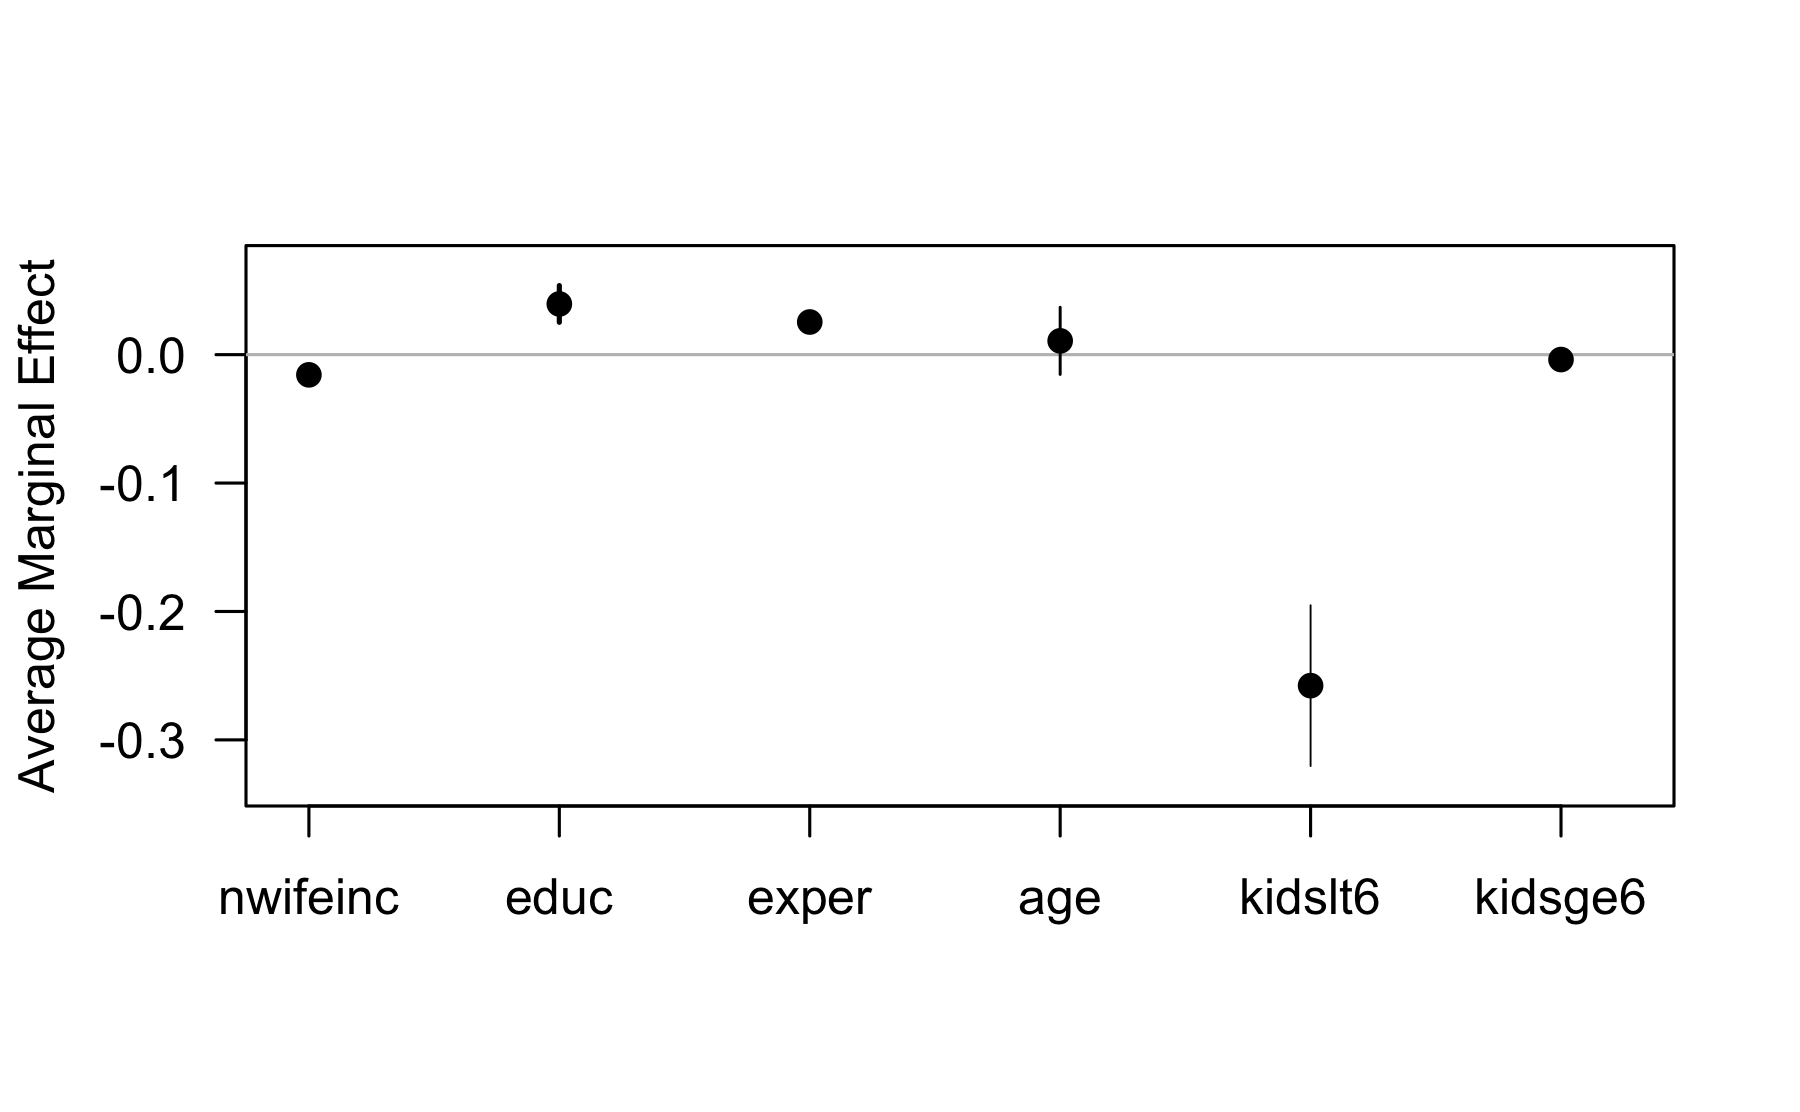
\includegraphics{MEM5220_R_files/figure-latex/unnamed-chunk-178-1.pdf}

The \texttt{data.frame} object is not designed to work efficiently with
time series data. The default plotting methods in R are not designed for
handling time series data. Depending on your data set and the purpose of
your analysis you may need more flexible objects.

\begin{longtable}[]{@{}lll@{}}
\toprule
\begin{minipage}[b]{0.12\columnwidth}\raggedright
object\strut
\end{minipage} & \begin{minipage}[b]{0.15\columnwidth}\raggedright
package\strut
\end{minipage} & \begin{minipage}[b]{0.64\columnwidth}\raggedright
explanation\strut
\end{minipage}\tabularnewline
\midrule
\endhead
\begin{minipage}[t]{0.12\columnwidth}\raggedright
fts\strut
\end{minipage} & \begin{minipage}[t]{0.15\columnwidth}\raggedright
from package fts\strut
\end{minipage} & \begin{minipage}[t]{0.64\columnwidth}\raggedright
An R interfact to tslib (a time series library in C++)\strut
\end{minipage}\tabularnewline
\begin{minipage}[t]{0.12\columnwidth}\raggedright
its\strut
\end{minipage} & \begin{minipage}[t]{0.15\columnwidth}\raggedright
its\strut
\end{minipage} & \begin{minipage}[t]{0.64\columnwidth}\raggedright
for handling irregular time series\strut
\end{minipage}\tabularnewline
\begin{minipage}[t]{0.12\columnwidth}\raggedright
irts\strut
\end{minipage} & \begin{minipage}[t]{0.15\columnwidth}\raggedright
tseries\strut
\end{minipage} & \begin{minipage}[t]{0.64\columnwidth}\raggedright
irregular time‐series objects\strut
\end{minipage}\tabularnewline
\begin{minipage}[t]{0.12\columnwidth}\raggedright
timeSeries\strut
\end{minipage} & \begin{minipage}[t]{0.15\columnwidth}\raggedright
timeSeries\strut
\end{minipage} & \begin{minipage}[t]{0.64\columnwidth}\raggedright
Rmetrics package of time series tools and utilities\strut
\end{minipage}\tabularnewline
\begin{minipage}[t]{0.12\columnwidth}\raggedright
ti\strut
\end{minipage} & \begin{minipage}[t]{0.15\columnwidth}\raggedright
tis\strut
\end{minipage} & \begin{minipage}[t]{0.64\columnwidth}\raggedright
Functions for time indexes and time indexed series\strut
\end{minipage}\tabularnewline
\begin{minipage}[t]{0.12\columnwidth}\raggedright
ts, mts\strut
\end{minipage} & \begin{minipage}[t]{0.15\columnwidth}\raggedright
stats\strut
\end{minipage} & \begin{minipage}[t]{0.64\columnwidth}\raggedright
Regularly spaced time series objects\strut
\end{minipage}\tabularnewline
\begin{minipage}[t]{0.12\columnwidth}\raggedright
zoo\strut
\end{minipage} & \begin{minipage}[t]{0.15\columnwidth}\raggedright
zoo\strut
\end{minipage} & \begin{minipage}[t]{0.64\columnwidth}\raggedright
indexed totally ordered observations which includes irregular time
series\strut
\end{minipage}\tabularnewline
\begin{minipage}[t]{0.12\columnwidth}\raggedright
xts\strut
\end{minipage} & \begin{minipage}[t]{0.15\columnwidth}\raggedright
xts\strut
\end{minipage} & \begin{minipage}[t]{0.64\columnwidth}\raggedright
Extension of the zoo class\strut
\end{minipage}\tabularnewline
\bottomrule
\end{longtable}

For simple regularly spaced time series (e.g monthly, quarterly and
yearly data), you may use \texttt{ts} object from \texttt{stats}
package. For irregular time series data (e.g.~daily data with gaps), you
may prefer \texttt{zoo} or \texttt{irts}object if date is important for
you. If the date does not matter, then simple time series object
\texttt{ts}should be enough.

\begin{Shaded}
\begin{Highlighting}[]
\KeywordTok{head}\NormalTok{(cpi)}
\end{Highlighting}
\end{Shaded}

\textbackslash{}begin\{table\}{[}h{]}
\textbackslash{}begin\{raggedright\}

\providecommand{\huxb}[2][0,0,0]{\arrayrulecolor[RGB]{#1}\global\arrayrulewidth=#2pt}
    \providecommand{\huxvb}[2][0,0,0]{\color[RGB]{#1}\vrule width #2pt}
    \providecommand{\huxtpad}[1]{\rule{0pt}{\baselineskip+#1}}
    \providecommand{\huxbpad}[1]{\rule[-#1]{0pt}{#1}}
  \begin{tabularx}{0.2\textwidth}{p{0.1\textwidth} p{0.1\textwidth}}


\par

\textbackslash{}end\{raggedright\} \textbackslash{}end\{table\}

\begin{Shaded}
\begin{Highlighting}[]
\NormalTok{cpits <-}\StringTok{  }\KeywordTok{ts}\NormalTok{(cpi}\OperatorTok{$}\NormalTok{cpi, }\DataTypeTok{start=}\KeywordTok{c}\NormalTok{(}\DecValTok{1996}\NormalTok{,}\DecValTok{1}\NormalTok{), }\DataTypeTok{frequency =} \DecValTok{12}\NormalTok{)}
\CommentTok{#check structure}
\KeywordTok{str}\NormalTok{(cpits)}
\end{Highlighting}
\end{Shaded}

\begin{verbatim}
##  Time-Series [1:273] from 1996 to 2019: 42.9 44.2 45 45.7 46 ...
\end{verbatim}

\begin{Shaded}
\begin{Highlighting}[]
\KeywordTok{plot}\NormalTok{(cpits)}
\end{Highlighting}
\end{Shaded}

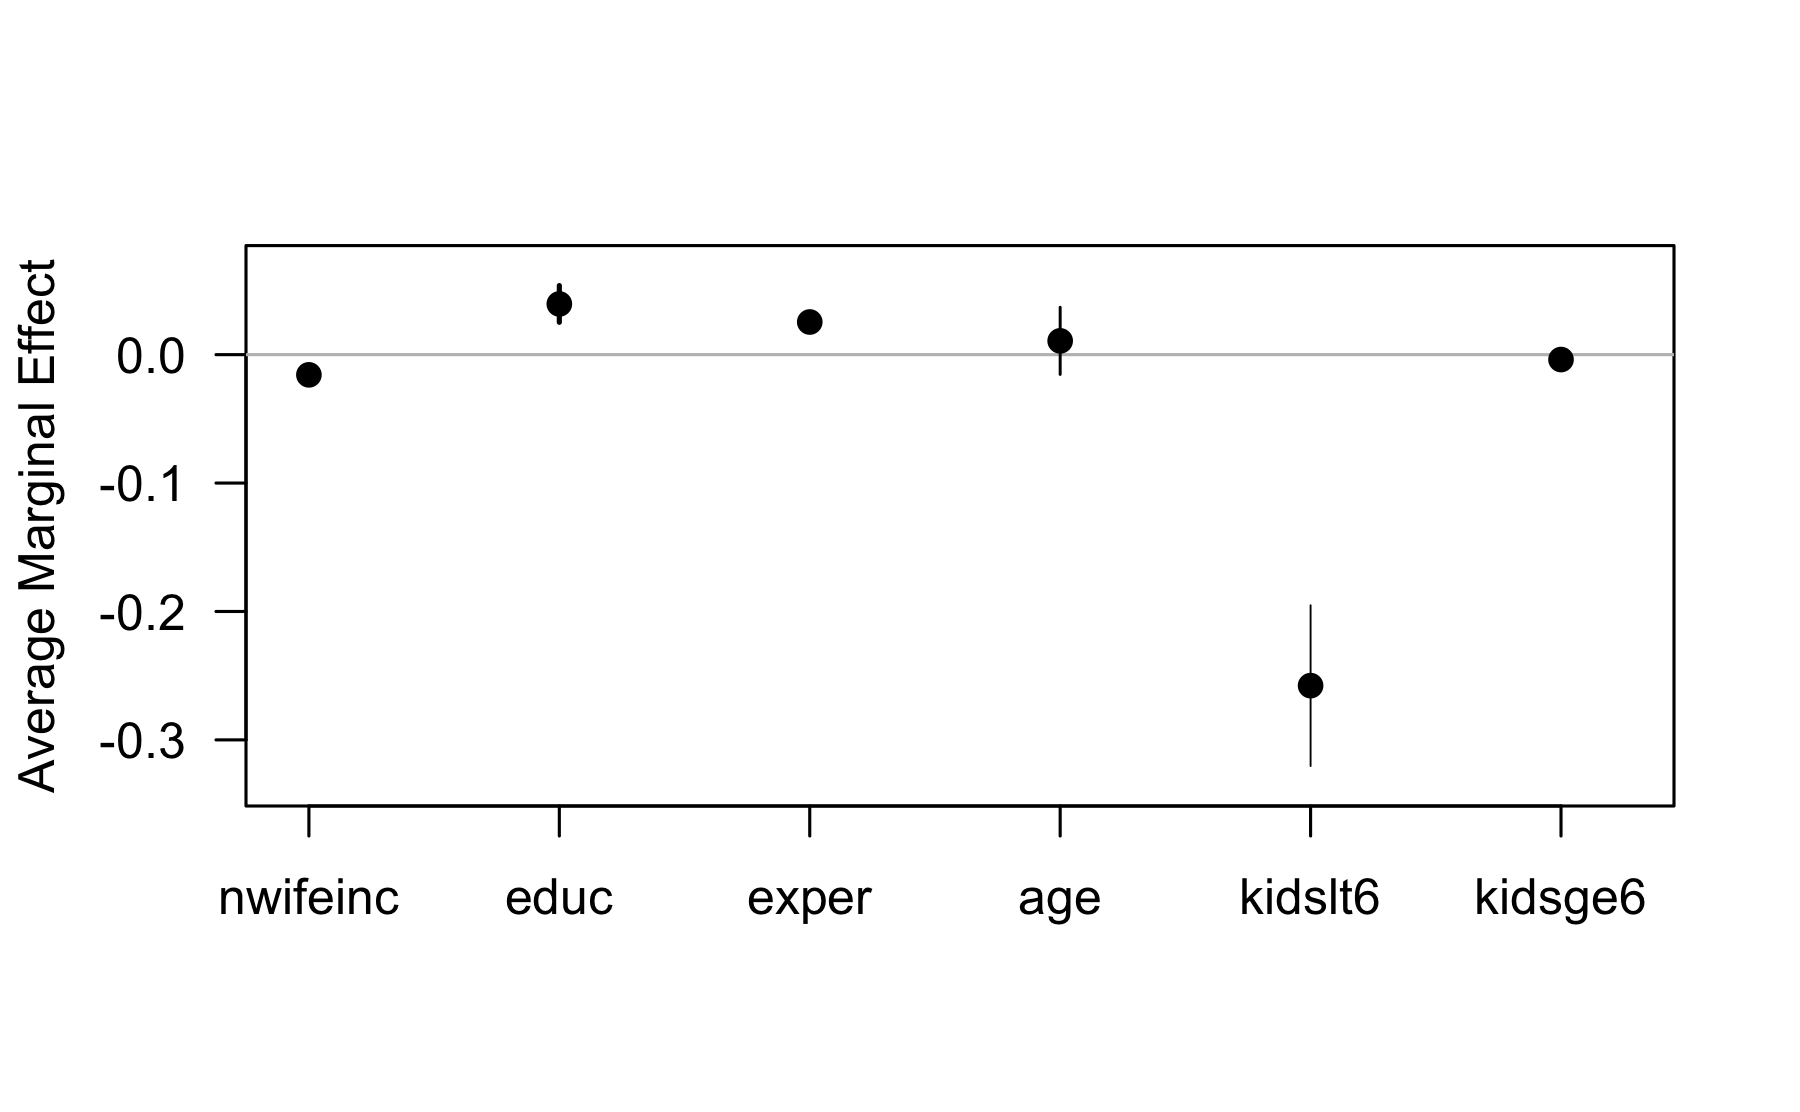
\includegraphics{MEM5220_R_files/figure-latex/unnamed-chunk-179-1.pdf}

\begin{Shaded}
\begin{Highlighting}[]
\CommentTok{#Some functions to characterise time series}
\CommentTok{#Position in the cycle}
\KeywordTok{cycle}\NormalTok{(cpits)}
\end{Highlighting}
\end{Shaded}

\begin{verbatim}
##      Jan Feb Mar Apr May Jun Jul Aug Sep Oct Nov Dec
## 1996   1   2   3   4   5   6   7   8   9  10  11  12
## 1997   1   2   3   4   5   6   7   8   9  10  11  12
## 1998   1   2   3   4   5   6   7   8   9  10  11  12
## 1999   1   2   3   4   5   6   7   8   9  10  11  12
## 2000   1   2   3   4   5   6   7   8   9  10  11  12
## 2001   1   2   3   4   5   6   7   8   9  10  11  12
## 2002   1   2   3   4   5   6   7   8   9  10  11  12
## 2003   1   2   3   4   5   6   7   8   9  10  11  12
## 2004   1   2   3   4   5   6   7   8   9  10  11  12
## 2005   1   2   3   4   5   6   7   8   9  10  11  12
## 2006   1   2   3   4   5   6   7   8   9  10  11  12
## 2007   1   2   3   4   5   6   7   8   9  10  11  12
## 2008   1   2   3   4   5   6   7   8   9  10  11  12
## 2009   1   2   3   4   5   6   7   8   9  10  11  12
## 2010   1   2   3   4   5   6   7   8   9  10  11  12
## 2011   1   2   3   4   5   6   7   8   9  10  11  12
## 2012   1   2   3   4   5   6   7   8   9  10  11  12
## 2013   1   2   3   4   5   6   7   8   9  10  11  12
## 2014   1   2   3   4   5   6   7   8   9  10  11  12
## 2015   1   2   3   4   5   6   7   8   9  10  11  12
## 2016   1   2   3   4   5   6   7   8   9  10  11  12
## 2017   1   2   3   4   5   6   7   8   9  10  11  12
## 2018   1   2   3   4   5   6   7   8   9
\end{verbatim}

\begin{Shaded}
\begin{Highlighting}[]
\CommentTok{#to check frequency}
\KeywordTok{frequency}\NormalTok{(cpits)}
\end{Highlighting}
\end{Shaded}

\begin{verbatim}
## [1] 12
\end{verbatim}

\begin{Shaded}
\begin{Highlighting}[]
\CommentTok{#How time is represented? As a fraction of the year!}
\KeywordTok{time}\NormalTok{(cpits)}
\end{Highlighting}
\end{Shaded}

\begin{verbatim}
##           Jan      Feb      Mar      Apr      May      Jun      Jul
## 1996 1996.000 1996.083 1996.167 1996.250 1996.333 1996.417 1996.500
## 1997 1997.000 1997.083 1997.167 1997.250 1997.333 1997.417 1997.500
## 1998 1998.000 1998.083 1998.167 1998.250 1998.333 1998.417 1998.500
## 1999 1999.000 1999.083 1999.167 1999.250 1999.333 1999.417 1999.500
## 2000 2000.000 2000.083 2000.167 2000.250 2000.333 2000.417 2000.500
## 2001 2001.000 2001.083 2001.167 2001.250 2001.333 2001.417 2001.500
## 2002 2002.000 2002.083 2002.167 2002.250 2002.333 2002.417 2002.500
## 2003 2003.000 2003.083 2003.167 2003.250 2003.333 2003.417 2003.500
## 2004 2004.000 2004.083 2004.167 2004.250 2004.333 2004.417 2004.500
## 2005 2005.000 2005.083 2005.167 2005.250 2005.333 2005.417 2005.500
## 2006 2006.000 2006.083 2006.167 2006.250 2006.333 2006.417 2006.500
## 2007 2007.000 2007.083 2007.167 2007.250 2007.333 2007.417 2007.500
## 2008 2008.000 2008.083 2008.167 2008.250 2008.333 2008.417 2008.500
## 2009 2009.000 2009.083 2009.167 2009.250 2009.333 2009.417 2009.500
## 2010 2010.000 2010.083 2010.167 2010.250 2010.333 2010.417 2010.500
## 2011 2011.000 2011.083 2011.167 2011.250 2011.333 2011.417 2011.500
## 2012 2012.000 2012.083 2012.167 2012.250 2012.333 2012.417 2012.500
## 2013 2013.000 2013.083 2013.167 2013.250 2013.333 2013.417 2013.500
## 2014 2014.000 2014.083 2014.167 2014.250 2014.333 2014.417 2014.500
## 2015 2015.000 2015.083 2015.167 2015.250 2015.333 2015.417 2015.500
## 2016 2016.000 2016.083 2016.167 2016.250 2016.333 2016.417 2016.500
## 2017 2017.000 2017.083 2017.167 2017.250 2017.333 2017.417 2017.500
## 2018 2018.000 2018.083 2018.167 2018.250 2018.333 2018.417 2018.500
##           Aug      Sep      Oct      Nov      Dec
## 1996 1996.583 1996.667 1996.750 1996.833 1996.917
## 1997 1997.583 1997.667 1997.750 1997.833 1997.917
## 1998 1998.583 1998.667 1998.750 1998.833 1998.917
## 1999 1999.583 1999.667 1999.750 1999.833 1999.917
## 2000 2000.583 2000.667 2000.750 2000.833 2000.917
## 2001 2001.583 2001.667 2001.750 2001.833 2001.917
## 2002 2002.583 2002.667 2002.750 2002.833 2002.917
## 2003 2003.583 2003.667 2003.750 2003.833 2003.917
## 2004 2004.583 2004.667 2004.750 2004.833 2004.917
## 2005 2005.583 2005.667 2005.750 2005.833 2005.917
## 2006 2006.583 2006.667 2006.750 2006.833 2006.917
## 2007 2007.583 2007.667 2007.750 2007.833 2007.917
## 2008 2008.583 2008.667 2008.750 2008.833 2008.917
## 2009 2009.583 2009.667 2009.750 2009.833 2009.917
## 2010 2010.583 2010.667 2010.750 2010.833 2010.917
## 2011 2011.583 2011.667 2011.750 2011.833 2011.917
## 2012 2012.583 2012.667 2012.750 2012.833 2012.917
## 2013 2013.583 2013.667 2013.750 2013.833 2013.917
## 2014 2014.583 2014.667 2014.750 2014.833 2014.917
## 2015 2015.583 2015.667 2015.750 2015.833 2015.917
## 2016 2016.583 2016.667 2016.750 2016.833 2016.917
## 2017 2017.583 2017.667 2017.750 2017.833 2017.917
## 2018 2018.583 2018.667
\end{verbatim}

\begin{Shaded}
\begin{Highlighting}[]
\CommentTok{#average difference between time units (0.08333 years or =1/12)}
\KeywordTok{deltat}\NormalTok{(cpits)}
\end{Highlighting}
\end{Shaded}

\begin{verbatim}
## [1] 0.08333333
\end{verbatim}

\hypertarget{seasonal-decomposition-of-time-series}{%
\section{Seasonal decomposition of time
Series}\label{seasonal-decomposition-of-time-series}}

We use \texttt{stl} from package \texttt{stats} to decompose time
series. See the options of the command for details. In addition, we
apply the command \texttt{acf2} from package \texttt{astsa} to
illustrate how we can use the components.

\begin{Shaded}
\begin{Highlighting}[]
\CommentTok{#Fixed seasonal components, s.window - seasonal window}
\KeywordTok{plot}\NormalTok{(}\KeywordTok{stl}\NormalTok{(cpits, }\DataTypeTok{s.window=}\StringTok{"periodic"}\NormalTok{))}
\end{Highlighting}
\end{Shaded}

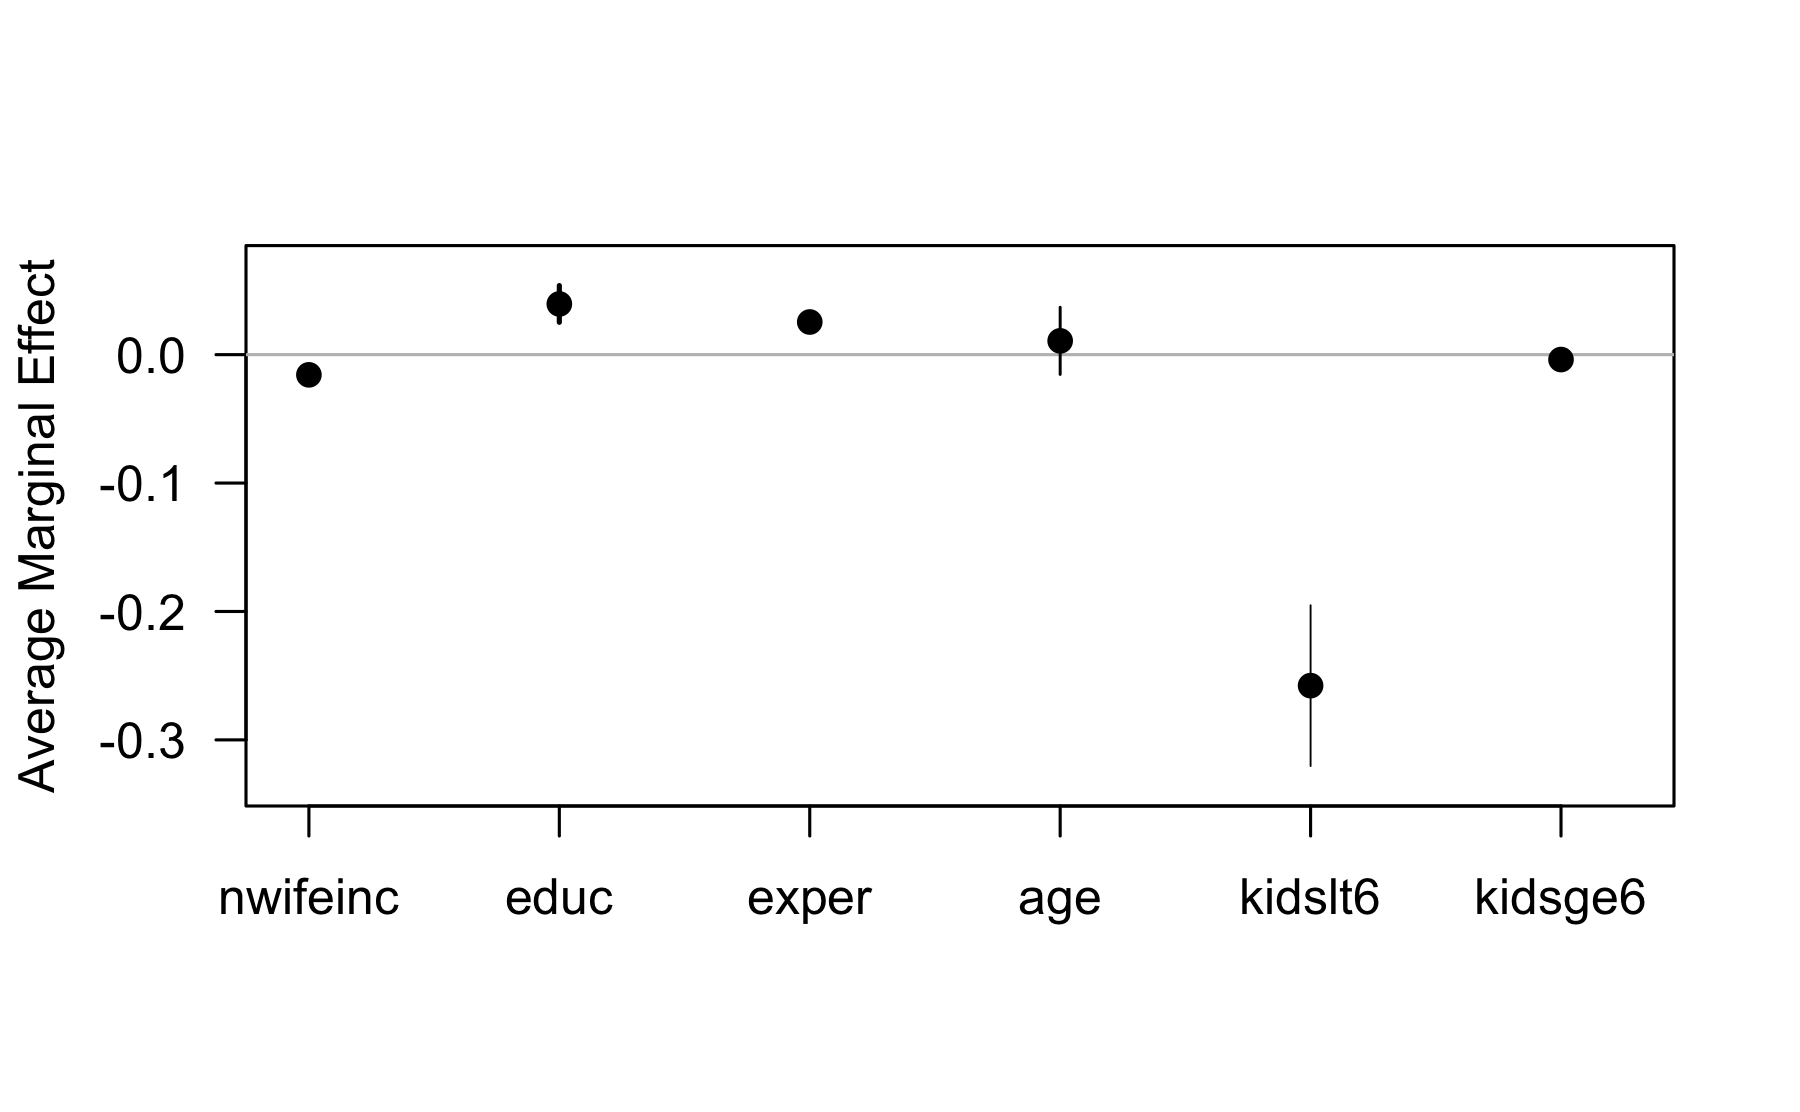
\includegraphics{MEM5220_R_files/figure-latex/unnamed-chunk-180-1.pdf}

\begin{Shaded}
\begin{Highlighting}[]
\CommentTok{#vertical bars on the right reflect the scale of the components}

\CommentTok{#smoothed seasonal component}
\KeywordTok{plot}\NormalTok{(}\KeywordTok{stl}\NormalTok{(cpits, }\DataTypeTok{s.window=}\DecValTok{7}\NormalTok{))}
\end{Highlighting}
\end{Shaded}

\includegraphics{MEM5220_R_files/figure-latex/unnamed-chunk-180-2.pdf}

\begin{Shaded}
\begin{Highlighting}[]
\CommentTok{#remainder component seem to follow AR process}
\CommentTok{#We can make the stl components as object and analyse these separately}
\NormalTok{cpicomponents <-}\StringTok{ }\KeywordTok{stl}\NormalTok{(cpits, }\DataTypeTok{s.window=}\DecValTok{7}\NormalTok{)}

\CommentTok{#remainder}
\KeywordTok{plot}\NormalTok{(cpicomponents}\OperatorTok{$}\NormalTok{time.series[,}\DecValTok{3}\NormalTok{])}
\end{Highlighting}
\end{Shaded}

\includegraphics{MEM5220_R_files/figure-latex/unnamed-chunk-180-3.pdf}

\begin{Shaded}
\begin{Highlighting}[]
\CommentTok{#Autocorrelation function of the remainder}
\KeywordTok{acf2}\NormalTok{(cpicomponents}\OperatorTok{$}\NormalTok{time.series[,}\DecValTok{3}\NormalTok{])}
\end{Highlighting}
\end{Shaded}

\includegraphics{MEM5220_R_files/figure-latex/unnamed-chunk-180-4.pdf}

\begin{verbatim}
##         ACF  PACF
##  [1,]  0.75  0.75
##  [2,]  0.51 -0.12
##  [3,]  0.32 -0.03
##  [4,]  0.21  0.01
##  [5,]  0.15  0.04
##  [6,]  0.13  0.04
##  [7,]  0.12  0.02
##  [8,]  0.06 -0.11
##  [9,]  0.02  0.01
## [10,] -0.06 -0.11
## [11,] -0.22 -0.28
## [12,] -0.43 -0.31
## [13,] -0.43  0.21
## [14,] -0.39 -0.07
## [15,] -0.33 -0.06
## [16,] -0.25  0.08
## [17,] -0.20 -0.02
## [18,] -0.17  0.01
## [19,] -0.18 -0.01
## [20,] -0.14  0.03
## [21,] -0.10  0.07
## [22,] -0.13 -0.21
## [23,] -0.12 -0.11
## [24,] -0.09 -0.15
## [25,] -0.03  0.12
## [26,]  0.05  0.03
## [27,]  0.10 -0.07
## [28,]  0.09 -0.02
## [29,]  0.05 -0.03
## [30,]  0.02 -0.04
## [31,]  0.02  0.01
## [32,]  0.01 -0.01
## [33,]  0.00  0.06
## [34,]  0.01 -0.15
## [35,]  0.04 -0.01
## [36,]  0.05 -0.12
## [37,]  0.08  0.14
## [38,]  0.06  0.00
## [39,]  0.02 -0.06
## [40,] -0.02 -0.03
## [41,] -0.01  0.01
## [42,]  0.02 -0.01
## [43,]  0.03  0.03
## [44,]  0.03 -0.09
## [45,]  0.00  0.02
## [46,]  0.01 -0.04
## [47,] -0.02 -0.15
## [48,] -0.03 -0.07
\end{verbatim}

\hypertarget{differences-and-lags}{%
\section{Differences and lags}\label{differences-and-lags}}

We can apply standard functions to time series, such as differences,
seasonal differences, logs, etc. Let's use CPI to calculate monthly and
annual inflation rates.

\begin{Shaded}
\begin{Highlighting}[]
\KeywordTok{head}\NormalTok{(cpi)}
\end{Highlighting}
\end{Shaded}

\textbackslash{}begin\{table\}{[}h{]}
\textbackslash{}begin\{raggedright\}

\providecommand{\huxb}[2][0,0,0]{\arrayrulecolor[RGB]{#1}\global\arrayrulewidth=#2pt}
    \providecommand{\huxvb}[2][0,0,0]{\color[RGB]{#1}\vrule width #2pt}
    \providecommand{\huxtpad}[1]{\rule{0pt}{\baselineskip+#1}}
    \providecommand{\huxbpad}[1]{\rule[-#1]{0pt}{#1}}
  \begin{tabularx}{0.2\textwidth}{p{0.1\textwidth} p{0.1\textwidth}}


\par

\textbackslash{}end\{raggedright\} \textbackslash{}end\{table\}

\begin{Shaded}
\begin{Highlighting}[]
\NormalTok{cpits <-}\StringTok{  }\KeywordTok{ts}\NormalTok{(cpi}\OperatorTok{$}\NormalTok{cpi, }\DataTypeTok{start=}\KeywordTok{c}\NormalTok{(}\DecValTok{1996}\NormalTok{,}\DecValTok{1}\NormalTok{), }\DataTypeTok{frequency =} \DecValTok{12}\NormalTok{)}
\CommentTok{#check structure}
\KeywordTok{str}\NormalTok{(cpits)}
\end{Highlighting}
\end{Shaded}

\begin{verbatim}
##  Time-Series [1:273] from 1996 to 2019: 42.9 44.2 45 45.7 46 ...
\end{verbatim}

\begin{Shaded}
\begin{Highlighting}[]
\KeywordTok{plot}\NormalTok{(cpits)}
\end{Highlighting}
\end{Shaded}

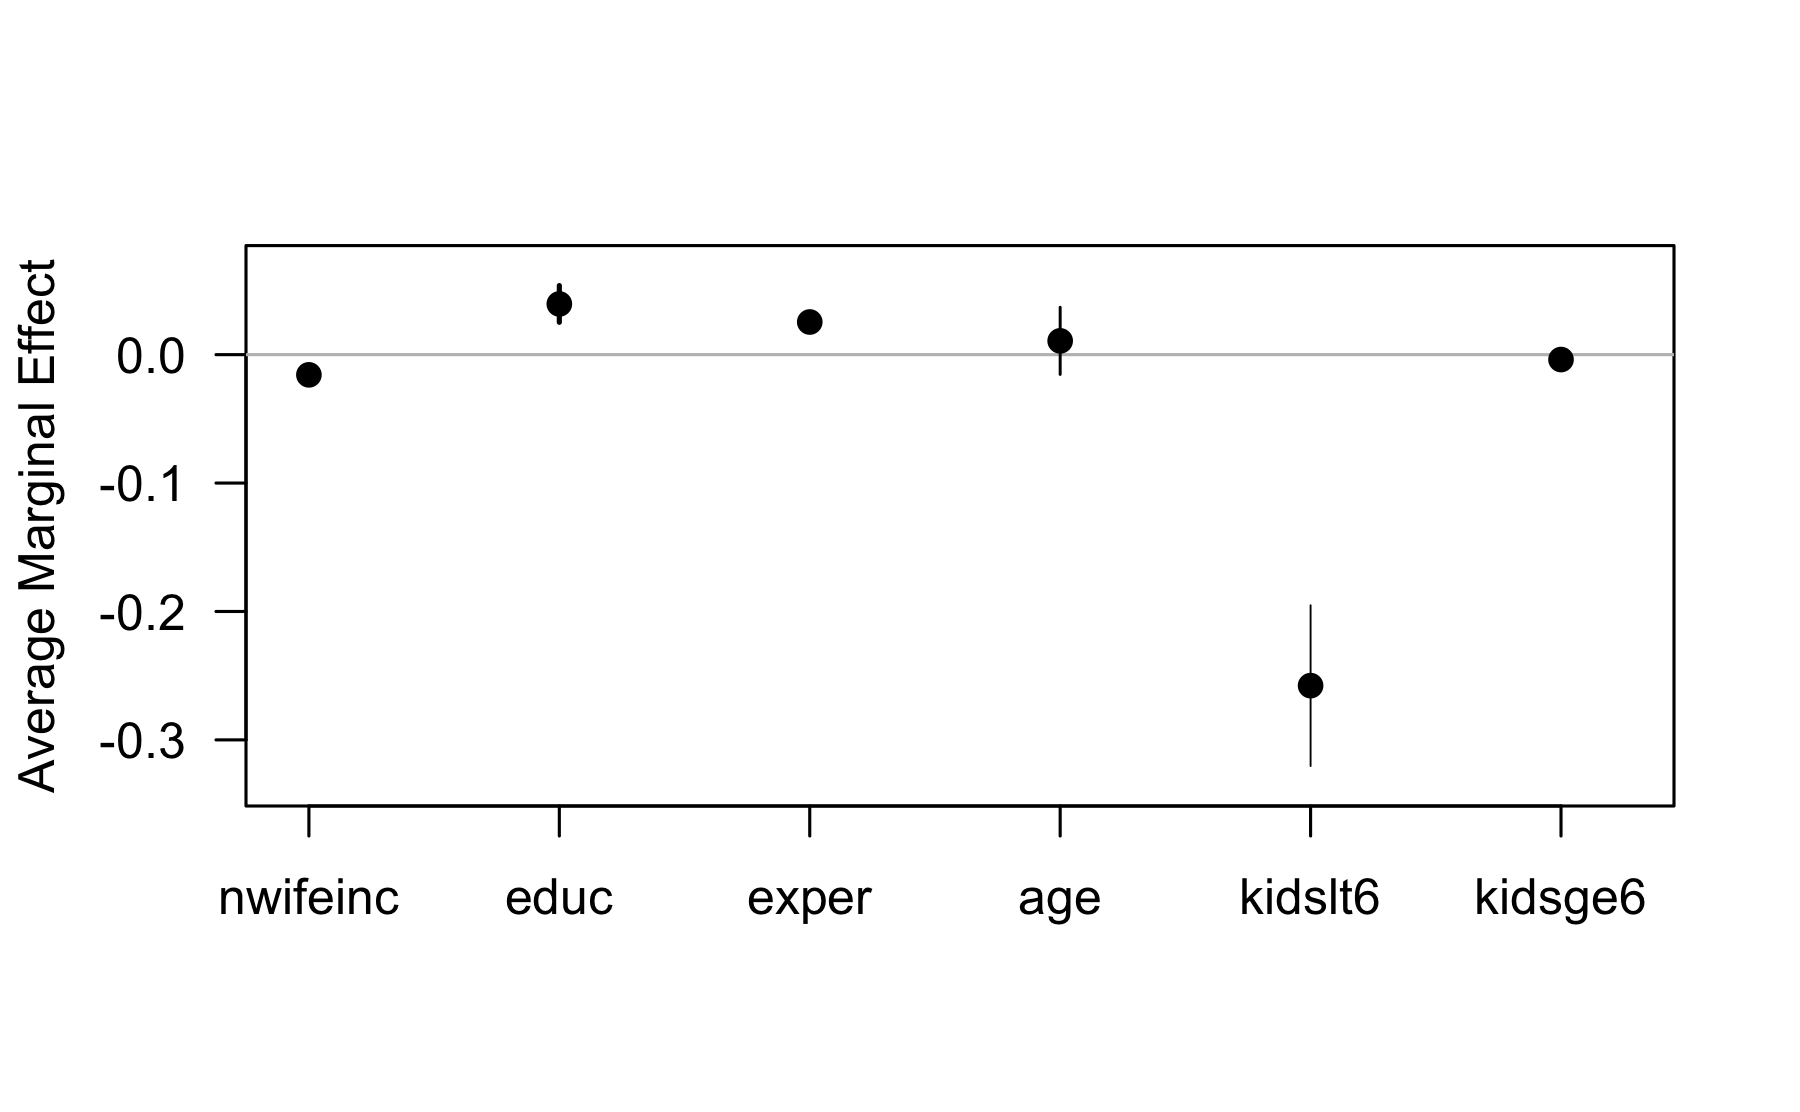
\includegraphics{MEM5220_R_files/figure-latex/unnamed-chunk-181-1.pdf}

\begin{Shaded}
\begin{Highlighting}[]
\CommentTok{#Some functions to characterise time series}
\CommentTok{#Position in the cycle}
\KeywordTok{cycle}\NormalTok{(cpits)}
\end{Highlighting}
\end{Shaded}

\begin{verbatim}
##      Jan Feb Mar Apr May Jun Jul Aug Sep Oct Nov Dec
## 1996   1   2   3   4   5   6   7   8   9  10  11  12
## 1997   1   2   3   4   5   6   7   8   9  10  11  12
## 1998   1   2   3   4   5   6   7   8   9  10  11  12
## 1999   1   2   3   4   5   6   7   8   9  10  11  12
## 2000   1   2   3   4   5   6   7   8   9  10  11  12
## 2001   1   2   3   4   5   6   7   8   9  10  11  12
## 2002   1   2   3   4   5   6   7   8   9  10  11  12
## 2003   1   2   3   4   5   6   7   8   9  10  11  12
## 2004   1   2   3   4   5   6   7   8   9  10  11  12
## 2005   1   2   3   4   5   6   7   8   9  10  11  12
## 2006   1   2   3   4   5   6   7   8   9  10  11  12
## 2007   1   2   3   4   5   6   7   8   9  10  11  12
## 2008   1   2   3   4   5   6   7   8   9  10  11  12
## 2009   1   2   3   4   5   6   7   8   9  10  11  12
## 2010   1   2   3   4   5   6   7   8   9  10  11  12
## 2011   1   2   3   4   5   6   7   8   9  10  11  12
## 2012   1   2   3   4   5   6   7   8   9  10  11  12
## 2013   1   2   3   4   5   6   7   8   9  10  11  12
## 2014   1   2   3   4   5   6   7   8   9  10  11  12
## 2015   1   2   3   4   5   6   7   8   9  10  11  12
## 2016   1   2   3   4   5   6   7   8   9  10  11  12
## 2017   1   2   3   4   5   6   7   8   9  10  11  12
## 2018   1   2   3   4   5   6   7   8   9
\end{verbatim}

\begin{Shaded}
\begin{Highlighting}[]
\CommentTok{#to check frequency}
\KeywordTok{frequency}\NormalTok{(cpits)}
\end{Highlighting}
\end{Shaded}

\begin{verbatim}
## [1] 12
\end{verbatim}

\begin{Shaded}
\begin{Highlighting}[]
\CommentTok{#How time is represented? As a fraction of the year!}
\KeywordTok{time}\NormalTok{(cpits)}
\end{Highlighting}
\end{Shaded}

\begin{verbatim}
##           Jan      Feb      Mar      Apr      May      Jun      Jul
## 1996 1996.000 1996.083 1996.167 1996.250 1996.333 1996.417 1996.500
## 1997 1997.000 1997.083 1997.167 1997.250 1997.333 1997.417 1997.500
## 1998 1998.000 1998.083 1998.167 1998.250 1998.333 1998.417 1998.500
## 1999 1999.000 1999.083 1999.167 1999.250 1999.333 1999.417 1999.500
## 2000 2000.000 2000.083 2000.167 2000.250 2000.333 2000.417 2000.500
## 2001 2001.000 2001.083 2001.167 2001.250 2001.333 2001.417 2001.500
## 2002 2002.000 2002.083 2002.167 2002.250 2002.333 2002.417 2002.500
## 2003 2003.000 2003.083 2003.167 2003.250 2003.333 2003.417 2003.500
## 2004 2004.000 2004.083 2004.167 2004.250 2004.333 2004.417 2004.500
## 2005 2005.000 2005.083 2005.167 2005.250 2005.333 2005.417 2005.500
## 2006 2006.000 2006.083 2006.167 2006.250 2006.333 2006.417 2006.500
## 2007 2007.000 2007.083 2007.167 2007.250 2007.333 2007.417 2007.500
## 2008 2008.000 2008.083 2008.167 2008.250 2008.333 2008.417 2008.500
## 2009 2009.000 2009.083 2009.167 2009.250 2009.333 2009.417 2009.500
## 2010 2010.000 2010.083 2010.167 2010.250 2010.333 2010.417 2010.500
## 2011 2011.000 2011.083 2011.167 2011.250 2011.333 2011.417 2011.500
## 2012 2012.000 2012.083 2012.167 2012.250 2012.333 2012.417 2012.500
## 2013 2013.000 2013.083 2013.167 2013.250 2013.333 2013.417 2013.500
## 2014 2014.000 2014.083 2014.167 2014.250 2014.333 2014.417 2014.500
## 2015 2015.000 2015.083 2015.167 2015.250 2015.333 2015.417 2015.500
## 2016 2016.000 2016.083 2016.167 2016.250 2016.333 2016.417 2016.500
## 2017 2017.000 2017.083 2017.167 2017.250 2017.333 2017.417 2017.500
## 2018 2018.000 2018.083 2018.167 2018.250 2018.333 2018.417 2018.500
##           Aug      Sep      Oct      Nov      Dec
## 1996 1996.583 1996.667 1996.750 1996.833 1996.917
## 1997 1997.583 1997.667 1997.750 1997.833 1997.917
## 1998 1998.583 1998.667 1998.750 1998.833 1998.917
## 1999 1999.583 1999.667 1999.750 1999.833 1999.917
## 2000 2000.583 2000.667 2000.750 2000.833 2000.917
## 2001 2001.583 2001.667 2001.750 2001.833 2001.917
## 2002 2002.583 2002.667 2002.750 2002.833 2002.917
## 2003 2003.583 2003.667 2003.750 2003.833 2003.917
## 2004 2004.583 2004.667 2004.750 2004.833 2004.917
## 2005 2005.583 2005.667 2005.750 2005.833 2005.917
## 2006 2006.583 2006.667 2006.750 2006.833 2006.917
## 2007 2007.583 2007.667 2007.750 2007.833 2007.917
## 2008 2008.583 2008.667 2008.750 2008.833 2008.917
## 2009 2009.583 2009.667 2009.750 2009.833 2009.917
## 2010 2010.583 2010.667 2010.750 2010.833 2010.917
## 2011 2011.583 2011.667 2011.750 2011.833 2011.917
## 2012 2012.583 2012.667 2012.750 2012.833 2012.917
## 2013 2013.583 2013.667 2013.750 2013.833 2013.917
## 2014 2014.583 2014.667 2014.750 2014.833 2014.917
## 2015 2015.583 2015.667 2015.750 2015.833 2015.917
## 2016 2016.583 2016.667 2016.750 2016.833 2016.917
## 2017 2017.583 2017.667 2017.750 2017.833 2017.917
## 2018 2018.583 2018.667
\end{verbatim}

\begin{Shaded}
\begin{Highlighting}[]
\CommentTok{#average difference between time units (0.08333 years or =1/12)}
\KeywordTok{deltat}\NormalTok{(cpits)}
\end{Highlighting}
\end{Shaded}

\begin{verbatim}
## [1] 0.08333333
\end{verbatim}

\begin{Shaded}
\begin{Highlighting}[]
\CommentTok{#Let's plot four graphs in 2x2}
\KeywordTok{par}\NormalTok{(}\DataTypeTok{mfrow=}\KeywordTok{c}\NormalTok{(}\DecValTok{2}\NormalTok{,}\DecValTok{2}\NormalTok{))}
\KeywordTok{plot}\NormalTok{(cpits)}
\KeywordTok{plot}\NormalTok{(}\KeywordTok{log}\NormalTok{(cpits))}
\CommentTok{#monthly growth rate}
\KeywordTok{plot}\NormalTok{(}\KeywordTok{diff}\NormalTok{(}\KeywordTok{log}\NormalTok{(cpits)))}
\CommentTok{#annual growth rate}
\KeywordTok{plot}\NormalTok{(}\KeywordTok{diff}\NormalTok{(}\KeywordTok{log}\NormalTok{(cpits), }\DataTypeTok{lag=}\DecValTok{12}\NormalTok{))}
\end{Highlighting}
\end{Shaded}

\includegraphics{MEM5220_R_files/figure-latex/unnamed-chunk-181-2.pdf}

\begin{Shaded}
\begin{Highlighting}[]
\CommentTok{#close the graph}
\KeywordTok{dev.off}\NormalTok{()}
\end{Highlighting}
\end{Shaded}

\begin{verbatim}
## null device 
##           1
\end{verbatim}

\hypertarget{exponential-smoothing-and-forecasting}{%
\section{Exponential smoothing and
forecasting}\label{exponential-smoothing-and-forecasting}}

Let's forecast monthly inflation rate based using Holt-Winters
exponential smoothing with trend and additive seasonal component. Note
that we must not have missing data.

\begin{Shaded}
\begin{Highlighting}[]
\NormalTok{dlcpi <-}\StringTok{ }\KeywordTok{diff}\NormalTok{(}\KeywordTok{log}\NormalTok{(cpits), }\DataTypeTok{lag=}\DecValTok{1}\NormalTok{)}
\CommentTok{#omit missing values, we had one in October 2018}
\NormalTok{dlcpi <-}\StringTok{ }\KeywordTok{na.omit}\NormalTok{(dlcpi)}
\KeywordTok{plot}\NormalTok{(dlcpi)}
\end{Highlighting}
\end{Shaded}

\includegraphics{MEM5220_R_files/figure-latex/unnamed-chunk-182-1.pdf}

\begin{Shaded}
\begin{Highlighting}[]
\CommentTok{#Additive Holt-Winters}
\NormalTok{(m <-}\StringTok{ }\KeywordTok{HoltWinters}\NormalTok{(dlcpi, }\DataTypeTok{seasonal =} \StringTok{"additive"}\NormalTok{))}
\end{Highlighting}
\end{Shaded}

\begin{verbatim}
## Holt-Winters exponential smoothing with trend and additive seasonal component.
## 
## Call:
## HoltWinters(x = dlcpi, seasonal = "additive")
## 
## Smoothing parameters:
##  alpha: 0.2223446
##  beta : 0.01158144
##  gamma: 0.4079999
## 
## Coefficients:
##              [,1]
## a    5.980743e-03
## b    2.555965e-05
## s1  -6.449780e-03
## s2  -4.597118e-03
## s3  -5.897731e-03
## s4  -2.844368e-03
## s5   5.123452e-03
## s6  -3.167743e-04
## s7   3.546006e-04
## s8  -3.146611e-04
## s9   1.824240e-04
## s10 -2.654886e-03
## s11 -2.217077e-03
## s12 -7.249312e-03
\end{verbatim}

\begin{Shaded}
\begin{Highlighting}[]
\KeywordTok{plot}\NormalTok{(m)}
\end{Highlighting}
\end{Shaded}

\includegraphics{MEM5220_R_files/figure-latex/unnamed-chunk-182-2.pdf}

\begin{Shaded}
\begin{Highlighting}[]
\CommentTok{#Predict 12 months ahead}
\NormalTok{p <-}\StringTok{ }\KeywordTok{predict}\NormalTok{(m, }\DataTypeTok{n.ahead =} \DecValTok{12}\NormalTok{, }\DataTypeTok{prediction.interval =} \OtherTok{TRUE}\NormalTok{)}
\KeywordTok{plot}\NormalTok{(m, p)}
\end{Highlighting}
\end{Shaded}

\includegraphics{MEM5220_R_files/figure-latex/unnamed-chunk-182-3.pdf}

\hypertarget{arima-models}{%
\section{ARIMA models}\label{arima-models}}

We use functions \texttt{arima} from \texttt{stats} package,
\texttt{auto.arima} and \texttt{Arima} from \texttt{forecast} package.
We also look at autocorrelation functions and partial autocorrelation
functions with \texttt{acf2} command from \texttt{astsa} package.

ARMA models are suited to describe stationary time series. Wold's
composition says that every covariance-stationary time series can be
represented as a linear combination of lags of white noise (and a
deterministic time series).

\[
X_t = W_t + a_1 \times W_{-1}+ a_2 \times W_{-2} + \dots
\]

If the time series is not stationary, we need to take first difference
of the series.

ARIMA models are denoted by ARIMA(p,d,q) where p is the order of AR
terms, q is the order of MA terms and d is the order of integration.
Full seasonal model is denoted by SARIMA(p,d,q) \(\times\) (P,D,Q)S
where capital letters denote respective the seasonal orders.

\hypertarget{simulation-of-arima-models}{%
\subsection{Simulation of ARIMA
models}\label{simulation-of-arima-models}}

To simulate ARMA models we use function \texttt{arima.sim}.

\begin{Shaded}
\begin{Highlighting}[]
\CommentTok{#To simulate ARIMA process}
\CommentTok{#MA(1) process}
\NormalTok{xma1 <-}\StringTok{ }\KeywordTok{arima.sim}\NormalTok{(}\KeywordTok{list}\NormalTok{(}\DataTypeTok{order=}\KeywordTok{c}\NormalTok{(}\DecValTok{0}\NormalTok{,}\DecValTok{0}\NormalTok{,}\DecValTok{1}\NormalTok{), }\DataTypeTok{ma=}\FloatTok{0.9}\NormalTok{), }\DataTypeTok{n=}\DecValTok{100}\NormalTok{)}
\KeywordTok{plot}\NormalTok{(xma1)}
\end{Highlighting}
\end{Shaded}

\includegraphics{MEM5220_R_files/figure-latex/unnamed-chunk-184-1.pdf}

\begin{Shaded}
\begin{Highlighting}[]
\CommentTok{#AR(1)}
\NormalTok{xar1 <-}\StringTok{ }\KeywordTok{arima.sim}\NormalTok{(}\KeywordTok{list}\NormalTok{(}\DataTypeTok{order=}\KeywordTok{c}\NormalTok{(}\DecValTok{1}\NormalTok{,}\DecValTok{0}\NormalTok{,}\DecValTok{0}\NormalTok{), }\DataTypeTok{ar=}\FloatTok{0.8}\NormalTok{), }\DataTypeTok{n=}\DecValTok{100}\NormalTok{)}
\KeywordTok{plot}\NormalTok{(xar1)}
\end{Highlighting}
\end{Shaded}

\includegraphics{MEM5220_R_files/figure-latex/unnamed-chunk-184-2.pdf}

\begin{Shaded}
\begin{Highlighting}[]
\CommentTok{#ARMA(1,1)}
\NormalTok{xarma11 <-}\StringTok{ }\KeywordTok{arima.sim}\NormalTok{(}\KeywordTok{list}\NormalTok{(}\DataTypeTok{order=}\KeywordTok{c}\NormalTok{(}\DecValTok{1}\NormalTok{,}\DecValTok{0}\NormalTok{,}\DecValTok{1}\NormalTok{), }\DataTypeTok{ar=}\FloatTok{0.8}\NormalTok{, }\DataTypeTok{ma=}\FloatTok{0.5}\NormalTok{), }\DataTypeTok{n=}\DecValTok{100}\NormalTok{)}
\KeywordTok{plot}\NormalTok{(xarma11)}
\end{Highlighting}
\end{Shaded}

\includegraphics{MEM5220_R_files/figure-latex/unnamed-chunk-184-3.pdf}

\begin{Shaded}
\begin{Highlighting}[]
\CommentTok{#ARMA(2,1)}
\NormalTok{xarma21 <-}\StringTok{ }\KeywordTok{arima.sim}\NormalTok{(}\KeywordTok{list}\NormalTok{(}\DataTypeTok{order=}\KeywordTok{c}\NormalTok{(}\DecValTok{2}\NormalTok{,}\DecValTok{0}\NormalTok{,}\DecValTok{1}\NormalTok{), }\DataTypeTok{ar=}\KeywordTok{c}\NormalTok{(}\FloatTok{0.8}\NormalTok{,}\OperatorTok{-}\FloatTok{0.5}\NormalTok{), }\DataTypeTok{ma=}\FloatTok{0.5}\NormalTok{), }\DataTypeTok{n=}\DecValTok{100}\NormalTok{)}
\KeywordTok{plot}\NormalTok{(xarma21)}
\end{Highlighting}
\end{Shaded}

\includegraphics{MEM5220_R_files/figure-latex/unnamed-chunk-184-4.pdf}

\hypertarget{acf-and-pacf}{%
\subsection{ACF and PACF}\label{acf-and-pacf}}

Next let's have a quick look how to identify ARMA model from the data.
Very difficult to distinguish from the graphs, therefore we also use
autocorrelation functions (ACF) and partial autocorrelation functions
(PACF).

\begin{Shaded}
\begin{Highlighting}[]
\CommentTok{#Compare the following time series in the graph}
\NormalTok{x <-}\StringTok{ }\KeywordTok{arima.sim}\NormalTok{(}\KeywordTok{list}\NormalTok{(}\DataTypeTok{order=}\KeywordTok{c}\NormalTok{(}\DecValTok{1}\NormalTok{,}\DecValTok{0}\NormalTok{,}\DecValTok{0}\NormalTok{), }\DataTypeTok{ar=}\OperatorTok{-}\NormalTok{.}\DecValTok{7}\NormalTok{), }\DataTypeTok{n=}\DecValTok{200}\NormalTok{)}
\NormalTok{y <-}\StringTok{ }\KeywordTok{arima.sim}\NormalTok{(}\KeywordTok{list}\NormalTok{(}\DataTypeTok{order=}\KeywordTok{c}\NormalTok{(}\DecValTok{0}\NormalTok{,}\DecValTok{0}\NormalTok{,}\DecValTok{1}\NormalTok{), }\DataTypeTok{ma=}\OperatorTok{-}\NormalTok{.}\DecValTok{7}\NormalTok{), }\DataTypeTok{n=}\DecValTok{200}\NormalTok{)}

\KeywordTok{par}\NormalTok{(}\DataTypeTok{mfrow=}\KeywordTok{c}\NormalTok{(}\DecValTok{1}\NormalTok{,}\DecValTok{2}\NormalTok{))}
\KeywordTok{plot}\NormalTok{(x, }\DataTypeTok{main =} \StringTok{"AR(1)"}\NormalTok{)}
\KeywordTok{plot}\NormalTok{(y, }\DataTypeTok{main =} \StringTok{"MA(1)"}\NormalTok{)}
\end{Highlighting}
\end{Shaded}

\includegraphics{MEM5220_R_files/figure-latex/unnamed-chunk-185-1.pdf}

\begin{Shaded}
\begin{Highlighting}[]
\KeywordTok{dev.off}\NormalTok{()}
\end{Highlighting}
\end{Shaded}

\begin{verbatim}
## null device 
##           1
\end{verbatim}

Autocorrelation function and partial autocorrelation function help to
identify lag structure of ARMA models. If pure AR(p) process then ACF
will tail off (changes to smaller) and PACF cuts off lag p.~If pure
MA(q) process then PACF will tail off (changes to smaller) and ACF cuts
off lag q. If ARMA(p,q) then both ACF and PACF will tail off. Then start
from (ARMA(1,1) and add more lags as needed).

Look at the following ACF and PACF functions and see if the ACF and PACF
of the simulated time series follow expected pattern.

\begin{Shaded}
\begin{Highlighting}[]
\CommentTok{#AR(1)}
\NormalTok{x <-}\StringTok{ }\KeywordTok{arima.sim}\NormalTok{(}\KeywordTok{list}\NormalTok{(}\DataTypeTok{order=}\KeywordTok{c}\NormalTok{(}\DecValTok{1}\NormalTok{,}\DecValTok{0}\NormalTok{,}\DecValTok{0}\NormalTok{), }\DataTypeTok{ar=}\KeywordTok{c}\NormalTok{(}\FloatTok{0.9}\NormalTok{)), }\DataTypeTok{n=}\DecValTok{100}\NormalTok{)}
\KeywordTok{plot}\NormalTok{(x,}\DataTypeTok{main=}\StringTok{"AR(1)"}\NormalTok{) }
\end{Highlighting}
\end{Shaded}

\includegraphics{MEM5220_R_files/figure-latex/unnamed-chunk-186-1.pdf}

\begin{Shaded}
\begin{Highlighting}[]
\CommentTok{#ACF, PACF from atsta package}
\KeywordTok{acf2}\NormalTok{(x)}
\end{Highlighting}
\end{Shaded}

\includegraphics{MEM5220_R_files/figure-latex/unnamed-chunk-186-2.pdf}

\begin{verbatim}
##         ACF  PACF
##  [1,]  0.76  0.76
##  [2,]  0.58 -0.01
##  [3,]  0.42 -0.04
##  [4,]  0.25 -0.14
##  [5,]  0.11 -0.04
##  [6,]  0.06  0.07
##  [7,]  0.04  0.06
##  [8,] -0.01 -0.13
##  [9,] -0.07 -0.10
## [10,] -0.12 -0.05
## [11,] -0.12  0.09
## [12,] -0.12  0.03
## [13,] -0.09  0.00
## [14,] -0.07 -0.05
## [15,] -0.08 -0.10
## [16,] -0.12 -0.06
## [17,] -0.16 -0.03
## [18,] -0.18 -0.01
## [19,] -0.15  0.07
## [20,] -0.19 -0.20
\end{verbatim}

\begin{Shaded}
\begin{Highlighting}[]
\CommentTok{#Look the autocorrelation coefficients}

\CommentTok{#AR(2)}
\NormalTok{x <-}\StringTok{ }\KeywordTok{arima.sim}\NormalTok{(}\KeywordTok{list}\NormalTok{(}\DataTypeTok{order=}\KeywordTok{c}\NormalTok{(}\DecValTok{2}\NormalTok{,}\DecValTok{0}\NormalTok{,}\DecValTok{0}\NormalTok{), }\DataTypeTok{ar=}\KeywordTok{c}\NormalTok{(}\FloatTok{0.9}\NormalTok{, }\FloatTok{-0.4}\NormalTok{)), }\DataTypeTok{n=}\DecValTok{100}\NormalTok{)}
\KeywordTok{plot}\NormalTok{(x, }\DataTypeTok{main=}\StringTok{"AR(2)"}\NormalTok{) }
\end{Highlighting}
\end{Shaded}

\includegraphics{MEM5220_R_files/figure-latex/unnamed-chunk-186-3.pdf}

\begin{Shaded}
\begin{Highlighting}[]
\KeywordTok{acf2}\NormalTok{(x)}
\end{Highlighting}
\end{Shaded}

\includegraphics{MEM5220_R_files/figure-latex/unnamed-chunk-186-4.pdf}

\begin{verbatim}
##         ACF  PACF
##  [1,]  0.59  0.59
##  [2,]  0.04 -0.47
##  [3,] -0.30 -0.10
##  [4,] -0.27  0.11
##  [5,] -0.12 -0.11
##  [6,] -0.05 -0.11
##  [7,] -0.04  0.01
##  [8,] -0.10 -0.16
##  [9,] -0.16 -0.13
## [10,] -0.16 -0.05
## [11,] -0.09 -0.05
## [12,] -0.01 -0.11
## [13,]  0.05  0.00
## [14,]  0.03 -0.12
## [15,]  0.04  0.04
## [16,]  0.07  0.01
## [17,]  0.20  0.17
## [18,]  0.22 -0.04
## [19,]  0.09 -0.07
## [20,] -0.10 -0.05
\end{verbatim}

\begin{Shaded}
\begin{Highlighting}[]
\CommentTok{#MA(1)}
\NormalTok{x <-}\StringTok{ }\KeywordTok{arima.sim}\NormalTok{(}\KeywordTok{list}\NormalTok{(}\DataTypeTok{order=}\KeywordTok{c}\NormalTok{(}\DecValTok{0}\NormalTok{,}\DecValTok{0}\NormalTok{,}\DecValTok{1}\NormalTok{), }\DataTypeTok{ma=}\FloatTok{0.4}\NormalTok{), }\DataTypeTok{n=}\DecValTok{100}\NormalTok{)}
\KeywordTok{plot}\NormalTok{(x, }\DataTypeTok{main=}\StringTok{"MA(1)"}\NormalTok{) }
\end{Highlighting}
\end{Shaded}

\includegraphics{MEM5220_R_files/figure-latex/unnamed-chunk-186-5.pdf}

\begin{Shaded}
\begin{Highlighting}[]
\KeywordTok{acf2}\NormalTok{(x)}
\end{Highlighting}
\end{Shaded}

\includegraphics{MEM5220_R_files/figure-latex/unnamed-chunk-186-6.pdf}

\begin{verbatim}
##         ACF  PACF
##  [1,]  0.28  0.28
##  [2,] -0.13 -0.23
##  [3,] -0.08  0.04
##  [4,] -0.02 -0.05
##  [5,] -0.02 -0.02
##  [6,]  0.02  0.03
##  [7,] -0.04 -0.08
##  [8,] -0.12 -0.09
##  [9,] -0.02  0.04
## [10,]  0.06  0.01
## [11,] -0.06 -0.10
## [12,]  0.01  0.09
## [13,]  0.06 -0.01
## [14,] -0.10 -0.12
## [15,] -0.07  0.02
## [16,]  0.04  0.01
## [17,] -0.02 -0.06
## [18,]  0.01  0.06
## [19,]  0.10  0.05
## [20,]  0.00 -0.05
\end{verbatim}

\begin{Shaded}
\begin{Highlighting}[]
\CommentTok{#ARMA(1,1)}
\NormalTok{x <-}\StringTok{ }\KeywordTok{arima.sim}\NormalTok{(}\KeywordTok{list}\NormalTok{(}\DataTypeTok{order=}\KeywordTok{c}\NormalTok{(}\DecValTok{1}\NormalTok{,}\DecValTok{0}\NormalTok{,}\DecValTok{1}\NormalTok{), }\DataTypeTok{ar=}\FloatTok{0.9}\NormalTok{, }\DataTypeTok{ma=}\OperatorTok{-}\FloatTok{0.4}\NormalTok{), }\DataTypeTok{n=}\DecValTok{200}\NormalTok{)}
\KeywordTok{plot}\NormalTok{(x, }\DataTypeTok{main=}\StringTok{"ARMA(1,1)"}\NormalTok{) }
\end{Highlighting}
\end{Shaded}

\includegraphics{MEM5220_R_files/figure-latex/unnamed-chunk-186-7.pdf}

\begin{Shaded}
\begin{Highlighting}[]
\KeywordTok{acf2}\NormalTok{(x)}
\end{Highlighting}
\end{Shaded}

\includegraphics{MEM5220_R_files/figure-latex/unnamed-chunk-186-8.pdf}

\begin{verbatim}
##         ACF  PACF
##  [1,]  0.76  0.76
##  [2,]  0.64  0.14
##  [3,]  0.57  0.11
##  [4,]  0.52  0.06
##  [5,]  0.43 -0.08
##  [6,]  0.32 -0.11
##  [7,]  0.27  0.02
##  [8,]  0.21 -0.02
##  [9,]  0.20  0.09
## [10,]  0.15 -0.04
## [11,]  0.11 -0.04
## [12,]  0.09  0.02
## [13,]  0.07 -0.04
## [14,]  0.02 -0.06
## [15,] -0.03 -0.07
## [16,] -0.05  0.01
## [17,] -0.09 -0.07
## [18,] -0.10  0.04
## [19,] -0.13 -0.04
## [20,] -0.10  0.11
## [21,] -0.10 -0.02
## [22,] -0.11 -0.04
## [23,] -0.13 -0.06
## [24,] -0.13 -0.02
## [25,] -0.11  0.02
\end{verbatim}

\hypertarget{estimation-of-arima-models}{%
\subsection{Estimation of ARIMA
models}\label{estimation-of-arima-models}}

Let's simulate a model and then estimate it with \texttt{arima} and
\texttt{sarima} commands.

\begin{Shaded}
\begin{Highlighting}[]
\CommentTok{#generate AR(2) process with mean}
\NormalTok{x <-}\StringTok{ }\KeywordTok{arima.sim}\NormalTok{(}\KeywordTok{list}\NormalTok{(}\DataTypeTok{order=}\KeywordTok{c}\NormalTok{(}\DecValTok{2}\NormalTok{,}\DecValTok{0}\NormalTok{,}\DecValTok{0}\NormalTok{), }
                    \DataTypeTok{ar=}\KeywordTok{c}\NormalTok{(}\FloatTok{1.5}\NormalTok{, }\FloatTok{-.75}\NormalTok{)), }
               \DataTypeTok{n=}\DecValTok{200}\NormalTok{) }\OperatorTok{+}\StringTok{ }\DecValTok{50}


\KeywordTok{plot}\NormalTok{(x) }
\end{Highlighting}
\end{Shaded}

\includegraphics{MEM5220_R_files/figure-latex/unnamed-chunk-187-1.pdf}

\begin{Shaded}
\begin{Highlighting}[]
\CommentTok{#use command sarima from astsa package}
\CommentTok{#it provides a nice graph for residual diagnostics of the model}
\NormalTok{x_fit <-}\StringTok{ }\KeywordTok{sarima}\NormalTok{(x, }\DataTypeTok{p=}\DecValTok{2}\NormalTok{, }\DataTypeTok{d=}\DecValTok{0}\NormalTok{, }\DataTypeTok{q=}\DecValTok{0}\NormalTok{)}
\end{Highlighting}
\end{Shaded}

\begin{verbatim}
## initial  value 1.055937 
## iter   2 value 0.903084
## iter   3 value 0.522531
## iter   4 value 0.326178
## iter   5 value 0.191550
## iter   6 value 0.049617
## iter   7 value 0.035394
## iter   8 value 0.028680
## iter   9 value 0.028215
## iter  10 value 0.027723
## iter  11 value 0.027661
## iter  12 value 0.027660
## iter  13 value 0.027659
## iter  13 value 0.027659
## iter  13 value 0.027659
## final  value 0.027659 
## converged
## initial  value 0.032953 
## iter   2 value 0.032946
## iter   3 value 0.032938
## iter   4 value 0.032937
## iter   5 value 0.032937
## iter   6 value 0.032937
## iter   7 value 0.032937
## iter   7 value 0.032937
## iter   7 value 0.032937
## final  value 0.032937 
## converged
\end{verbatim}

\includegraphics{MEM5220_R_files/figure-latex/unnamed-chunk-187-2.pdf}

\begin{Shaded}
\begin{Highlighting}[]
\NormalTok{x_fit}\OperatorTok{$}\NormalTok{ttable}
\end{Highlighting}
\end{Shaded}

\begin{verbatim}
##       Estimate     SE  t.value p.value
## ar1     1.4669 0.0458  31.9940       0
## ar2    -0.7528 0.0456 -16.4925       0
## xmean  50.2442 0.2540 197.8043       0
\end{verbatim}

\begin{Shaded}
\begin{Highlighting}[]
\CommentTok{# => residuals are white noise}

\CommentTok{#alternatively may use command arima from the stats package}
\NormalTok{x_fit2 <-}\StringTok{ }\KeywordTok{arima}\NormalTok{(x, }\DataTypeTok{order=}\KeywordTok{c}\NormalTok{(}\DecValTok{2}\NormalTok{, }\DecValTok{0}\NormalTok{, }\DecValTok{0}\NormalTok{))}
\NormalTok{x_fit2}
\end{Highlighting}
\end{Shaded}

\begin{verbatim}
## 
## Call:
## arima(x = x, order = c(2, 0, 0))
## 
## Coefficients:
##          ar1      ar2  intercept
##       1.4669  -0.7528    50.2442
## s.e.  0.0458   0.0456     0.2540
## 
## sigma^2 estimated as 1.053:  log likelihood = -290.38,  aic = 588.75
\end{verbatim}

\begin{Shaded}
\begin{Highlighting}[]
\CommentTok{#Let's have a quick look at residual diagnostics}
\KeywordTok{tsdiag}\NormalTok{(x_fit2)}
\end{Highlighting}
\end{Shaded}

\includegraphics{MEM5220_R_files/figure-latex/unnamed-chunk-187-3.pdf}

\begin{Shaded}
\begin{Highlighting}[]
\NormalTok{?Arima}
\NormalTok{x_fit3 <-}\StringTok{ }\KeywordTok{Arima}\NormalTok{(x, }\DataTypeTok{order=}\KeywordTok{c}\NormalTok{(}\DecValTok{2}\NormalTok{,}\DecValTok{0}\NormalTok{,}\DecValTok{0}\NormalTok{))}
\NormalTok{x_fit3}
\end{Highlighting}
\end{Shaded}

\begin{verbatim}
## Series: x 
## ARIMA(2,0,0) with non-zero mean 
## 
## Coefficients:
##          ar1      ar2     mean
##       1.4669  -0.7528  50.2442
## s.e.  0.0458   0.0456   0.2540
## 
## sigma^2 estimated as 1.069:  log likelihood=-290.38
## AIC=588.75   AICc=588.96   BIC=601.94
\end{verbatim}

\begin{Shaded}
\begin{Highlighting}[]
\KeywordTok{Arima}\NormalTok{(x, }\DataTypeTok{order=}\KeywordTok{c}\NormalTok{(}\DecValTok{2}\NormalTok{,}\DecValTok{0}\NormalTok{,}\DecValTok{0}\NormalTok{))  }\OperatorTok\StringTok{  }
\StringTok{  }\KeywordTok{forecast}\NormalTok{(}\DataTypeTok{h=}\DecValTok{20}\NormalTok{) }\OperatorTok
\StringTok{  }\NormalTok{autoplot}
\end{Highlighting}
\end{Shaded}

\includegraphics{MEM5220_R_files/figure-latex/unnamed-chunk-187-4.pdf}

\hypertarget{choosing-between-models}{%
\subsection{Choosing between models}\label{choosing-between-models}}

\begin{enumerate}
\def\labelenumi{\arabic{enumi})}
\tightlist
\item
  Descriptive power and simplicity Use AIC or BIC criteria, which both
  have penalty on model errors (average{[}(observed-predicted)\^{}2{]})
  and number of parameters (k*(p+q). The larger the AIC or BIC, the
  worse is the model. BIC has larger penalty on model parameters
  (k=ln(n)) than AIC (k=2), hence prefers simpler models.
\end{enumerate}

Goal: find the model with the smallest AIC or BIC.

\begin{enumerate}
\def\labelenumi{\arabic{enumi})}
\setcounter{enumi}{1}
\tightlist
\item
  Residual analysis Models residuals should be white noise, otherwise
  there is still some information left in the residuals.
\end{enumerate}

sarima() function provides graphical analysis of residuals: a)
standardised residuals - are there obvious patterns in the residuals? b)
ACF of residuals - any remaining correlation in residuals c) Normal Q-Q
plot - if residuals are normal, then they should be along the line. It
would be nice to have normal errors to rely on t-distribution, but that
is not so large problem if violated (Caution: I am not an expert!) d)
Ljung-Box Q-statistic p-values - points must above the line in order to
have statistically insignificant test-statistics.

The standardized residuals should behave as a white noise sequence with
mean zero and variance one. The sample ACF of the residuals should also
look like that of white noise. Normality is important assumption when
fitting ARMA models. Examine the Q-Q plot for departures from normality
and to identify outliers.

\begin{Shaded}
\begin{Highlighting}[]
\CommentTok{## to compare models use BIC() and AIC() statistics; BIC() and AIC() would choose the smallest}
\CommentTok{#Let's estimate two models}
\CommentTok{#AR(2)}
\NormalTok{x_fit2 <-}\StringTok{ }\KeywordTok{arima}\NormalTok{(x, }\DataTypeTok{order=}\KeywordTok{c}\NormalTok{(}\DecValTok{2}\NormalTok{, }\DecValTok{0}\NormalTok{, }\DecValTok{0}\NormalTok{))}
\CommentTok{#AR(3)}
\NormalTok{x_fit3 <-}\StringTok{ }\KeywordTok{arima}\NormalTok{(x, }\DataTypeTok{order=}\KeywordTok{c}\NormalTok{(}\DecValTok{3}\NormalTok{, }\DecValTok{0}\NormalTok{, }\DecValTok{1}\NormalTok{))}
\NormalTok{x_fit3}
\end{Highlighting}
\end{Shaded}

\begin{verbatim}
## 
## Call:
## arima(x = x, order = c(3, 0, 1))
## 
## Coefficients:
##          ar1      ar2      ar3     ma1  intercept
##       0.9969  -0.0840  -0.3293  0.5161    50.2437
## s.e.  0.5566   0.8242   0.4302  0.5387     0.2637
## 
## sigma^2 estimated as 1.048:  log likelihood = -289.93,  aic = 591.86
\end{verbatim}

\begin{Shaded}
\begin{Highlighting}[]
\KeywordTok{tsdiag}\NormalTok{(x_fit3)}
\end{Highlighting}
\end{Shaded}

\includegraphics{MEM5220_R_files/figure-latex/unnamed-chunk-188-1.pdf}

\begin{Shaded}
\begin{Highlighting}[]
\CommentTok{#Compare these models}
\KeywordTok{BIC}\NormalTok{(x_fit2, x_fit3) }\CommentTok{#=> x_fit2 better as BIC is smaller}
\end{Highlighting}
\end{Shaded}

\textbackslash{}begin\{table\}{[}h{]}
\textbackslash{}begin\{raggedright\}

\providecommand{\huxb}[2][0,0,0]{\arrayrulecolor[RGB]{#1}\global\arrayrulewidth=#2pt}
    \providecommand{\huxvb}[2][0,0,0]{\color[RGB]{#1}\vrule width #2pt}
    \providecommand{\huxtpad}[1]{\rule{0pt}{\baselineskip+#1}}
    \providecommand{\huxbpad}[1]{\rule[-#1]{0pt}{#1}}
  \begin{tabularx}{0.2\textwidth}{p{0.1\textwidth} p{0.1\textwidth}}


\par

\textbackslash{}end\{raggedright\} \textbackslash{}end\{table\}

\begin{Shaded}
\begin{Highlighting}[]
\KeywordTok{AIC}\NormalTok{(x_fit2, x_fit3) }\CommentTok{#=> x_fit2 still better in my case}
\end{Highlighting}
\end{Shaded}

\textbackslash{}begin\{table\}{[}h{]}
\textbackslash{}begin\{raggedright\}

\providecommand{\huxb}[2][0,0,0]{\arrayrulecolor[RGB]{#1}\global\arrayrulewidth=#2pt}
    \providecommand{\huxvb}[2][0,0,0]{\color[RGB]{#1}\vrule width #2pt}
    \providecommand{\huxtpad}[1]{\rule{0pt}{\baselineskip+#1}}
    \providecommand{\huxbpad}[1]{\rule[-#1]{0pt}{#1}}
  \begin{tabularx}{0.2\textwidth}{p{0.1\textwidth} p{0.1\textwidth}}


\par

\textbackslash{}end\{raggedright\} \textbackslash{}end\{table\}

\begin{Shaded}
\begin{Highlighting}[]
\CommentTok{#You may compare several models at once}
\KeywordTok{BIC}\NormalTok{(}\KeywordTok{arima}\NormalTok{(x, }\DataTypeTok{order=}\KeywordTok{c}\NormalTok{(}\DecValTok{1}\NormalTok{, }\DecValTok{0}\NormalTok{, }\DecValTok{0}\NormalTok{)), }
    \KeywordTok{arima}\NormalTok{(x, }\DataTypeTok{order=}\KeywordTok{c}\NormalTok{(}\DecValTok{2}\NormalTok{, }\DecValTok{0}\NormalTok{, }\DecValTok{0}\NormalTok{)), }\CommentTok{#=> this is best accoding to BIC}
    \KeywordTok{arima}\NormalTok{(x, }\DataTypeTok{order=}\KeywordTok{c}\NormalTok{(}\DecValTok{3}\NormalTok{, }\DecValTok{0}\NormalTok{, }\DecValTok{0}\NormalTok{)),}
    \KeywordTok{arima}\NormalTok{(x, }\DataTypeTok{order=}\KeywordTok{c}\NormalTok{(}\DecValTok{1}\NormalTok{, }\DecValTok{0}\NormalTok{, }\DecValTok{1}\NormalTok{)),}
    \KeywordTok{arima}\NormalTok{(x, }\DataTypeTok{order=}\KeywordTok{c}\NormalTok{(}\DecValTok{2}\NormalTok{, }\DecValTok{0}\NormalTok{, }\DecValTok{1}\NormalTok{)),}
    \KeywordTok{arima}\NormalTok{(x, }\DataTypeTok{order=}\KeywordTok{c}\NormalTok{(}\DecValTok{3}\NormalTok{, }\DecValTok{0}\NormalTok{, }\DecValTok{1}\NormalTok{)))}
\end{Highlighting}
\end{Shaded}

\textbackslash{}begin\{table\}{[}h{]}
\textbackslash{}begin\{raggedright\}

\providecommand{\huxb}[2][0,0,0]{\arrayrulecolor[RGB]{#1}\global\arrayrulewidth=#2pt}
    \providecommand{\huxvb}[2][0,0,0]{\color[RGB]{#1}\vrule width #2pt}
    \providecommand{\huxtpad}[1]{\rule{0pt}{\baselineskip+#1}}
    \providecommand{\huxbpad}[1]{\rule[-#1]{0pt}{#1}}
  \begin{tabularx}{0.2\textwidth}{p{0.1\textwidth} p{0.1\textwidth}}


\par

\textbackslash{}end\{raggedright\} \textbackslash{}end\{table\}

\hypertarget{automatic-esimation}{%
\subsection{Automatic esimation}\label{automatic-esimation}}

You may let \texttt{auto.arima} function to decide automatically which
model is the best one. It returns best ARIMA model according to either
AIC, AICc or BIC value. The function conducts a search over possible
model within the order constraints provided. See the help file for more
details. The function can also be used on non-stationary time series and
let it automatically test for unit roots.

\begin{Shaded}
\begin{Highlighting}[]
\NormalTok{forecast}\OperatorTok{::}\KeywordTok{auto.arima}\NormalTok{(x, }\DataTypeTok{d=}\DecValTok{0}\NormalTok{, }\DataTypeTok{max.p =} \DecValTok{5}\NormalTok{, }\DataTypeTok{max.q =} \DecValTok{5}\NormalTok{, }\DataTypeTok{ic=}\StringTok{"aic"}\NormalTok{)}
\end{Highlighting}
\end{Shaded}

\begin{verbatim}
## Series: x 
## ARIMA(2,0,0) with non-zero mean 
## 
## Coefficients:
##          ar1      ar2     mean
##       1.4669  -0.7528  50.2442
## s.e.  0.0458   0.0456   0.2540
## 
## sigma^2 estimated as 1.069:  log likelihood=-290.38
## AIC=588.75   AICc=588.96   BIC=601.94
\end{verbatim}

\begin{Shaded}
\begin{Highlighting}[]
\CommentTok{#surpisingly it ended up with ARMA(4,3) in my case when using AIC}

\CommentTok{#and AR(3) when using BIC, although AR(3) is not statistically significant}
\NormalTok{forecast}\OperatorTok{::}\KeywordTok{auto.arima}\NormalTok{(x, }\DataTypeTok{d=}\DecValTok{0}\NormalTok{, }\DataTypeTok{max.p =} \DecValTok{5}\NormalTok{, }\DataTypeTok{max.q =} \DecValTok{5}\NormalTok{, }\DataTypeTok{ic=}\StringTok{"bic"}\NormalTok{)}
\end{Highlighting}
\end{Shaded}

\begin{verbatim}
## Series: x 
## ARIMA(2,0,0) with non-zero mean 
## 
## Coefficients:
##          ar1      ar2     mean
##       1.4669  -0.7528  50.2442
## s.e.  0.0458   0.0456   0.2540
## 
## sigma^2 estimated as 1.069:  log likelihood=-290.38
## AIC=588.75   AICc=588.96   BIC=601.94
\end{verbatim}

\#\#\#Prediction with ARMA models

Prediction is straightforward, simply apply \texttt{predict} command to
the estimated model.

\begin{Shaded}
\begin{Highlighting}[]
\CommentTok{## An example of ARIMA forecasting three periods ahead:}
\KeywordTok{predict}\NormalTok{(x_fit2, }\DataTypeTok{n.ahead=} \DecValTok{3}\NormalTok{)}
\end{Highlighting}
\end{Shaded}

\begin{verbatim}
## $pred
## Time Series:
## Start = 201 
## End = 203 
## Frequency = 1 
## [1] 48.33845 48.73433 49.46398
## 
## $se
## Time Series:
## Start = 201 
## End = 203 
## Frequency = 1 
## [1] 1.026077 1.821600 2.319205
\end{verbatim}

\hypertarget{testing-for-unit-root}{%
\subsection{Testing for unit root}\label{testing-for-unit-root}}

To test for unit root we can use package \texttt{fUnitRoots}, which
includes Augmented Dickey Fuller unit root test and Phillips-Perron
test. We can also use package \texttt{urca}, which includes many tests.

\begin{Shaded}
\begin{Highlighting}[]
\CommentTok{#Let's first use again simulated time series}
\NormalTok{x1 <-}\StringTok{ }\KeywordTok{arima.sim}\NormalTok{(}\KeywordTok{list}\NormalTok{(}\DataTypeTok{order=}\KeywordTok{c}\NormalTok{(}\DecValTok{1}\NormalTok{,}\DecValTok{1}\NormalTok{,}\DecValTok{1}\NormalTok{), }\DataTypeTok{ar=}\KeywordTok{c}\NormalTok{(}\FloatTok{0.5}\NormalTok{), }\DataTypeTok{ma=}\OperatorTok{-}\FloatTok{0.3}\NormalTok{), }\DataTypeTok{n=}\DecValTok{100}\NormalTok{)}
\KeywordTok{plot}\NormalTok{(x1)}
\end{Highlighting}
\end{Shaded}

\includegraphics{MEM5220_R_files/figure-latex/unnamed-chunk-191-1.pdf}

\begin{Shaded}
\begin{Highlighting}[]
\CommentTok{#clearly random walk process}

\CommentTok{#Let's test using adfTest}
\CommentTok{#The null hypothesis is that time series is not stationary and we cannot reject that}
\KeywordTok{adfTest}\NormalTok{(x1)}
\end{Highlighting}
\end{Shaded}

\begin{verbatim}
## 
## Title:
##  Augmented Dickey-Fuller Test
## 
## Test Results:
##   PARAMETER:
##     Lag Order: 1
##   STATISTIC:
##     Dickey-Fuller: -0.998
##   P VALUE:
##     0.2951 
## 
## Description:
##  Sun Oct 28 21:27:56 2018 by user:
\end{verbatim}

\begin{Shaded}
\begin{Highlighting}[]
\CommentTok{#=> we cannot reject H0}

\CommentTok{#type of the regression:  "nc" no constant nor time trend, "c" with a constant but no time trend, "ct" with an intercept constant and a time trend. The default is "c".}
\KeywordTok{adfTest}\NormalTok{(x1, }\DataTypeTok{type=}\StringTok{"ct"}\NormalTok{)}
\end{Highlighting}
\end{Shaded}

\begin{verbatim}
## 
## Title:
##  Augmented Dickey-Fuller Test
## 
## Test Results:
##   PARAMETER:
##     Lag Order: 1
##   STATISTIC:
##     Dickey-Fuller: -3.0659
##   P VALUE:
##     0.1348 
## 
## Description:
##  Sun Oct 28 21:27:56 2018 by user:
\end{verbatim}

\begin{Shaded}
\begin{Highlighting}[]
\NormalTok{test1 <-}\StringTok{ }\KeywordTok{adfTest}\NormalTok{(x1, }\DataTypeTok{type=}\StringTok{"ct"}\NormalTok{)}
\CommentTok{#the model behind the test regression}
\KeywordTok{summary}\NormalTok{(test1}\OperatorTok{@}\NormalTok{test}\OperatorTok{$}\NormalTok{lm)}
\end{Highlighting}
\end{Shaded}

\begin{verbatim}
## 
## Call:
## lm(formula = y.diff ~ y.lag.1 + 1 + tt + y.diff.lag)
## 
## Residuals:
##     Min      1Q  Median      3Q     Max 
## -2.2753 -0.6501  0.0501  0.7262  3.1810 
## 
## Coefficients:
##              Estimate Std. Error t value Pr(>|t|)   
## (Intercept) -0.476773   0.263215  -1.811  0.07325 . 
## y.lag.1     -0.138860   0.045291  -3.066  0.00283 **
## tt           0.016548   0.006194   2.672  0.00888 **
## y.diff.lag   0.263175   0.099312   2.650  0.00943 **
## ---
## Signif. codes:  0 '***' 0.001 '**' 0.01 '*' 0.05 '.' 0.1 ' ' 1
## 
## Residual standard error: 1.018 on 95 degrees of freedom
## Multiple R-squared:  0.127,  Adjusted R-squared:  0.09946 
## F-statistic: 4.608 on 3 and 95 DF,  p-value: 0.004695
\end{verbatim}

\begin{Shaded}
\begin{Highlighting}[]
\CommentTok{#we can cleary drop trend}
\NormalTok{(test1 <-}\StringTok{ }\KeywordTok{adfTest}\NormalTok{(x1, }\DataTypeTok{type=}\StringTok{"c"}\NormalTok{))}
\end{Highlighting}
\end{Shaded}

\begin{verbatim}
## 
## Title:
##  Augmented Dickey-Fuller Test
## 
## Test Results:
##   PARAMETER:
##     Lag Order: 1
##   STATISTIC:
##     Dickey-Fuller: -1.4869
##   P VALUE:
##     0.5049 
## 
## Description:
##  Sun Oct 28 21:27:56 2018 by user:
\end{verbatim}

\begin{Shaded}
\begin{Highlighting}[]
\CommentTok{#the model behind the test regression}
\KeywordTok{summary}\NormalTok{(test1}\OperatorTok{@}\NormalTok{test}\OperatorTok{$}\NormalTok{lm)}
\end{Highlighting}
\end{Shaded}

\begin{verbatim}
## 
## Call:
## lm(formula = y.diff ~ y.lag.1 + 1 + y.diff.lag)
## 
## Residuals:
##     Min      1Q  Median      3Q     Max 
## -2.3327 -0.5413  0.1059  0.6469  2.6681 
## 
## Coefficients:
##             Estimate Std. Error t value Pr(>|t|)  
## (Intercept)  0.15317    0.12067   1.269   0.2074  
## y.lag.1     -0.04028    0.02709  -1.487   0.1403  
## y.diff.lag   0.23026    0.10165   2.265   0.0257 *
## ---
## Signif. codes:  0 '***' 0.001 '**' 0.01 '*' 0.05 '.' 0.1 ' ' 1
## 
## Residual standard error: 1.05 on 96 degrees of freedom
## Multiple R-squared:  0.06144,    Adjusted R-squared:  0.04189 
## F-statistic: 3.142 on 2 and 96 DF,  p-value: 0.04766
\end{verbatim}

\begin{Shaded}
\begin{Highlighting}[]
\CommentTok{#And perhaps also the constant}
\NormalTok{test1 <-}\StringTok{ }\KeywordTok{adfTest}\NormalTok{(x1, }\DataTypeTok{type=}\StringTok{"nc"}\NormalTok{)}
\CommentTok{#the model behind the test regression}
\NormalTok{test1}
\end{Highlighting}
\end{Shaded}

\begin{verbatim}
## 
## Title:
##  Augmented Dickey-Fuller Test
## 
## Test Results:
##   PARAMETER:
##     Lag Order: 1
##   STATISTIC:
##     Dickey-Fuller: -0.998
##   P VALUE:
##     0.2951 
## 
## Description:
##  Sun Oct 28 21:27:56 2018 by user:
\end{verbatim}

\begin{Shaded}
\begin{Highlighting}[]
\KeywordTok{summary}\NormalTok{(test1}\OperatorTok{@}\NormalTok{test}\OperatorTok{$}\NormalTok{lm)}
\end{Highlighting}
\end{Shaded}

\begin{verbatim}
## 
## Call:
## lm(formula = y.diff ~ y.lag.1 - 1 + y.diff.lag)
## 
## Residuals:
##     Min      1Q  Median      3Q     Max 
## -2.1811 -0.4353  0.1831  0.8035  2.8305 
## 
## Coefficients:
##            Estimate Std. Error t value Pr(>|t|)  
## y.lag.1    -0.02380    0.02385  -0.998   0.3208  
## y.diff.lag  0.22840    0.10196   2.240   0.0274 *
## ---
## Signif. codes:  0 '***' 0.001 '**' 0.01 '*' 0.05 '.' 0.1 ' ' 1
## 
## Residual standard error: 1.053 on 97 degrees of freedom
## Multiple R-squared:  0.0519, Adjusted R-squared:  0.03235 
## F-statistic: 2.655 on 2 and 97 DF,  p-value: 0.0754
\end{verbatim}

\begin{Shaded}
\begin{Highlighting}[]
\CommentTok{#=> still we cannot reject H0}

\CommentTok{#McKinnons's test statistics - corrects t-statistic and p-value for possible misspecification of lags in the ADF test equation}
\KeywordTok{unitrootTest}\NormalTok{(x1, }\DataTypeTok{lags =} \DecValTok{1}\NormalTok{, }\DataTypeTok{type =} \StringTok{"c"}\NormalTok{)}
\end{Highlighting}
\end{Shaded}

\begin{verbatim}
## 
## Title:
##  Augmented Dickey-Fuller Test
## 
## Test Results:
##   PARAMETER:
##     Lag Order: 1
##   STATISTIC:
##     DF: -1.4869
##   P VALUE:
##     t: 0.5363 
##     n: 0.8346 
## 
## Description:
##  Sun Oct 28 21:27:56 2018 by user:
\end{verbatim}

\begin{Shaded}
\begin{Highlighting}[]
\CommentTok{###################################################}
\CommentTok{#More tests are available in urca package}
\CommentTok{#Augmented Dickey--Fuller test statistic}
\KeywordTok{summary}\NormalTok{(}\KeywordTok{ur.df}\NormalTok{(x1, }\DataTypeTok{type=} \KeywordTok{c}\NormalTok{(}\StringTok{"drift"}\NormalTok{), }\DataTypeTok{lags=}\DecValTok{1}\NormalTok{, }\DataTypeTok{selectlags =} \StringTok{"Fixed"}\NormalTok{))}
\end{Highlighting}
\end{Shaded}

\begin{verbatim}
## 
## ############################################### 
## # Augmented Dickey-Fuller Test Unit Root Test # 
## ############################################### 
## 
## Test regression drift 
## 
## 
## Call:
## lm(formula = z.diff ~ z.lag.1 + 1 + z.diff.lag)
## 
## Residuals:
##     Min      1Q  Median      3Q     Max 
## -2.3327 -0.5413  0.1059  0.6469  2.6681 
## 
## Coefficients:
##             Estimate Std. Error t value Pr(>|t|)  
## (Intercept)  0.15317    0.12067   1.269   0.2074  
## z.lag.1     -0.04028    0.02709  -1.487   0.1403  
## z.diff.lag   0.23026    0.10165   2.265   0.0257 *
## ---
## Signif. codes:  0 '***' 0.001 '**' 0.01 '*' 0.05 '.' 0.1 ' ' 1
## 
## Residual standard error: 1.05 on 96 degrees of freedom
## Multiple R-squared:  0.06144,    Adjusted R-squared:  0.04189 
## F-statistic: 3.142 on 2 and 96 DF,  p-value: 0.04766
## 
## 
## Value of test-statistic is: -1.4869 1.3067 
## 
## Critical values for test statistics: 
##       1pct  5pct 10pct
## tau2 -3.46 -2.88 -2.57
## phi1  6.52  4.63  3.81
\end{verbatim}

\begin{Shaded}
\begin{Highlighting}[]
\CommentTok{#Kwiatkowski et al. Unit Root Test - H0 is that we do not have unit root. We reject that.}
\KeywordTok{summary}\NormalTok{(}\KeywordTok{ur.kpss}\NormalTok{(x1))}
\end{Highlighting}
\end{Shaded}

\begin{verbatim}
## 
## ####################### 
## # KPSS Unit Root Test # 
## ####################### 
## 
## Test is of type: mu with 4 lags. 
## 
## Value of test-statistic is: 1.6031 
## 
## Critical value for a significance level of: 
##                 10pct  5pct 2.5pct  1pct
## critical values 0.347 0.463  0.574 0.739
\end{verbatim}

\begin{Shaded}
\begin{Highlighting}[]
\CommentTok{#Phillips & Perron Unit Root Test}
\KeywordTok{summary}\NormalTok{(}\KeywordTok{ur.pp}\NormalTok{(x1))}
\end{Highlighting}
\end{Shaded}

\begin{verbatim}
## 
## ################################## 
## # Phillips-Perron Unit Root Test # 
## ################################## 
## 
## Test regression with intercept 
## 
## 
## Call:
## lm(formula = y ~ y.l1)
## 
## Residuals:
##      Min       1Q   Median       3Q      Max 
## -2.73332 -0.68987  0.06119  0.58680  2.64451 
## 
## Coefficients:
##             Estimate Std. Error t value Pr(>|t|)    
## (Intercept)  0.13892    0.12211   1.138    0.258    
## y.l1         0.97255    0.02705  35.960   <2e-16 ***
## ---
## Signif. codes:  0 '***' 0.001 '**' 0.01 '*' 0.05 '.' 0.1 ' ' 1
## 
## Residual standard error: 1.069 on 98 degrees of freedom
## Multiple R-squared:  0.9296, Adjusted R-squared:  0.9288 
## F-statistic:  1293 on 1 and 98 DF,  p-value: < 2.2e-16
## 
## 
## Value of test-statistic, type: Z-alpha  is: -4.0258 
## 
##          aux. Z statistics
## Z-tau-mu             1.178
\end{verbatim}

\begin{Shaded}
\begin{Highlighting}[]
\CommentTok{#we cannot reject H0 that the parameter value is actually 1}
\CommentTok{#See other tests}
\CommentTok{#Elliott, Rothenberg & Stock Unit Root Test}
\KeywordTok{summary}\NormalTok{(}\KeywordTok{ur.ers}\NormalTok{(x1))}
\end{Highlighting}
\end{Shaded}

\begin{verbatim}
## 
## ############################################### 
## # Elliot, Rothenberg and Stock Unit Root Test # 
## ############################################### 
## 
## Test of type DF-GLS 
## detrending of series with intercept 
## 
## 
## Call:
## lm(formula = dfgls.form, data = data.dfgls)
## 
## Residuals:
##     Min      1Q  Median      3Q     Max 
## -2.4006 -0.5288  0.1142  0.7567  2.2365 
## 
## Coefficients:
##              Estimate Std. Error t value Pr(>|t|)  
## yd.lag       -0.02399    0.02734  -0.878   0.3824  
## yd.diff.lag1  0.21417    0.10409   2.057   0.0425 *
## yd.diff.lag2  0.15756    0.10309   1.528   0.1299  
## yd.diff.lag3 -0.15989    0.10405  -1.537   0.1278  
## yd.diff.lag4 -0.06879    0.10592  -0.649   0.5177  
## ---
## Signif. codes:  0 '***' 0.001 '**' 0.01 '*' 0.05 '.' 0.1 ' ' 1
## 
## Residual standard error: 1.016 on 91 degrees of freedom
## Multiple R-squared:  0.1096, Adjusted R-squared:  0.06068 
## F-statistic:  2.24 on 5 and 91 DF,  p-value: 0.05689
## 
## 
## Value of test-statistic is: -0.8778 
## 
## Critical values of DF-GLS are:
##                  1pct  5pct 10pct
## critical values -2.59 -1.94 -1.62
\end{verbatim}

\begin{Shaded}
\begin{Highlighting}[]
\CommentTok{#Schmidt & Phillips Unit Root Test}
\KeywordTok{summary}\NormalTok{(}\KeywordTok{ur.sp}\NormalTok{(x1))}
\end{Highlighting}
\end{Shaded}

\begin{verbatim}
## 
## ################################### 
## # Schmidt-Phillips Unit Root Test # 
## ################################### 
## 
## 
## Call:
## lm(formula = sp.data)
## 
## Residuals:
##      Min       1Q   Median       3Q      Max 
## -2.67505 -0.59993  0.06144  0.64090  3.09217 
## 
## Coefficients:
##              Estimate Std. Error t value Pr(>|t|)    
## (Intercept) -0.433923   0.265890  -1.632   0.1059    
## y.lagged     0.884919   0.044935  19.693   <2e-16 ***
## trend.exp1   0.014833   0.006154   2.410   0.0178 *  
## ---
## Signif. codes:  0 '***' 0.001 '**' 0.01 '*' 0.05 '.' 0.1 ' ' 1
## 
## Residual standard error: 1.044 on 97 degrees of freedom
## Multiple R-squared:  0.9335, Adjusted R-squared:  0.9322 
## F-statistic: 681.2 on 2 and 97 DF,  p-value: < 2.2e-16
## 
## 
## Value of test-statistic is: -2.9029 
## Critical value for a significance level of 0.01 
## is: -3.61
\end{verbatim}

to do: - include statistc of acp and pacf similar to eviews - dynlm -
plot similar to eviews

\bibliography{MEM5220.bib,packages.bib}


\end{document}
